% Options for packages loaded elsewhere
\PassOptionsToPackage{unicode}{hyperref}
\PassOptionsToPackage{hyphens}{url}
%
\documentclass[
]{article}
\usepackage{amsmath,amssymb}
\usepackage{iftex}
\ifPDFTeX
  \usepackage[T1]{fontenc}
  \usepackage[utf8]{inputenc}
  \usepackage{textcomp} % provide euro and other symbols
\else % if luatex or xetex
  \usepackage{unicode-math} % this also loads fontspec
  \defaultfontfeatures{Scale=MatchLowercase}
  \defaultfontfeatures[\rmfamily]{Ligatures=TeX,Scale=1}
\fi
\usepackage{lmodern}
\ifPDFTeX\else
  % xetex/luatex font selection
\fi
% Use upquote if available, for straight quotes in verbatim environments
\IfFileExists{upquote.sty}{\usepackage{upquote}}{}
\IfFileExists{microtype.sty}{% use microtype if available
  \usepackage[]{microtype}
  \UseMicrotypeSet[protrusion]{basicmath} % disable protrusion for tt fonts
}{}
\makeatletter
\@ifundefined{KOMAClassName}{% if non-KOMA class
  \IfFileExists{parskip.sty}{%
    \usepackage{parskip}
  }{% else
    \setlength{\parindent}{0pt}
    \setlength{\parskip}{6pt plus 2pt minus 1pt}}
}{% if KOMA class
  \KOMAoptions{parskip=half}}
\makeatother
\usepackage{xcolor}
\usepackage[margin=1in]{geometry}
\usepackage{graphicx}
\makeatletter
\def\maxwidth{\ifdim\Gin@nat@width>\linewidth\linewidth\else\Gin@nat@width\fi}
\def\maxheight{\ifdim\Gin@nat@height>\textheight\textheight\else\Gin@nat@height\fi}
\makeatother
% Scale images if necessary, so that they will not overflow the page
% margins by default, and it is still possible to overwrite the defaults
% using explicit options in \includegraphics[width, height, ...]{}
\setkeys{Gin}{width=\maxwidth,height=\maxheight,keepaspectratio}
% Set default figure placement to htbp
\makeatletter
\def\fps@figure{htbp}
\makeatother
\setlength{\emergencystretch}{3em} % prevent overfull lines
\providecommand{\tightlist}{%
  \setlength{\itemsep}{0pt}\setlength{\parskip}{0pt}}
\setcounter{secnumdepth}{-\maxdimen} % remove section numbering
% definitions for citeproc citations
\NewDocumentCommand\citeproctext{}{}
\NewDocumentCommand\citeproc{mm}{%
  \begingroup\def\citeproctext{#2}\cite{#1}\endgroup}
\makeatletter
 % allow citations to break across lines
 \let\@cite@ofmt\@firstofone
 % avoid brackets around text for \cite:
 \def\@biblabel#1{}
 \def\@cite#1#2{{#1\if@tempswa , #2\fi}}
\makeatother
\newlength{\cslhangindent}
\setlength{\cslhangindent}{1.5em}
\newlength{\csllabelwidth}
\setlength{\csllabelwidth}{3em}
\newenvironment{CSLReferences}[2] % #1 hanging-indent, #2 entry-spacing
 {\begin{list}{}{%
  \setlength{\itemindent}{0pt}
  \setlength{\leftmargin}{0pt}
  \setlength{\parsep}{0pt}
  % turn on hanging indent if param 1 is 1
  \ifodd #1
   \setlength{\leftmargin}{\cslhangindent}
   \setlength{\itemindent}{-1\cslhangindent}
  \fi
  % set entry spacing
  \setlength{\itemsep}{#2\baselineskip}}}
 {\end{list}}
\usepackage{calc}
\newcommand{\CSLBlock}[1]{\hfill\break\parbox[t]{\linewidth}{\strut\ignorespaces#1\strut}}
\newcommand{\CSLLeftMargin}[1]{\parbox[t]{\csllabelwidth}{\strut#1\strut}}
\newcommand{\CSLRightInline}[1]{\parbox[t]{\linewidth - \csllabelwidth}{\strut#1\strut}}
\newcommand{\CSLIndent}[1]{\hspace{\cslhangindent}#1}
\usepackage{helvet}
\renewcommand*\familydefault{\sfdefault}
\usepackage{setspace}
\doublespacing
\usepackage[left]{lineno}
\linenumbers
\usepackage{booktabs}
\usepackage{longtable}
\usepackage{array}
\usepackage{multirow}
\usepackage{wrapfig}
\usepackage{float}
\usepackage{placeins}
\usepackage{colortbl}
\usepackage{pdflscape}
\usepackage{tabu}
\usepackage{threeparttable}
\usepackage{threeparttablex}
\usepackage[normalem]{ulem}
\usepackage{makecell}
\usepackage{xcolor}
\usepackage{caption}
\usepackage[labelformat=empty]{caption}
\usepackage{multirow}
\usepackage{multicol}
\usepackage{colortbl}
\usepackage{hhline}
\newlength\Oldarrayrulewidth
\newlength\Oldtabcolsep
\usepackage{longtable}
\usepackage{array}
\usepackage{hyperref}
\usepackage{float}
\usepackage{wrapfig}
\ifLuaTeX
  \usepackage{selnolig}  % disable illegal ligatures
\fi
\usepackage{bookmark}
\IfFileExists{xurl.sty}{\usepackage{xurl}}{} % add URL line breaks if available
\urlstyle{same}
\hypersetup{
  pdftitle={Characterizing the Transcriptome of Turkey Hemorrhagic Enteritis Virus in a Turkey B-cell Line},
  hidelinks,
  pdfcreator={LaTeX via pandoc}}

\title{Characterizing the Transcriptome of Turkey Hemorrhagic Enteritis
Virus in a Turkey B-cell Line}
\author{}
\date{\vspace{-2.5em}}

\begin{document}
\maketitle

\captionsetup[table]{labelformat=empty}

\vspace{5mm}

\textbf{Running Title:} Novel Insights into Turkey Hemorrhagic Enteritis
Virus Transcriptome

\vspace{10mm}

Abraham Quaye\textsuperscript{1*}, Brett E. Pickett\textsuperscript{*},
Joel S. Griffitts\textsuperscript{*}, Bradford K.
Berges\textsuperscript{*}, Brian D.
Poole\({^\dagger}\)\textsuperscript{*}

\vspace{5mm}

\textsuperscript{*}Department of Microbiology and Molecular Biology,
Brigham Young University\\
\textsuperscript{1}First-author\\
\({^\dagger}\) Corresponding Author

\vspace{5mm}

\textbf{Corresponding Author Information}\\
\href{mailto:brian_poole@byu.edu}{\nolinkurl{brian\_poole@byu.edu}}\\
Department of Microbiology and Molecular Biology,\\
4007 Life Sciences Building (LSB),\\
Brigham Young University,\\
Provo, Utah\\
\newpage

\subsection{ABSTRACT}\label{abstract}

Characterizing the splice map of turkey hemorrhagic enteritis virus
(THEV) is an essential step that would allow studies of individual genes
mediating its immunosuppressive functions. We used an RNA-sequencing
experiment to characterize the transcriptome of THEV for the first time,
providing key insight into the THEV gene expression and mRNA structures.
Researchers previously annotated the genome of THEV as encoding 23 open
reading frames (ORFs). In this work we identified 29 spliced transcripts
all of which consisted of novel exons although some exons matched some
previously annotated ORFs. The three annotated splice junctions were
also corroborated by our data. We performed PCR amplification of THEV
cDNA, cloned the PCR products, and used Sanger sequencing to validate
all identified splice junctions. During validation we identified five
additional unique transcripts, a subset of which were further validated
by 3' rapid amplification of cDNA ends (3' RACE) experiments. Thus, we
report that the genome of THEV contains 34 transcripts with the coding
capacity for all annotated ORFs. However, we found six of the previously
annotated ORFs (ORF1, E3, 33K, ORF8, IVa2, and protease) to be truncated
ORFs on the basis of the identification of an in-frame upstream start
codon or the detection of additional coding exons. We also identified
three of the annotated ORFs with longer or shorter isoforms, and seven
novel unannotated ORFs that could potentially be translated; although it
is beyond the scope of this manuscript to investigate whether they are
translated. Similar to other adenoviruses (AdVs), THEV also produces
multiple distinctly spliced transcripts that code for the same proteins
across its genome. Our data show that all THEV transcripts are spliced
and organized into five transcription units under the control of their
cognate promoters like other AdVs. \newpage

\subsection{INTRODUCTION}\label{introduction}

Adenoviruses (AdVs) are non-enveloped icosahedral-shaped DNA viruses,
causing infection in virtually all types of vertebrates studied to date.
Their double-stranded linear DNA genomes range between 26 and 45kb in
size, producing a broad repertoire of transcripts via highly complex
alternative splicing patterns (1, 2). The AdV genome is one of the most
optimally economized; both the forward and reverse DNA strands harbor
protein-coding genes, making it highly gene-dense. There are 16 genes
termed ``genus-common'' that are homologous in all AdVs, presumably
inherited from a common ancestor. All other genes are termed
``genus-specific''. The genus-specific genes tend to be located at the
termini of the genome while genus-common genes are usually towards the
center of the genome (1). This pattern is also observed in
\emph{Poxviridae} and \emph{Herpesviridae}, which also have linear DNA
genomes (1, 3, 4). The family \emph{Adenoviridae} consists of five
genera: \emph{Mastadenovirus} (MAdV), \emph{Aviadenovirus},
\emph{Atadenovirus}, \emph{Ichtadenovirus}, and \emph{Siadenovirus}
(SiAdV) to which turkey adenovirus 3 also called turkey hemorrhagic
enteritis virus (THEV) belongs (5--10). Members of SiAdV have the
smallest genome size (\textasciitilde26 kb) and gene content of all
known AdVs (see \textbf{Figure 1}) (1, 2, 6).

Virulent THEV strains (THEV-V) and avirulent strains (THEV-A) of THEV
both infect turkeys, with THEV-V causing hemorrhagic enteritis (HE), a
debilitating acute disease predominantly affecting turkey poults
characterized by immunosuppression, intestinal lesions leading to bloody
diarrhea, and up to 80\% mortality (2, 11--13). While the current
vaccine strain (a THEV-A called Virginia Avirulent Strain {[}VAS{]}) has
proven effective at preventing HE in turkey poults, it still retains its
immunosuppressive ability. Thus, vaccinated birds are rendered more
susceptible to opportunistic infections and death than unvaccinated
birds leading to substantial economic losses (11, 14--16). To eliminate
the immunosupressive effect of the vaccine strain, a thorough
investigation of the culprit viral genes mediating this phenomenon is
essential. However, the transcriptome (splicing and gene expression
patterns) of THEV has not been characterized, making an investigation of
specific immunosuppressive viral genes impractical.

A myriad of studies have elucidated the AdV transcriptome in fine detail
(17, 18). However, a large preponderance of studies focus on MAdVs --
specifically human AdVs. Thus, most of the current AdV gene expression
and replication knowledge is based on MAdV studies, which is generalized
for all other AdVs (10, 19). MAdV transcription is temporally regulated;
their genes are categorized into five early transcription units (E1A,
E1B, E2, E3, and E4), two intermediate (IM) units (pIX and IVa2), and
one major late transcription unit (MLTU or major late promoter {[}MLP{]}
region), which generates five families of late mRNAs (L1-L5) based on
the polyadenylation site. An additional gene (UXP or U exon) is located
on the reverse strand. The early genes encode non-structural proteins
such as enzymes or host-cell modulating proteins, primarily involved in
DNA replication, or providing the necessary intracellular niche for
optimal replication while late genes encode structural proteins that act
as capsid proteins, promote virion assembly, or direct genome packaging.
The immediate early genes E1A are expressed first, followed by the
delayed early genes, E1B, E2, E3 and E4. Then the intermediate early
genes, IVa2 and pIX are expressed followed by the late genes (10, 17,
18). It is noteworthy that the MLP shows basal transcriptional activity
during early infection (before DNA replication), with a comparable
efficiency to other early viral promoters, but it reaches its maximal
activity during late infection (after DNA replication). However, during
early infection only a subset of the MLP-derived transcripts are
expressed (10). MAdV makes an extensive use of alternative RNA splicing
to produce a very complex array of mRNAs. All but the pIX mRNA undergo
at least one splicing event. For instance, the MLTU produces over 20
distinct splice variants all containing three non-coding exons at the
5'-end (collectively known as the tripartite leader; TPL) (17, 18).
There is also an alternate three-exon 5' non-coding leader sequence
present in varying amounts on a subset of MLTU mRNAs (known as the x-,
y-, and z-leaders). Lastly, there is the i-leader exon, which is
infrequently included between the second and third TPL exons, and codes
for the i-leader protein (20). Thus, the MLTU produces a complex
repertoire of mRNA with diverse 5' untranslated regions (UTRs) spliced
onto different 3' coding exons which are grouped into five different
3'-end classes (L1-L5) based on polyadenylation site. Each transcription
unit (TU) contains its own promoter driving the expression of the array
of mRNA transcripts produced via alternative splicing in the unit (10,
17, 18). The promoters are activated at different phases of the
infection by proteins from previously activated TUs. Paradoxically, the
early-to-late phase transition during infection requires the L4 gene
products, 22K and 33K, which should only be available after the
transition. However, a promoter in the L4 region (L4P) that directs the
expression of these two proteins independent of the MLP was found,
resolving the paradox (10, 17, 21). During translation of AdV mRNA,
recent studies using long-read direct RNA sequencing strongly suggest
the potential usage of secondary start codons; adding to what was
already a highly complex system for gene expression (17, 22).

High throughput sequencing methods have facilitated the discovery of
many novel transcribed regions and splicing isoforms. It is also a very
powerful tool to study alternative splicing under different conditions
at an unparalleled depth (18, 22, 23). In this paper, we use a
paired-end deep sequencing experiment to characterize, for the first
time, the transcriptome and splicing of THEV (VAS vaccine strain) during
different phases of the infection. Our paired-end sequencing allowed for
reading 149 bp long high quality (mean Phred Score of 36) sequences from
each end of cDNA fragments, which were mapped to the genome of THEV.
\newpage

\subsection{RESULTS}\label{results}

\textbf{Overview of sequencing data and analysis pipeline outputs}\\
A prior study by Aboezz \emph{et al}. demonstrated that nearly all THEV
transcripts became detectable starting at 4 hours post-infection (hpi),
with one replication cycle concluding around 18 hpi (24). Consequently,
we harvested infected MDTC-RP19 cells (MOI of 100 genome copy
numbers/cell) at 4-, 12-, 24-, and 72-hpi to capture all transcripts
within a broad time window. Our paired-end RNA sequencing (RNA-seq)
experiment generated an average of 107.1 million total reads of 149 bp
length per time-point. These reads were concurrently mapped to both the
virus (THEV) and host (\emph{Meleagris gallopavo}) genomes using the
Hisat2 (25) reference-based aligner. A total of 18.1 million reads from
all time-points mapped to the virus genome, providing comprehensive
coverage and leaving no regions unmapped. The mapped reads to the virus
genome increased significantly from a scant 432 reads at 4 hpi to 16.9
million reads at 72 hpi (\textbf{Table 1}, \textbf{Figure 2A}). From
these mapped reads, we identified 2,457 unique THEV splice junctions
across all time-points, with later time-points exhibiting significantly
more sequence reads supporting the splice junctions than earlier
time-points. For instance, all 13 unique junctions at 4 hpi had fewer
than 10 supporting reads each, averaging only 2.8 reads per junction. In
contrast, the 2374 unique junctions at 72 hpi averaged 898.4 reads per
junction, with some junctions reaching as high as 322,677 reads. The
marked increase in splice junction and mapping reads to the THEV genome
over time indicates an active infection and successful viral
replication, which is corroborated by our quantitative PCR (qPCR) assay
that quantified the total number of viral genome copies over time
(\textbf{Figure 2B}).

Using StringTie (25), we assembled the data into potential transcripts,
guided by the genomic locations of the previously predicted THEV ORFs.
In the consolidated transcriptome, a composite of all non-redundant
transcripts across all time points, we identified a total of 29 novel
transcripts. We found that a subset of exons in the viral transcripts
match some predicted ORFs exactly, with the majority of the exons being
longer and spanning multiple predicted ORFs (\textbf{Figure 3}).

We then validated the splice junctions in all transcripts by PCR
amplification of viral cDNA, cloning, and Sanger sequencing
(\textbf{Supplementary PCR methods}). During validation, we identified
five additional transcripts, some of which were further validated by 3'
Rapid Amplification of cDNA Ends (3' RACE) data. The complete list of
unique splice junctions mapped to the THEV genome has been submitted to
the National Center for Biotechnology Information Gene Expression
Omnibus (\url{http://www.ncbi.nlm.nih.gov/geo}) under accession number
GSE254416.

\textbf{Changes in THEV splicing profile over time}\\
AdV gene expression is subject to meticulous temporal regulation, with
each promoter typically generating one or a few pre-mRNAs. These
pre-mRNAs undergo alternative splicing to produce a diverse array of
mature mRNAs. To assess the temporal activity of each promoter, we
utilized StringTie and Ballgown (a tool for statistical analysis of
assembled transcriptomes) (26). These tools estimated the normalized
expression levels of all transcripts at each time point, measured in
Fragments Per Kilobase of transcript per Million mapped reads (FPKM)
units. At 4 hpi, we counted very few unique splice junctions, reads, and
transcripts; hence, this time-point was excluded from this analysis.

Examining individual mRNAs, TRXPT\_21 -- from the E2 region -- was the
most significantly expressed at 12 hpi, constituting 33.58\% of the
total expression of all transcripts. Transcripts in the E3 and E4
regions also contributed substantial proportions, along with some MLP
region transcripts. The later time points were dominated by the MLP
region transcripts --- TRXPT\_10 and TRXPT\_14 were the most abundantly
expressed at 24 and 72 hpi, respectively (\textbf{Figure 4A}). Our
analysis of the FPKM values of transcripts per region/TU revealed a
similar pattern: the E2 region was the most abundantly expressed at 12
hpi, after which the MLP region assumed dominance (\textbf{Figure 4B}).

Next, we estimated the relative abundances of all splice junctions at
each time point using the raw reads. Only junctions with a read coverage
of at least 1\% of the total splice junction reads at the given time
point were considered significant and included in \textbf{Tables 2a-2c}.
At 12 hpi, 18 junctions met the 1\% threshold, predominantly from early
regions (E1, E2, E3, and E4), although the MLTU was the single most
predominant region overall, constituting 38.8\% of all the junction
reads (\textbf{Table 2a} and \textbf{Supplementary Table S1a}). The most
abundant junctions at 12 hpi remained the most significantly expressed
at 24 hpi. However, here, the MLP-derived junctions unsurprisingly
became even more predominant overall, accounting for 45.7\% of all the
junction reads counted (\textbf{Table 2b} and \textbf{Supplementary
Table S1b}). At 72 hpi, the trend of increased activity of the MLP
continued as expected; at this time, the MLP region junctions were not
only the most abundant overall --- accounting for 67.3\% of all junction
reads, -\/-- but also contained the most significantly expressed
individual junctions (\textbf{Table 2c}, \textbf{Supplementary Table
S1c} and \textbf{Figure 4C}). When we limited this analysis to only
junctions in the final transcriptome, we observed the relative
abundances of the junctions for each region over time to be similar to
the pattern seen with all the junctions included (\textbf{Figure 4D}).

Finally, we analyzed splice donor and acceptor site nucleotide usage
over time to investigate any peculiarities that THEV may exhibit,
generally or over the course of the infection. We found that most splice
donor-acceptor sequences were, unsurprisingly, the canonical GU-AG
nucleotides. However, the splice acceptor-donor pairing became less
specific over time, such that all combinations of nucleotide pairs were
eventually detected (\textbf{Figure 5}).

\textbf{Early Region 1 (E1) transcripts}\\
In MAdVs, E1 is the first region transcribed post-viral DNA entry into
the host cell nucleus, mediated solely by host transcription machinery
(18). Translated E1 proteins subsequently activate other viral promoters
in conjunction with host transcription factors (10). Despite subdivision
into E1a and E1b units in MAdVs, our THEV data does not reflect this.
This region is predicted to encode only two ORFs: ORF1 (sialidase) and
Hyd (a hydrophobic product with unknown function) in THEV.

We identified four novel transcripts in this region, containing 3 unique
splice junctions (\textbf{Figure 6}), and encoding four distinct novel
ORFs in addition to Hyd. All transcripts have coding potential (CP) for
the Hyd protein as the 3'-most coding sequence if secondary start codon
usage is considered (17, 18). Also, all the transcripts have a common
transcription termination site (TTS; at position 2325 bp), but TRXPT\_1
and TRXPT\_2 have an upstream transcription start sites (TSS) to
TRXPT\_3 and TRXPT\_4. Given that E1 mRNAs in MAdVs share a common TTS
and TSS, differing only in the internal splicing (18), we consider the
upstream TSS (position 54 bp) as the actual TSS for all E1 region
transcripts. We also identified the canonical polyadenylation signal
(PAS; AAUAAA) in the immediate context of the TTS at position 2323 bp
(location of the ``U'' in the PAS sequence); see \textbf{Supplementary
Table S2}.

From the 5'-most start codon (SC), TRXPT\_1 encodes a multi-exonic novel
17.9 kDa, 160 residue protein (ORF9). TRXPT\_2 encodes a two-exon 66.4
kDa, 597 residue novel protein (ORF10), spanning almost the entire
predicted ORF1 and Hyd. The intron of TRXPT\_2 excludes the C-terminus
of ORF1 (including its stop codon) from ORF10 but the SC of ORF10 is 102
bp upstream and in-frame with the predicted SC of ORF1. TRXPT\_3,
similar to TRXPT\_1 but lacking the second exon, encodes a 13.1 kDa, 115
residue protein (ORF4), previously predicted (27) but excluded in later
annotations (1, 12). Our data suggest it is genuinely expressed. Lastly,
TRXPT\_4 encodes a distinct novel 15.9 kDa, 143 residue protein (ORF11).

The splice junctions of all transcripts in this region, except for
TRXPT\_4, were validated by cloning of viral cDNA and Sanger sequencing
(see \textbf{Supplementary PCR methods}). During TRXPT\_2 validation,
ORF1 was found on the agarose gel (an unspliced band size) and Sanger
sequencing results showed it to be a transcribed mRNA
(\textbf{Supplementary PCR methods}). This was corroborated by our 3'
RACE experiment, which showed a transcript (TRXPT\_2B) spanning the
entire ORF1 and Hyd ORFs without splicing, with a poly-A tail
immediately after the E1 TTS. The 5'-most coding sequence (CDS) of this
transcript (TRXPT\_2B) encodes ORF1. However, TRXPT\_2B has an upstream
and in-frame SC to the predicted SC of ORF1, suggesting that the
predicted ORF1 CDS is truncated -- the expressed ORF1 (eORF1) shares the
same SC as ORF10, but has a unique stop codon (STC). See
\textbf{Supplementary Table S3} for all transcripts and their encoded
proteins.

\textbf{Early Region 2 (E2) and Intermediate Region (IM) transcripts}\\
The E2 TU expressed on the anti-sense strand, is subdivided into E2A and
E2B and encodes three classical AdV proteins -- pTP and Ad-pol (E2B
proteins), and DBP (E2A protein) -- essential for genome replication
(17, 18). Unlike MAdV where two promoters are known (17), we discovered
only a single TSS (E2 TSS; 18,751 bp) for both E2A and E2B transcripts
in THEV. However, similar to MAdVs, E2A and E2B transcripts have
distinct TTSs, with E2B transcripts sharing the TTS of the IVa2
transcript of the IM region (17, 18) (\textbf{Figure 7}).

The E2A ORF, DBP, is one of three THEV ORFs predicted to be spliced from
two exons. The corresponding transcript (TRXPT\_21) in our data matches
the predicted splice junction but includes an additional non-coding exon
at the 5'-end (E2-5'UTR). Thus, TRXPT\_21 is a three-exon transcript
encoding DBP (380 residues, 43.3 kDa) precisely. TRXPT\_21 was also
corroborated in a 3' RACE experiment. Additionally, from the 3' RACE
data, we found a splice variant of TRXPT\_21 which retains the second
intron, leading to a 2-exon transcript (TRXPT\_21B). Although longer,
TRXPT\_21B encodes a truncated isoform of DBP (tDBP; a 346 residue, 39.3
kDa product) using a downstream in-frame SC but the same STC as DBP.
Both TRXPT\_21 and TRXPT\_21B share a common TTS, seen in our 3' RACE
data, located 39 bp downstream of the CDS in an adenine/thymine
(A/T)-rich sequence followed by the poly-A tail sequence, suggesting
this position (16,934 bp) as the true E2A TTS. There are two canonical
PASs (AAUAAA; 16,964 and 16950 bp) immediately after the CDS any of
which can serve as the PAS without affecting the encoded proteins
(\textbf{Supplementary Table S2}).

The E2B region transcripts also start with the E2-5'UTR but extend
downstream to reach the TTS at 2334 bp in the IM region, which is in the
immediate context of a canonical PAS (position 2333 bp) where
polyadenylation likely occurs. The E2B transcripts, TRXPT\_6 and
TRXPT\_7, are almost identical except for an extra splice junction at
the 3'-end of TRXPT\_6 (\textbf{Figure 7}). TRXPT\_7 has the CP for both
classical proteins (pTP and Ad-pol) encoded in this region, with the pTP
ORF predicted to be spliced from two exons. The predicted splice
junction of pTP is corroborated by our data but the full transcript is
markedly longer than the predicted ORF, although, the encoded product
(pTP) remains unchanged. Ad-pol (polymerase) is encoded downstream of
pTP with secondary SC (secSC) usage. The CP of TRXPT\_6 slightly differs
from TRXPT\_7 because a new STC resulting from the extra splice site
forms a minimal truncation of the Ad-pol encoded from its secSC.

While both TRXPT\_6 and TRXPT\_7 have the CP for Ad-pol with secSC
usage, in all AdVs studied, the two proteins (pTP and Ad-pol) are
encoded by separate mRNAs with identical first three 5' exons and TTS,
but different splice junctions to the terminal coding exons. Hence, we
checked for a longer splice junction between the third and fourth
(terminal) exons of TRXPT\_7 with our junction validation method
(targeted PCR, cloning, and Sanger sequencing). We discovered a unique
splice junction (10,981-7062 bp) not present in our RNA-seq data. If
initiated from the E2 TSS and terminated at the E2B TTS, this transcript
(TRXPT\_31) would encode Ad-pol in its 5'-most CDS (\textbf{Figure 7}).

Our RNA-seq data also showed a novel short transcript (TRXPT\_15)
entirely nested within the terminal exon of TRXPT\_7 but with a unique
splice site. This transcript is an incomplete construction from the
mapped reads as it contains a truncated CDS. However, we validated this
splice junction to be genuine (\textbf{Supplementary PCR methods}).

The IM region is a single-transcript TU, encoding a single classical
protein, IVa2. The promoter expressing this single transcript (TRXPT\_5)
is embedded in the E2B region and shares a TTS with E2B transcripts (17,
18). TRXPT\_5 is a two-exon transcript with a non-coding first exon,
except the last 2 nucleotides, which connect with the first nucleotide
of the second exon to form the 5'-most SC. This new SC is four codons
upstream and in-frame of the predicted IVa2 SC. Beside the four
additional N-terminus residues, the protein sequence is unchanged.

\textbf{Early Region 3 (E3) transcripts}\\
The E3 region, nested within the MLTU, encodes proteins that modulate
and evade host immune defenses. In MAdVs, this region contains seven
ORFs expressed from multiple transcripts sharing the same TSS (from the
E3 promoter) but having different TTSs (10, 17, 18). However, some E3
transcripts use the TSS of the MLP. Due to sharing the same TSS, in
MAdVs, secSC usage is heavily relied on for gene expression in this
region as utilizing only the first SC cannot produce the downstream
transcripts in this TU. The 12.5K ORF and transcripts using the MLP TSS
are exceptions (17).

In THEV, only one ORF (E3) was predicted in this region. However, as the
E3 TU is nested in the MLTU, transcripts from the L4 promoter (100K,
22K, 33K, and pVIII) overlap the E3 region transcripts entirely and
share similar TSS and TTS locations (\textbf{Figure 8}). Therefore, we
have categorized these two groups together as E3 transcripts.

We identified seven novel transcripts (TRXPT\_22, TRXPT\_23, TRXPT\_24,
TRXPT\_25, TRXPT\_26, TRXPT\_27, TRXPT\_29) from our RNA-seq data, all
originating from two distinct TSSs. We consider the first TSS (position
18,230 bp) as corresponding to the L4 promoter (L4P) and the other at
18,727 bp as corresponding to the E3 promoter (E3P). We also identified
the canonical or other known PASs (28) near the TTS of the transcripts
(see \textbf{Supplementary Table S2}). These E3 transcripts collectively
have the CP for several predicted THEV ORFs: 100K, 22K, 33K, pVIII, and
E3, as well as Fiber (IV) and ORF7 of the MLTU (see
\textbf{Supplementary Table S3}). However, some of these CDSs differ
from the predictions due to either unknown exons or the presence of an
in-frame upstream SC. For instance, we discovered that 33K, predicted to
be spliced from two exons, is actually a significantly longer four-exon
ORF (e33K; 19.8 kDa, 171 residues) encoded on TRXPT\_24. Its first two
exons were unknown but the last two match the predicted exons and the
CDS is in-frame, albeit the first 20 bp of the predicted 33K (including
the SC) is spliced out as part of the second intron of TRXPT\_24.
TRXPT\_24 also has the CP for pVIII and E3 if we consider downstream SC
usage. However, we found an upstream in-frame SC for the predicted E3;
thus, this longer version of E3 (eE3) is likely the genuinely expressed
ORF. TRXPT\_29, the shortest transcript in this TU, encodes a novel 73
residue protein (8.3KI) across its two exons using the SC of e33K with a
unique STC. TRXPT\_23, spliced identically as TRXPT\_29, also encodes
8.3KI from its first SC. Similarly, TRXPT\_22 encodes a 73 residue novel
protein (8.3KII) from its first SC that shares over 80\% similarity with
8.3KI, but they differ at the C-terminus. Considering downstream SC
usage, both TRXPT\_22 and TRXPT\_23 can encode pVIII and eE3 in that
order, but TRXPT\_23 being longer, also has the CP for the Fiber ORF.

As the splice junctions of TRXPT\_22, TRXPT\_23, TRXPT\_24, and
TRXPT\_29 share the same genomic space, their validation was done with a
single primer pair, and they were differentiated from each other by
cloning the cDNA and Sanger sequencing (\textbf{Supplementary PCR
methods}). In addition to corroborating the splice junctions for the
aforementioned transcripts, the Sanger sequencing results also showed a
distinct splice variant undetected in our RNA-seq transcriptome. This
was a three-exon transcript (TRXPT\_30) with identical first and last
exons as TRXPT\_23, but also contained the second exon of TRXPT\_24
(\textbf{Figure 8}). TRXPT\_30 encodes a novel 140 residue, 15.7kDa
protein (e22K), spanning all three exons. Interestingly, the last 81
C-terminus residues of e22K are identical to 22K (89 residues), a
single-exon ORF predicted to use the same SC as 33K. Just as seen for
33K, the first 20 bp of 22K is intronic, excluding the first 7 residues
of 22K from e22K. We consider e22K as a long variant of the predicted
22K ORF. Assuming TRXPT\_30 shares the same TSS and TTS as TRXPT\_23, it
would also have the downstream CP of TRXPT\_23.

TRXPT\_25, the largest transcript in the TU, is a two-exon transcript,
encoding a novel protein (t100K; 543 residues), which is a shorter
isoform of the predicted 100K ORF. secSC usage on this transcript yields
the predicted 22K ORF. It also has the CP for pVIII and eE3 downstream.
Furthermore, during the validation of the TRXPT\_25 splice junction
using primers that span its junction (18,350-18,717 bp), we noticed a
DNA band corresponding to the full unspliced sequence
(\textbf{Supplementary PCR methods}). As TRXPT\_25 only falls short of
encoding the complete predicted 100K protein due to its splice junction,
this band (which we cloned and validated by Sanger sequencing) suggests
that the predicted 100K is indeed expressed. We assume that this
transcript (TRXPT\_25B) shares the same TSS and TTS as TRXPT\_25.

Lastly, TRXPT\_26 and TRXPT\_27, both originate from the E3P but have
distinct TTSs. TRXPT\_26 encodes pVIII as the 5'-most ORF and has the CP
for eE3 and Fiber in that order. TRXPT\_27, a two-exon transcript,
encodes Fiber as the 5'-most ORF, and ORF7 downstream with secSC usage.
TRXPT\_13 is an L4P transcript that uses the MLP TSS; it is discussed
under the MLTU transcripts.

\textbf{Early Region 4 (E4) transcripts} This TU is found at the 3'-end
of the genome and expressed on the anti-sense strand. Based on
nucleotide position, ORF7 and ORF8 were predicted in this region (1);
however, as ORF7 is neither on the anti-sense strand nor transcribed
from a promoter in the E4 region; hence, we only classify ORF8 in this
TU. This is corroborated by our RNA-seq data, showing only one
transcript in this region on the anti-sense strand (\textbf{Figure 9}).
The transcript (TRXPT\_28) spans 25192-26247 bp and is spliced at
25701-26055 bp, forming a two-exon transcript. The second exon fully
matches the predicted ORF8 with 12 extra base pairs at the 3'-end.
However, we identified a SC 192 bp upstream of the predicted SC in the
first exon from which an in-frame protein is encoded. We consider this
longer isoform (eORF8 -- 26.4 kDa, 229 residues) as the genuinely
expressed ORF. We also identified a canonical PAS 11 bp upstream of TTS
(\textbf{Supplementary Table S2}).

\textbf{Major Late Transcription Unit (MLTU) or MLP Region
transcripts}\\
The MLTU transcripts, dominant in the late phase of the AdV infectious
cycle, are produced by alternative polyadenylation and splicing of a
primary transcript and grouped into five transcript classes (L1-L5).
About 13 out of the 23 predicted ORFs in THEV fall within this TU, some
of which we have categorized under the E3 TU instead. Our RNA-seq data
revealed 12 transcripts (TRXPT\_8, TRXPT\_9, TRXPT\_10, TRXPT\_11,
TRXPT\_12, TRXPT\_13, TRXPT\_14, TRXPT\_16, TRXPT\_17, TRXPT\_18,
TRXPT\_19, TRXPT\_20) in this TU, most of which have the 5' TPL sequence
as in all AdVs. However, three transcripts (TRXPT\_16, TRXPT\_17,
TRXPT\_18) use a different leader sequence (sTPL), where a different
first exon is used instead of the first TPL exon, and TRXPT\_20 uses
only the third TPL exon (TPL3); see \textbf{Figure 10}.

We identified five TTSs (10,549, 12,709, 16,870, 22,116, 25,168 bp) in
this TU, which we consider as corresponding to the five late mRNA
classes (L1-L5), respectively. L1 mRNAs include TRXPT\_8, encoding the
52K ORF as predicted. L2 mRNAs include TRXPT\_16, TRXPT\_17, and
TRXPT\_18, all containing the sTPL with their respective coding exons.
They encode pIIIa, III (penton), and pVII, respectively. The L3 mRNAs,
TRXPT\_14 and TRXPT\_20, both encode the hexon (II) ORF but hexon is the
only ORF encoded on TRXPT\_14, whereas TRXPT\_20 encodes pX (pre-Mu),
pVI, and hexon in that order. L4 mRNAs, TRXPT\_9, TRXPT\_10, TRXPT\_11,
and TRXPT\_13 are the largest transcripts in the transcriptome and
encode several similar late proteins. TRXPT\_9 and TRXPT\_10 are very
similar but not identical. The last exon of TRXPT\_9 seems to be
truncated and likely shares the same TTS as TRXPT\_10. They both encode
pVII as the 5'-most ORF and also have the CP for pX, pVI, hexon, a
longer variant of protease (eProt) from an upstream in-frame SC, and
ORF12 (a novel 120 residue protein). Additionally they have the CP for
pVIII and eE3. TRXPT\_11 encodes hexon as its 5'-most ORF and also has
the CP for eProt, ORF12, e33K, pVIII and eE3. Typically, MLTU
transcripts splice the TPL onto a splice site just upstream of the ORF
to be expressed (17). While this holds true for most MLTU ORFs, several
late ORFs (pVI, protease, and ORF7) do not have such close proximity
splicing but are contained in larger transcripts such as these L4 mRNAs,
strongly suggesting the use of non-standard ribosomal initiation
mechanisms such as secSC usage or ribosome shunting described in other
AdVs for their translation (17, 29). TRXPT\_13, an E3 ORF utilizing the
MLP TSS, encodes the classical L4P genes, pVIII and eE3. Lastly, the L5
class transcript, TRXPT\_12, encodes Fiber as its 5'-most ORF but also
has the CP for ORF7. Interestingly, the CP of TRXPT\_12 and TRXPT\_27 of
the E3 TU are identical but are initiated from different TSSs. \newpage

\subsection{DISCUSSION/CONCLUSIONS}\label{discussionconclusions}

While the advent of next-generation sequencing has rendered easier the
study of large and complex eukaryotic transcriptomes, studying the
smaller, compact viral transcriptomes remains unintuitively challenging,
as the transcripts typically have significant overlaps due to genome
economization. AdV transcriptomes escalate the difficulty due to the
wide array of mRNAs produced via very complex alternative splicing and
polyadenylation, all initiated from relatively few promoters. Standard
RNA-seq analysis programs, not primarily designed for such compact,
gene-dense, and complex transcriptomes, further compound this challenge.
Furthermore, in our case, no prior transcriptomic studies for THEV
exist. Our approach combines standard RNA-seq analysis programs with
custom analyses and experimentally validating all splice junctions with
independent methods. The transcript map for THEV produced from our
analysis is strikingly similar to that of the MAdVs.

Our work provides the first insights into THEV splicing, revealing 34
transcripts grouped into five transcription units (TUs). The general
temporal gene expression regulation observed in MAdVs, with early
regions peaking at earlier time points followed by MLTU predominance at
later time points, seems to also apply to THEV. An unexpected
observation is that the pileup of mapped reads to THEV seems
consistently skewed over similar regions of the genome at all time
points. Given the temporal regulation of AdVs gene expression, we
anticipated distinct differences in read pileups over the genome at
different time points, indicating the different stages of infection.
This probably due to the infection not being well-synchronized, leading
to transcripts overlapping the time points. Further research is required
to determine the precise temporal regulation of THEV.

Short read deep sequencing effectively reconstructs full AdV mRNA
structures, particularly mapping splice sites (18). However, the
substantial overlapping nature of AdV mRNAs and fragmentation during
library preparation make it challenging to map the exact TSS, TTS, and
PASs of assembled transcripts. Also, transcripts with significant
overlaps may be assembled as a single, longer mRNA, since the short
reads alone do not provide enough context for the transcript assembler
(StringTie) to distinguish them. Our results show transcripts in the
same TU initiating or terminating in similar areas, but not at the exact
same position. We consider the most upstream TSS or most downstream TTS
for for the transcripts involved but we present them unchanged in all
the figures shown (see \textbf{Supplementary Table S2}). Also, comparing
our results to the better-studied MAdV transcriptomes, we believe some
long transcripts in the MLTU (TRXPT\_9, TRXPT\_10, and TRXPT\_11) are
likely due to fusing some E3 transcripts to the terminal exons of the
MLTU transcripts by StringTie, making them significantly longer. These
mRNAs have unusually many exons and their last few exons are identical
to some E3 mRNAs. Future studies using long read sequencing technologies
will provide more precise mapping of the TSS and TTS and clarify the
structures of the long MLTU transcripts.

While most predicted ORFs are encoded by the spliced transcripts, we
found some that seem to be truncated predictions, as either an upstream
in-frame SC or unknown upstream exons were found. Other ORFs were
identified that were either shorter or longer isoforms of some predicted
ORF. We also found several novel unpredicted ORFs (\textbf{Supplementary
Table S3}). On this basis, we anticipate that further studies will
likely reveal more unpredicted novel ORFs or new variants of predicted
ORFs. Furthermore, it is not unreasonable to presume that several splice
variants will likely be found as evidenced firstly by finding unique
transcripts using 3' RACE and during our splice junction validation
steps. And secondly, recent studies (17, 18, 22) are still discovering
novel mRNA variants for even the best studied MAdVs decades later.

Eukaryotic mRNAs are typically functionally monocistronic, with the
5'-most AUG determining the translation reading frame. However, AdV
mRNAs, which span more than one ORF, are functionally polycistronic,
employing non-standard mechanisms of translation initiation such as
secSC usage and ribosome shunting (10, 22). AdVs use secondary AUGs as
initiation codons for most E1b proteins and some E3 proteins. In fact,
recent studies show that secSC usage is found transcriptome-wide. This
is thought to occur because translation initiation at the first SC is
inefficient, allowing downstream SCs to be employed (17). Ribosomal
shunting or jumping mechanism is utilized for MLTU transcripts that have
the TPL. This mechanism allows the ribosome to translocate to a
downstream AUG, under the direction of the shunting elements in the TPL,
even if a start codon in a good Kozak sequence context is bypassed.
Thus, predicting the protein(s) expressed from an AdV mRNA is uncertain
as any one of the AUGs may be selected (10, 22). Almost all the THEV
transcripts in our data have the CP for several ORFs, some spanning as
many as six ORFs. This supports the usage of these special ribosome
initiation mechanisms as several predicted and novel ORFs found on mRNA
in our data could not be translated using only the typical ribosome
scanning mechanism. Interestingly, several distinct THEV mRNAs have
identical CPs. This is also observed in human AdVs in a recent study
(17). They proposed that this may permit protein production to be
fine-tuned through alteration in the balance between different mRNA
groups expressing that ORF.

AdV alternative splicing undergoes a regulated temporal shift in splice
site usage, previously thought to be limited to certain TUs. However,
recent studies suggest that AdVs routinely produce different
combinations of splice acceptor--donor pairs across all TUs (10, 17, 22,
30). The details of this phenomenon have been best studied for the E1A
and L1 units. AdVs modulate the activities of the splicing factor U2AF
and the cellular SR family of splicing factors (reviewed here (30)), and
encode several proteins that influence the RNA splice site used. This
phenomenon appears to occur in the THEV transcriptome, as the stringency
of splice acceptor-donor pairs selected decreases from the onset of the
late phase (\textbf{Figure 5}). Recent studies show that a virtually
unlimited number of combinatorial alternative splicing events occur in
an AdV lytic infection, resulting in a variety of novel transcripts (17,
22). It is unlikely that the entire repertoire of mRNA produced via this
mechanism will actually be translated. However, it has been speculated
that the plasticity in alternative RNA splicing enables AdVs to
fine-tune protein synthesis by providing different alternatively spliced
variants encoding the same protein under changing conditions, confering
an evolutionary advantage (17, 22).

In summary, the THEV transcriptome bears remarkable similarity to the
better-studied MAdVs. The transcriptome is organized into five TUs, with
temporal regulation divided into early and late genes, and a broad
repertoire of transcripts are produced via virtually unlimited
alternative splicing. However, the THEV transcriptome appears less
sophisticated (i.e, it encodes fewer genes) than MAdVs, primarily
because the MAdV genomes are close to twice as long as that of THEV. The
lack of subdivision of the E1 region into E1a and E1b is one of the most
obvious examples. Also, the MAdV E4 region encodes several proteins
unlike in THEV where only one transcript encoding one protein was found.
The complexity of the MLTU leader sequences is another example. While
the majority of the THEV MLTU transcripts begin with the TPL just like
MAdVs with a small subset using a variant leader sequence (sTPL),
significantly more diverse 5'-UTRs are employed for MAdV MLTU
transcripts. Namely, the TPL, the so-called x, y, and z leaders, and the
i-leader are 5' leaders utilized by MAdV MLTU mRNAs. The absence of
these non-TPL leaders in our data could mean that the 5'-UTR diversity
of THEV's MLTU mRNAs is more limited due to its smaller genome size or
future studies using long read sequencing technologies could uncover
more variety not seen in our results. \newpage

\subsection{MATERIALS AND METHODS}\label{materials-and-methods}

\subsubsection{Cell culture and THEV
Infection}\label{cell-culture-and-thev-infection}

The Turkey B-cell line (MDTC-RP19, ATCC CRL-8135) was grown as
suspension cultures in 1:1 complete Leibovitz's L-15/McCoy's 5A medium
with 10\% fetal bovine serum (FBS), 20\% chicken serum (ChS), 5\%
tryptose phosphate broth (TPB), and 1\% antibiotic solution (100 U/mL
Penicillin and 100\(\mu g\)/mL Streptomycin), at 41\textsuperscript{o}C
in a humidified atmosphere with 5\% CO\textsubscript{2}. Infected cells
were maintained in 1:1 serum-reduced Leibovitz's L15/McCoy's 5A media
(SRLM) with 2.5\% FBS, 5\% ChS, 1.2\% TPB, and 1\% antibiotic solution.
A commercially available THEV vaccine was purchased from Hygieia
Biological Labs as a source of THEV-A (VAS strain). The stock virus was
titrated using an in-house qPCR assay with titer expressed as genome
copy number (GCN)/mL, similar to Mahshoub \emph{et al} (31) with
modifications. Cells were infected in triplicate at a multiplicity of
infection (MOI) of 100 GCN/cell, incubated at 41\textsuperscript{o}C for
1 hour, and washed three times with phosphate buffered saline (PBS) to
get rid of free virus particles. Triplicate samples were harvested at
4-, 12-, 24-, and 72-hpi for total RNA extraction. The infection was
repeated but samples in triplicate were harvested at 12-, 24-, 36-, 48-,
and 72-hpi for PCR validation of novel splice sites. Still one more
independent infection was done at time points ranging from 12 to 168-hpi
for qPCR quantification of virus titers.

\subsubsection{RNA extraction and
Sequencing}\label{rna-extraction-and-sequencing}

Total RNA was extracted from infected cells using the Thermofisher
RNAqueous™-4PCR Total RNA Isolation Kit (which includes a DNase I
digestion step) per manufacturer's instructions. An agarose gel
electrophoresis was performed to check RNA integrity. The RNA quantity
and purity was initially assessed using nanodrop, and RNA was used only
if the A260/A280 ratio was 2.0 ± 0.05 and the A260/A230 ratio was
\textgreater2 and \textless2.2. Extracted total RNA samples were sent to
LC Sciences, Houston TX for poly-A-tailed mRNA sequencing where RNA
integrity was checked with Agilent Technologies 2100 Bioanalyzer High
Sensitivity DNA Chip and poly(A) RNA-seq library was prepared following
Illumina's TruSeq-stranded-mRNA sample preparation protocol. Paired-end
sequencing to generate 150 bp reads was performed on the Illumina
NovaSeq 6000 sequencing system.

\subsubsection{Validation of Novel Splice
Junctions}\label{validation-of-novel-splice-junctions}

All splice junctions identified in this work are novel except one
predicted splice site each for pTP, DBP, and 33K, which were
corroborated in our work. However, these predicted splice junctions had
not been experimentally validated hitherto, and we identified additional
novel exons, giving the complete picture of these transcripts. The novel
splice junctions discovered in this work using the StringTie transcript
assembler were validated by PCR, cloning, and Sanger Sequencing
(\textbf{Supplementary PCR methods}). Briefly, primers spanning a range
of novel exon-exon boundaries for each specific transcript in a
transcription unit (TU) were designed. Universal forward or reverse
primers for each respective TU were designed and paired with primers
binding specific positions in each transcript. Each forward primer
contained a KpnI restriction site and each reverse primer, an XbaI site
in the primer 5' ends. After first-strand cDNA synthesis of total RNA
obtained from THEV infected MDTC-RP19 cells was done using SuperScript™
IV First-Strand Synthesis System, the primers were used in a targeted
PCR amplification, the products analyzed with agarose gel
electrophoresis to confirm expected band sizes, cloned by traditional
restriction enzyme method, and Sanger sequenced to validate these splice
junctions at the sequence level. The total RNA was extracted as
described above, including the DNase I digestion step. We included
infected total RNA controls with no reverse transcriptase (no RT) during
the cDNA synthesis step and the parent RNA were digested using RNase H
after cDNA synthesis was complete to ensured that the bands obtained
from the targeted PCR amplifications did not originate from the viral
genomic DNA. As seen in the agarose gel images in \textbf{Supplementary
PCR methods}, DNA bands were not found in the ``no RT'' controls,
indicating that the DNA bands seen are of cDNA origin.

\subsubsection{3' Rapid Amplification of cDNA Ends (3'
RACE)}\label{rapid-amplification-of-cdna-ends-3-race}

A rapid amplification of sequences from the 3' ends of mRNAs (3' RACE)
experiment was performed using a portion of the extracted total RNA of
infected MDTC-RP19 cells used for the RNA-seq experiment as explained
above. We followed the protocol described by Green \emph{et al} (32)
with modifications. Briefly, 1\(\mu g\) of total RNA was reverse
transcribed to cDNA using SuperScript™ IV First-Strand Synthesis System
following the manufacturing instructions using an adapter-primer with a
3'-end poly(T) and a 5'-end BamHI restriction site. A gene-specific
sense primer with a 5'-end KpnI restriction site paired with an
anti-sense adapter-primer with a 5'-end BamHI site were used to amplify
target sections of the cDNA using Invitrogen's Platinum™ Taq DNA
polymerase High Fidelity, following manufacturer's instructions. The PCR
amplicons were restriction digested, cloned, and Sanger sequenced.

\subsubsection{Computational Analysis of RNA Sequencing Data: Mapping
and Transcript
characterization}\label{computational-analysis-of-rna-sequencing-data-mapping-and-transcript-characterization}

Sequencing reads were analyzed following a well-established protocol
described by Pertea \emph{et al} (25), using Snakemake - version 7.24.0
(33), a popular workflow management system to drive the pipeline.
Briefly, sequencing reads were trimmed with the Trim-galore - version
0.6.6 (34) program to achieve an overall Mean Sequence Quality (Phred
Score) of 36. Trimmed reads were mapped simultaneously to the complete
genomic sequence of avirulent turkey hemorrhagic enteritis virus
(\url{https://www.ncbi.nlm.nih.gov/nuccore/AY849321.1/}) and
\emph{Meleagris gallopavo}
(\url{https://www.ncbi.nlm.nih.gov/genome/?term=Meleagris+gallopavo})
using Hisat2 - version 2.2.1 (25) with default settings. The generated
binary alignment (BAM) files from each infection time point were
filtered for reads mapping to the THEV genome using Samtools - version
1.16.1 and fed into StringTie - version 2.2.1 (25) to assemble the
transcripts, using a gene transfer format (GTF) annotation file derived
from a gene feature format 3 (GFF3) annotation file obtained from NCBI,
which contains the predicted ORFs of THEV as a guide. GFFCOMPARE -
version 0.12.6 was used to merge all transcripts from all time points
without redundancy and using a custom R script, adenovirus transcripts
units (regions) were assigned to each transcript, generating the
transcriptome of THEV. StringTie was set to expression estimation mode
to calculate FPKM scores for all transcripts after which Ballgown -
version 2.33.0 in R was used to perform the statistical analysis on the
transcript expression levels. Samtools was also used to count the total
sequencing reads for all replicates at each time point and Regtools -
version 1.0.0 was used to count all junctions, the reads supporting
them, and extract all other information related to the junction. See
\textbf{Supplementary Computational Analysis} for the details of
transcript expression level estimations and splice junction read counts.

\subsubsection{DATA AVAILABILITY}\label{data-availability}

The raw sequencing read data (FastQ), transcript expression counts, and
total unique junctions have been deposited at the National Center for
Biotechnology Information Gene Expression Omnibus
(\url{http://www.ncbi.nlm.nih.gov/geo}) under accession number
GSE254416.

Data is also available on request by contacting the designated
corresponding author.

\subsection{CODE AVAILABILITY}\label{code-availability}

All the code/scripts in the entire analysis pipeline are available on
github (\url{https://github.com/Abraham-Quaye/thev_transcriptome})

\subsection{ACKNOWLEDGMENTS}\label{acknowledgments}

We thank the Office of Research Computing at Brigham Young University
for granting us access to the high performance computing systems to
perform the memory-intensive steps in the analysis pipeline of this
work. \newpage

\subsection{REFERENCES}\label{references}

\setlength{\parindent}{-0.25in}
\setlength{\leftskip}{0.25in}

\noindent

\phantomsection\label{refs}
\begin{CSLReferences}{0}{1}
\bibitem[\citeproctext]{ref-Davison2003}
\CSLLeftMargin{1. }%
\CSLRightInline{Davison A, Benko M, Harrach B. 2003.
\href{https://doi.org/10.1099/vir.0.19497-0}{Genetic content and
evolution of adenoviruses}. The Journal of general virology
84:2895--908.}

\bibitem[\citeproctext]{ref-Harrach2008}
\CSLLeftMargin{2. }%
\CSLRightInline{Harrach B. 2008.
\href{https://doi.org/10.1016/B978-012374410-4.00680-4}{Adenoviruses:
General features}, p. 1--9. \emph{In} Mahy, BWJ, Van Regenmortel, MHV
(eds.), Encyclopedia of virology (third edition). Book Section. Academic
Press, Oxford.}

\bibitem[\citeproctext]{ref-Upton2003}
\CSLLeftMargin{3. }%
\CSLRightInline{Upton C, Slack S, Hunter AL, Ehlers A, Roper RL. 2003.
\href{https://doi.org/10.1128/jvi.77.13.7590-7600.2003}{Poxvirus
orthologous clusters: Toward defining the minimum essential poxvirus
genome}. Journal of virology 77:7590--7600.}

\bibitem[\citeproctext]{ref-McGeoch1999}
\CSLLeftMargin{4. }%
\CSLRightInline{McGeoch D, Davison AJ. 1999.
\href{https://doi.org/10.1016/B978-012220360-2/50018-0}{Chapter 17 - the
molecular evolutionary history of the herpesviruses}, p. 441--465.
\emph{In} Domingo, E, Webster, R, Holland, J (eds.), Origin and
evolution of viruses. Book Section. Academic Press, London.}

\bibitem[\citeproctext]{ref-Harrach2011}
\CSLLeftMargin{5. }%
\CSLRightInline{Harrach B, Benko M, Both GW, Brown M, Davison AJ,
Echavarría M, Hess M, Jones M, Kajon A, Lehmkuhl HD, Mautner V, Mittal
S, Wadell G. 2011. Family adenoviridae. Virus Taxonomy: 9th Report of
the International Committee on Taxonomy of Viruses 125--141.}

\bibitem[\citeproctext]{ref-Kovuxe1cs2011}
\CSLLeftMargin{6. }%
\CSLRightInline{Kovács ER, Benkő M. 2011.
\href{https://doi.org/10.1016/j.meegid.2011.03.021}{Complete sequence of
raptor adenovirus 1 confirms the characteristic genome organization of
siadenoviruses}. Infection, Genetics and Evolution 11:1058--1065.}

\bibitem[\citeproctext]{ref-Davison2000}
\CSLLeftMargin{7. }%
\CSLRightInline{Davison AJ, Wright KM, Harrach B. 2000.
\href{https://doi.org/10.1099/0022-1317-81-10-2431}{DNA sequence of frog
adenovirus}. J Gen Virol 81:2431--2439.}

\bibitem[\citeproctext]{ref-Kovuxe1cs2010}
\CSLLeftMargin{8. }%
\CSLRightInline{Kovács ER, Jánoska M, Dán Á, Harrach B, Benkő M. 2010.
\href{https://doi.org/10.1016/j.jviromet.2009.10.007}{Recognition and
partial genome characterization by non-specific DNA amplification and
PCR of a new siadenovirus species in a sample originating from parus
major, a great tit}. Journal of Virological Methods 163:262--268.}

\bibitem[\citeproctext]{ref-Katoh2009}
\CSLLeftMargin{9. }%
\CSLRightInline{Katoh H, Ohya K, Kubo M, Murata K, Yanai T, Fukushi H.
2009. \href{https://doi.org/10.1016/j.virusres.2009.04.012}{A novel
budgerigar-adenovirus belonging to group II avian adenovirus of
siadenovirus}. Virus Research 144:294--297.}

\bibitem[\citeproctext]{ref-Guimet2016}
\CSLLeftMargin{10. }%
\CSLRightInline{Guimet D, Hearing P. 2016.
\href{https://doi.org/10.1016/B978-0-12-800276-6.00003-6}{3 - adenovirus
replication}, p. 59--84. \emph{In} Curiel, DT (ed.), Adenoviral vectors
for gene therapy (second edition). Book Section. Academic Press, San
Diego.}

\bibitem[\citeproctext]{ref-Beach2006}
\CSLLeftMargin{11. }%
\CSLRightInline{Beach NM. 2006.
\href{http://scholar.lib.vt.edu/theses/available/etd-08142006-145339/}{Characterization
of avirulent turkey hemorrhagic enteritis virus: A study of the
molecular basis for variation in virulence and the occurrence of
persistent infection}. Thesis.}

\bibitem[\citeproctext]{ref-Beach2009a}
\CSLLeftMargin{12. }%
\CSLRightInline{Beach NM, Duncan RB, Larsen CT, Meng XJ, Sriranganathan
N, Pierson FW. 2009.
\href{https://doi.org/10.1099/vir.0.010090-0}{Comparison of 12 turkey
hemorrhagic enteritis virus isolates allows prediction of genetic
factors affecting virulence}. J Gen Virol 90:1978--85.}

\bibitem[\citeproctext]{ref-Gross1967}
\CSLLeftMargin{13. }%
\CSLRightInline{Gross WB, Moore WE. 1967. Hemorrhagic enteritis of
turkeys. Avian Dis 11:296--307.}

\bibitem[\citeproctext]{ref-Rautenschlein2000}
\CSLLeftMargin{14. }%
\CSLRightInline{Rautenschlein S, Sharma JM. 2000.
\href{https://doi.org/10.1016/s0145-305x(99)00075-0}{Immunopathogenesis
of haemorrhagic enteritis virus (HEV) in turkeys}. Dev Comp Immunol
24:237--46.}

\bibitem[\citeproctext]{ref-Larsen1985}
\CSLLeftMargin{15. }%
\CSLRightInline{Larsen CT, Domermuth CH, Sponenberg DP, Gross WB. 1985.
Colibacillosis of turkeys exacerbated by hemorrhagic enteritis virus.
Laboratory studies. Avian Dis 29:729--32.}

\bibitem[\citeproctext]{ref-Dhama2017}
\CSLLeftMargin{16. }%
\CSLRightInline{Dhama K, Gowthaman V, Karthik K, Tiwari R, Sachan S,
Kumar MA, Palanivelu M, Malik YS, Singh RK, Munir M. 2017.
\href{https://doi.org/10.1080/01652176.2016.1277281}{Haemorrhagic
enteritis of turkeys -- current knowledge}. Veterinary Quarterly
37:31--42.}

\bibitem[\citeproctext]{ref-Donovan2020}
\CSLLeftMargin{17. }%
\CSLRightInline{Donovan-Banfield I, Turnell AS, Hiscox JA, Leppard KN,
Matthews DA. 2020. \href{https://doi.org/10.1038/s42003-020-0849-9}{Deep
splicing plasticity of the human adenovirus type 5 transcriptome drives
virus evolution}. Communications Biology 3:124.}

\bibitem[\citeproctext]{ref-Zhao2014}
\CSLLeftMargin{18. }%
\CSLRightInline{Zhao H, Chen M, Pettersson U. 2014.
\href{https://doi.org/10.1016/j.virol.2014.04.006}{A new look at
adenovirus splicing}. Virology 456-457:329--341.}

\bibitem[\citeproctext]{ref-Wolfrum2013}
\CSLLeftMargin{19. }%
\CSLRightInline{Wolfrum N, Greber UF. 2013.
\href{https://doi.org/10.1111/cmi.12053}{Adenovirus signalling in
entry}. Cell Microbiol 15:53--62.}

\bibitem[\citeproctext]{ref-Falvey1983}
\CSLLeftMargin{20. }%
\CSLRightInline{Falvey E, Ziff E. 1983.
\href{https://doi.org/10.1128/jvi.45.1.185-191.1983}{Sequence
arrangement and protein coding capacity of the adenovirus type 2 "i"
leader}. Journal of Virology 45:185--191.}

\bibitem[\citeproctext]{ref-Morris2010}
\CSLLeftMargin{21. }%
\CSLRightInline{Morris SJ, Scott GE, Leppard KN. 2010.
\href{https://doi.org/10.1128/jvi.00107-10}{Adenovirus late-phase
infection is controlled by a novel L4 promoter}. Journal of Virology
84:7096--7104.}

\bibitem[\citeproctext]{ref-Westergren2021}
\CSLLeftMargin{22. }%
\CSLRightInline{Westergren Jakobsson A, Segerman B, Wallerman O,
Bergström Lind S, Zhao H, Rubin C-J, Pettersson U, Akusjärvi G. 2021.
\href{https://doi.org/10.1128/jvi.01869-20}{The human adenovirus 2
transcriptome: An amazing complexity of alternatively spliced mRNAs}.
Journal of Virology 95.}

\bibitem[\citeproctext]{ref-Djebali2012}
\CSLLeftMargin{23. }%
\CSLRightInline{Djebali S, Davis CA, Merkel A, Dobin A, Lassmann T,
Mortazavi A, Tanzer A, Lagarde J, Lin W, Schlesinger F, Xue C, Marinov
GK, Khatun J, Williams BA, Zaleski C, Rozowsky J, Röder M, Kokocinski F,
Abdelhamid RF, Alioto T, Antoshechkin I, Baer MT, Bar NS, Batut P, Bell
K, Bell I, Chakrabortty S, Chen X, Chrast J, Curado J, Derrien T,
Drenkow J, Dumais E, Dumais J, Duttagupta R, Falconnet E, Fastuca M,
Fejes-Toth K, Ferreira P, Foissac S, Fullwood MJ, Gao H, Gonzalez D,
Gordon A, Gunawardena H, Howald C, Jha S, Johnson R, Kapranov P, King B,
Kingswood C, Luo OJ, Park E, Persaud K, Preall JB, Ribeca P, Risk B,
Robyr D, Sammeth M, Schaffer L, See L-H, Shahab A, Skancke J, Suzuki AM,
Takahashi H, Tilgner H, Trout D, Walters N, Wang H, Wrobel J, Yu Y, Ruan
X, Hayashizaki Y, Harrow J, Gerstein M, Hubbard T, Reymond A,
Antonarakis SE, Hannon G, Giddings MC, Ruan Y, Wold B, Carninci P, Guigó
R, Gingeras TR. 2012.
\href{https://doi.org/10.1038/nature11233}{Landscape of transcription in
human cells}. Nature 489:101--108.}

\bibitem[\citeproctext]{ref-Aboezz2019}
\CSLLeftMargin{24. }%
\CSLRightInline{Aboezz Z, Mahsoub H, El-Bagoury G, Pierson F. 2019.
\href{https://www.sciencedirect.com/science/article/abs/pii/S016817021830529X?via\%3Dihub}{In
vitro growth kinetics and gene expression analysis of the turkey
adenovirus 3, a siadenovirus}. Virus Research 263:47--54.}

\bibitem[\citeproctext]{ref-Pertea2016}
\CSLLeftMargin{25. }%
\CSLRightInline{Pertea M, Kim D, Pertea GM, Leek JT, Salzberg SL. 2016.
\href{https://doi.org/10.1038/nprot.2016.095}{Transcript-level
expression analysis of RNA-seq experiments with HISAT, StringTie and
ballgown}. Nature Protocols 11:1650--1667.}

\bibitem[\citeproctext]{ref-Ballgown}
\CSLLeftMargin{26. }%
\CSLRightInline{Jack Fu {[}Aut{]}, Alyssa C. Frazee {[}Aut, Cre{]},
LeonardoCollado-Torres {[}Aut{]}, Andrew E. Jaffe {[}Aut{]}, Jeffrey T.
Leek{[}Aut, Ths{]}. 2017.
\href{https://doi.org/10.18129/B9.BIOC.BALLGOWN}{Ballgown}.
Bioconductor.}

\bibitem[\citeproctext]{ref-Pitcovski1998}
\CSLLeftMargin{27. }%
\CSLRightInline{Pitcovski J, Mualem M, Rei-Koren Z, Krispel S, Shmueli
E, Peretz Y, Gutter B, Gallili GE, Michael A, Goldberg D. 1998.
\href{https://doi.org/10.1006/viro.1998.9336}{The complete {DNA}
sequence and genome organization of the avian adenovirus, hemorrhagic
enteritis virus}. Virology 249:307--315.}

\bibitem[\citeproctext]{ref-Beaudoing2000}
\CSLLeftMargin{28. }%
\CSLRightInline{Beaudoing E, Freier S, Wyatt JR, Claverie J-M, Gautheret
D. 2000. \href{https://doi.org/10.1101/gr.10.7.1001}{Patterns of variant
polyadenylation signal usage in human genes}. Genome Research
10:1001--1010.}

\bibitem[\citeproctext]{ref-Yueh1996}
\CSLLeftMargin{29. }%
\CSLRightInline{Yueh A, Schneider RJ. 1996.
\href{https://doi.org/10.1101/gad.10.12.1557}{Selective translation
initiation by ribosome jumping in adenovirus-infected and heat-shocked
cells.} Genes \&amp; Development 10:1557--1567.}

\bibitem[\citeproctext]{ref-Akusjarvi2008}
\CSLLeftMargin{30. }%
\CSLRightInline{Akusjarvi G. 2008.
\href{https://doi.org/10.2741/3059}{Temporal regulation of adenovirus
major late alternative RNA splicing}. Frontiers in Bioscience
Volume:5006.}

\bibitem[\citeproctext]{ref-Mahsoub2017}
\CSLLeftMargin{31. }%
\CSLRightInline{Mahsoub HM, Evans NP, Beach NM, Yuan L, Zimmerman K,
Pierson FW. 2017.
\href{https://doi.org/10.1016/j.jviromet.2016.11.002}{Real-time
{PCR}-based infectivity assay for the titration of turkey hemorrhagic
enteritis virus, an adenovirus, in live vaccines}. Journal of
Virological Methods 239:42--49.}

\bibitem[\citeproctext]{ref-Green2019}
\CSLLeftMargin{32. }%
\CSLRightInline{Green MR, Sambrook J. 2019.
\href{https://doi.org/10.1101/pdb.prot095216}{Rapid amplification of
sequences from the 3' ends of mRNAs: 3'-RACE}. Cold Spring Harbor
Protocols 2019:pdb.prot095216.}

\bibitem[\citeproctext]{ref-Snakemake2021}
\CSLLeftMargin{33. }%
\CSLRightInline{Mölder F, Jablonski KP, Letcher B, Hall MB,
Tomkins-Tinch CH, Sochat V, Forster J, Lee S, Twardziok SO, Kanitz A,
Wilm A, Holtgrewe M, Rahmann S, Nahnsen S, Köster J. 2021.
\href{https://doi.org/10.12688/f1000research.29032.2}{Sustainable data
analysis with snakemake}. F1000Research 10:33.}

\bibitem[\citeproctext]{ref-TrimGalore}
\CSLLeftMargin{34. }%
\CSLRightInline{Krueger F, James F, Ewels P, Afyounian E, Weinstein M,
Schuster-Boeckler B, Hulselmans G, Sclamons. 2023.
\href{https://doi.org/10.5281/ZENODO.7598955}{FelixKrueger/TrimGalore:
v0.6.10 - add default decompression path}. Zenodo.}

\end{CSLReferences}

\setlength{\parindent}{0in}
\setlength{\leftskip}{0in}
\newpage

\newpage

\subsection{TABLES AND FIGURES}\label{tables-and-figures}

\begin{figure}
\centering
\includegraphics{results/r/figures/thev_orf_map.png}
\caption{\textbf{Figure 1. Predicted ORF map of THEV avirulent strain.}
The central horizontal line represents the double-stranded DNA marked at
2kb intervals as white line breaks. Colored blocks represent viral
genes. Blocks above the DNA line are transcribed on the sense DNA strand
and those below, on the anti-sense strand. pTP, DBP and 33K are
predicted to be spliced and are shown as two exons connected with dashed
lines. Shaded regions indicate regions containing ``genus-specific''
genes (colored red). Genes colored in blue are ``genus-common''. The
gene colored in light green is conserved in all but Atadenoviruses.
Regions comprising the different transcription units are labelled at the
bottom (E1, E2A, E2B, E3, E4, and IM); the unlabeled regions comprise
the MLTU.}
\end{figure}

\begin{figure}
\centering
\includegraphics{results/r/figures/fig_2.png}
\caption{\textbf{Figure 2: Increasing levels of THEV over time. A) Per
base coverage of sequence reads mapping to THEV genome by time point.}
The pileup of mRNA reads mapping to THEV genome at the base-pair level
for each indicated time point. \textbf{B) Growth curve of THEV (VAS
vaccine strain) in MDTC-RP19 cell line.} Virus quantities in the
freeze-thawed supernatant from infected cells were a quantified with a
qPCR assay. There is no discernible increase in virus titer up 12 hpi,
after which a steady increase in virus titer is measured. The virus
titer expands exponentially beginning from 48 hpi, increasing by orders
of magnitude before reaching a plateau at 120 hpi. GCN: genome copy
number.}
\end{figure}

\begin{figure}
\centering
\includegraphics{results/r/figures/figure3.png}
\caption{\textbf{Figure 3. A) Transcriptome of THEV from RNA-seq.} THEV
transcripts assembled from all time points by StringTie are unified
forming this transcriptome (splicing map). Transcripts belonging to the
same transcription unit (TU) are located in close proximity on the
genome and are color coded and labeled in this figure as such. The
organization of TUs in the THEV genome is unsurprisingly similar to
MAdVs; however, the MAdV genome shows significantly more transcripts.
The TUs are color coded: E1 transcripts - red, E2 - black, E3 - dark
grey, E4 - green, MLTU - blue. Predicted ORFs are also indicated here,
colored light grey. \textbf{B) THEV transcripts identified at given time
points.} Transcripts are color coded as explained in \textbf{(A)}.}
\end{figure}

\begin{figure}
\centering
\includegraphics{results/r/figures/figure_4a_d.png}
\caption{\textbf{Figure 4: Changes in splicing and expression profile of
THEV over time.} \textbf{A) Normalized (FPKM) expression levels of
transcripts over time.} The expression levels (FPKM) of individual
transcripts as a percentage of the total expression of all transcripts
at each time point are indicated. Only transcripts from our RNA-seq data
are included here. \textbf{B) Normalized (FPKM) expression levels of
transcripts by region over time.} The expression levels of each
region/TU as a percentage of the total expression of all transcripts at
each time point are indicated. Region expression levels were calculated
by summing up the FPKMs of all transcripts categorized in that region.
\textbf{C) Relative abundances of all splice junctions grouped by
region/TU over time.} After assigning all 2,457 unique junctions to a TU
and the total junction reads counted at each time point for each region,
the total junction reads for each TU were plotted as percentages of all
junction reads at each time point. Note that the junction read counts
are not normalized. \textbf{D) Relative abundances of junctions in
transcriptome grouped by region/TU over time.} This is identical to
\textbf{(C)}, except that only the junctions found in the full
transcriptome obtained from the RNA-seq data were included.}
\end{figure}

\begin{figure}
\centering
\includegraphics{results/r/figures/figure_5a_d.png}
\caption{\textbf{Figure 5: Changes in splice donor-acceptor nucleotides
over time.} The splice donor-acceptor nucleotides of THEV just like
other AdVs is mostly the canonical GU-AG. At early time points (4h.p.i
and 12h.p.i \textbf{(A)} and \textbf{(B)}, respectively) the junction
nucleotides used appear to be well scrutinized or restricted, utilizing
mostly the canonical splice nucleotides. However, as the infection
progresses to the late stages (24h.p.i and 72h.p.i \textbf{(C)} and
\textbf{(D)}, respectively), the selectivity of specific splice
acceptor-donor pairs seems to degenerate significantly, such that all
combinations of nucleotides are utilized.}
\end{figure}

\begin{figure}
\centering
\includegraphics{results/r/figures/figure_6.png}
\caption{\textbf{Figure 6: The splice map of the E1 transcription unit
(TU).} Exons are depicted as boxes connected by introns (dotted lines).
Transcripts from RNA-seq data are colored red, predicted ORFs are
colored grey, and transcripts or ORFs discovered by other means are
colored black. Each transcript or ORF is labelled with its name to the
right. The start codon (SC) and stop codon (STC) of the 5'-most CDS of
each transcript is indicated with the nucleotide position in brackets.
The region of the virus is depicted at the bottom as a black line with
labels of the nucleotide positions for reference. The table shows
sequence reads covering the splice junctions with information about
their validation status using cloning and Sanger sequencing.}
\end{figure}

\begin{figure}
\centering
\includegraphics{results/r/figures/figure_7.png}
\caption{\textbf{Figure 7: The splice map of the E2 and IM TUs.} Exons
are depicted as boxes connected by introns (dotted lines). Red
transcripts are generated from RNA-seq data and predicted ORFs are
colored grey. TRXPT\_21B discovered by 3'RACE is colored black. Each
transcript or ORF is labelled with its name to the right. The SC and STC
of the 5'-most CDS of each transcript are indicated with the nucleotide
position in brackets. The region of the virus is depicted at the bottom
as a black line with labels of the nucleotide positions for reference.
The table shows sequence reads covering the splice junctions with
information about their validation status using cloning and Sanger
sequencing.}
\end{figure}

\begin{figure}
\centering
\includegraphics{results/r/figures/figure_8.png}
\caption{\textbf{Figure 8: The splice map of the E3 TU.} Exons are
depicted as boxes connected by introns (dotted lines). Red transcripts
are generated from RNA-seq data and predicted ORFs are colored grey.
Transcripts discovered by other means are colored black. Each transcript
or ORF is labelled with its name to the right. The start codon (SC) and
stop codon (STC) of the 5'-most CDS of each transcript are indicated
with the nucleotide position in brackets. Similarly, the secondary SC
(secSC) and secondary STC (secSTC) are shown. The region of the virus is
depicted at the bottom as a black line with labels of the nucleotide
positions for reference. The table shows sequence reads covering the
splice junctions with information about their validation status using
cloning and Sanger sequencing.}
\end{figure}

\begin{figure}
\centering
\includegraphics{results/r/figures/figure_9.png}
\caption{\textbf{Figure 9: The splice map of the E4 TU.} Exons are
depicted as boxes connected by introns (dotted lines). The transcript
from RNA-seq data is colored red and the predicted ORF, grey. The
transcript and ORF are labelled with their names to the right. The start
codon (SC) and stop codon (STC) of the 5'-most CDS are indicated with
the nucleotide position in brackets. The region of the virus is depicted
at the bottom as a black line with labels of the nucleotide positions
for reference. The table shows sequence reads covering the splice
junction with its validation status using cloning and Sanger
sequencing.}
\end{figure}

\newpage

\begin{figure}
\centering
\includegraphics{results/r/figures/figure_10.png}
\caption{\textbf{Figure 10: The splice map of the MLTU.} Exons are
depicted as boxes connected by introns (dotted lines). The transcripts
from our RNA-seq data are colored red and the predicted ORFs, grey. The
transcripts and ORFs are labelled with their names to the right. The
start codon (SC) and stop codon (STC) of the 5'-most CDS of each
transcript is indicated with the nucleotide position in brackets.
Similarly, the secondary SC (secSC) and secondary STC (secSTC) are
shown. The region of the virus is depicted at the bottom as a black line
with labels of the nucleotide positions for reference. The table shows
sequence reads covering the splice junctions with information about
their validation status using cloning and Sanger sequencing.}
\end{figure}

\newpage

\FloatBarrier

\global\setlength{\Oldarrayrulewidth}{\arrayrulewidth}

\global\setlength{\Oldtabcolsep}{\tabcolsep}

\setlength{\tabcolsep}{2pt}

\renewcommand*{\arraystretch}{1.5}



\providecommand{\ascline}[3]{\noalign{\global\arrayrulewidth #1}\arrayrulecolor[HTML]{#2}\cline{#3}}

\begin{longtable}[l]{|p{1.50in}|p{0.75in}|p{0.75in}|p{0.75in}|p{0.75in}|p{0.75in}}

\caption{Table\ 1:\ Overview\ of\ sequencing\ results}\\

\hhline{>{\arrayrulecolor[HTML]{000000}\global\arrayrulewidth=0pt}->{\arrayrulecolor[HTML]{000000}\global\arrayrulewidth=0pt}->{\arrayrulecolor[HTML]{000000}\global\arrayrulewidth=0pt}->{\arrayrulecolor[HTML]{000000}\global\arrayrulewidth=0pt}->{\arrayrulecolor[HTML]{000000}\global\arrayrulewidth=0pt}->{\arrayrulecolor[HTML]{000000}\global\arrayrulewidth=0pt}-}

\multicolumn{1}{>{\cellcolor[HTML]{CFCFCF}\raggedright}m{\dimexpr 1.5in+0\tabcolsep}}{\textcolor[HTML]{000000}{\fontsize{8}{8}\selectfont{\textbf{Metric}}}} & \multicolumn{1}{>{\cellcolor[HTML]{CFCFCF}\raggedright}m{\dimexpr 0.75in+0\tabcolsep}}{\textcolor[HTML]{000000}{\fontsize{8}{8}\selectfont{\textbf{4h.p.i}}}} & \multicolumn{1}{>{\cellcolor[HTML]{CFCFCF}\raggedright}m{\dimexpr 0.75in+0\tabcolsep}}{\textcolor[HTML]{000000}{\fontsize{8}{8}\selectfont{\textbf{12h.p.i}}}} & \multicolumn{1}{>{\cellcolor[HTML]{CFCFCF}\raggedright}m{\dimexpr 0.75in+0\tabcolsep}}{\textcolor[HTML]{000000}{\fontsize{8}{8}\selectfont{\textbf{24h.p.i}}}} & \multicolumn{1}{>{\cellcolor[HTML]{CFCFCF}\raggedright}m{\dimexpr 0.75in+0\tabcolsep}}{\textcolor[HTML]{000000}{\fontsize{8}{8}\selectfont{\textbf{72h.p.i}}}} & \multicolumn{1}{>{\cellcolor[HTML]{CFCFCF}\raggedright}m{\dimexpr 0.75in+0\tabcolsep}}{\textcolor[HTML]{000000}{\fontsize{8}{8}\selectfont{\textbf{Total}}}} \\

\noalign{\global\arrayrulewidth 0pt}\arrayrulecolor[HTML]{000000}

\endfirsthead

\hhline{>{\arrayrulecolor[HTML]{000000}\global\arrayrulewidth=0pt}->{\arrayrulecolor[HTML]{000000}\global\arrayrulewidth=0pt}->{\arrayrulecolor[HTML]{000000}\global\arrayrulewidth=0pt}->{\arrayrulecolor[HTML]{000000}\global\arrayrulewidth=0pt}->{\arrayrulecolor[HTML]{000000}\global\arrayrulewidth=0pt}->{\arrayrulecolor[HTML]{000000}\global\arrayrulewidth=0pt}-}

\multicolumn{1}{>{\cellcolor[HTML]{CFCFCF}\raggedright}m{\dimexpr 1.5in+0\tabcolsep}}{\textcolor[HTML]{000000}{\fontsize{8}{8}\selectfont{\textbf{Metric}}}} & \multicolumn{1}{>{\cellcolor[HTML]{CFCFCF}\raggedright}m{\dimexpr 0.75in+0\tabcolsep}}{\textcolor[HTML]{000000}{\fontsize{8}{8}\selectfont{\textbf{4h.p.i}}}} & \multicolumn{1}{>{\cellcolor[HTML]{CFCFCF}\raggedright}m{\dimexpr 0.75in+0\tabcolsep}}{\textcolor[HTML]{000000}{\fontsize{8}{8}\selectfont{\textbf{12h.p.i}}}} & \multicolumn{1}{>{\cellcolor[HTML]{CFCFCF}\raggedright}m{\dimexpr 0.75in+0\tabcolsep}}{\textcolor[HTML]{000000}{\fontsize{8}{8}\selectfont{\textbf{24h.p.i}}}} & \multicolumn{1}{>{\cellcolor[HTML]{CFCFCF}\raggedright}m{\dimexpr 0.75in+0\tabcolsep}}{\textcolor[HTML]{000000}{\fontsize{8}{8}\selectfont{\textbf{72h.p.i}}}} & \multicolumn{1}{>{\cellcolor[HTML]{CFCFCF}\raggedright}m{\dimexpr 0.75in+0\tabcolsep}}{\textcolor[HTML]{000000}{\fontsize{8}{8}\selectfont{\textbf{Total}}}} \\

\noalign{\global\arrayrulewidth 0pt}\arrayrulecolor[HTML]{000000}

\endhead



\multicolumn{1}{>{\cellcolor[HTML]{EFEFEF}\raggedright}m{\dimexpr 1.5in+0\tabcolsep}}{\textcolor[HTML]{000000}{\fontsize{8}{8}\selectfont{\textbf{Total\ reads}}}} & \multicolumn{1}{>{\cellcolor[HTML]{EFEFEF}\raggedright}m{\dimexpr 0.75in+0\tabcolsep}}{\textcolor[HTML]{000000}{\fontsize{8}{8}\selectfont{1.17e+08}}} & \multicolumn{1}{>{\cellcolor[HTML]{EFEFEF}\raggedright}m{\dimexpr 0.75in+0\tabcolsep}}{\textcolor[HTML]{000000}{\fontsize{8}{8}\selectfont{7.63e+07}}} & \multicolumn{1}{>{\cellcolor[HTML]{EFEFEF}\raggedright}m{\dimexpr 0.75in+0\tabcolsep}}{\textcolor[HTML]{000000}{\fontsize{8}{8}\selectfont{1.20e+08}}} & \multicolumn{1}{>{\cellcolor[HTML]{EFEFEF}\raggedright}m{\dimexpr 0.75in+0\tabcolsep}}{\textcolor[HTML]{000000}{\fontsize{8}{8}\selectfont{1.15e+08}}} & \multicolumn{1}{>{\cellcolor[HTML]{EFEFEF}\raggedright}m{\dimexpr 0.75in+0\tabcolsep}}{\textcolor[HTML]{000000}{\fontsize{8}{8}\selectfont{4.28e+08}}} \\

\noalign{\global\arrayrulewidth 0pt}\arrayrulecolor[HTML]{000000}





\multicolumn{1}{>{\raggedright}m{\dimexpr 1.5in+0\tabcolsep}}{\textcolor[HTML]{000000}{\fontsize{8}{8}\selectfont{\textbf{Mapped\ }}}\textcolor[HTML]{000000}{\fontsize{8}{8}\selectfont{\textbf{\linebreak }}}\textcolor[HTML]{000000}{\fontsize{8}{8}\selectfont{\textbf{\ (Host)}}}} & \multicolumn{1}{>{\raggedright}m{\dimexpr 0.75in+0\tabcolsep}}{\textcolor[HTML]{000000}{\fontsize{8}{8}\selectfont{1.04e+08\ }}\textcolor[HTML]{000000}{\fontsize{8}{8}\selectfont{\linebreak }}\textcolor[HTML]{000000}{\fontsize{8}{8}\selectfont{(89.06\%)}}} & \multicolumn{1}{>{\raggedright}m{\dimexpr 0.75in+0\tabcolsep}}{\textcolor[HTML]{000000}{\fontsize{8}{8}\selectfont{6.79e+07\ }}\textcolor[HTML]{000000}{\fontsize{8}{8}\selectfont{\linebreak }}\textcolor[HTML]{000000}{\fontsize{8}{8}\selectfont{(89.0393\%)}}} & \multicolumn{1}{>{\raggedright}m{\dimexpr 0.75in+0\tabcolsep}}{\textcolor[HTML]{000000}{\fontsize{8}{8}\selectfont{1.06e+08\ }}\textcolor[HTML]{000000}{\fontsize{8}{8}\selectfont{\linebreak }}\textcolor[HTML]{000000}{\fontsize{8}{8}\selectfont{(88.2719\%)}}} & \multicolumn{1}{>{\raggedright}m{\dimexpr 0.75in+0\tabcolsep}}{\textcolor[HTML]{000000}{\fontsize{8}{8}\selectfont{8.38e+07\ }}\textcolor[HTML]{000000}{\fontsize{8}{8}\selectfont{\linebreak }}\textcolor[HTML]{000000}{\fontsize{8}{8}\selectfont{(72.9802\%)}}} & \multicolumn{1}{>{\raggedright}m{\dimexpr 0.75in+0\tabcolsep}}{\textcolor[HTML]{000000}{\fontsize{8}{8}\selectfont{3.62e+08}}} \\

\noalign{\global\arrayrulewidth 0pt}\arrayrulecolor[HTML]{000000}





\multicolumn{1}{>{\cellcolor[HTML]{EFEFEF}\raggedright}m{\dimexpr 1.5in+0\tabcolsep}}{\textcolor[HTML]{000000}{\fontsize{8}{8}\selectfont{\textbf{Mapped\ }}}\textcolor[HTML]{000000}{\fontsize{8}{8}\selectfont{\textbf{\linebreak }}}\textcolor[HTML]{000000}{\fontsize{8}{8}\selectfont{\textbf{\ (THEV)}}}} & \multicolumn{1}{>{\cellcolor[HTML]{EFEFEF}\raggedright}m{\dimexpr 0.75in+0\tabcolsep}}{\textcolor[HTML]{000000}{\fontsize{8}{8}\selectfont{4.32e+02\ }}\textcolor[HTML]{000000}{\fontsize{8}{8}\selectfont{\linebreak }}\textcolor[HTML]{000000}{\fontsize{8}{8}\selectfont{(\ 0.0004\%)}}} & \multicolumn{1}{>{\cellcolor[HTML]{EFEFEF}\raggedright}m{\dimexpr 0.75in+0\tabcolsep}}{\textcolor[HTML]{000000}{\fontsize{8}{8}\selectfont{6.70e+03\ }}\textcolor[HTML]{000000}{\fontsize{8}{8}\selectfont{\linebreak }}\textcolor[HTML]{000000}{\fontsize{8}{8}\selectfont{(\ 0.0088\%)}}} & \multicolumn{1}{>{\cellcolor[HTML]{EFEFEF}\raggedright}m{\dimexpr 0.75in+0\tabcolsep}}{\textcolor[HTML]{000000}{\fontsize{8}{8}\selectfont{1.18e+06\ }}\textcolor[HTML]{000000}{\fontsize{8}{8}\selectfont{\linebreak }}\textcolor[HTML]{000000}{\fontsize{8}{8}\selectfont{(\ 0.9841\%)}}} & \multicolumn{1}{>{\cellcolor[HTML]{EFEFEF}\raggedright}m{\dimexpr 0.75in+0\tabcolsep}}{\textcolor[HTML]{000000}{\fontsize{8}{8}\selectfont{1.69e+07\ }}\textcolor[HTML]{000000}{\fontsize{8}{8}\selectfont{\linebreak }}\textcolor[HTML]{000000}{\fontsize{8}{8}\selectfont{(14.6904\%)}}} & \multicolumn{1}{>{\cellcolor[HTML]{EFEFEF}\raggedright}m{\dimexpr 0.75in+0\tabcolsep}}{\textcolor[HTML]{000000}{\fontsize{8}{8}\selectfont{1.81e+07}}} \\

\noalign{\global\arrayrulewidth 0pt}\arrayrulecolor[HTML]{000000}





\multicolumn{1}{>{\raggedright}m{\dimexpr 1.5in+0\tabcolsep}}{\textcolor[HTML]{000000}{\fontsize{8}{8}\selectfont{\textbf{Mean\ Per\ Base\ }}}\textcolor[HTML]{000000}{\fontsize{8}{8}\selectfont{\textbf{\linebreak }}}\textcolor[HTML]{000000}{\fontsize{8}{8}\selectfont{\textbf{\ Coverage/Depth}}}} & \multicolumn{1}{>{\raggedright}m{\dimexpr 0.75in+0\tabcolsep}}{\textcolor[HTML]{000000}{\fontsize{8}{8}\selectfont{2.42}}} & \multicolumn{1}{>{\raggedright}m{\dimexpr 0.75in+0\tabcolsep}}{\textcolor[HTML]{000000}{\fontsize{8}{8}\selectfont{37.71}}} & \multicolumn{1}{>{\raggedright}m{\dimexpr 0.75in+0\tabcolsep}}{\textcolor[HTML]{000000}{\fontsize{8}{8}\selectfont{\ 6,666.96}}} & \multicolumn{1}{>{\raggedright}m{\dimexpr 0.75in+0\tabcolsep}}{\textcolor[HTML]{000000}{\fontsize{8}{8}\selectfont{\ 95,041.7}}} & \multicolumn{1}{>{\raggedright}m{\dimexpr 0.75in+0\tabcolsep}}{\textcolor[HTML]{000000}{\fontsize{8}{8}\selectfont{101,749}}} \\

\noalign{\global\arrayrulewidth 0pt}\arrayrulecolor[HTML]{000000}





\multicolumn{1}{>{\cellcolor[HTML]{EFEFEF}\raggedright}m{\dimexpr 1.5in+0\tabcolsep}}{\textcolor[HTML]{000000}{\fontsize{8}{8}\selectfont{\textbf{Total\ unique\ }}}\textcolor[HTML]{000000}{\fontsize{8}{8}\selectfont{\textbf{\linebreak }}}\textcolor[HTML]{000000}{\fontsize{8}{8}\selectfont{\textbf{\ splice\ junctions}}}} & \multicolumn{1}{>{\cellcolor[HTML]{EFEFEF}\raggedright}m{\dimexpr 0.75in+0\tabcolsep}}{\textcolor[HTML]{000000}{\fontsize{8}{8}\selectfont{13}}} & \multicolumn{1}{>{\cellcolor[HTML]{EFEFEF}\raggedright}m{\dimexpr 0.75in+0\tabcolsep}}{\textcolor[HTML]{000000}{\fontsize{8}{8}\selectfont{37}}} & \multicolumn{1}{>{\cellcolor[HTML]{EFEFEF}\raggedright}m{\dimexpr 0.75in+0\tabcolsep}}{\textcolor[HTML]{000000}{\fontsize{8}{8}\selectfont{236}}} & \multicolumn{1}{>{\cellcolor[HTML]{EFEFEF}\raggedright}m{\dimexpr 0.75in+0\tabcolsep}}{\textcolor[HTML]{000000}{\fontsize{8}{8}\selectfont{2374}}} & \multicolumn{1}{>{\cellcolor[HTML]{EFEFEF}\raggedright}m{\dimexpr 0.75in+0\tabcolsep}}{\textcolor[HTML]{000000}{\fontsize{8}{8}\selectfont{2,457}}} \\

\noalign{\global\arrayrulewidth 0pt}\arrayrulecolor[HTML]{000000}





\multicolumn{1}{>{\raggedright}m{\dimexpr 1.5in+0\tabcolsep}}{\textcolor[HTML]{000000}{\fontsize{8}{8}\selectfont{\textbf{Junction\ coverage\ }}}\textcolor[HTML]{000000}{\fontsize{8}{8}\selectfont{\textbf{\linebreak }}}\textcolor[HTML]{000000}{\fontsize{8}{8}\selectfont{\textbf{\ Total\ (at\ least\ 1\ read)}}}} & \multicolumn{1}{>{\raggedright}m{\dimexpr 0.75in+0\tabcolsep}}{\textcolor[HTML]{000000}{\fontsize{8}{8}\selectfont{37}}} & \multicolumn{1}{>{\raggedright}m{\dimexpr 0.75in+0\tabcolsep}}{\textcolor[HTML]{000000}{\fontsize{8}{8}\selectfont{605}}} & \multicolumn{1}{>{\raggedright}m{\dimexpr 0.75in+0\tabcolsep}}{\textcolor[HTML]{000000}{\fontsize{8}{8}\selectfont{115075}}} & \multicolumn{1}{>{\raggedright}m{\dimexpr 0.75in+0\tabcolsep}}{\textcolor[HTML]{000000}{\fontsize{8}{8}\selectfont{2132806}}} & \multicolumn{1}{>{\raggedright}m{\dimexpr 0.75in+0\tabcolsep}}{\textcolor[HTML]{000000}{\fontsize{8}{8}\selectfont{2.25e+06}}} \\

\noalign{\global\arrayrulewidth 0pt}\arrayrulecolor[HTML]{000000}





\multicolumn{1}{>{\cellcolor[HTML]{EFEFEF}\raggedright}m{\dimexpr 1.5in+0\tabcolsep}}{\textcolor[HTML]{000000}{\fontsize{8}{8}\selectfont{\textbf{Junction\ coverage\ }}}\textcolor[HTML]{000000}{\fontsize{8}{8}\selectfont{\textbf{\linebreak }}}\textcolor[HTML]{000000}{\fontsize{8}{8}\selectfont{\textbf{\ Mean\ reads}}}} & \multicolumn{1}{>{\cellcolor[HTML]{EFEFEF}\raggedright}m{\dimexpr 0.75in+0\tabcolsep}}{\textcolor[HTML]{000000}{\fontsize{8}{8}\selectfont{2.8}}} & \multicolumn{1}{>{\cellcolor[HTML]{EFEFEF}\raggedright}m{\dimexpr 0.75in+0\tabcolsep}}{\textcolor[HTML]{000000}{\fontsize{8}{8}\selectfont{16.4}}} & \multicolumn{1}{>{\cellcolor[HTML]{EFEFEF}\raggedright}m{\dimexpr 0.75in+0\tabcolsep}}{\textcolor[HTML]{000000}{\fontsize{8}{8}\selectfont{487.6}}} & \multicolumn{1}{>{\cellcolor[HTML]{EFEFEF}\raggedright}m{\dimexpr 0.75in+0\tabcolsep}}{\textcolor[HTML]{000000}{\fontsize{8}{8}\selectfont{898.4}}} & \multicolumn{1}{>{\cellcolor[HTML]{EFEFEF}\raggedright}m{\dimexpr 0.75in+0\tabcolsep}}{\textcolor[HTML]{000000}{\fontsize{8}{8}\selectfont{351.3}}} \\

\noalign{\global\arrayrulewidth 0pt}\arrayrulecolor[HTML]{000000}





\multicolumn{1}{>{\raggedright}m{\dimexpr 1.5in+0\tabcolsep}}{\textcolor[HTML]{000000}{\fontsize{8}{8}\selectfont{\textbf{Junction\ coverage\ }}}\textcolor[HTML]{000000}{\fontsize{8}{8}\selectfont{\textbf{\linebreak }}}\textcolor[HTML]{000000}{\fontsize{8}{8}\selectfont{\textbf{\ (at\ least\ 10\ reads)}}}} & \multicolumn{1}{>{\raggedright}m{\dimexpr 0.75in+0\tabcolsep}}{\textcolor[HTML]{000000}{\fontsize{8}{8}\selectfont{0}}} & \multicolumn{1}{>{\raggedright}m{\dimexpr 0.75in+0\tabcolsep}}{\textcolor[HTML]{000000}{\fontsize{8}{8}\selectfont{13}}} & \multicolumn{1}{>{\raggedright}m{\dimexpr 0.75in+0\tabcolsep}}{\textcolor[HTML]{000000}{\fontsize{8}{8}\selectfont{132}}} & \multicolumn{1}{>{\raggedright}m{\dimexpr 0.75in+0\tabcolsep}}{\textcolor[HTML]{000000}{\fontsize{8}{8}\selectfont{1791}}} & \multicolumn{1}{>{\raggedright}m{\dimexpr 0.75in+0\tabcolsep}}{\textcolor[HTML]{000000}{\fontsize{8}{8}\selectfont{1,936}}} \\

\noalign{\global\arrayrulewidth 0pt}\arrayrulecolor[HTML]{000000}





\multicolumn{1}{>{\cellcolor[HTML]{EFEFEF}\raggedright}m{\dimexpr 1.5in+0\tabcolsep}}{\textcolor[HTML]{000000}{\fontsize{8}{8}\selectfont{\textbf{Junction\ coverage\ }}}\textcolor[HTML]{000000}{\fontsize{8}{8}\selectfont{\textbf{\linebreak }}}\textcolor[HTML]{000000}{\fontsize{8}{8}\selectfont{\textbf{\ (at\ least\ 100\ reads)}}}} & \multicolumn{1}{>{\cellcolor[HTML]{EFEFEF}\raggedright}m{\dimexpr 0.75in+0\tabcolsep}}{\textcolor[HTML]{000000}{\fontsize{8}{8}\selectfont{0}}} & \multicolumn{1}{>{\cellcolor[HTML]{EFEFEF}\raggedright}m{\dimexpr 0.75in+0\tabcolsep}}{\textcolor[HTML]{000000}{\fontsize{8}{8}\selectfont{1}}} & \multicolumn{1}{>{\cellcolor[HTML]{EFEFEF}\raggedright}m{\dimexpr 0.75in+0\tabcolsep}}{\textcolor[HTML]{000000}{\fontsize{8}{8}\selectfont{53}}} & \multicolumn{1}{>{\cellcolor[HTML]{EFEFEF}\raggedright}m{\dimexpr 0.75in+0\tabcolsep}}{\textcolor[HTML]{000000}{\fontsize{8}{8}\selectfont{805}}} & \multicolumn{1}{>{\cellcolor[HTML]{EFEFEF}\raggedright}m{\dimexpr 0.75in+0\tabcolsep}}{\textcolor[HTML]{000000}{\fontsize{8}{8}\selectfont{859}}} \\

\noalign{\global\arrayrulewidth 0pt}\arrayrulecolor[HTML]{000000}





\multicolumn{1}{>{\raggedright}m{\dimexpr 1.5in+0\tabcolsep}}{\textcolor[HTML]{000000}{\fontsize{8}{8}\selectfont{\textbf{Junction\ coverage\ }}}\textcolor[HTML]{000000}{\fontsize{8}{8}\selectfont{\textbf{\linebreak }}}\textcolor[HTML]{000000}{\fontsize{8}{8}\selectfont{\textbf{\ (at\ least\ 1000\ reads)}}}} & \multicolumn{1}{>{\raggedright}m{\dimexpr 0.75in+0\tabcolsep}}{\textcolor[HTML]{000000}{\fontsize{8}{8}\selectfont{0}}} & \multicolumn{1}{>{\raggedright}m{\dimexpr 0.75in+0\tabcolsep}}{\textcolor[HTML]{000000}{\fontsize{8}{8}\selectfont{0}}} & \multicolumn{1}{>{\raggedright}m{\dimexpr 0.75in+0\tabcolsep}}{\textcolor[HTML]{000000}{\fontsize{8}{8}\selectfont{18}}} & \multicolumn{1}{>{\raggedright}m{\dimexpr 0.75in+0\tabcolsep}}{\textcolor[HTML]{000000}{\fontsize{8}{8}\selectfont{168}}} & \multicolumn{1}{>{\raggedright}m{\dimexpr 0.75in+0\tabcolsep}}{\textcolor[HTML]{000000}{\fontsize{8}{8}\selectfont{186}}} \\

\noalign{\global\arrayrulewidth 0pt}\arrayrulecolor[HTML]{000000}





\end{longtable}



\arrayrulecolor[HTML]{000000}

\global\setlength{\arrayrulewidth}{\Oldarrayrulewidth}

\global\setlength{\tabcolsep}{\Oldtabcolsep}

\renewcommand*{\arraystretch}{1}

\FloatBarrier

\newpage

\global\setlength{\Oldarrayrulewidth}{\arrayrulewidth}

\global\setlength{\Oldtabcolsep}{\tabcolsep}

\setlength{\tabcolsep}{2pt}

\renewcommand*{\arraystretch}{1.5}



\providecommand{\ascline}[3]{\noalign{\global\arrayrulewidth #1}\arrayrulecolor[HTML]{#2}\cline{#3}}

\begin{longtable}[l]{|p{0.70in}|p{0.70in}|p{0.70in}|p{0.70in}|p{0.70in}|p{0.70in}|p{1.20in}}

\caption{Table\ 2a:\ Most\ abundant\ splice\ junctions\ at\ 12h.p.i}\\

\hhline{>{\arrayrulecolor[HTML]{000000}\global\arrayrulewidth=0pt}->{\arrayrulecolor[HTML]{000000}\global\arrayrulewidth=0pt}->{\arrayrulecolor[HTML]{000000}\global\arrayrulewidth=0pt}->{\arrayrulecolor[HTML]{000000}\global\arrayrulewidth=0pt}->{\arrayrulecolor[HTML]{000000}\global\arrayrulewidth=0pt}->{\arrayrulecolor[HTML]{000000}\global\arrayrulewidth=0pt}->{\arrayrulecolor[HTML]{000000}\global\arrayrulewidth=0pt}-}

\multicolumn{1}{>{\cellcolor[HTML]{CFCFCF}\centering}m{\dimexpr 0.7in+0\tabcolsep}}{\textcolor[HTML]{000000}{\fontsize{8}{8}\selectfont{\textbf{Timepoint}}}} & \multicolumn{1}{>{\cellcolor[HTML]{CFCFCF}\centering}m{\dimexpr 0.7in+0\tabcolsep}}{\textcolor[HTML]{000000}{\fontsize{8}{8}\selectfont{\textbf{Strand}}}} & \multicolumn{1}{>{\cellcolor[HTML]{CFCFCF}\centering}m{\dimexpr 0.7in+0\tabcolsep}}{\textcolor[HTML]{000000}{\fontsize{8}{8}\selectfont{\textbf{Start}}}} & \multicolumn{1}{>{\cellcolor[HTML]{CFCFCF}\centering}m{\dimexpr 0.7in+0\tabcolsep}}{\textcolor[HTML]{000000}{\fontsize{8}{8}\selectfont{\textbf{End}}}} & \multicolumn{1}{>{\cellcolor[HTML]{CFCFCF}\centering}m{\dimexpr 0.7in+0\tabcolsep}}{\textcolor[HTML]{000000}{\fontsize{8}{8}\selectfont{\textbf{Region}}}} & \multicolumn{1}{>{\cellcolor[HTML]{CFCFCF}\centering}m{\dimexpr 0.7in+0\tabcolsep}}{\textcolor[HTML]{000000}{\fontsize{8}{8}\selectfont{\textbf{Intron\ Length}}}} & \multicolumn{1}{>{\cellcolor[HTML]{CFCFCF}\centering}m{\dimexpr 1.2in+0\tabcolsep}}{\textcolor[HTML]{000000}{\fontsize{8}{8}\selectfont{\textbf{Reads\ (Percentage)}}}} \\

\noalign{\global\arrayrulewidth 0pt}\arrayrulecolor[HTML]{000000}

\endfirsthead

\hhline{>{\arrayrulecolor[HTML]{000000}\global\arrayrulewidth=0pt}->{\arrayrulecolor[HTML]{000000}\global\arrayrulewidth=0pt}->{\arrayrulecolor[HTML]{000000}\global\arrayrulewidth=0pt}->{\arrayrulecolor[HTML]{000000}\global\arrayrulewidth=0pt}->{\arrayrulecolor[HTML]{000000}\global\arrayrulewidth=0pt}->{\arrayrulecolor[HTML]{000000}\global\arrayrulewidth=0pt}->{\arrayrulecolor[HTML]{000000}\global\arrayrulewidth=0pt}-}

\multicolumn{1}{>{\cellcolor[HTML]{CFCFCF}\centering}m{\dimexpr 0.7in+0\tabcolsep}}{\textcolor[HTML]{000000}{\fontsize{8}{8}\selectfont{\textbf{Timepoint}}}} & \multicolumn{1}{>{\cellcolor[HTML]{CFCFCF}\centering}m{\dimexpr 0.7in+0\tabcolsep}}{\textcolor[HTML]{000000}{\fontsize{8}{8}\selectfont{\textbf{Strand}}}} & \multicolumn{1}{>{\cellcolor[HTML]{CFCFCF}\centering}m{\dimexpr 0.7in+0\tabcolsep}}{\textcolor[HTML]{000000}{\fontsize{8}{8}\selectfont{\textbf{Start}}}} & \multicolumn{1}{>{\cellcolor[HTML]{CFCFCF}\centering}m{\dimexpr 0.7in+0\tabcolsep}}{\textcolor[HTML]{000000}{\fontsize{8}{8}\selectfont{\textbf{End}}}} & \multicolumn{1}{>{\cellcolor[HTML]{CFCFCF}\centering}m{\dimexpr 0.7in+0\tabcolsep}}{\textcolor[HTML]{000000}{\fontsize{8}{8}\selectfont{\textbf{Region}}}} & \multicolumn{1}{>{\cellcolor[HTML]{CFCFCF}\centering}m{\dimexpr 0.7in+0\tabcolsep}}{\textcolor[HTML]{000000}{\fontsize{8}{8}\selectfont{\textbf{Intron\ Length}}}} & \multicolumn{1}{>{\cellcolor[HTML]{CFCFCF}\centering}m{\dimexpr 1.2in+0\tabcolsep}}{\textcolor[HTML]{000000}{\fontsize{8}{8}\selectfont{\textbf{Reads\ (Percentage)}}}} \\

\noalign{\global\arrayrulewidth 0pt}\arrayrulecolor[HTML]{000000}

\endhead



\multicolumn{1}{>{\cellcolor[HTML]{EFEFEF}\centering}m{\dimexpr 0.7in+0\tabcolsep}}{\textcolor[HTML]{000000}{\fontsize{8}{8}\selectfont{12hpi}}} & \multicolumn{1}{>{\cellcolor[HTML]{EFEFEF}\centering}m{\dimexpr 0.7in+0\tabcolsep}}{\textcolor[HTML]{000000}{\fontsize{8}{8}\selectfont{-}}} & \multicolumn{1}{>{\cellcolor[HTML]{EFEFEF}\centering}m{\dimexpr 0.7in+0\tabcolsep}}{\textcolor[HTML]{000000}{\fontsize{8}{8}\selectfont{18,087}}} & \multicolumn{1}{>{\cellcolor[HTML]{EFEFEF}\centering}m{\dimexpr 0.7in+0\tabcolsep}}{\textcolor[HTML]{000000}{\fontsize{8}{8}\selectfont{18,159}}} & \multicolumn{1}{>{\cellcolor[HTML]{EFEFEF}\centering}m{\dimexpr 0.7in+0\tabcolsep}}{\textcolor[HTML]{000000}{\fontsize{8}{8}\selectfont{E2}}} & \multicolumn{1}{>{\cellcolor[HTML]{EFEFEF}\centering}m{\dimexpr 0.7in+0\tabcolsep}}{\textcolor[HTML]{000000}{\fontsize{8}{8}\selectfont{72\ bp}}} & \multicolumn{1}{>{\cellcolor[HTML]{EFEFEF}\centering}m{\dimexpr 1.2in+0\tabcolsep}}{\textcolor[HTML]{000000}{\fontsize{8}{8}\selectfont{103\ (17\%)}}} \\

\noalign{\global\arrayrulewidth 0pt}\arrayrulecolor[HTML]{000000}





\multicolumn{1}{>{\centering}m{\dimexpr 0.7in+0\tabcolsep}}{\textcolor[HTML]{000000}{\fontsize{8}{8}\selectfont{12hpi}}} & \multicolumn{1}{>{\centering}m{\dimexpr 0.7in+0\tabcolsep}}{\textcolor[HTML]{000000}{\fontsize{8}{8}\selectfont{+}}} & \multicolumn{1}{>{\centering}m{\dimexpr 0.7in+0\tabcolsep}}{\textcolor[HTML]{000000}{\fontsize{8}{8}\selectfont{18,189}}} & \multicolumn{1}{>{\centering}m{\dimexpr 0.7in+0\tabcolsep}}{\textcolor[HTML]{000000}{\fontsize{8}{8}\selectfont{18,684}}} & \multicolumn{1}{>{\centering}m{\dimexpr 0.7in+0\tabcolsep}}{\textcolor[HTML]{000000}{\fontsize{8}{8}\selectfont{MLP}}} & \multicolumn{1}{>{\centering}m{\dimexpr 0.7in+0\tabcolsep}}{\textcolor[HTML]{000000}{\fontsize{8}{8}\selectfont{495\ bp}}} & \multicolumn{1}{>{\centering}m{\dimexpr 1.2in+0\tabcolsep}}{\textcolor[HTML]{000000}{\fontsize{8}{8}\selectfont{97\ (16\%)}}} \\

\noalign{\global\arrayrulewidth 0pt}\arrayrulecolor[HTML]{000000}





\multicolumn{1}{>{\cellcolor[HTML]{EFEFEF}\centering}m{\dimexpr 0.7in+0\tabcolsep}}{\textcolor[HTML]{000000}{\fontsize{8}{8}\selectfont{12hpi}}} & \multicolumn{1}{>{\cellcolor[HTML]{EFEFEF}\centering}m{\dimexpr 0.7in+0\tabcolsep}}{\textcolor[HTML]{000000}{\fontsize{8}{8}\selectfont{+}}} & \multicolumn{1}{>{\cellcolor[HTML]{EFEFEF}\centering}m{\dimexpr 0.7in+0\tabcolsep}}{\textcolor[HTML]{000000}{\fontsize{8}{8}\selectfont{7,531}}} & \multicolumn{1}{>{\cellcolor[HTML]{EFEFEF}\centering}m{\dimexpr 0.7in+0\tabcolsep}}{\textcolor[HTML]{000000}{\fontsize{8}{8}\selectfont{7,754}}} & \multicolumn{1}{>{\cellcolor[HTML]{EFEFEF}\centering}m{\dimexpr 0.7in+0\tabcolsep}}{\textcolor[HTML]{000000}{\fontsize{8}{8}\selectfont{MLP}}} & \multicolumn{1}{>{\cellcolor[HTML]{EFEFEF}\centering}m{\dimexpr 0.7in+0\tabcolsep}}{\textcolor[HTML]{000000}{\fontsize{8}{8}\selectfont{223\ bp}}} & \multicolumn{1}{>{\cellcolor[HTML]{EFEFEF}\centering}m{\dimexpr 1.2in+0\tabcolsep}}{\textcolor[HTML]{000000}{\fontsize{8}{8}\selectfont{58\ (9.6\%)}}} \\

\noalign{\global\arrayrulewidth 0pt}\arrayrulecolor[HTML]{000000}





\multicolumn{1}{>{\centering}m{\dimexpr 0.7in+0\tabcolsep}}{\textcolor[HTML]{000000}{\fontsize{8}{8}\selectfont{12hpi}}} & \multicolumn{1}{>{\centering}m{\dimexpr 0.7in+0\tabcolsep}}{\textcolor[HTML]{000000}{\fontsize{8}{8}\selectfont{-}}} & \multicolumn{1}{>{\centering}m{\dimexpr 0.7in+0\tabcolsep}}{\textcolor[HTML]{000000}{\fontsize{8}{8}\selectfont{25,701}}} & \multicolumn{1}{>{\centering}m{\dimexpr 0.7in+0\tabcolsep}}{\textcolor[HTML]{000000}{\fontsize{8}{8}\selectfont{26,055}}} & \multicolumn{1}{>{\centering}m{\dimexpr 0.7in+0\tabcolsep}}{\textcolor[HTML]{000000}{\fontsize{8}{8}\selectfont{E4}}} & \multicolumn{1}{>{\centering}m{\dimexpr 0.7in+0\tabcolsep}}{\textcolor[HTML]{000000}{\fontsize{8}{8}\selectfont{354\ bp}}} & \multicolumn{1}{>{\centering}m{\dimexpr 1.2in+0\tabcolsep}}{\textcolor[HTML]{000000}{\fontsize{8}{8}\selectfont{37\ (6.1\%)}}} \\

\noalign{\global\arrayrulewidth 0pt}\arrayrulecolor[HTML]{000000}





\multicolumn{1}{>{\cellcolor[HTML]{EFEFEF}\centering}m{\dimexpr 0.7in+0\tabcolsep}}{\textcolor[HTML]{000000}{\fontsize{8}{8}\selectfont{12hpi}}} & \multicolumn{1}{>{\cellcolor[HTML]{EFEFEF}\centering}m{\dimexpr 0.7in+0\tabcolsep}}{\textcolor[HTML]{000000}{\fontsize{8}{8}\selectfont{+}}} & \multicolumn{1}{>{\cellcolor[HTML]{EFEFEF}\centering}m{\dimexpr 0.7in+0\tabcolsep}}{\textcolor[HTML]{000000}{\fontsize{8}{8}\selectfont{20,223}}} & \multicolumn{1}{>{\cellcolor[HTML]{EFEFEF}\centering}m{\dimexpr 0.7in+0\tabcolsep}}{\textcolor[HTML]{000000}{\fontsize{8}{8}\selectfont{20,419}}} & \multicolumn{1}{>{\cellcolor[HTML]{EFEFEF}\centering}m{\dimexpr 0.7in+0\tabcolsep}}{\textcolor[HTML]{000000}{\fontsize{8}{8}\selectfont{E3}}} & \multicolumn{1}{>{\cellcolor[HTML]{EFEFEF}\centering}m{\dimexpr 0.7in+0\tabcolsep}}{\textcolor[HTML]{000000}{\fontsize{8}{8}\selectfont{196\ bp}}} & \multicolumn{1}{>{\cellcolor[HTML]{EFEFEF}\centering}m{\dimexpr 1.2in+0\tabcolsep}}{\textcolor[HTML]{000000}{\fontsize{8}{8}\selectfont{33\ (5.5\%)}}} \\

\noalign{\global\arrayrulewidth 0pt}\arrayrulecolor[HTML]{000000}





\multicolumn{1}{>{\centering}m{\dimexpr 0.7in+0\tabcolsep}}{\textcolor[HTML]{000000}{\fontsize{8}{8}\selectfont{12hpi}}} & \multicolumn{1}{>{\centering}m{\dimexpr 0.7in+0\tabcolsep}}{\textcolor[HTML]{000000}{\fontsize{8}{8}\selectfont{+}}} & \multicolumn{1}{>{\centering}m{\dimexpr 0.7in+0\tabcolsep}}{\textcolor[HTML]{000000}{\fontsize{8}{8}\selectfont{4,360}}} & \multicolumn{1}{>{\centering}m{\dimexpr 0.7in+0\tabcolsep}}{\textcolor[HTML]{000000}{\fontsize{8}{8}\selectfont{7,454}}} & \multicolumn{1}{>{\centering}m{\dimexpr 0.7in+0\tabcolsep}}{\textcolor[HTML]{000000}{\fontsize{8}{8}\selectfont{MLP}}} & \multicolumn{1}{>{\centering}m{\dimexpr 0.7in+0\tabcolsep}}{\textcolor[HTML]{000000}{\fontsize{8}{8}\selectfont{3,094\ bp}}} & \multicolumn{1}{>{\centering}m{\dimexpr 1.2in+0\tabcolsep}}{\textcolor[HTML]{000000}{\fontsize{8}{8}\selectfont{32\ (5.3\%)}}} \\

\noalign{\global\arrayrulewidth 0pt}\arrayrulecolor[HTML]{000000}





\multicolumn{1}{>{\cellcolor[HTML]{EFEFEF}\centering}m{\dimexpr 0.7in+0\tabcolsep}}{\textcolor[HTML]{000000}{\fontsize{8}{8}\selectfont{12hpi}}} & \multicolumn{1}{>{\cellcolor[HTML]{EFEFEF}\centering}m{\dimexpr 0.7in+0\tabcolsep}}{\textcolor[HTML]{000000}{\fontsize{8}{8}\selectfont{-}}} & \multicolumn{1}{>{\cellcolor[HTML]{EFEFEF}\centering}m{\dimexpr 0.7in+0\tabcolsep}}{\textcolor[HTML]{000000}{\fontsize{8}{8}\selectfont{18,751}}} & \multicolumn{1}{>{\cellcolor[HTML]{EFEFEF}\centering}m{\dimexpr 0.7in+0\tabcolsep}}{\textcolor[HTML]{000000}{\fontsize{8}{8}\selectfont{20,668}}} & \multicolumn{1}{>{\cellcolor[HTML]{EFEFEF}\centering}m{\dimexpr 0.7in+0\tabcolsep}}{\textcolor[HTML]{000000}{\fontsize{8}{8}\selectfont{E2}}} & \multicolumn{1}{>{\cellcolor[HTML]{EFEFEF}\centering}m{\dimexpr 0.7in+0\tabcolsep}}{\textcolor[HTML]{000000}{\fontsize{8}{8}\selectfont{1,917\ bp}}} & \multicolumn{1}{>{\cellcolor[HTML]{EFEFEF}\centering}m{\dimexpr 1.2in+0\tabcolsep}}{\textcolor[HTML]{000000}{\fontsize{8}{8}\selectfont{22\ (3.6\%)}}} \\

\noalign{\global\arrayrulewidth 0pt}\arrayrulecolor[HTML]{000000}





\multicolumn{1}{>{\centering}m{\dimexpr 0.7in+0\tabcolsep}}{\textcolor[HTML]{000000}{\fontsize{8}{8}\selectfont{12hpi}}} & \multicolumn{1}{>{\centering}m{\dimexpr 0.7in+0\tabcolsep}}{\textcolor[HTML]{000000}{\fontsize{8}{8}\selectfont{+}}} & \multicolumn{1}{>{\centering}m{\dimexpr 0.7in+0\tabcolsep}}{\textcolor[HTML]{000000}{\fontsize{8}{8}\selectfont{18,350}}} & \multicolumn{1}{>{\centering}m{\dimexpr 0.7in+0\tabcolsep}}{\textcolor[HTML]{000000}{\fontsize{8}{8}\selectfont{18,717}}} & \multicolumn{1}{>{\centering}m{\dimexpr 0.7in+0\tabcolsep}}{\textcolor[HTML]{000000}{\fontsize{8}{8}\selectfont{E3}}} & \multicolumn{1}{>{\centering}m{\dimexpr 0.7in+0\tabcolsep}}{\textcolor[HTML]{000000}{\fontsize{8}{8}\selectfont{367\ bp}}} & \multicolumn{1}{>{\centering}m{\dimexpr 1.2in+0\tabcolsep}}{\textcolor[HTML]{000000}{\fontsize{8}{8}\selectfont{21\ (3.5\%)}}} \\

\noalign{\global\arrayrulewidth 0pt}\arrayrulecolor[HTML]{000000}





\multicolumn{1}{>{\cellcolor[HTML]{EFEFEF}\centering}m{\dimexpr 0.7in+0\tabcolsep}}{\textcolor[HTML]{000000}{\fontsize{8}{8}\selectfont{12hpi}}} & \multicolumn{1}{>{\cellcolor[HTML]{EFEFEF}\centering}m{\dimexpr 0.7in+0\tabcolsep}}{\textcolor[HTML]{000000}{\fontsize{8}{8}\selectfont{+}}} & \multicolumn{1}{>{\cellcolor[HTML]{EFEFEF}\centering}m{\dimexpr 0.7in+0\tabcolsep}}{\textcolor[HTML]{000000}{\fontsize{8}{8}\selectfont{18,768}}} & \multicolumn{1}{>{\cellcolor[HTML]{EFEFEF}\centering}m{\dimexpr 0.7in+0\tabcolsep}}{\textcolor[HTML]{000000}{\fontsize{8}{8}\selectfont{20,162}}} & \multicolumn{1}{>{\cellcolor[HTML]{EFEFEF}\centering}m{\dimexpr 0.7in+0\tabcolsep}}{\textcolor[HTML]{000000}{\fontsize{8}{8}\selectfont{E3}}} & \multicolumn{1}{>{\cellcolor[HTML]{EFEFEF}\centering}m{\dimexpr 0.7in+0\tabcolsep}}{\textcolor[HTML]{000000}{\fontsize{8}{8}\selectfont{1,394\ bp}}} & \multicolumn{1}{>{\cellcolor[HTML]{EFEFEF}\centering}m{\dimexpr 1.2in+0\tabcolsep}}{\textcolor[HTML]{000000}{\fontsize{8}{8}\selectfont{21\ (3.5\%)}}} \\

\noalign{\global\arrayrulewidth 0pt}\arrayrulecolor[HTML]{000000}





\multicolumn{1}{>{\centering}m{\dimexpr 0.7in+0\tabcolsep}}{\textcolor[HTML]{000000}{\fontsize{8}{8}\selectfont{12hpi}}} & \multicolumn{1}{>{\centering}m{\dimexpr 0.7in+0\tabcolsep}}{\textcolor[HTML]{000000}{\fontsize{8}{8}\selectfont{+}}} & \multicolumn{1}{>{\centering}m{\dimexpr 0.7in+0\tabcolsep}}{\textcolor[HTML]{000000}{\fontsize{8}{8}\selectfont{7,807}}} & \multicolumn{1}{>{\centering}m{\dimexpr 0.7in+0\tabcolsep}}{\textcolor[HTML]{000000}{\fontsize{8}{8}\selectfont{13,610}}} & \multicolumn{1}{>{\centering}m{\dimexpr 0.7in+0\tabcolsep}}{\textcolor[HTML]{000000}{\fontsize{8}{8}\selectfont{MLP}}} & \multicolumn{1}{>{\centering}m{\dimexpr 0.7in+0\tabcolsep}}{\textcolor[HTML]{000000}{\fontsize{8}{8}\selectfont{5,803\ bp}}} & \multicolumn{1}{>{\centering}m{\dimexpr 1.2in+0\tabcolsep}}{\textcolor[HTML]{000000}{\fontsize{8}{8}\selectfont{18\ (3\%)}}} \\

\noalign{\global\arrayrulewidth 0pt}\arrayrulecolor[HTML]{000000}





\multicolumn{1}{>{\cellcolor[HTML]{EFEFEF}\centering}m{\dimexpr 0.7in+0\tabcolsep}}{\textcolor[HTML]{000000}{\fontsize{8}{8}\selectfont{12hpi}}} & \multicolumn{1}{>{\cellcolor[HTML]{EFEFEF}\centering}m{\dimexpr 0.7in+0\tabcolsep}}{\textcolor[HTML]{000000}{\fontsize{8}{8}\selectfont{+}}} & \multicolumn{1}{>{\cellcolor[HTML]{EFEFEF}\centering}m{\dimexpr 0.7in+0\tabcolsep}}{\textcolor[HTML]{000000}{\fontsize{8}{8}\selectfont{18,350}}} & \multicolumn{1}{>{\cellcolor[HTML]{EFEFEF}\centering}m{\dimexpr 0.7in+0\tabcolsep}}{\textcolor[HTML]{000000}{\fontsize{8}{8}\selectfont{20,162}}} & \multicolumn{1}{>{\cellcolor[HTML]{EFEFEF}\centering}m{\dimexpr 0.7in+0\tabcolsep}}{\textcolor[HTML]{000000}{\fontsize{8}{8}\selectfont{E3}}} & \multicolumn{1}{>{\cellcolor[HTML]{EFEFEF}\centering}m{\dimexpr 0.7in+0\tabcolsep}}{\textcolor[HTML]{000000}{\fontsize{8}{8}\selectfont{1,812\ bp}}} & \multicolumn{1}{>{\cellcolor[HTML]{EFEFEF}\centering}m{\dimexpr 1.2in+0\tabcolsep}}{\textcolor[HTML]{000000}{\fontsize{8}{8}\selectfont{18\ (3\%)}}} \\

\noalign{\global\arrayrulewidth 0pt}\arrayrulecolor[HTML]{000000}





\multicolumn{1}{>{\centering}m{\dimexpr 0.7in+0\tabcolsep}}{\textcolor[HTML]{000000}{\fontsize{8}{8}\selectfont{12hpi}}} & \multicolumn{1}{>{\centering}m{\dimexpr 0.7in+0\tabcolsep}}{\textcolor[HTML]{000000}{\fontsize{8}{8}\selectfont{-}}} & \multicolumn{1}{>{\centering}m{\dimexpr 0.7in+0\tabcolsep}}{\textcolor[HTML]{000000}{\fontsize{8}{8}\selectfont{18,189}}} & \multicolumn{1}{>{\centering}m{\dimexpr 0.7in+0\tabcolsep}}{\textcolor[HTML]{000000}{\fontsize{8}{8}\selectfont{18,684}}} & \multicolumn{1}{>{\centering}m{\dimexpr 0.7in+0\tabcolsep}}{\textcolor[HTML]{000000}{\fontsize{8}{8}\selectfont{E2}}} & \multicolumn{1}{>{\centering}m{\dimexpr 0.7in+0\tabcolsep}}{\textcolor[HTML]{000000}{\fontsize{8}{8}\selectfont{495\ bp}}} & \multicolumn{1}{>{\centering}m{\dimexpr 1.2in+0\tabcolsep}}{\textcolor[HTML]{000000}{\fontsize{8}{8}\selectfont{14\ (2.3\%)}}} \\

\noalign{\global\arrayrulewidth 0pt}\arrayrulecolor[HTML]{000000}





\multicolumn{1}{>{\cellcolor[HTML]{EFEFEF}\centering}m{\dimexpr 0.7in+0\tabcolsep}}{\textcolor[HTML]{000000}{\fontsize{8}{8}\selectfont{12hpi}}} & \multicolumn{1}{>{\cellcolor[HTML]{EFEFEF}\centering}m{\dimexpr 0.7in+0\tabcolsep}}{\textcolor[HTML]{000000}{\fontsize{8}{8}\selectfont{-}}} & \multicolumn{1}{>{\cellcolor[HTML]{EFEFEF}\centering}m{\dimexpr 0.7in+0\tabcolsep}}{\textcolor[HTML]{000000}{\fontsize{8}{8}\selectfont{18,751}}} & \multicolumn{1}{>{\cellcolor[HTML]{EFEFEF}\centering}m{\dimexpr 0.7in+0\tabcolsep}}{\textcolor[HTML]{000000}{\fontsize{8}{8}\selectfont{21,682}}} & \multicolumn{1}{>{\cellcolor[HTML]{EFEFEF}\centering}m{\dimexpr 0.7in+0\tabcolsep}}{\textcolor[HTML]{000000}{\fontsize{8}{8}\selectfont{E2}}} & \multicolumn{1}{>{\cellcolor[HTML]{EFEFEF}\centering}m{\dimexpr 0.7in+0\tabcolsep}}{\textcolor[HTML]{000000}{\fontsize{8}{8}\selectfont{2,931\ bp}}} & \multicolumn{1}{>{\cellcolor[HTML]{EFEFEF}\centering}m{\dimexpr 1.2in+0\tabcolsep}}{\textcolor[HTML]{000000}{\fontsize{8}{8}\selectfont{10\ (1.7\%)}}} \\

\noalign{\global\arrayrulewidth 0pt}\arrayrulecolor[HTML]{000000}





\multicolumn{1}{>{\centering}m{\dimexpr 0.7in+0\tabcolsep}}{\textcolor[HTML]{000000}{\fontsize{8}{8}\selectfont{12hpi}}} & \multicolumn{1}{>{\centering}m{\dimexpr 0.7in+0\tabcolsep}}{\textcolor[HTML]{000000}{\fontsize{8}{8}\selectfont{+}}} & \multicolumn{1}{>{\centering}m{\dimexpr 0.7in+0\tabcolsep}}{\textcolor[HTML]{000000}{\fontsize{8}{8}\selectfont{304}}} & \multicolumn{1}{>{\centering}m{\dimexpr 0.7in+0\tabcolsep}}{\textcolor[HTML]{000000}{\fontsize{8}{8}\selectfont{1,616}}} & \multicolumn{1}{>{\centering}m{\dimexpr 0.7in+0\tabcolsep}}{\textcolor[HTML]{000000}{\fontsize{8}{8}\selectfont{E1}}} & \multicolumn{1}{>{\centering}m{\dimexpr 0.7in+0\tabcolsep}}{\textcolor[HTML]{000000}{\fontsize{8}{8}\selectfont{1,312\ bp}}} & \multicolumn{1}{>{\centering}m{\dimexpr 1.2in+0\tabcolsep}}{\textcolor[HTML]{000000}{\fontsize{8}{8}\selectfont{9\ (1.5\%)}}} \\

\noalign{\global\arrayrulewidth 0pt}\arrayrulecolor[HTML]{000000}





\multicolumn{1}{>{\cellcolor[HTML]{EFEFEF}\centering}m{\dimexpr 0.7in+0\tabcolsep}}{\textcolor[HTML]{000000}{\fontsize{8}{8}\selectfont{12hpi}}} & \multicolumn{1}{>{\cellcolor[HTML]{EFEFEF}\centering}m{\dimexpr 0.7in+0\tabcolsep}}{\textcolor[HTML]{000000}{\fontsize{8}{8}\selectfont{+}}} & \multicolumn{1}{>{\cellcolor[HTML]{EFEFEF}\centering}m{\dimexpr 0.7in+0\tabcolsep}}{\textcolor[HTML]{000000}{\fontsize{8}{8}\selectfont{1,655}}} & \multicolumn{1}{>{\cellcolor[HTML]{EFEFEF}\centering}m{\dimexpr 0.7in+0\tabcolsep}}{\textcolor[HTML]{000000}{\fontsize{8}{8}\selectfont{1,964}}} & \multicolumn{1}{>{\cellcolor[HTML]{EFEFEF}\centering}m{\dimexpr 0.7in+0\tabcolsep}}{\textcolor[HTML]{000000}{\fontsize{8}{8}\selectfont{E1}}} & \multicolumn{1}{>{\cellcolor[HTML]{EFEFEF}\centering}m{\dimexpr 0.7in+0\tabcolsep}}{\textcolor[HTML]{000000}{\fontsize{8}{8}\selectfont{309\ bp}}} & \multicolumn{1}{>{\cellcolor[HTML]{EFEFEF}\centering}m{\dimexpr 1.2in+0\tabcolsep}}{\textcolor[HTML]{000000}{\fontsize{8}{8}\selectfont{9\ (1.5\%)}}} \\

\noalign{\global\arrayrulewidth 0pt}\arrayrulecolor[HTML]{000000}





\multicolumn{1}{>{\centering}m{\dimexpr 0.7in+0\tabcolsep}}{\textcolor[HTML]{000000}{\fontsize{8}{8}\selectfont{12hpi}}} & \multicolumn{1}{>{\centering}m{\dimexpr 0.7in+0\tabcolsep}}{\textcolor[HTML]{000000}{\fontsize{8}{8}\selectfont{-}}} & \multicolumn{1}{>{\centering}m{\dimexpr 0.7in+0\tabcolsep}}{\textcolor[HTML]{000000}{\fontsize{8}{8}\selectfont{18,087}}} & \multicolumn{1}{>{\centering}m{\dimexpr 0.7in+0\tabcolsep}}{\textcolor[HTML]{000000}{\fontsize{8}{8}\selectfont{18,163}}} & \multicolumn{1}{>{\centering}m{\dimexpr 0.7in+0\tabcolsep}}{\textcolor[HTML]{000000}{\fontsize{8}{8}\selectfont{E2}}} & \multicolumn{1}{>{\centering}m{\dimexpr 0.7in+0\tabcolsep}}{\textcolor[HTML]{000000}{\fontsize{8}{8}\selectfont{76\ bp}}} & \multicolumn{1}{>{\centering}m{\dimexpr 1.2in+0\tabcolsep}}{\textcolor[HTML]{000000}{\fontsize{8}{8}\selectfont{8\ (1.3\%)}}} \\

\noalign{\global\arrayrulewidth 0pt}\arrayrulecolor[HTML]{000000}





\multicolumn{1}{>{\cellcolor[HTML]{EFEFEF}\centering}m{\dimexpr 0.7in+0\tabcolsep}}{\textcolor[HTML]{000000}{\fontsize{8}{8}\selectfont{12hpi}}} & \multicolumn{1}{>{\cellcolor[HTML]{EFEFEF}\centering}m{\dimexpr 0.7in+0\tabcolsep}}{\textcolor[HTML]{000000}{\fontsize{8}{8}\selectfont{+}}} & \multicolumn{1}{>{\cellcolor[HTML]{EFEFEF}\centering}m{\dimexpr 0.7in+0\tabcolsep}}{\textcolor[HTML]{000000}{\fontsize{8}{8}\selectfont{7,807}}} & \multicolumn{1}{>{\cellcolor[HTML]{EFEFEF}\centering}m{\dimexpr 0.7in+0\tabcolsep}}{\textcolor[HTML]{000000}{\fontsize{8}{8}\selectfont{12,238}}} & \multicolumn{1}{>{\cellcolor[HTML]{EFEFEF}\centering}m{\dimexpr 0.7in+0\tabcolsep}}{\textcolor[HTML]{000000}{\fontsize{8}{8}\selectfont{MLP}}} & \multicolumn{1}{>{\cellcolor[HTML]{EFEFEF}\centering}m{\dimexpr 0.7in+0\tabcolsep}}{\textcolor[HTML]{000000}{\fontsize{8}{8}\selectfont{4,431\ bp}}} & \multicolumn{1}{>{\cellcolor[HTML]{EFEFEF}\centering}m{\dimexpr 1.2in+0\tabcolsep}}{\textcolor[HTML]{000000}{\fontsize{8}{8}\selectfont{7\ (1.2\%)}}} \\

\noalign{\global\arrayrulewidth 0pt}\arrayrulecolor[HTML]{000000}





\multicolumn{1}{>{\centering}m{\dimexpr 0.7in+0\tabcolsep}}{\textcolor[HTML]{000000}{\fontsize{8}{8}\selectfont{12hpi}}} & \multicolumn{1}{>{\centering}m{\dimexpr 0.7in+0\tabcolsep}}{\textcolor[HTML]{000000}{\fontsize{8}{8}\selectfont{+}}} & \multicolumn{1}{>{\centering}m{\dimexpr 0.7in+0\tabcolsep}}{\textcolor[HTML]{000000}{\fontsize{8}{8}\selectfont{7,807}}} & \multicolumn{1}{>{\centering}m{\dimexpr 0.7in+0\tabcolsep}}{\textcolor[HTML]{000000}{\fontsize{8}{8}\selectfont{22,492}}} & \multicolumn{1}{>{\centering}m{\dimexpr 0.7in+0\tabcolsep}}{\textcolor[HTML]{000000}{\fontsize{8}{8}\selectfont{MLP}}} & \multicolumn{1}{>{\centering}m{\dimexpr 0.7in+0\tabcolsep}}{\textcolor[HTML]{000000}{\fontsize{8}{8}\selectfont{14,685\ bp}}} & \multicolumn{1}{>{\centering}m{\dimexpr 1.2in+0\tabcolsep}}{\textcolor[HTML]{000000}{\fontsize{8}{8}\selectfont{6\ (1\%)}}} \\

\noalign{\global\arrayrulewidth 0pt}\arrayrulecolor[HTML]{000000}





\end{longtable}



\arrayrulecolor[HTML]{000000}

\global\setlength{\arrayrulewidth}{\Oldarrayrulewidth}

\global\setlength{\tabcolsep}{\Oldtabcolsep}

\renewcommand*{\arraystretch}{1}

\newpage

\global\setlength{\Oldarrayrulewidth}{\arrayrulewidth}

\global\setlength{\Oldtabcolsep}{\tabcolsep}

\setlength{\tabcolsep}{2pt}

\renewcommand*{\arraystretch}{1.5}



\providecommand{\ascline}[3]{\noalign{\global\arrayrulewidth #1}\arrayrulecolor[HTML]{#2}\cline{#3}}

\begin{longtable}[l]{|p{0.70in}|p{0.70in}|p{0.70in}|p{0.70in}|p{0.70in}|p{0.70in}|p{1.20in}}

\caption{Table\ 2b:\ Most\ abundant\ splice\ junctions\ at\ 24h.p.i}\\

\hhline{>{\arrayrulecolor[HTML]{000000}\global\arrayrulewidth=0pt}->{\arrayrulecolor[HTML]{000000}\global\arrayrulewidth=0pt}->{\arrayrulecolor[HTML]{000000}\global\arrayrulewidth=0pt}->{\arrayrulecolor[HTML]{000000}\global\arrayrulewidth=0pt}->{\arrayrulecolor[HTML]{000000}\global\arrayrulewidth=0pt}->{\arrayrulecolor[HTML]{000000}\global\arrayrulewidth=0pt}->{\arrayrulecolor[HTML]{000000}\global\arrayrulewidth=0pt}-}

\multicolumn{1}{>{\cellcolor[HTML]{CFCFCF}\centering}m{\dimexpr 0.7in+0\tabcolsep}}{\textcolor[HTML]{000000}{\fontsize{8}{8}\selectfont{\textbf{Timepoint}}}} & \multicolumn{1}{>{\cellcolor[HTML]{CFCFCF}\centering}m{\dimexpr 0.7in+0\tabcolsep}}{\textcolor[HTML]{000000}{\fontsize{8}{8}\selectfont{\textbf{Strand}}}} & \multicolumn{1}{>{\cellcolor[HTML]{CFCFCF}\centering}m{\dimexpr 0.7in+0\tabcolsep}}{\textcolor[HTML]{000000}{\fontsize{8}{8}\selectfont{\textbf{Start}}}} & \multicolumn{1}{>{\cellcolor[HTML]{CFCFCF}\centering}m{\dimexpr 0.7in+0\tabcolsep}}{\textcolor[HTML]{000000}{\fontsize{8}{8}\selectfont{\textbf{End}}}} & \multicolumn{1}{>{\cellcolor[HTML]{CFCFCF}\centering}m{\dimexpr 0.7in+0\tabcolsep}}{\textcolor[HTML]{000000}{\fontsize{8}{8}\selectfont{\textbf{Region}}}} & \multicolumn{1}{>{\cellcolor[HTML]{CFCFCF}\centering}m{\dimexpr 0.7in+0\tabcolsep}}{\textcolor[HTML]{000000}{\fontsize{8}{8}\selectfont{\textbf{Intron\ Length}}}} & \multicolumn{1}{>{\cellcolor[HTML]{CFCFCF}\centering}m{\dimexpr 1.2in+0\tabcolsep}}{\textcolor[HTML]{000000}{\fontsize{8}{8}\selectfont{\textbf{Reads\ (Percentage)}}}} \\

\noalign{\global\arrayrulewidth 0pt}\arrayrulecolor[HTML]{000000}

\endfirsthead

\hhline{>{\arrayrulecolor[HTML]{000000}\global\arrayrulewidth=0pt}->{\arrayrulecolor[HTML]{000000}\global\arrayrulewidth=0pt}->{\arrayrulecolor[HTML]{000000}\global\arrayrulewidth=0pt}->{\arrayrulecolor[HTML]{000000}\global\arrayrulewidth=0pt}->{\arrayrulecolor[HTML]{000000}\global\arrayrulewidth=0pt}->{\arrayrulecolor[HTML]{000000}\global\arrayrulewidth=0pt}->{\arrayrulecolor[HTML]{000000}\global\arrayrulewidth=0pt}-}

\multicolumn{1}{>{\cellcolor[HTML]{CFCFCF}\centering}m{\dimexpr 0.7in+0\tabcolsep}}{\textcolor[HTML]{000000}{\fontsize{8}{8}\selectfont{\textbf{Timepoint}}}} & \multicolumn{1}{>{\cellcolor[HTML]{CFCFCF}\centering}m{\dimexpr 0.7in+0\tabcolsep}}{\textcolor[HTML]{000000}{\fontsize{8}{8}\selectfont{\textbf{Strand}}}} & \multicolumn{1}{>{\cellcolor[HTML]{CFCFCF}\centering}m{\dimexpr 0.7in+0\tabcolsep}}{\textcolor[HTML]{000000}{\fontsize{8}{8}\selectfont{\textbf{Start}}}} & \multicolumn{1}{>{\cellcolor[HTML]{CFCFCF}\centering}m{\dimexpr 0.7in+0\tabcolsep}}{\textcolor[HTML]{000000}{\fontsize{8}{8}\selectfont{\textbf{End}}}} & \multicolumn{1}{>{\cellcolor[HTML]{CFCFCF}\centering}m{\dimexpr 0.7in+0\tabcolsep}}{\textcolor[HTML]{000000}{\fontsize{8}{8}\selectfont{\textbf{Region}}}} & \multicolumn{1}{>{\cellcolor[HTML]{CFCFCF}\centering}m{\dimexpr 0.7in+0\tabcolsep}}{\textcolor[HTML]{000000}{\fontsize{8}{8}\selectfont{\textbf{Intron\ Length}}}} & \multicolumn{1}{>{\cellcolor[HTML]{CFCFCF}\centering}m{\dimexpr 1.2in+0\tabcolsep}}{\textcolor[HTML]{000000}{\fontsize{8}{8}\selectfont{\textbf{Reads\ (Percentage)}}}} \\

\noalign{\global\arrayrulewidth 0pt}\arrayrulecolor[HTML]{000000}

\endhead



\multicolumn{1}{>{\cellcolor[HTML]{EFEFEF}\centering}m{\dimexpr 0.7in+0\tabcolsep}}{\textcolor[HTML]{000000}{\fontsize{8}{8}\selectfont{24hpi}}} & \multicolumn{1}{>{\cellcolor[HTML]{EFEFEF}\centering}m{\dimexpr 0.7in+0\tabcolsep}}{\textcolor[HTML]{000000}{\fontsize{8}{8}\selectfont{-}}} & \multicolumn{1}{>{\cellcolor[HTML]{EFEFEF}\centering}m{\dimexpr 0.7in+0\tabcolsep}}{\textcolor[HTML]{000000}{\fontsize{8}{8}\selectfont{18,087}}} & \multicolumn{1}{>{\cellcolor[HTML]{EFEFEF}\centering}m{\dimexpr 0.7in+0\tabcolsep}}{\textcolor[HTML]{000000}{\fontsize{8}{8}\selectfont{18,159}}} & \multicolumn{1}{>{\cellcolor[HTML]{EFEFEF}\centering}m{\dimexpr 0.7in+0\tabcolsep}}{\textcolor[HTML]{000000}{\fontsize{8}{8}\selectfont{E2}}} & \multicolumn{1}{>{\cellcolor[HTML]{EFEFEF}\centering}m{\dimexpr 0.7in+0\tabcolsep}}{\textcolor[HTML]{000000}{\fontsize{8}{8}\selectfont{72\ bp}}} & \multicolumn{1}{>{\cellcolor[HTML]{EFEFEF}\centering}m{\dimexpr 1.2in+0\tabcolsep}}{\textcolor[HTML]{000000}{\fontsize{8}{8}\selectfont{18,825\ (16.4\%)}}} \\

\noalign{\global\arrayrulewidth 0pt}\arrayrulecolor[HTML]{000000}





\multicolumn{1}{>{\centering}m{\dimexpr 0.7in+0\tabcolsep}}{\textcolor[HTML]{000000}{\fontsize{8}{8}\selectfont{24hpi}}} & \multicolumn{1}{>{\centering}m{\dimexpr 0.7in+0\tabcolsep}}{\textcolor[HTML]{000000}{\fontsize{8}{8}\selectfont{+}}} & \multicolumn{1}{>{\centering}m{\dimexpr 0.7in+0\tabcolsep}}{\textcolor[HTML]{000000}{\fontsize{8}{8}\selectfont{18,189}}} & \multicolumn{1}{>{\centering}m{\dimexpr 0.7in+0\tabcolsep}}{\textcolor[HTML]{000000}{\fontsize{8}{8}\selectfont{18,684}}} & \multicolumn{1}{>{\centering}m{\dimexpr 0.7in+0\tabcolsep}}{\textcolor[HTML]{000000}{\fontsize{8}{8}\selectfont{MLP}}} & \multicolumn{1}{>{\centering}m{\dimexpr 0.7in+0\tabcolsep}}{\textcolor[HTML]{000000}{\fontsize{8}{8}\selectfont{495\ bp}}} & \multicolumn{1}{>{\centering}m{\dimexpr 1.2in+0\tabcolsep}}{\textcolor[HTML]{000000}{\fontsize{8}{8}\selectfont{17,670\ (15.4\%)}}} \\

\noalign{\global\arrayrulewidth 0pt}\arrayrulecolor[HTML]{000000}





\multicolumn{1}{>{\cellcolor[HTML]{EFEFEF}\centering}m{\dimexpr 0.7in+0\tabcolsep}}{\textcolor[HTML]{000000}{\fontsize{8}{8}\selectfont{24hpi}}} & \multicolumn{1}{>{\cellcolor[HTML]{EFEFEF}\centering}m{\dimexpr 0.7in+0\tabcolsep}}{\textcolor[HTML]{000000}{\fontsize{8}{8}\selectfont{+}}} & \multicolumn{1}{>{\cellcolor[HTML]{EFEFEF}\centering}m{\dimexpr 0.7in+0\tabcolsep}}{\textcolor[HTML]{000000}{\fontsize{8}{8}\selectfont{7,531}}} & \multicolumn{1}{>{\cellcolor[HTML]{EFEFEF}\centering}m{\dimexpr 0.7in+0\tabcolsep}}{\textcolor[HTML]{000000}{\fontsize{8}{8}\selectfont{7,754}}} & \multicolumn{1}{>{\cellcolor[HTML]{EFEFEF}\centering}m{\dimexpr 0.7in+0\tabcolsep}}{\textcolor[HTML]{000000}{\fontsize{8}{8}\selectfont{MLP}}} & \multicolumn{1}{>{\cellcolor[HTML]{EFEFEF}\centering}m{\dimexpr 0.7in+0\tabcolsep}}{\textcolor[HTML]{000000}{\fontsize{8}{8}\selectfont{223\ bp}}} & \multicolumn{1}{>{\cellcolor[HTML]{EFEFEF}\centering}m{\dimexpr 1.2in+0\tabcolsep}}{\textcolor[HTML]{000000}{\fontsize{8}{8}\selectfont{12,319\ (10.7\%)}}} \\

\noalign{\global\arrayrulewidth 0pt}\arrayrulecolor[HTML]{000000}





\multicolumn{1}{>{\centering}m{\dimexpr 0.7in+0\tabcolsep}}{\textcolor[HTML]{000000}{\fontsize{8}{8}\selectfont{24hpi}}} & \multicolumn{1}{>{\centering}m{\dimexpr 0.7in+0\tabcolsep}}{\textcolor[HTML]{000000}{\fontsize{8}{8}\selectfont{+}}} & \multicolumn{1}{>{\centering}m{\dimexpr 0.7in+0\tabcolsep}}{\textcolor[HTML]{000000}{\fontsize{8}{8}\selectfont{20,223}}} & \multicolumn{1}{>{\centering}m{\dimexpr 0.7in+0\tabcolsep}}{\textcolor[HTML]{000000}{\fontsize{8}{8}\selectfont{20,419}}} & \multicolumn{1}{>{\centering}m{\dimexpr 0.7in+0\tabcolsep}}{\textcolor[HTML]{000000}{\fontsize{8}{8}\selectfont{E3}}} & \multicolumn{1}{>{\centering}m{\dimexpr 0.7in+0\tabcolsep}}{\textcolor[HTML]{000000}{\fontsize{8}{8}\selectfont{196\ bp}}} & \multicolumn{1}{>{\centering}m{\dimexpr 1.2in+0\tabcolsep}}{\textcolor[HTML]{000000}{\fontsize{8}{8}\selectfont{10,583\ (9.2\%)}}} \\

\noalign{\global\arrayrulewidth 0pt}\arrayrulecolor[HTML]{000000}





\multicolumn{1}{>{\cellcolor[HTML]{EFEFEF}\centering}m{\dimexpr 0.7in+0\tabcolsep}}{\textcolor[HTML]{000000}{\fontsize{8}{8}\selectfont{24hpi}}} & \multicolumn{1}{>{\cellcolor[HTML]{EFEFEF}\centering}m{\dimexpr 0.7in+0\tabcolsep}}{\textcolor[HTML]{000000}{\fontsize{8}{8}\selectfont{+}}} & \multicolumn{1}{>{\cellcolor[HTML]{EFEFEF}\centering}m{\dimexpr 0.7in+0\tabcolsep}}{\textcolor[HTML]{000000}{\fontsize{8}{8}\selectfont{4,360}}} & \multicolumn{1}{>{\cellcolor[HTML]{EFEFEF}\centering}m{\dimexpr 0.7in+0\tabcolsep}}{\textcolor[HTML]{000000}{\fontsize{8}{8}\selectfont{7,454}}} & \multicolumn{1}{>{\cellcolor[HTML]{EFEFEF}\centering}m{\dimexpr 0.7in+0\tabcolsep}}{\textcolor[HTML]{000000}{\fontsize{8}{8}\selectfont{MLP}}} & \multicolumn{1}{>{\cellcolor[HTML]{EFEFEF}\centering}m{\dimexpr 0.7in+0\tabcolsep}}{\textcolor[HTML]{000000}{\fontsize{8}{8}\selectfont{3,094\ bp}}} & \multicolumn{1}{>{\cellcolor[HTML]{EFEFEF}\centering}m{\dimexpr 1.2in+0\tabcolsep}}{\textcolor[HTML]{000000}{\fontsize{8}{8}\selectfont{7,128\ (6.2\%)}}} \\

\noalign{\global\arrayrulewidth 0pt}\arrayrulecolor[HTML]{000000}





\multicolumn{1}{>{\centering}m{\dimexpr 0.7in+0\tabcolsep}}{\textcolor[HTML]{000000}{\fontsize{8}{8}\selectfont{24hpi}}} & \multicolumn{1}{>{\centering}m{\dimexpr 0.7in+0\tabcolsep}}{\textcolor[HTML]{000000}{\fontsize{8}{8}\selectfont{+}}} & \multicolumn{1}{>{\centering}m{\dimexpr 0.7in+0\tabcolsep}}{\textcolor[HTML]{000000}{\fontsize{8}{8}\selectfont{18,350}}} & \multicolumn{1}{>{\centering}m{\dimexpr 0.7in+0\tabcolsep}}{\textcolor[HTML]{000000}{\fontsize{8}{8}\selectfont{20,162}}} & \multicolumn{1}{>{\centering}m{\dimexpr 0.7in+0\tabcolsep}}{\textcolor[HTML]{000000}{\fontsize{8}{8}\selectfont{E3}}} & \multicolumn{1}{>{\centering}m{\dimexpr 0.7in+0\tabcolsep}}{\textcolor[HTML]{000000}{\fontsize{8}{8}\selectfont{1,812\ bp}}} & \multicolumn{1}{>{\centering}m{\dimexpr 1.2in+0\tabcolsep}}{\textcolor[HTML]{000000}{\fontsize{8}{8}\selectfont{6,619\ (5.8\%)}}} \\

\noalign{\global\arrayrulewidth 0pt}\arrayrulecolor[HTML]{000000}





\multicolumn{1}{>{\cellcolor[HTML]{EFEFEF}\centering}m{\dimexpr 0.7in+0\tabcolsep}}{\textcolor[HTML]{000000}{\fontsize{8}{8}\selectfont{24hpi}}} & \multicolumn{1}{>{\cellcolor[HTML]{EFEFEF}\centering}m{\dimexpr 0.7in+0\tabcolsep}}{\textcolor[HTML]{000000}{\fontsize{8}{8}\selectfont{+}}} & \multicolumn{1}{>{\cellcolor[HTML]{EFEFEF}\centering}m{\dimexpr 0.7in+0\tabcolsep}}{\textcolor[HTML]{000000}{\fontsize{8}{8}\selectfont{18,768}}} & \multicolumn{1}{>{\cellcolor[HTML]{EFEFEF}\centering}m{\dimexpr 0.7in+0\tabcolsep}}{\textcolor[HTML]{000000}{\fontsize{8}{8}\selectfont{20,162}}} & \multicolumn{1}{>{\cellcolor[HTML]{EFEFEF}\centering}m{\dimexpr 0.7in+0\tabcolsep}}{\textcolor[HTML]{000000}{\fontsize{8}{8}\selectfont{E3}}} & \multicolumn{1}{>{\cellcolor[HTML]{EFEFEF}\centering}m{\dimexpr 0.7in+0\tabcolsep}}{\textcolor[HTML]{000000}{\fontsize{8}{8}\selectfont{1,394\ bp}}} & \multicolumn{1}{>{\cellcolor[HTML]{EFEFEF}\centering}m{\dimexpr 1.2in+0\tabcolsep}}{\textcolor[HTML]{000000}{\fontsize{8}{8}\selectfont{5,207\ (4.5\%)}}} \\

\noalign{\global\arrayrulewidth 0pt}\arrayrulecolor[HTML]{000000}





\multicolumn{1}{>{\centering}m{\dimexpr 0.7in+0\tabcolsep}}{\textcolor[HTML]{000000}{\fontsize{8}{8}\selectfont{24hpi}}} & \multicolumn{1}{>{\centering}m{\dimexpr 0.7in+0\tabcolsep}}{\textcolor[HTML]{000000}{\fontsize{8}{8}\selectfont{+}}} & \multicolumn{1}{>{\centering}m{\dimexpr 0.7in+0\tabcolsep}}{\textcolor[HTML]{000000}{\fontsize{8}{8}\selectfont{18,350}}} & \multicolumn{1}{>{\centering}m{\dimexpr 0.7in+0\tabcolsep}}{\textcolor[HTML]{000000}{\fontsize{8}{8}\selectfont{18,717}}} & \multicolumn{1}{>{\centering}m{\dimexpr 0.7in+0\tabcolsep}}{\textcolor[HTML]{000000}{\fontsize{8}{8}\selectfont{E3}}} & \multicolumn{1}{>{\centering}m{\dimexpr 0.7in+0\tabcolsep}}{\textcolor[HTML]{000000}{\fontsize{8}{8}\selectfont{367\ bp}}} & \multicolumn{1}{>{\centering}m{\dimexpr 1.2in+0\tabcolsep}}{\textcolor[HTML]{000000}{\fontsize{8}{8}\selectfont{3,930\ (3.4\%)}}} \\

\noalign{\global\arrayrulewidth 0pt}\arrayrulecolor[HTML]{000000}





\multicolumn{1}{>{\cellcolor[HTML]{EFEFEF}\centering}m{\dimexpr 0.7in+0\tabcolsep}}{\textcolor[HTML]{000000}{\fontsize{8}{8}\selectfont{24hpi}}} & \multicolumn{1}{>{\cellcolor[HTML]{EFEFEF}\centering}m{\dimexpr 0.7in+0\tabcolsep}}{\textcolor[HTML]{000000}{\fontsize{8}{8}\selectfont{-}}} & \multicolumn{1}{>{\cellcolor[HTML]{EFEFEF}\centering}m{\dimexpr 0.7in+0\tabcolsep}}{\textcolor[HTML]{000000}{\fontsize{8}{8}\selectfont{18,751}}} & \multicolumn{1}{>{\cellcolor[HTML]{EFEFEF}\centering}m{\dimexpr 0.7in+0\tabcolsep}}{\textcolor[HTML]{000000}{\fontsize{8}{8}\selectfont{20,668}}} & \multicolumn{1}{>{\cellcolor[HTML]{EFEFEF}\centering}m{\dimexpr 0.7in+0\tabcolsep}}{\textcolor[HTML]{000000}{\fontsize{8}{8}\selectfont{E2}}} & \multicolumn{1}{>{\cellcolor[HTML]{EFEFEF}\centering}m{\dimexpr 0.7in+0\tabcolsep}}{\textcolor[HTML]{000000}{\fontsize{8}{8}\selectfont{1,917\ bp}}} & \multicolumn{1}{>{\cellcolor[HTML]{EFEFEF}\centering}m{\dimexpr 1.2in+0\tabcolsep}}{\textcolor[HTML]{000000}{\fontsize{8}{8}\selectfont{3,870\ (3.4\%)}}} \\

\noalign{\global\arrayrulewidth 0pt}\arrayrulecolor[HTML]{000000}





\multicolumn{1}{>{\centering}m{\dimexpr 0.7in+0\tabcolsep}}{\textcolor[HTML]{000000}{\fontsize{8}{8}\selectfont{24hpi}}} & \multicolumn{1}{>{\centering}m{\dimexpr 0.7in+0\tabcolsep}}{\textcolor[HTML]{000000}{\fontsize{8}{8}\selectfont{+}}} & \multicolumn{1}{>{\centering}m{\dimexpr 0.7in+0\tabcolsep}}{\textcolor[HTML]{000000}{\fontsize{8}{8}\selectfont{7,807}}} & \multicolumn{1}{>{\centering}m{\dimexpr 0.7in+0\tabcolsep}}{\textcolor[HTML]{000000}{\fontsize{8}{8}\selectfont{13,610}}} & \multicolumn{1}{>{\centering}m{\dimexpr 0.7in+0\tabcolsep}}{\textcolor[HTML]{000000}{\fontsize{8}{8}\selectfont{MLP}}} & \multicolumn{1}{>{\centering}m{\dimexpr 0.7in+0\tabcolsep}}{\textcolor[HTML]{000000}{\fontsize{8}{8}\selectfont{5,803\ bp}}} & \multicolumn{1}{>{\centering}m{\dimexpr 1.2in+0\tabcolsep}}{\textcolor[HTML]{000000}{\fontsize{8}{8}\selectfont{2,553\ (2.2\%)}}} \\

\noalign{\global\arrayrulewidth 0pt}\arrayrulecolor[HTML]{000000}





\multicolumn{1}{>{\cellcolor[HTML]{EFEFEF}\centering}m{\dimexpr 0.7in+0\tabcolsep}}{\textcolor[HTML]{000000}{\fontsize{8}{8}\selectfont{24hpi}}} & \multicolumn{1}{>{\cellcolor[HTML]{EFEFEF}\centering}m{\dimexpr 0.7in+0\tabcolsep}}{\textcolor[HTML]{000000}{\fontsize{8}{8}\selectfont{+}}} & \multicolumn{1}{>{\cellcolor[HTML]{EFEFEF}\centering}m{\dimexpr 0.7in+0\tabcolsep}}{\textcolor[HTML]{000000}{\fontsize{8}{8}\selectfont{7,807}}} & \multicolumn{1}{>{\cellcolor[HTML]{EFEFEF}\centering}m{\dimexpr 0.7in+0\tabcolsep}}{\textcolor[HTML]{000000}{\fontsize{8}{8}\selectfont{12,238}}} & \multicolumn{1}{>{\cellcolor[HTML]{EFEFEF}\centering}m{\dimexpr 0.7in+0\tabcolsep}}{\textcolor[HTML]{000000}{\fontsize{8}{8}\selectfont{MLP}}} & \multicolumn{1}{>{\cellcolor[HTML]{EFEFEF}\centering}m{\dimexpr 0.7in+0\tabcolsep}}{\textcolor[HTML]{000000}{\fontsize{8}{8}\selectfont{4,431\ bp}}} & \multicolumn{1}{>{\cellcolor[HTML]{EFEFEF}\centering}m{\dimexpr 1.2in+0\tabcolsep}}{\textcolor[HTML]{000000}{\fontsize{8}{8}\selectfont{2,446\ (2.1\%)}}} \\

\noalign{\global\arrayrulewidth 0pt}\arrayrulecolor[HTML]{000000}





\multicolumn{1}{>{\centering}m{\dimexpr 0.7in+0\tabcolsep}}{\textcolor[HTML]{000000}{\fontsize{8}{8}\selectfont{24hpi}}} & \multicolumn{1}{>{\centering}m{\dimexpr 0.7in+0\tabcolsep}}{\textcolor[HTML]{000000}{\fontsize{8}{8}\selectfont{+}}} & \multicolumn{1}{>{\centering}m{\dimexpr 0.7in+0\tabcolsep}}{\textcolor[HTML]{000000}{\fontsize{8}{8}\selectfont{7,807}}} & \multicolumn{1}{>{\centering}m{\dimexpr 0.7in+0\tabcolsep}}{\textcolor[HTML]{000000}{\fontsize{8}{8}\selectfont{22,492}}} & \multicolumn{1}{>{\centering}m{\dimexpr 0.7in+0\tabcolsep}}{\textcolor[HTML]{000000}{\fontsize{8}{8}\selectfont{MLP}}} & \multicolumn{1}{>{\centering}m{\dimexpr 0.7in+0\tabcolsep}}{\textcolor[HTML]{000000}{\fontsize{8}{8}\selectfont{14,685\ bp}}} & \multicolumn{1}{>{\centering}m{\dimexpr 1.2in+0\tabcolsep}}{\textcolor[HTML]{000000}{\fontsize{8}{8}\selectfont{1,642\ (1.4\%)}}} \\

\noalign{\global\arrayrulewidth 0pt}\arrayrulecolor[HTML]{000000}





\multicolumn{1}{>{\cellcolor[HTML]{EFEFEF}\centering}m{\dimexpr 0.7in+0\tabcolsep}}{\textcolor[HTML]{000000}{\fontsize{8}{8}\selectfont{24hpi}}} & \multicolumn{1}{>{\cellcolor[HTML]{EFEFEF}\centering}m{\dimexpr 0.7in+0\tabcolsep}}{\textcolor[HTML]{000000}{\fontsize{8}{8}\selectfont{+}}} & \multicolumn{1}{>{\cellcolor[HTML]{EFEFEF}\centering}m{\dimexpr 0.7in+0\tabcolsep}}{\textcolor[HTML]{000000}{\fontsize{8}{8}\selectfont{1,655}}} & \multicolumn{1}{>{\cellcolor[HTML]{EFEFEF}\centering}m{\dimexpr 0.7in+0\tabcolsep}}{\textcolor[HTML]{000000}{\fontsize{8}{8}\selectfont{1,964}}} & \multicolumn{1}{>{\cellcolor[HTML]{EFEFEF}\centering}m{\dimexpr 0.7in+0\tabcolsep}}{\textcolor[HTML]{000000}{\fontsize{8}{8}\selectfont{E1}}} & \multicolumn{1}{>{\cellcolor[HTML]{EFEFEF}\centering}m{\dimexpr 0.7in+0\tabcolsep}}{\textcolor[HTML]{000000}{\fontsize{8}{8}\selectfont{309\ bp}}} & \multicolumn{1}{>{\cellcolor[HTML]{EFEFEF}\centering}m{\dimexpr 1.2in+0\tabcolsep}}{\textcolor[HTML]{000000}{\fontsize{8}{8}\selectfont{1,395\ (1.2\%)}}} \\

\noalign{\global\arrayrulewidth 0pt}\arrayrulecolor[HTML]{000000}





\multicolumn{1}{>{\centering}m{\dimexpr 0.7in+0\tabcolsep}}{\textcolor[HTML]{000000}{\fontsize{8}{8}\selectfont{24hpi}}} & \multicolumn{1}{>{\centering}m{\dimexpr 0.7in+0\tabcolsep}}{\textcolor[HTML]{000000}{\fontsize{8}{8}\selectfont{+}}} & \multicolumn{1}{>{\centering}m{\dimexpr 0.7in+0\tabcolsep}}{\textcolor[HTML]{000000}{\fontsize{8}{8}\selectfont{7,807}}} & \multicolumn{1}{>{\centering}m{\dimexpr 0.7in+0\tabcolsep}}{\textcolor[HTML]{000000}{\fontsize{8}{8}\selectfont{18,717}}} & \multicolumn{1}{>{\centering}m{\dimexpr 0.7in+0\tabcolsep}}{\textcolor[HTML]{000000}{\fontsize{8}{8}\selectfont{MLP}}} & \multicolumn{1}{>{\centering}m{\dimexpr 0.7in+0\tabcolsep}}{\textcolor[HTML]{000000}{\fontsize{8}{8}\selectfont{10,910\ bp}}} & \multicolumn{1}{>{\centering}m{\dimexpr 1.2in+0\tabcolsep}}{\textcolor[HTML]{000000}{\fontsize{8}{8}\selectfont{1,391\ (1.2\%)}}} \\

\noalign{\global\arrayrulewidth 0pt}\arrayrulecolor[HTML]{000000}





\multicolumn{1}{>{\cellcolor[HTML]{EFEFEF}\centering}m{\dimexpr 0.7in+0\tabcolsep}}{\textcolor[HTML]{000000}{\fontsize{8}{8}\selectfont{24hpi}}} & \multicolumn{1}{>{\cellcolor[HTML]{EFEFEF}\centering}m{\dimexpr 0.7in+0\tabcolsep}}{\textcolor[HTML]{000000}{\fontsize{8}{8}\selectfont{-}}} & \multicolumn{1}{>{\cellcolor[HTML]{EFEFEF}\centering}m{\dimexpr 0.7in+0\tabcolsep}}{\textcolor[HTML]{000000}{\fontsize{8}{8}\selectfont{18,189}}} & \multicolumn{1}{>{\cellcolor[HTML]{EFEFEF}\centering}m{\dimexpr 0.7in+0\tabcolsep}}{\textcolor[HTML]{000000}{\fontsize{8}{8}\selectfont{18,684}}} & \multicolumn{1}{>{\cellcolor[HTML]{EFEFEF}\centering}m{\dimexpr 0.7in+0\tabcolsep}}{\textcolor[HTML]{000000}{\fontsize{8}{8}\selectfont{E2}}} & \multicolumn{1}{>{\cellcolor[HTML]{EFEFEF}\centering}m{\dimexpr 0.7in+0\tabcolsep}}{\textcolor[HTML]{000000}{\fontsize{8}{8}\selectfont{495\ bp}}} & \multicolumn{1}{>{\cellcolor[HTML]{EFEFEF}\centering}m{\dimexpr 1.2in+0\tabcolsep}}{\textcolor[HTML]{000000}{\fontsize{8}{8}\selectfont{1,124\ (1\%)}}} \\

\noalign{\global\arrayrulewidth 0pt}\arrayrulecolor[HTML]{000000}





\multicolumn{1}{>{\centering}m{\dimexpr 0.7in+0\tabcolsep}}{\textcolor[HTML]{000000}{\fontsize{8}{8}\selectfont{24hpi}}} & \multicolumn{1}{>{\centering}m{\dimexpr 0.7in+0\tabcolsep}}{\textcolor[HTML]{000000}{\fontsize{8}{8}\selectfont{-}}} & \multicolumn{1}{>{\centering}m{\dimexpr 0.7in+0\tabcolsep}}{\textcolor[HTML]{000000}{\fontsize{8}{8}\selectfont{18,751}}} & \multicolumn{1}{>{\centering}m{\dimexpr 0.7in+0\tabcolsep}}{\textcolor[HTML]{000000}{\fontsize{8}{8}\selectfont{21,128}}} & \multicolumn{1}{>{\centering}m{\dimexpr 0.7in+0\tabcolsep}}{\textcolor[HTML]{000000}{\fontsize{8}{8}\selectfont{E2}}} & \multicolumn{1}{>{\centering}m{\dimexpr 0.7in+0\tabcolsep}}{\textcolor[HTML]{000000}{\fontsize{8}{8}\selectfont{2,377\ bp}}} & \multicolumn{1}{>{\centering}m{\dimexpr 1.2in+0\tabcolsep}}{\textcolor[HTML]{000000}{\fontsize{8}{8}\selectfont{1,124\ (1\%)}}} \\

\noalign{\global\arrayrulewidth 0pt}\arrayrulecolor[HTML]{000000}





\multicolumn{1}{>{\cellcolor[HTML]{EFEFEF}\centering}m{\dimexpr 0.7in+0\tabcolsep}}{\textcolor[HTML]{000000}{\fontsize{8}{8}\selectfont{24hpi}}} & \multicolumn{1}{>{\cellcolor[HTML]{EFEFEF}\centering}m{\dimexpr 0.7in+0\tabcolsep}}{\textcolor[HTML]{000000}{\fontsize{8}{8}\selectfont{+}}} & \multicolumn{1}{>{\cellcolor[HTML]{EFEFEF}\centering}m{\dimexpr 0.7in+0\tabcolsep}}{\textcolor[HTML]{000000}{\fontsize{8}{8}\selectfont{20,223}}} & \multicolumn{1}{>{\cellcolor[HTML]{EFEFEF}\centering}m{\dimexpr 0.7in+0\tabcolsep}}{\textcolor[HTML]{000000}{\fontsize{8}{8}\selectfont{20,894}}} & \multicolumn{1}{>{\cellcolor[HTML]{EFEFEF}\centering}m{\dimexpr 0.7in+0\tabcolsep}}{\textcolor[HTML]{000000}{\fontsize{8}{8}\selectfont{E3}}} & \multicolumn{1}{>{\cellcolor[HTML]{EFEFEF}\centering}m{\dimexpr 0.7in+0\tabcolsep}}{\textcolor[HTML]{000000}{\fontsize{8}{8}\selectfont{671\ bp}}} & \multicolumn{1}{>{\cellcolor[HTML]{EFEFEF}\centering}m{\dimexpr 1.2in+0\tabcolsep}}{\textcolor[HTML]{000000}{\fontsize{8}{8}\selectfont{1,208\ (1\%)}}} \\

\noalign{\global\arrayrulewidth 0pt}\arrayrulecolor[HTML]{000000}





\end{longtable}



\arrayrulecolor[HTML]{000000}

\global\setlength{\arrayrulewidth}{\Oldarrayrulewidth}

\global\setlength{\tabcolsep}{\Oldtabcolsep}

\renewcommand*{\arraystretch}{1}

\newpage

\global\setlength{\Oldarrayrulewidth}{\arrayrulewidth}

\global\setlength{\Oldtabcolsep}{\tabcolsep}

\setlength{\tabcolsep}{2pt}

\renewcommand*{\arraystretch}{1.5}



\providecommand{\ascline}[3]{\noalign{\global\arrayrulewidth #1}\arrayrulecolor[HTML]{#2}\cline{#3}}

\begin{longtable}[l]{|p{0.70in}|p{0.70in}|p{0.70in}|p{0.70in}|p{0.70in}|p{0.70in}|p{1.20in}}

\caption{Table\ 2c:\ Most\ abundant\ splice\ junctions\ at\ 72h.p.i}\\

\hhline{>{\arrayrulecolor[HTML]{000000}\global\arrayrulewidth=0pt}->{\arrayrulecolor[HTML]{000000}\global\arrayrulewidth=0pt}->{\arrayrulecolor[HTML]{000000}\global\arrayrulewidth=0pt}->{\arrayrulecolor[HTML]{000000}\global\arrayrulewidth=0pt}->{\arrayrulecolor[HTML]{000000}\global\arrayrulewidth=0pt}->{\arrayrulecolor[HTML]{000000}\global\arrayrulewidth=0pt}->{\arrayrulecolor[HTML]{000000}\global\arrayrulewidth=0pt}-}

\multicolumn{1}{>{\cellcolor[HTML]{CFCFCF}\centering}m{\dimexpr 0.7in+0\tabcolsep}}{\textcolor[HTML]{000000}{\fontsize{8}{8}\selectfont{\textbf{Timepoint}}}} & \multicolumn{1}{>{\cellcolor[HTML]{CFCFCF}\centering}m{\dimexpr 0.7in+0\tabcolsep}}{\textcolor[HTML]{000000}{\fontsize{8}{8}\selectfont{\textbf{Strand}}}} & \multicolumn{1}{>{\cellcolor[HTML]{CFCFCF}\centering}m{\dimexpr 0.7in+0\tabcolsep}}{\textcolor[HTML]{000000}{\fontsize{8}{8}\selectfont{\textbf{Start}}}} & \multicolumn{1}{>{\cellcolor[HTML]{CFCFCF}\centering}m{\dimexpr 0.7in+0\tabcolsep}}{\textcolor[HTML]{000000}{\fontsize{8}{8}\selectfont{\textbf{End}}}} & \multicolumn{1}{>{\cellcolor[HTML]{CFCFCF}\centering}m{\dimexpr 0.7in+0\tabcolsep}}{\textcolor[HTML]{000000}{\fontsize{8}{8}\selectfont{\textbf{Region}}}} & \multicolumn{1}{>{\cellcolor[HTML]{CFCFCF}\centering}m{\dimexpr 0.7in+0\tabcolsep}}{\textcolor[HTML]{000000}{\fontsize{8}{8}\selectfont{\textbf{Intron\ Length}}}} & \multicolumn{1}{>{\cellcolor[HTML]{CFCFCF}\centering}m{\dimexpr 1.2in+0\tabcolsep}}{\textcolor[HTML]{000000}{\fontsize{8}{8}\selectfont{\textbf{Reads\ (Percentage)}}}} \\

\noalign{\global\arrayrulewidth 0pt}\arrayrulecolor[HTML]{000000}

\endfirsthead

\hhline{>{\arrayrulecolor[HTML]{000000}\global\arrayrulewidth=0pt}->{\arrayrulecolor[HTML]{000000}\global\arrayrulewidth=0pt}->{\arrayrulecolor[HTML]{000000}\global\arrayrulewidth=0pt}->{\arrayrulecolor[HTML]{000000}\global\arrayrulewidth=0pt}->{\arrayrulecolor[HTML]{000000}\global\arrayrulewidth=0pt}->{\arrayrulecolor[HTML]{000000}\global\arrayrulewidth=0pt}->{\arrayrulecolor[HTML]{000000}\global\arrayrulewidth=0pt}-}

\multicolumn{1}{>{\cellcolor[HTML]{CFCFCF}\centering}m{\dimexpr 0.7in+0\tabcolsep}}{\textcolor[HTML]{000000}{\fontsize{8}{8}\selectfont{\textbf{Timepoint}}}} & \multicolumn{1}{>{\cellcolor[HTML]{CFCFCF}\centering}m{\dimexpr 0.7in+0\tabcolsep}}{\textcolor[HTML]{000000}{\fontsize{8}{8}\selectfont{\textbf{Strand}}}} & \multicolumn{1}{>{\cellcolor[HTML]{CFCFCF}\centering}m{\dimexpr 0.7in+0\tabcolsep}}{\textcolor[HTML]{000000}{\fontsize{8}{8}\selectfont{\textbf{Start}}}} & \multicolumn{1}{>{\cellcolor[HTML]{CFCFCF}\centering}m{\dimexpr 0.7in+0\tabcolsep}}{\textcolor[HTML]{000000}{\fontsize{8}{8}\selectfont{\textbf{End}}}} & \multicolumn{1}{>{\cellcolor[HTML]{CFCFCF}\centering}m{\dimexpr 0.7in+0\tabcolsep}}{\textcolor[HTML]{000000}{\fontsize{8}{8}\selectfont{\textbf{Region}}}} & \multicolumn{1}{>{\cellcolor[HTML]{CFCFCF}\centering}m{\dimexpr 0.7in+0\tabcolsep}}{\textcolor[HTML]{000000}{\fontsize{8}{8}\selectfont{\textbf{Intron\ Length}}}} & \multicolumn{1}{>{\cellcolor[HTML]{CFCFCF}\centering}m{\dimexpr 1.2in+0\tabcolsep}}{\textcolor[HTML]{000000}{\fontsize{8}{8}\selectfont{\textbf{Reads\ (Percentage)}}}} \\

\noalign{\global\arrayrulewidth 0pt}\arrayrulecolor[HTML]{000000}

\endhead



\multicolumn{1}{>{\cellcolor[HTML]{EFEFEF}\centering}m{\dimexpr 0.7in+0\tabcolsep}}{\textcolor[HTML]{000000}{\fontsize{8}{8}\selectfont{72hpi}}} & \multicolumn{1}{>{\cellcolor[HTML]{EFEFEF}\centering}m{\dimexpr 0.7in+0\tabcolsep}}{\textcolor[HTML]{000000}{\fontsize{8}{8}\selectfont{+}}} & \multicolumn{1}{>{\cellcolor[HTML]{EFEFEF}\centering}m{\dimexpr 0.7in+0\tabcolsep}}{\textcolor[HTML]{000000}{\fontsize{8}{8}\selectfont{7,531}}} & \multicolumn{1}{>{\cellcolor[HTML]{EFEFEF}\centering}m{\dimexpr 0.7in+0\tabcolsep}}{\textcolor[HTML]{000000}{\fontsize{8}{8}\selectfont{7,754}}} & \multicolumn{1}{>{\cellcolor[HTML]{EFEFEF}\centering}m{\dimexpr 0.7in+0\tabcolsep}}{\textcolor[HTML]{000000}{\fontsize{8}{8}\selectfont{MLP}}} & \multicolumn{1}{>{\cellcolor[HTML]{EFEFEF}\centering}m{\dimexpr 0.7in+0\tabcolsep}}{\textcolor[HTML]{000000}{\fontsize{8}{8}\selectfont{223\ bp}}} & \multicolumn{1}{>{\cellcolor[HTML]{EFEFEF}\centering}m{\dimexpr 1.2in+0\tabcolsep}}{\textcolor[HTML]{000000}{\fontsize{8}{8}\selectfont{322,677\ (15.1\%)}}} \\

\noalign{\global\arrayrulewidth 0pt}\arrayrulecolor[HTML]{000000}





\multicolumn{1}{>{\centering}m{\dimexpr 0.7in+0\tabcolsep}}{\textcolor[HTML]{000000}{\fontsize{8}{8}\selectfont{72hpi}}} & \multicolumn{1}{>{\centering}m{\dimexpr 0.7in+0\tabcolsep}}{\textcolor[HTML]{000000}{\fontsize{8}{8}\selectfont{+}}} & \multicolumn{1}{>{\centering}m{\dimexpr 0.7in+0\tabcolsep}}{\textcolor[HTML]{000000}{\fontsize{8}{8}\selectfont{4,360}}} & \multicolumn{1}{>{\centering}m{\dimexpr 0.7in+0\tabcolsep}}{\textcolor[HTML]{000000}{\fontsize{8}{8}\selectfont{7,454}}} & \multicolumn{1}{>{\centering}m{\dimexpr 0.7in+0\tabcolsep}}{\textcolor[HTML]{000000}{\fontsize{8}{8}\selectfont{MLP}}} & \multicolumn{1}{>{\centering}m{\dimexpr 0.7in+0\tabcolsep}}{\textcolor[HTML]{000000}{\fontsize{8}{8}\selectfont{3,094\ bp}}} & \multicolumn{1}{>{\centering}m{\dimexpr 1.2in+0\tabcolsep}}{\textcolor[HTML]{000000}{\fontsize{8}{8}\selectfont{179,607\ (8.4\%)}}} \\

\noalign{\global\arrayrulewidth 0pt}\arrayrulecolor[HTML]{000000}





\multicolumn{1}{>{\cellcolor[HTML]{EFEFEF}\centering}m{\dimexpr 0.7in+0\tabcolsep}}{\textcolor[HTML]{000000}{\fontsize{8}{8}\selectfont{72hpi}}} & \multicolumn{1}{>{\cellcolor[HTML]{EFEFEF}\centering}m{\dimexpr 0.7in+0\tabcolsep}}{\textcolor[HTML]{000000}{\fontsize{8}{8}\selectfont{-}}} & \multicolumn{1}{>{\cellcolor[HTML]{EFEFEF}\centering}m{\dimexpr 0.7in+0\tabcolsep}}{\textcolor[HTML]{000000}{\fontsize{8}{8}\selectfont{18,087}}} & \multicolumn{1}{>{\cellcolor[HTML]{EFEFEF}\centering}m{\dimexpr 0.7in+0\tabcolsep}}{\textcolor[HTML]{000000}{\fontsize{8}{8}\selectfont{18,159}}} & \multicolumn{1}{>{\cellcolor[HTML]{EFEFEF}\centering}m{\dimexpr 0.7in+0\tabcolsep}}{\textcolor[HTML]{000000}{\fontsize{8}{8}\selectfont{E2}}} & \multicolumn{1}{>{\cellcolor[HTML]{EFEFEF}\centering}m{\dimexpr 0.7in+0\tabcolsep}}{\textcolor[HTML]{000000}{\fontsize{8}{8}\selectfont{72\ bp}}} & \multicolumn{1}{>{\cellcolor[HTML]{EFEFEF}\centering}m{\dimexpr 1.2in+0\tabcolsep}}{\textcolor[HTML]{000000}{\fontsize{8}{8}\selectfont{161,336\ (7.6\%)}}} \\

\noalign{\global\arrayrulewidth 0pt}\arrayrulecolor[HTML]{000000}





\multicolumn{1}{>{\centering}m{\dimexpr 0.7in+0\tabcolsep}}{\textcolor[HTML]{000000}{\fontsize{8}{8}\selectfont{72hpi}}} & \multicolumn{1}{>{\centering}m{\dimexpr 0.7in+0\tabcolsep}}{\textcolor[HTML]{000000}{\fontsize{8}{8}\selectfont{+}}} & \multicolumn{1}{>{\centering}m{\dimexpr 0.7in+0\tabcolsep}}{\textcolor[HTML]{000000}{\fontsize{8}{8}\selectfont{18,189}}} & \multicolumn{1}{>{\centering}m{\dimexpr 0.7in+0\tabcolsep}}{\textcolor[HTML]{000000}{\fontsize{8}{8}\selectfont{18,684}}} & \multicolumn{1}{>{\centering}m{\dimexpr 0.7in+0\tabcolsep}}{\textcolor[HTML]{000000}{\fontsize{8}{8}\selectfont{MLP}}} & \multicolumn{1}{>{\centering}m{\dimexpr 0.7in+0\tabcolsep}}{\textcolor[HTML]{000000}{\fontsize{8}{8}\selectfont{495\ bp}}} & \multicolumn{1}{>{\centering}m{\dimexpr 1.2in+0\tabcolsep}}{\textcolor[HTML]{000000}{\fontsize{8}{8}\selectfont{146,425\ (6.9\%)}}} \\

\noalign{\global\arrayrulewidth 0pt}\arrayrulecolor[HTML]{000000}





\multicolumn{1}{>{\cellcolor[HTML]{EFEFEF}\centering}m{\dimexpr 0.7in+0\tabcolsep}}{\textcolor[HTML]{000000}{\fontsize{8}{8}\selectfont{72hpi}}} & \multicolumn{1}{>{\cellcolor[HTML]{EFEFEF}\centering}m{\dimexpr 0.7in+0\tabcolsep}}{\textcolor[HTML]{000000}{\fontsize{8}{8}\selectfont{+}}} & \multicolumn{1}{>{\cellcolor[HTML]{EFEFEF}\centering}m{\dimexpr 0.7in+0\tabcolsep}}{\textcolor[HTML]{000000}{\fontsize{8}{8}\selectfont{20,223}}} & \multicolumn{1}{>{\cellcolor[HTML]{EFEFEF}\centering}m{\dimexpr 0.7in+0\tabcolsep}}{\textcolor[HTML]{000000}{\fontsize{8}{8}\selectfont{20,419}}} & \multicolumn{1}{>{\cellcolor[HTML]{EFEFEF}\centering}m{\dimexpr 0.7in+0\tabcolsep}}{\textcolor[HTML]{000000}{\fontsize{8}{8}\selectfont{E3}}} & \multicolumn{1}{>{\cellcolor[HTML]{EFEFEF}\centering}m{\dimexpr 0.7in+0\tabcolsep}}{\textcolor[HTML]{000000}{\fontsize{8}{8}\selectfont{196\ bp}}} & \multicolumn{1}{>{\cellcolor[HTML]{EFEFEF}\centering}m{\dimexpr 1.2in+0\tabcolsep}}{\textcolor[HTML]{000000}{\fontsize{8}{8}\selectfont{93,238\ (4.4\%)}}} \\

\noalign{\global\arrayrulewidth 0pt}\arrayrulecolor[HTML]{000000}





\multicolumn{1}{>{\centering}m{\dimexpr 0.7in+0\tabcolsep}}{\textcolor[HTML]{000000}{\fontsize{8}{8}\selectfont{72hpi}}} & \multicolumn{1}{>{\centering}m{\dimexpr 0.7in+0\tabcolsep}}{\textcolor[HTML]{000000}{\fontsize{8}{8}\selectfont{+}}} & \multicolumn{1}{>{\centering}m{\dimexpr 0.7in+0\tabcolsep}}{\textcolor[HTML]{000000}{\fontsize{8}{8}\selectfont{7,807}}} & \multicolumn{1}{>{\centering}m{\dimexpr 0.7in+0\tabcolsep}}{\textcolor[HTML]{000000}{\fontsize{8}{8}\selectfont{13,610}}} & \multicolumn{1}{>{\centering}m{\dimexpr 0.7in+0\tabcolsep}}{\textcolor[HTML]{000000}{\fontsize{8}{8}\selectfont{MLP}}} & \multicolumn{1}{>{\centering}m{\dimexpr 0.7in+0\tabcolsep}}{\textcolor[HTML]{000000}{\fontsize{8}{8}\selectfont{5,803\ bp}}} & \multicolumn{1}{>{\centering}m{\dimexpr 1.2in+0\tabcolsep}}{\textcolor[HTML]{000000}{\fontsize{8}{8}\selectfont{81,420\ (3.8\%)}}} \\

\noalign{\global\arrayrulewidth 0pt}\arrayrulecolor[HTML]{000000}





\multicolumn{1}{>{\cellcolor[HTML]{EFEFEF}\centering}m{\dimexpr 0.7in+0\tabcolsep}}{\textcolor[HTML]{000000}{\fontsize{8}{8}\selectfont{72hpi}}} & \multicolumn{1}{>{\cellcolor[HTML]{EFEFEF}\centering}m{\dimexpr 0.7in+0\tabcolsep}}{\textcolor[HTML]{000000}{\fontsize{8}{8}\selectfont{+}}} & \multicolumn{1}{>{\cellcolor[HTML]{EFEFEF}\centering}m{\dimexpr 0.7in+0\tabcolsep}}{\textcolor[HTML]{000000}{\fontsize{8}{8}\selectfont{7,807}}} & \multicolumn{1}{>{\cellcolor[HTML]{EFEFEF}\centering}m{\dimexpr 0.7in+0\tabcolsep}}{\textcolor[HTML]{000000}{\fontsize{8}{8}\selectfont{12,238}}} & \multicolumn{1}{>{\cellcolor[HTML]{EFEFEF}\centering}m{\dimexpr 0.7in+0\tabcolsep}}{\textcolor[HTML]{000000}{\fontsize{8}{8}\selectfont{MLP}}} & \multicolumn{1}{>{\cellcolor[HTML]{EFEFEF}\centering}m{\dimexpr 0.7in+0\tabcolsep}}{\textcolor[HTML]{000000}{\fontsize{8}{8}\selectfont{4,431\ bp}}} & \multicolumn{1}{>{\cellcolor[HTML]{EFEFEF}\centering}m{\dimexpr 1.2in+0\tabcolsep}}{\textcolor[HTML]{000000}{\fontsize{8}{8}\selectfont{77,616\ (3.6\%)}}} \\

\noalign{\global\arrayrulewidth 0pt}\arrayrulecolor[HTML]{000000}





\multicolumn{1}{>{\centering}m{\dimexpr 0.7in+0\tabcolsep}}{\textcolor[HTML]{000000}{\fontsize{8}{8}\selectfont{72hpi}}} & \multicolumn{1}{>{\centering}m{\dimexpr 0.7in+0\tabcolsep}}{\textcolor[HTML]{000000}{\fontsize{8}{8}\selectfont{+}}} & \multicolumn{1}{>{\centering}m{\dimexpr 0.7in+0\tabcolsep}}{\textcolor[HTML]{000000}{\fontsize{8}{8}\selectfont{18,768}}} & \multicolumn{1}{>{\centering}m{\dimexpr 0.7in+0\tabcolsep}}{\textcolor[HTML]{000000}{\fontsize{8}{8}\selectfont{20,162}}} & \multicolumn{1}{>{\centering}m{\dimexpr 0.7in+0\tabcolsep}}{\textcolor[HTML]{000000}{\fontsize{8}{8}\selectfont{E3}}} & \multicolumn{1}{>{\centering}m{\dimexpr 0.7in+0\tabcolsep}}{\textcolor[HTML]{000000}{\fontsize{8}{8}\selectfont{1,394\ bp}}} & \multicolumn{1}{>{\centering}m{\dimexpr 1.2in+0\tabcolsep}}{\textcolor[HTML]{000000}{\fontsize{8}{8}\selectfont{45,062\ (2.1\%)}}} \\

\noalign{\global\arrayrulewidth 0pt}\arrayrulecolor[HTML]{000000}





\multicolumn{1}{>{\cellcolor[HTML]{EFEFEF}\centering}m{\dimexpr 0.7in+0\tabcolsep}}{\textcolor[HTML]{000000}{\fontsize{8}{8}\selectfont{72hpi}}} & \multicolumn{1}{>{\cellcolor[HTML]{EFEFEF}\centering}m{\dimexpr 0.7in+0\tabcolsep}}{\textcolor[HTML]{000000}{\fontsize{8}{8}\selectfont{+}}} & \multicolumn{1}{>{\cellcolor[HTML]{EFEFEF}\centering}m{\dimexpr 0.7in+0\tabcolsep}}{\textcolor[HTML]{000000}{\fontsize{8}{8}\selectfont{1,655}}} & \multicolumn{1}{>{\cellcolor[HTML]{EFEFEF}\centering}m{\dimexpr 0.7in+0\tabcolsep}}{\textcolor[HTML]{000000}{\fontsize{8}{8}\selectfont{1,964}}} & \multicolumn{1}{>{\cellcolor[HTML]{EFEFEF}\centering}m{\dimexpr 0.7in+0\tabcolsep}}{\textcolor[HTML]{000000}{\fontsize{8}{8}\selectfont{E1}}} & \multicolumn{1}{>{\cellcolor[HTML]{EFEFEF}\centering}m{\dimexpr 0.7in+0\tabcolsep}}{\textcolor[HTML]{000000}{\fontsize{8}{8}\selectfont{309\ bp}}} & \multicolumn{1}{>{\cellcolor[HTML]{EFEFEF}\centering}m{\dimexpr 1.2in+0\tabcolsep}}{\textcolor[HTML]{000000}{\fontsize{8}{8}\selectfont{38,491\ (1.8\%)}}} \\

\noalign{\global\arrayrulewidth 0pt}\arrayrulecolor[HTML]{000000}





\multicolumn{1}{>{\centering}m{\dimexpr 0.7in+0\tabcolsep}}{\textcolor[HTML]{000000}{\fontsize{8}{8}\selectfont{72hpi}}} & \multicolumn{1}{>{\centering}m{\dimexpr 0.7in+0\tabcolsep}}{\textcolor[HTML]{000000}{\fontsize{8}{8}\selectfont{+}}} & \multicolumn{1}{>{\centering}m{\dimexpr 0.7in+0\tabcolsep}}{\textcolor[HTML]{000000}{\fontsize{8}{8}\selectfont{18,350}}} & \multicolumn{1}{>{\centering}m{\dimexpr 0.7in+0\tabcolsep}}{\textcolor[HTML]{000000}{\fontsize{8}{8}\selectfont{20,162}}} & \multicolumn{1}{>{\centering}m{\dimexpr 0.7in+0\tabcolsep}}{\textcolor[HTML]{000000}{\fontsize{8}{8}\selectfont{E3}}} & \multicolumn{1}{>{\centering}m{\dimexpr 0.7in+0\tabcolsep}}{\textcolor[HTML]{000000}{\fontsize{8}{8}\selectfont{1,812\ bp}}} & \multicolumn{1}{>{\centering}m{\dimexpr 1.2in+0\tabcolsep}}{\textcolor[HTML]{000000}{\fontsize{8}{8}\selectfont{38,841\ (1.8\%)}}} \\

\noalign{\global\arrayrulewidth 0pt}\arrayrulecolor[HTML]{000000}





\multicolumn{1}{>{\cellcolor[HTML]{EFEFEF}\centering}m{\dimexpr 0.7in+0\tabcolsep}}{\textcolor[HTML]{000000}{\fontsize{8}{8}\selectfont{72hpi}}} & \multicolumn{1}{>{\cellcolor[HTML]{EFEFEF}\centering}m{\dimexpr 0.7in+0\tabcolsep}}{\textcolor[HTML]{000000}{\fontsize{8}{8}\selectfont{+}}} & \multicolumn{1}{>{\cellcolor[HTML]{EFEFEF}\centering}m{\dimexpr 0.7in+0\tabcolsep}}{\textcolor[HTML]{000000}{\fontsize{8}{8}\selectfont{18,350}}} & \multicolumn{1}{>{\cellcolor[HTML]{EFEFEF}\centering}m{\dimexpr 0.7in+0\tabcolsep}}{\textcolor[HTML]{000000}{\fontsize{8}{8}\selectfont{18,717}}} & \multicolumn{1}{>{\cellcolor[HTML]{EFEFEF}\centering}m{\dimexpr 0.7in+0\tabcolsep}}{\textcolor[HTML]{000000}{\fontsize{8}{8}\selectfont{E3}}} & \multicolumn{1}{>{\cellcolor[HTML]{EFEFEF}\centering}m{\dimexpr 0.7in+0\tabcolsep}}{\textcolor[HTML]{000000}{\fontsize{8}{8}\selectfont{367\ bp}}} & \multicolumn{1}{>{\cellcolor[HTML]{EFEFEF}\centering}m{\dimexpr 1.2in+0\tabcolsep}}{\textcolor[HTML]{000000}{\fontsize{8}{8}\selectfont{35,490\ (1.7\%)}}} \\

\noalign{\global\arrayrulewidth 0pt}\arrayrulecolor[HTML]{000000}





\multicolumn{1}{>{\centering}m{\dimexpr 0.7in+0\tabcolsep}}{\textcolor[HTML]{000000}{\fontsize{8}{8}\selectfont{72hpi}}} & \multicolumn{1}{>{\centering}m{\dimexpr 0.7in+0\tabcolsep}}{\textcolor[HTML]{000000}{\fontsize{8}{8}\selectfont{+}}} & \multicolumn{1}{>{\centering}m{\dimexpr 0.7in+0\tabcolsep}}{\textcolor[HTML]{000000}{\fontsize{8}{8}\selectfont{304}}} & \multicolumn{1}{>{\centering}m{\dimexpr 0.7in+0\tabcolsep}}{\textcolor[HTML]{000000}{\fontsize{8}{8}\selectfont{1,616}}} & \multicolumn{1}{>{\centering}m{\dimexpr 0.7in+0\tabcolsep}}{\textcolor[HTML]{000000}{\fontsize{8}{8}\selectfont{E1}}} & \multicolumn{1}{>{\centering}m{\dimexpr 0.7in+0\tabcolsep}}{\textcolor[HTML]{000000}{\fontsize{8}{8}\selectfont{1,312\ bp}}} & \multicolumn{1}{>{\centering}m{\dimexpr 1.2in+0\tabcolsep}}{\textcolor[HTML]{000000}{\fontsize{8}{8}\selectfont{25,041\ (1.2\%)}}} \\

\noalign{\global\arrayrulewidth 0pt}\arrayrulecolor[HTML]{000000}





\multicolumn{1}{>{\cellcolor[HTML]{EFEFEF}\centering}m{\dimexpr 0.7in+0\tabcolsep}}{\textcolor[HTML]{000000}{\fontsize{8}{8}\selectfont{72hpi}}} & \multicolumn{1}{>{\cellcolor[HTML]{EFEFEF}\centering}m{\dimexpr 0.7in+0\tabcolsep}}{\textcolor[HTML]{000000}{\fontsize{8}{8}\selectfont{-}}} & \multicolumn{1}{>{\cellcolor[HTML]{EFEFEF}\centering}m{\dimexpr 0.7in+0\tabcolsep}}{\textcolor[HTML]{000000}{\fontsize{8}{8}\selectfont{18,751}}} & \multicolumn{1}{>{\cellcolor[HTML]{EFEFEF}\centering}m{\dimexpr 0.7in+0\tabcolsep}}{\textcolor[HTML]{000000}{\fontsize{8}{8}\selectfont{20,668}}} & \multicolumn{1}{>{\cellcolor[HTML]{EFEFEF}\centering}m{\dimexpr 0.7in+0\tabcolsep}}{\textcolor[HTML]{000000}{\fontsize{8}{8}\selectfont{E2}}} & \multicolumn{1}{>{\cellcolor[HTML]{EFEFEF}\centering}m{\dimexpr 0.7in+0\tabcolsep}}{\textcolor[HTML]{000000}{\fontsize{8}{8}\selectfont{1,917\ bp}}} & \multicolumn{1}{>{\cellcolor[HTML]{EFEFEF}\centering}m{\dimexpr 1.2in+0\tabcolsep}}{\textcolor[HTML]{000000}{\fontsize{8}{8}\selectfont{26,338\ (1.2\%)}}} \\

\noalign{\global\arrayrulewidth 0pt}\arrayrulecolor[HTML]{000000}





\multicolumn{1}{>{\centering}m{\dimexpr 0.7in+0\tabcolsep}}{\textcolor[HTML]{000000}{\fontsize{8}{8}\selectfont{72hpi}}} & \multicolumn{1}{>{\centering}m{\dimexpr 0.7in+0\tabcolsep}}{\textcolor[HTML]{000000}{\fontsize{8}{8}\selectfont{+}}} & \multicolumn{1}{>{\centering}m{\dimexpr 0.7in+0\tabcolsep}}{\textcolor[HTML]{000000}{\fontsize{8}{8}\selectfont{7,807}}} & \multicolumn{1}{>{\centering}m{\dimexpr 0.7in+0\tabcolsep}}{\textcolor[HTML]{000000}{\fontsize{8}{8}\selectfont{12,904}}} & \multicolumn{1}{>{\centering}m{\dimexpr 0.7in+0\tabcolsep}}{\textcolor[HTML]{000000}{\fontsize{8}{8}\selectfont{MLP}}} & \multicolumn{1}{>{\centering}m{\dimexpr 0.7in+0\tabcolsep}}{\textcolor[HTML]{000000}{\fontsize{8}{8}\selectfont{5,097\ bp}}} & \multicolumn{1}{>{\centering}m{\dimexpr 1.2in+0\tabcolsep}}{\textcolor[HTML]{000000}{\fontsize{8}{8}\selectfont{21,946\ (1\%)}}} \\

\noalign{\global\arrayrulewidth 0pt}\arrayrulecolor[HTML]{000000}





\multicolumn{1}{>{\cellcolor[HTML]{EFEFEF}\centering}m{\dimexpr 0.7in+0\tabcolsep}}{\textcolor[HTML]{000000}{\fontsize{8}{8}\selectfont{72hpi}}} & \multicolumn{1}{>{\cellcolor[HTML]{EFEFEF}\centering}m{\dimexpr 0.7in+0\tabcolsep}}{\textcolor[HTML]{000000}{\fontsize{8}{8}\selectfont{+}}} & \multicolumn{1}{>{\cellcolor[HTML]{EFEFEF}\centering}m{\dimexpr 0.7in+0\tabcolsep}}{\textcolor[HTML]{000000}{\fontsize{8}{8}\selectfont{7,807}}} & \multicolumn{1}{>{\cellcolor[HTML]{EFEFEF}\centering}m{\dimexpr 0.7in+0\tabcolsep}}{\textcolor[HTML]{000000}{\fontsize{8}{8}\selectfont{22,492}}} & \multicolumn{1}{>{\cellcolor[HTML]{EFEFEF}\centering}m{\dimexpr 0.7in+0\tabcolsep}}{\textcolor[HTML]{000000}{\fontsize{8}{8}\selectfont{MLP}}} & \multicolumn{1}{>{\cellcolor[HTML]{EFEFEF}\centering}m{\dimexpr 0.7in+0\tabcolsep}}{\textcolor[HTML]{000000}{\fontsize{8}{8}\selectfont{14,685\ bp}}} & \multicolumn{1}{>{\cellcolor[HTML]{EFEFEF}\centering}m{\dimexpr 1.2in+0\tabcolsep}}{\textcolor[HTML]{000000}{\fontsize{8}{8}\selectfont{21,891\ (1\%)}}} \\

\noalign{\global\arrayrulewidth 0pt}\arrayrulecolor[HTML]{000000}





\end{longtable}



\arrayrulecolor[HTML]{000000}

\global\setlength{\arrayrulewidth}{\Oldarrayrulewidth}

\global\setlength{\tabcolsep}{\Oldtabcolsep}

\renewcommand*{\arraystretch}{1}

\newpage

\subsection{SUPPLEMENTARY MATERIALS}\label{supplementary-materials}

\textbf{Supplementary Table S1A}

\global\setlength{\Oldarrayrulewidth}{\arrayrulewidth}

\global\setlength{\Oldtabcolsep}{\tabcolsep}

\setlength{\tabcolsep}{2pt}

\renewcommand*{\arraystretch}{1.5}



\providecommand{\ascline}[3]{\noalign{\global\arrayrulewidth #1}\arrayrulecolor[HTML]{#2}\cline{#3}}

\begin{longtable}[l]{|p{0.80in}|p{0.80in}|p{0.80in}|p{0.80in}|p{0.80in}}

\caption{Table\ S1a:\ Most\ Transcriptionally\ Active\ Regions\ of\ THEV\ at\ 12h.p.i}\\

\hhline{>{\arrayrulecolor[HTML]{000000}\global\arrayrulewidth=0pt}->{\arrayrulecolor[HTML]{000000}\global\arrayrulewidth=0pt}->{\arrayrulecolor[HTML]{000000}\global\arrayrulewidth=0pt}->{\arrayrulecolor[HTML]{000000}\global\arrayrulewidth=0pt}->{\arrayrulecolor[HTML]{000000}\global\arrayrulewidth=0pt}-}

\multicolumn{1}{>{\cellcolor[HTML]{CFCFCF}\centering}m{\dimexpr 0.8in+0\tabcolsep}}{\textcolor[HTML]{000000}{\fontsize{8}{8}\selectfont{\textbf{Time}}}} & \multicolumn{1}{>{\cellcolor[HTML]{CFCFCF}\centering}m{\dimexpr 0.8in+0\tabcolsep}}{\textcolor[HTML]{000000}{\fontsize{8}{8}\selectfont{\textbf{Region}}}} & \multicolumn{1}{>{\cellcolor[HTML]{CFCFCF}\centering}m{\dimexpr 0.8in+0\tabcolsep}}{\textcolor[HTML]{000000}{\fontsize{8}{8}\selectfont{\textbf{Strand}}}} & \multicolumn{1}{>{\cellcolor[HTML]{CFCFCF}\centering}m{\dimexpr 0.8in+0\tabcolsep}}{\textcolor[HTML]{000000}{\fontsize{8}{8}\selectfont{\textbf{Total\ Reads}}}} & \multicolumn{1}{>{\cellcolor[HTML]{CFCFCF}\centering}m{\dimexpr 0.8in+0\tabcolsep}}{\textcolor[HTML]{000000}{\fontsize{8}{8}\selectfont{\textbf{Percentage}}}} \\

\noalign{\global\arrayrulewidth 0pt}\arrayrulecolor[HTML]{000000}

\endfirsthead

\hhline{>{\arrayrulecolor[HTML]{000000}\global\arrayrulewidth=0pt}->{\arrayrulecolor[HTML]{000000}\global\arrayrulewidth=0pt}->{\arrayrulecolor[HTML]{000000}\global\arrayrulewidth=0pt}->{\arrayrulecolor[HTML]{000000}\global\arrayrulewidth=0pt}->{\arrayrulecolor[HTML]{000000}\global\arrayrulewidth=0pt}-}

\multicolumn{1}{>{\cellcolor[HTML]{CFCFCF}\centering}m{\dimexpr 0.8in+0\tabcolsep}}{\textcolor[HTML]{000000}{\fontsize{8}{8}\selectfont{\textbf{Time}}}} & \multicolumn{1}{>{\cellcolor[HTML]{CFCFCF}\centering}m{\dimexpr 0.8in+0\tabcolsep}}{\textcolor[HTML]{000000}{\fontsize{8}{8}\selectfont{\textbf{Region}}}} & \multicolumn{1}{>{\cellcolor[HTML]{CFCFCF}\centering}m{\dimexpr 0.8in+0\tabcolsep}}{\textcolor[HTML]{000000}{\fontsize{8}{8}\selectfont{\textbf{Strand}}}} & \multicolumn{1}{>{\cellcolor[HTML]{CFCFCF}\centering}m{\dimexpr 0.8in+0\tabcolsep}}{\textcolor[HTML]{000000}{\fontsize{8}{8}\selectfont{\textbf{Total\ Reads}}}} & \multicolumn{1}{>{\cellcolor[HTML]{CFCFCF}\centering}m{\dimexpr 0.8in+0\tabcolsep}}{\textcolor[HTML]{000000}{\fontsize{8}{8}\selectfont{\textbf{Percentage}}}} \\

\noalign{\global\arrayrulewidth 0pt}\arrayrulecolor[HTML]{000000}

\endhead



\multicolumn{1}{>{\cellcolor[HTML]{EFEFEF}\centering}m{\dimexpr 0.8in+0\tabcolsep}}{\textcolor[HTML]{000000}{\fontsize{8}{8}\selectfont{12hpi}}} & \multicolumn{1}{>{\cellcolor[HTML]{EFEFEF}\centering}m{\dimexpr 0.8in+0\tabcolsep}}{\textcolor[HTML]{000000}{\fontsize{8}{8}\selectfont{MLP}}} & \multicolumn{1}{>{\cellcolor[HTML]{EFEFEF}\centering}m{\dimexpr 0.8in+0\tabcolsep}}{\textcolor[HTML]{000000}{\fontsize{8}{8}\selectfont{+}}} & \multicolumn{1}{>{\cellcolor[HTML]{EFEFEF}\centering}m{\dimexpr 0.8in+0\tabcolsep}}{\textcolor[HTML]{000000}{\fontsize{8}{8}\selectfont{235}}} & \multicolumn{1}{>{\cellcolor[HTML]{EFEFEF}\centering}m{\dimexpr 0.8in+0\tabcolsep}}{\textcolor[HTML]{000000}{\fontsize{8}{8}\selectfont{38.8\%}}} \\

\noalign{\global\arrayrulewidth 0pt}\arrayrulecolor[HTML]{000000}





\multicolumn{1}{>{\centering}m{\dimexpr 0.8in+0\tabcolsep}}{\textcolor[HTML]{000000}{\fontsize{8}{8}\selectfont{12hpi}}} & \multicolumn{1}{>{\centering}m{\dimexpr 0.8in+0\tabcolsep}}{\textcolor[HTML]{000000}{\fontsize{8}{8}\selectfont{E2}}} & \multicolumn{1}{>{\centering}m{\dimexpr 0.8in+0\tabcolsep}}{\textcolor[HTML]{000000}{\fontsize{8}{8}\selectfont{-}}} & \multicolumn{1}{>{\centering}m{\dimexpr 0.8in+0\tabcolsep}}{\textcolor[HTML]{000000}{\fontsize{8}{8}\selectfont{161}}} & \multicolumn{1}{>{\centering}m{\dimexpr 0.8in+0\tabcolsep}}{\textcolor[HTML]{000000}{\fontsize{8}{8}\selectfont{26.6\%}}} \\

\noalign{\global\arrayrulewidth 0pt}\arrayrulecolor[HTML]{000000}





\multicolumn{1}{>{\cellcolor[HTML]{EFEFEF}\centering}m{\dimexpr 0.8in+0\tabcolsep}}{\textcolor[HTML]{000000}{\fontsize{8}{8}\selectfont{12hpi}}} & \multicolumn{1}{>{\cellcolor[HTML]{EFEFEF}\centering}m{\dimexpr 0.8in+0\tabcolsep}}{\textcolor[HTML]{000000}{\fontsize{8}{8}\selectfont{E3}}} & \multicolumn{1}{>{\cellcolor[HTML]{EFEFEF}\centering}m{\dimexpr 0.8in+0\tabcolsep}}{\textcolor[HTML]{000000}{\fontsize{8}{8}\selectfont{+}}} & \multicolumn{1}{>{\cellcolor[HTML]{EFEFEF}\centering}m{\dimexpr 0.8in+0\tabcolsep}}{\textcolor[HTML]{000000}{\fontsize{8}{8}\selectfont{104}}} & \multicolumn{1}{>{\cellcolor[HTML]{EFEFEF}\centering}m{\dimexpr 0.8in+0\tabcolsep}}{\textcolor[HTML]{000000}{\fontsize{8}{8}\selectfont{17.2\%}}} \\

\noalign{\global\arrayrulewidth 0pt}\arrayrulecolor[HTML]{000000}





\multicolumn{1}{>{\centering}m{\dimexpr 0.8in+0\tabcolsep}}{\textcolor[HTML]{000000}{\fontsize{8}{8}\selectfont{12hpi}}} & \multicolumn{1}{>{\centering}m{\dimexpr 0.8in+0\tabcolsep}}{\textcolor[HTML]{000000}{\fontsize{8}{8}\selectfont{E4}}} & \multicolumn{1}{>{\centering}m{\dimexpr 0.8in+0\tabcolsep}}{\textcolor[HTML]{000000}{\fontsize{8}{8}\selectfont{-}}} & \multicolumn{1}{>{\centering}m{\dimexpr 0.8in+0\tabcolsep}}{\textcolor[HTML]{000000}{\fontsize{8}{8}\selectfont{40}}} & \multicolumn{1}{>{\centering}m{\dimexpr 0.8in+0\tabcolsep}}{\textcolor[HTML]{000000}{\fontsize{8}{8}\selectfont{6.6\%}}} \\

\noalign{\global\arrayrulewidth 0pt}\arrayrulecolor[HTML]{000000}





\multicolumn{1}{>{\cellcolor[HTML]{EFEFEF}\centering}m{\dimexpr 0.8in+0\tabcolsep}}{\textcolor[HTML]{000000}{\fontsize{8}{8}\selectfont{12hpi}}} & \multicolumn{1}{>{\cellcolor[HTML]{EFEFEF}\centering}m{\dimexpr 0.8in+0\tabcolsep}}{\textcolor[HTML]{000000}{\fontsize{8}{8}\selectfont{Unassigned}}} & \multicolumn{1}{>{\cellcolor[HTML]{EFEFEF}\centering}m{\dimexpr 0.8in+0\tabcolsep}}{\textcolor[HTML]{000000}{\fontsize{8}{8}\selectfont{-,+}}} & \multicolumn{1}{>{\cellcolor[HTML]{EFEFEF}\centering}m{\dimexpr 0.8in+0\tabcolsep}}{\textcolor[HTML]{000000}{\fontsize{8}{8}\selectfont{40}}} & \multicolumn{1}{>{\cellcolor[HTML]{EFEFEF}\centering}m{\dimexpr 0.8in+0\tabcolsep}}{\textcolor[HTML]{000000}{\fontsize{8}{8}\selectfont{6.6\%}}} \\

\noalign{\global\arrayrulewidth 0pt}\arrayrulecolor[HTML]{000000}





\multicolumn{1}{>{\centering}m{\dimexpr 0.8in+0\tabcolsep}}{\textcolor[HTML]{000000}{\fontsize{8}{8}\selectfont{12hpi}}} & \multicolumn{1}{>{\centering}m{\dimexpr 0.8in+0\tabcolsep}}{\textcolor[HTML]{000000}{\fontsize{8}{8}\selectfont{E1}}} & \multicolumn{1}{>{\centering}m{\dimexpr 0.8in+0\tabcolsep}}{\textcolor[HTML]{000000}{\fontsize{8}{8}\selectfont{+}}} & \multicolumn{1}{>{\centering}m{\dimexpr 0.8in+0\tabcolsep}}{\textcolor[HTML]{000000}{\fontsize{8}{8}\selectfont{20}}} & \multicolumn{1}{>{\centering}m{\dimexpr 0.8in+0\tabcolsep}}{\textcolor[HTML]{000000}{\fontsize{8}{8}\selectfont{3.3\%}}} \\

\noalign{\global\arrayrulewidth 0pt}\arrayrulecolor[HTML]{000000}





\multicolumn{1}{>{\cellcolor[HTML]{EFEFEF}\centering}m{\dimexpr 0.8in+0\tabcolsep}}{\textcolor[HTML]{000000}{\fontsize{8}{8}\selectfont{12hpi}}} & \multicolumn{1}{>{\cellcolor[HTML]{EFEFEF}\centering}m{\dimexpr 0.8in+0\tabcolsep}}{\textcolor[HTML]{000000}{\fontsize{8}{8}\selectfont{IM}}} & \multicolumn{1}{>{\cellcolor[HTML]{EFEFEF}\centering}m{\dimexpr 0.8in+0\tabcolsep}}{\textcolor[HTML]{000000}{\fontsize{8}{8}\selectfont{-}}} & \multicolumn{1}{>{\cellcolor[HTML]{EFEFEF}\centering}m{\dimexpr 0.8in+0\tabcolsep}}{\textcolor[HTML]{000000}{\fontsize{8}{8}\selectfont{5}}} & \multicolumn{1}{>{\cellcolor[HTML]{EFEFEF}\centering}m{\dimexpr 0.8in+0\tabcolsep}}{\textcolor[HTML]{000000}{\fontsize{8}{8}\selectfont{0.8\%}}} \\

\noalign{\global\arrayrulewidth 0pt}\arrayrulecolor[HTML]{000000}





\end{longtable}



\arrayrulecolor[HTML]{000000}

\global\setlength{\arrayrulewidth}{\Oldarrayrulewidth}

\global\setlength{\tabcolsep}{\Oldtabcolsep}

\renewcommand*{\arraystretch}{1}

\textbf{Supplementary Table S1B}

\global\setlength{\Oldarrayrulewidth}{\arrayrulewidth}

\global\setlength{\Oldtabcolsep}{\tabcolsep}

\setlength{\tabcolsep}{2pt}

\renewcommand*{\arraystretch}{1.5}



\providecommand{\ascline}[3]{\noalign{\global\arrayrulewidth #1}\arrayrulecolor[HTML]{#2}\cline{#3}}

\begin{longtable}[l]{|p{0.80in}|p{0.80in}|p{0.80in}|p{0.80in}|p{0.80in}}

\caption{Table\ S1b:\ Most\ Transcriptionally\ Active\ Regions\ of\ THEV\ at\ 24h.p.i}\\

\hhline{>{\arrayrulecolor[HTML]{000000}\global\arrayrulewidth=0pt}->{\arrayrulecolor[HTML]{000000}\global\arrayrulewidth=0pt}->{\arrayrulecolor[HTML]{000000}\global\arrayrulewidth=0pt}->{\arrayrulecolor[HTML]{000000}\global\arrayrulewidth=0pt}->{\arrayrulecolor[HTML]{000000}\global\arrayrulewidth=0pt}-}

\multicolumn{1}{>{\cellcolor[HTML]{CFCFCF}\centering}m{\dimexpr 0.8in+0\tabcolsep}}{\textcolor[HTML]{000000}{\fontsize{8}{8}\selectfont{\textbf{Time}}}} & \multicolumn{1}{>{\cellcolor[HTML]{CFCFCF}\centering}m{\dimexpr 0.8in+0\tabcolsep}}{\textcolor[HTML]{000000}{\fontsize{8}{8}\selectfont{\textbf{Region}}}} & \multicolumn{1}{>{\cellcolor[HTML]{CFCFCF}\centering}m{\dimexpr 0.8in+0\tabcolsep}}{\textcolor[HTML]{000000}{\fontsize{8}{8}\selectfont{\textbf{Strand}}}} & \multicolumn{1}{>{\cellcolor[HTML]{CFCFCF}\centering}m{\dimexpr 0.8in+0\tabcolsep}}{\textcolor[HTML]{000000}{\fontsize{8}{8}\selectfont{\textbf{Total\ Reads}}}} & \multicolumn{1}{>{\cellcolor[HTML]{CFCFCF}\centering}m{\dimexpr 0.8in+0\tabcolsep}}{\textcolor[HTML]{000000}{\fontsize{8}{8}\selectfont{\textbf{Percentage}}}} \\

\noalign{\global\arrayrulewidth 0pt}\arrayrulecolor[HTML]{000000}

\endfirsthead

\hhline{>{\arrayrulecolor[HTML]{000000}\global\arrayrulewidth=0pt}->{\arrayrulecolor[HTML]{000000}\global\arrayrulewidth=0pt}->{\arrayrulecolor[HTML]{000000}\global\arrayrulewidth=0pt}->{\arrayrulecolor[HTML]{000000}\global\arrayrulewidth=0pt}->{\arrayrulecolor[HTML]{000000}\global\arrayrulewidth=0pt}-}

\multicolumn{1}{>{\cellcolor[HTML]{CFCFCF}\centering}m{\dimexpr 0.8in+0\tabcolsep}}{\textcolor[HTML]{000000}{\fontsize{8}{8}\selectfont{\textbf{Time}}}} & \multicolumn{1}{>{\cellcolor[HTML]{CFCFCF}\centering}m{\dimexpr 0.8in+0\tabcolsep}}{\textcolor[HTML]{000000}{\fontsize{8}{8}\selectfont{\textbf{Region}}}} & \multicolumn{1}{>{\cellcolor[HTML]{CFCFCF}\centering}m{\dimexpr 0.8in+0\tabcolsep}}{\textcolor[HTML]{000000}{\fontsize{8}{8}\selectfont{\textbf{Strand}}}} & \multicolumn{1}{>{\cellcolor[HTML]{CFCFCF}\centering}m{\dimexpr 0.8in+0\tabcolsep}}{\textcolor[HTML]{000000}{\fontsize{8}{8}\selectfont{\textbf{Total\ Reads}}}} & \multicolumn{1}{>{\cellcolor[HTML]{CFCFCF}\centering}m{\dimexpr 0.8in+0\tabcolsep}}{\textcolor[HTML]{000000}{\fontsize{8}{8}\selectfont{\textbf{Percentage}}}} \\

\noalign{\global\arrayrulewidth 0pt}\arrayrulecolor[HTML]{000000}

\endhead



\multicolumn{1}{>{\cellcolor[HTML]{EFEFEF}\centering}m{\dimexpr 0.8in+0\tabcolsep}}{\textcolor[HTML]{000000}{\fontsize{8}{8}\selectfont{24hpi}}} & \multicolumn{1}{>{\cellcolor[HTML]{EFEFEF}\centering}m{\dimexpr 0.8in+0\tabcolsep}}{\textcolor[HTML]{000000}{\fontsize{8}{8}\selectfont{MLP}}} & \multicolumn{1}{>{\cellcolor[HTML]{EFEFEF}\centering}m{\dimexpr 0.8in+0\tabcolsep}}{\textcolor[HTML]{000000}{\fontsize{8}{8}\selectfont{+}}} & \multicolumn{1}{>{\cellcolor[HTML]{EFEFEF}\centering}m{\dimexpr 0.8in+0\tabcolsep}}{\textcolor[HTML]{000000}{\fontsize{8}{8}\selectfont{52,589}}} & \multicolumn{1}{>{\cellcolor[HTML]{EFEFEF}\centering}m{\dimexpr 0.8in+0\tabcolsep}}{\textcolor[HTML]{000000}{\fontsize{8}{8}\selectfont{45.7\%}}} \\

\noalign{\global\arrayrulewidth 0pt}\arrayrulecolor[HTML]{000000}





\multicolumn{1}{>{\centering}m{\dimexpr 0.8in+0\tabcolsep}}{\textcolor[HTML]{000000}{\fontsize{8}{8}\selectfont{24hpi}}} & \multicolumn{1}{>{\centering}m{\dimexpr 0.8in+0\tabcolsep}}{\textcolor[HTML]{000000}{\fontsize{8}{8}\selectfont{E3}}} & \multicolumn{1}{>{\centering}m{\dimexpr 0.8in+0\tabcolsep}}{\textcolor[HTML]{000000}{\fontsize{8}{8}\selectfont{+}}} & \multicolumn{1}{>{\centering}m{\dimexpr 0.8in+0\tabcolsep}}{\textcolor[HTML]{000000}{\fontsize{8}{8}\selectfont{29,208}}} & \multicolumn{1}{>{\centering}m{\dimexpr 0.8in+0\tabcolsep}}{\textcolor[HTML]{000000}{\fontsize{8}{8}\selectfont{25.4\%}}} \\

\noalign{\global\arrayrulewidth 0pt}\arrayrulecolor[HTML]{000000}





\multicolumn{1}{>{\cellcolor[HTML]{EFEFEF}\centering}m{\dimexpr 0.8in+0\tabcolsep}}{\textcolor[HTML]{000000}{\fontsize{8}{8}\selectfont{24hpi}}} & \multicolumn{1}{>{\cellcolor[HTML]{EFEFEF}\centering}m{\dimexpr 0.8in+0\tabcolsep}}{\textcolor[HTML]{000000}{\fontsize{8}{8}\selectfont{E2}}} & \multicolumn{1}{>{\cellcolor[HTML]{EFEFEF}\centering}m{\dimexpr 0.8in+0\tabcolsep}}{\textcolor[HTML]{000000}{\fontsize{8}{8}\selectfont{-}}} & \multicolumn{1}{>{\cellcolor[HTML]{EFEFEF}\centering}m{\dimexpr 0.8in+0\tabcolsep}}{\textcolor[HTML]{000000}{\fontsize{8}{8}\selectfont{27,833}}} & \multicolumn{1}{>{\cellcolor[HTML]{EFEFEF}\centering}m{\dimexpr 0.8in+0\tabcolsep}}{\textcolor[HTML]{000000}{\fontsize{8}{8}\selectfont{24.2\%}}} \\

\noalign{\global\arrayrulewidth 0pt}\arrayrulecolor[HTML]{000000}





\multicolumn{1}{>{\centering}m{\dimexpr 0.8in+0\tabcolsep}}{\textcolor[HTML]{000000}{\fontsize{8}{8}\selectfont{24hpi}}} & \multicolumn{1}{>{\centering}m{\dimexpr 0.8in+0\tabcolsep}}{\textcolor[HTML]{000000}{\fontsize{8}{8}\selectfont{E1}}} & \multicolumn{1}{>{\centering}m{\dimexpr 0.8in+0\tabcolsep}}{\textcolor[HTML]{000000}{\fontsize{8}{8}\selectfont{+}}} & \multicolumn{1}{>{\centering}m{\dimexpr 0.8in+0\tabcolsep}}{\textcolor[HTML]{000000}{\fontsize{8}{8}\selectfont{2,724}}} & \multicolumn{1}{>{\centering}m{\dimexpr 0.8in+0\tabcolsep}}{\textcolor[HTML]{000000}{\fontsize{8}{8}\selectfont{2.4\%}}} \\

\noalign{\global\arrayrulewidth 0pt}\arrayrulecolor[HTML]{000000}





\multicolumn{1}{>{\cellcolor[HTML]{EFEFEF}\centering}m{\dimexpr 0.8in+0\tabcolsep}}{\textcolor[HTML]{000000}{\fontsize{8}{8}\selectfont{24hpi}}} & \multicolumn{1}{>{\cellcolor[HTML]{EFEFEF}\centering}m{\dimexpr 0.8in+0\tabcolsep}}{\textcolor[HTML]{000000}{\fontsize{8}{8}\selectfont{Unassigned}}} & \multicolumn{1}{>{\cellcolor[HTML]{EFEFEF}\centering}m{\dimexpr 0.8in+0\tabcolsep}}{\textcolor[HTML]{000000}{\fontsize{8}{8}\selectfont{-,+}}} & \multicolumn{1}{>{\cellcolor[HTML]{EFEFEF}\centering}m{\dimexpr 0.8in+0\tabcolsep}}{\textcolor[HTML]{000000}{\fontsize{8}{8}\selectfont{1,313}}} & \multicolumn{1}{>{\cellcolor[HTML]{EFEFEF}\centering}m{\dimexpr 0.8in+0\tabcolsep}}{\textcolor[HTML]{000000}{\fontsize{8}{8}\selectfont{1.1\%}}} \\

\noalign{\global\arrayrulewidth 0pt}\arrayrulecolor[HTML]{000000}





\multicolumn{1}{>{\centering}m{\dimexpr 0.8in+0\tabcolsep}}{\textcolor[HTML]{000000}{\fontsize{8}{8}\selectfont{24hpi}}} & \multicolumn{1}{>{\centering}m{\dimexpr 0.8in+0\tabcolsep}}{\textcolor[HTML]{000000}{\fontsize{8}{8}\selectfont{IM}}} & \multicolumn{1}{>{\centering}m{\dimexpr 0.8in+0\tabcolsep}}{\textcolor[HTML]{000000}{\fontsize{8}{8}\selectfont{-}}} & \multicolumn{1}{>{\centering}m{\dimexpr 0.8in+0\tabcolsep}}{\textcolor[HTML]{000000}{\fontsize{8}{8}\selectfont{744}}} & \multicolumn{1}{>{\centering}m{\dimexpr 0.8in+0\tabcolsep}}{\textcolor[HTML]{000000}{\fontsize{8}{8}\selectfont{0.6\%}}} \\

\noalign{\global\arrayrulewidth 0pt}\arrayrulecolor[HTML]{000000}





\multicolumn{1}{>{\cellcolor[HTML]{EFEFEF}\centering}m{\dimexpr 0.8in+0\tabcolsep}}{\textcolor[HTML]{000000}{\fontsize{8}{8}\selectfont{24hpi}}} & \multicolumn{1}{>{\cellcolor[HTML]{EFEFEF}\centering}m{\dimexpr 0.8in+0\tabcolsep}}{\textcolor[HTML]{000000}{\fontsize{8}{8}\selectfont{E4}}} & \multicolumn{1}{>{\cellcolor[HTML]{EFEFEF}\centering}m{\dimexpr 0.8in+0\tabcolsep}}{\textcolor[HTML]{000000}{\fontsize{8}{8}\selectfont{-}}} & \multicolumn{1}{>{\cellcolor[HTML]{EFEFEF}\centering}m{\dimexpr 0.8in+0\tabcolsep}}{\textcolor[HTML]{000000}{\fontsize{8}{8}\selectfont{664}}} & \multicolumn{1}{>{\cellcolor[HTML]{EFEFEF}\centering}m{\dimexpr 0.8in+0\tabcolsep}}{\textcolor[HTML]{000000}{\fontsize{8}{8}\selectfont{0.6\%}}} \\

\noalign{\global\arrayrulewidth 0pt}\arrayrulecolor[HTML]{000000}





\end{longtable}



\arrayrulecolor[HTML]{000000}

\global\setlength{\arrayrulewidth}{\Oldarrayrulewidth}

\global\setlength{\tabcolsep}{\Oldtabcolsep}

\renewcommand*{\arraystretch}{1}

\textbf{Supplementary Table S1C}

\global\setlength{\Oldarrayrulewidth}{\arrayrulewidth}

\global\setlength{\Oldtabcolsep}{\tabcolsep}

\setlength{\tabcolsep}{2pt}

\renewcommand*{\arraystretch}{1.5}



\providecommand{\ascline}[3]{\noalign{\global\arrayrulewidth #1}\arrayrulecolor[HTML]{#2}\cline{#3}}

\begin{longtable}[l]{|p{0.80in}|p{0.80in}|p{0.80in}|p{0.80in}|p{0.80in}}

\caption{Table\ S1c:\ Most\ Transcriptionally\ Active\ Regions\ of\ THEV\ at\ 72h.p.i}\\

\hhline{>{\arrayrulecolor[HTML]{000000}\global\arrayrulewidth=0pt}->{\arrayrulecolor[HTML]{000000}\global\arrayrulewidth=0pt}->{\arrayrulecolor[HTML]{000000}\global\arrayrulewidth=0pt}->{\arrayrulecolor[HTML]{000000}\global\arrayrulewidth=0pt}->{\arrayrulecolor[HTML]{000000}\global\arrayrulewidth=0pt}-}

\multicolumn{1}{>{\cellcolor[HTML]{CFCFCF}\centering}m{\dimexpr 0.8in+0\tabcolsep}}{\textcolor[HTML]{000000}{\fontsize{8}{8}\selectfont{\textbf{Time}}}} & \multicolumn{1}{>{\cellcolor[HTML]{CFCFCF}\centering}m{\dimexpr 0.8in+0\tabcolsep}}{\textcolor[HTML]{000000}{\fontsize{8}{8}\selectfont{\textbf{Region}}}} & \multicolumn{1}{>{\cellcolor[HTML]{CFCFCF}\centering}m{\dimexpr 0.8in+0\tabcolsep}}{\textcolor[HTML]{000000}{\fontsize{8}{8}\selectfont{\textbf{Strand}}}} & \multicolumn{1}{>{\cellcolor[HTML]{CFCFCF}\centering}m{\dimexpr 0.8in+0\tabcolsep}}{\textcolor[HTML]{000000}{\fontsize{8}{8}\selectfont{\textbf{Total\ Reads}}}} & \multicolumn{1}{>{\cellcolor[HTML]{CFCFCF}\centering}m{\dimexpr 0.8in+0\tabcolsep}}{\textcolor[HTML]{000000}{\fontsize{8}{8}\selectfont{\textbf{Percentage}}}} \\

\noalign{\global\arrayrulewidth 0pt}\arrayrulecolor[HTML]{000000}

\endfirsthead

\hhline{>{\arrayrulecolor[HTML]{000000}\global\arrayrulewidth=0pt}->{\arrayrulecolor[HTML]{000000}\global\arrayrulewidth=0pt}->{\arrayrulecolor[HTML]{000000}\global\arrayrulewidth=0pt}->{\arrayrulecolor[HTML]{000000}\global\arrayrulewidth=0pt}->{\arrayrulecolor[HTML]{000000}\global\arrayrulewidth=0pt}-}

\multicolumn{1}{>{\cellcolor[HTML]{CFCFCF}\centering}m{\dimexpr 0.8in+0\tabcolsep}}{\textcolor[HTML]{000000}{\fontsize{8}{8}\selectfont{\textbf{Time}}}} & \multicolumn{1}{>{\cellcolor[HTML]{CFCFCF}\centering}m{\dimexpr 0.8in+0\tabcolsep}}{\textcolor[HTML]{000000}{\fontsize{8}{8}\selectfont{\textbf{Region}}}} & \multicolumn{1}{>{\cellcolor[HTML]{CFCFCF}\centering}m{\dimexpr 0.8in+0\tabcolsep}}{\textcolor[HTML]{000000}{\fontsize{8}{8}\selectfont{\textbf{Strand}}}} & \multicolumn{1}{>{\cellcolor[HTML]{CFCFCF}\centering}m{\dimexpr 0.8in+0\tabcolsep}}{\textcolor[HTML]{000000}{\fontsize{8}{8}\selectfont{\textbf{Total\ Reads}}}} & \multicolumn{1}{>{\cellcolor[HTML]{CFCFCF}\centering}m{\dimexpr 0.8in+0\tabcolsep}}{\textcolor[HTML]{000000}{\fontsize{8}{8}\selectfont{\textbf{Percentage}}}} \\

\noalign{\global\arrayrulewidth 0pt}\arrayrulecolor[HTML]{000000}

\endhead



\multicolumn{1}{>{\cellcolor[HTML]{EFEFEF}\centering}m{\dimexpr 0.8in+0\tabcolsep}}{\textcolor[HTML]{000000}{\fontsize{8}{8}\selectfont{72hpi}}} & \multicolumn{1}{>{\cellcolor[HTML]{EFEFEF}\centering}m{\dimexpr 0.8in+0\tabcolsep}}{\textcolor[HTML]{000000}{\fontsize{8}{8}\selectfont{MLP}}} & \multicolumn{1}{>{\cellcolor[HTML]{EFEFEF}\centering}m{\dimexpr 0.8in+0\tabcolsep}}{\textcolor[HTML]{000000}{\fontsize{8}{8}\selectfont{+}}} & \multicolumn{1}{>{\cellcolor[HTML]{EFEFEF}\centering}m{\dimexpr 0.8in+0\tabcolsep}}{\textcolor[HTML]{000000}{\fontsize{8}{8}\selectfont{1,436,199}}} & \multicolumn{1}{>{\cellcolor[HTML]{EFEFEF}\centering}m{\dimexpr 0.8in+0\tabcolsep}}{\textcolor[HTML]{000000}{\fontsize{8}{8}\selectfont{67.3\%}}} \\

\noalign{\global\arrayrulewidth 0pt}\arrayrulecolor[HTML]{000000}





\multicolumn{1}{>{\centering}m{\dimexpr 0.8in+0\tabcolsep}}{\textcolor[HTML]{000000}{\fontsize{8}{8}\selectfont{72hpi}}} & \multicolumn{1}{>{\centering}m{\dimexpr 0.8in+0\tabcolsep}}{\textcolor[HTML]{000000}{\fontsize{8}{8}\selectfont{E2}}} & \multicolumn{1}{>{\centering}m{\dimexpr 0.8in+0\tabcolsep}}{\textcolor[HTML]{000000}{\fontsize{8}{8}\selectfont{-}}} & \multicolumn{1}{>{\centering}m{\dimexpr 0.8in+0\tabcolsep}}{\textcolor[HTML]{000000}{\fontsize{8}{8}\selectfont{304,191}}} & \multicolumn{1}{>{\centering}m{\dimexpr 0.8in+0\tabcolsep}}{\textcolor[HTML]{000000}{\fontsize{8}{8}\selectfont{14.3\%}}} \\

\noalign{\global\arrayrulewidth 0pt}\arrayrulecolor[HTML]{000000}





\multicolumn{1}{>{\cellcolor[HTML]{EFEFEF}\centering}m{\dimexpr 0.8in+0\tabcolsep}}{\textcolor[HTML]{000000}{\fontsize{8}{8}\selectfont{72hpi}}} & \multicolumn{1}{>{\cellcolor[HTML]{EFEFEF}\centering}m{\dimexpr 0.8in+0\tabcolsep}}{\textcolor[HTML]{000000}{\fontsize{8}{8}\selectfont{E3}}} & \multicolumn{1}{>{\cellcolor[HTML]{EFEFEF}\centering}m{\dimexpr 0.8in+0\tabcolsep}}{\textcolor[HTML]{000000}{\fontsize{8}{8}\selectfont{+}}} & \multicolumn{1}{>{\cellcolor[HTML]{EFEFEF}\centering}m{\dimexpr 0.8in+0\tabcolsep}}{\textcolor[HTML]{000000}{\fontsize{8}{8}\selectfont{271,310}}} & \multicolumn{1}{>{\cellcolor[HTML]{EFEFEF}\centering}m{\dimexpr 0.8in+0\tabcolsep}}{\textcolor[HTML]{000000}{\fontsize{8}{8}\selectfont{12.7\%}}} \\

\noalign{\global\arrayrulewidth 0pt}\arrayrulecolor[HTML]{000000}





\multicolumn{1}{>{\centering}m{\dimexpr 0.8in+0\tabcolsep}}{\textcolor[HTML]{000000}{\fontsize{8}{8}\selectfont{72hpi}}} & \multicolumn{1}{>{\centering}m{\dimexpr 0.8in+0\tabcolsep}}{\textcolor[HTML]{000000}{\fontsize{8}{8}\selectfont{E1}}} & \multicolumn{1}{>{\centering}m{\dimexpr 0.8in+0\tabcolsep}}{\textcolor[HTML]{000000}{\fontsize{8}{8}\selectfont{+}}} & \multicolumn{1}{>{\centering}m{\dimexpr 0.8in+0\tabcolsep}}{\textcolor[HTML]{000000}{\fontsize{8}{8}\selectfont{74,135}}} & \multicolumn{1}{>{\centering}m{\dimexpr 0.8in+0\tabcolsep}}{\textcolor[HTML]{000000}{\fontsize{8}{8}\selectfont{3.5\%}}} \\

\noalign{\global\arrayrulewidth 0pt}\arrayrulecolor[HTML]{000000}





\multicolumn{1}{>{\cellcolor[HTML]{EFEFEF}\centering}m{\dimexpr 0.8in+0\tabcolsep}}{\textcolor[HTML]{000000}{\fontsize{8}{8}\selectfont{72hpi}}} & \multicolumn{1}{>{\cellcolor[HTML]{EFEFEF}\centering}m{\dimexpr 0.8in+0\tabcolsep}}{\textcolor[HTML]{000000}{\fontsize{8}{8}\selectfont{Unassigned}}} & \multicolumn{1}{>{\cellcolor[HTML]{EFEFEF}\centering}m{\dimexpr 0.8in+0\tabcolsep}}{\textcolor[HTML]{000000}{\fontsize{8}{8}\selectfont{-,+}}} & \multicolumn{1}{>{\cellcolor[HTML]{EFEFEF}\centering}m{\dimexpr 0.8in+0\tabcolsep}}{\textcolor[HTML]{000000}{\fontsize{8}{8}\selectfont{28,921}}} & \multicolumn{1}{>{\cellcolor[HTML]{EFEFEF}\centering}m{\dimexpr 0.8in+0\tabcolsep}}{\textcolor[HTML]{000000}{\fontsize{8}{8}\selectfont{1.4\%}}} \\

\noalign{\global\arrayrulewidth 0pt}\arrayrulecolor[HTML]{000000}





\multicolumn{1}{>{\centering}m{\dimexpr 0.8in+0\tabcolsep}}{\textcolor[HTML]{000000}{\fontsize{8}{8}\selectfont{72hpi}}} & \multicolumn{1}{>{\centering}m{\dimexpr 0.8in+0\tabcolsep}}{\textcolor[HTML]{000000}{\fontsize{8}{8}\selectfont{IM}}} & \multicolumn{1}{>{\centering}m{\dimexpr 0.8in+0\tabcolsep}}{\textcolor[HTML]{000000}{\fontsize{8}{8}\selectfont{-}}} & \multicolumn{1}{>{\centering}m{\dimexpr 0.8in+0\tabcolsep}}{\textcolor[HTML]{000000}{\fontsize{8}{8}\selectfont{14,482}}} & \multicolumn{1}{>{\centering}m{\dimexpr 0.8in+0\tabcolsep}}{\textcolor[HTML]{000000}{\fontsize{8}{8}\selectfont{0.7\%}}} \\

\noalign{\global\arrayrulewidth 0pt}\arrayrulecolor[HTML]{000000}





\multicolumn{1}{>{\cellcolor[HTML]{EFEFEF}\centering}m{\dimexpr 0.8in+0\tabcolsep}}{\textcolor[HTML]{000000}{\fontsize{8}{8}\selectfont{72hpi}}} & \multicolumn{1}{>{\cellcolor[HTML]{EFEFEF}\centering}m{\dimexpr 0.8in+0\tabcolsep}}{\textcolor[HTML]{000000}{\fontsize{8}{8}\selectfont{E4}}} & \multicolumn{1}{>{\cellcolor[HTML]{EFEFEF}\centering}m{\dimexpr 0.8in+0\tabcolsep}}{\textcolor[HTML]{000000}{\fontsize{8}{8}\selectfont{-}}} & \multicolumn{1}{>{\cellcolor[HTML]{EFEFEF}\centering}m{\dimexpr 0.8in+0\tabcolsep}}{\textcolor[HTML]{000000}{\fontsize{8}{8}\selectfont{3,568}}} & \multicolumn{1}{>{\cellcolor[HTML]{EFEFEF}\centering}m{\dimexpr 0.8in+0\tabcolsep}}{\textcolor[HTML]{000000}{\fontsize{8}{8}\selectfont{0.2\%}}} \\

\noalign{\global\arrayrulewidth 0pt}\arrayrulecolor[HTML]{000000}





\end{longtable}



\arrayrulecolor[HTML]{000000}

\global\setlength{\arrayrulewidth}{\Oldarrayrulewidth}

\global\setlength{\tabcolsep}{\Oldtabcolsep}

\renewcommand*{\arraystretch}{1}

\textbf{Supplementary Table S2}

\global\setlength{\Oldarrayrulewidth}{\arrayrulewidth}

\global\setlength{\Oldtabcolsep}{\tabcolsep}

\setlength{\tabcolsep}{2pt}

\renewcommand*{\arraystretch}{1.5}



\providecommand{\ascline}[3]{\noalign{\global\arrayrulewidth #1}\arrayrulecolor[HTML]{#2}\cline{#3}}

\begin{longtable}[c]{|p{0.80in}|p{0.80in}|p{2.00in}|p{0.80in}|p{1.50in}}

\caption{Table\ S2:\ Mapping\ Transcript\ TTS\ with\ Closest\ Polyadenylation\ Signal}\\

\hhline{>{\arrayrulecolor[HTML]{000000}\global\arrayrulewidth=0pt}->{\arrayrulecolor[HTML]{000000}\global\arrayrulewidth=0pt}->{\arrayrulecolor[HTML]{000000}\global\arrayrulewidth=0pt}->{\arrayrulecolor[HTML]{000000}\global\arrayrulewidth=0pt}->{\arrayrulecolor[HTML]{000000}\global\arrayrulewidth=0pt}-}

\multicolumn{1}{>{\cellcolor[HTML]{CFCFCF}\centering}m{\dimexpr 0.8in+0\tabcolsep}}{\textcolor[HTML]{000000}{\fontsize{8}{8}\selectfont{\textbf{Region}}}} & \multicolumn{1}{>{\cellcolor[HTML]{CFCFCF}\centering}m{\dimexpr 0.8in+0\tabcolsep}}{\textcolor[HTML]{000000}{\fontsize{8}{8}\selectfont{\textbf{Sub\ Region}}}} & \multicolumn{1}{>{\cellcolor[HTML]{CFCFCF}\centering}m{\dimexpr 2in+0\tabcolsep}}{\textcolor[HTML]{000000}{\fontsize{8}{8}\selectfont{\textbf{Transcripts}}}} & \multicolumn{1}{>{\cellcolor[HTML]{CFCFCF}\centering}m{\dimexpr 0.8in+0\tabcolsep}}{\textcolor[HTML]{000000}{\fontsize{8}{8}\selectfont{\textbf{TTS}}}} & \multicolumn{1}{>{\cellcolor[HTML]{CFCFCF}\centering}m{\dimexpr 1.5in+0\tabcolsep}}{\textcolor[HTML]{000000}{\fontsize{8}{8}\selectfont{\textbf{Nearest\ ‘AAUAAA’\ TTS\ signal\ (location\ refers\ to\ 'U'\ in\ the\ sequence)}}}} \\

\noalign{\global\arrayrulewidth 0pt}\arrayrulecolor[HTML]{000000}

\endfirsthead \caption[]{Table\ S2:\ Mapping\ Transcript\ TTS\ with\ Closest\ Polyadenylation\ Signal}\\

\hhline{>{\arrayrulecolor[HTML]{000000}\global\arrayrulewidth=0pt}->{\arrayrulecolor[HTML]{000000}\global\arrayrulewidth=0pt}->{\arrayrulecolor[HTML]{000000}\global\arrayrulewidth=0pt}->{\arrayrulecolor[HTML]{000000}\global\arrayrulewidth=0pt}->{\arrayrulecolor[HTML]{000000}\global\arrayrulewidth=0pt}-}

\multicolumn{1}{>{\cellcolor[HTML]{CFCFCF}\centering}m{\dimexpr 0.8in+0\tabcolsep}}{\textcolor[HTML]{000000}{\fontsize{8}{8}\selectfont{\textbf{Region}}}} & \multicolumn{1}{>{\cellcolor[HTML]{CFCFCF}\centering}m{\dimexpr 0.8in+0\tabcolsep}}{\textcolor[HTML]{000000}{\fontsize{8}{8}\selectfont{\textbf{Sub\ Region}}}} & \multicolumn{1}{>{\cellcolor[HTML]{CFCFCF}\centering}m{\dimexpr 2in+0\tabcolsep}}{\textcolor[HTML]{000000}{\fontsize{8}{8}\selectfont{\textbf{Transcripts}}}} & \multicolumn{1}{>{\cellcolor[HTML]{CFCFCF}\centering}m{\dimexpr 0.8in+0\tabcolsep}}{\textcolor[HTML]{000000}{\fontsize{8}{8}\selectfont{\textbf{TTS}}}} & \multicolumn{1}{>{\cellcolor[HTML]{CFCFCF}\centering}m{\dimexpr 1.5in+0\tabcolsep}}{\textcolor[HTML]{000000}{\fontsize{8}{8}\selectfont{\textbf{Nearest\ ‘AAUAAA’\ TTS\ signal\ (location\ refers\ to\ 'U'\ in\ the\ sequence)}}}} \\

\noalign{\global\arrayrulewidth 0pt}\arrayrulecolor[HTML]{000000}

\endhead



\multicolumn{1}{>{\cellcolor[HTML]{EFEFEF}\centering}m{\dimexpr 0.8in+0\tabcolsep}}{\textcolor[HTML]{000000}{\fontsize{8}{8}\selectfont{E1}}} & \multicolumn{1}{>{\cellcolor[HTML]{EFEFEF}\centering}m{\dimexpr 0.8in+0\tabcolsep}}{\textcolor[HTML]{000000}{\fontsize{8}{8}\selectfont{E1}}} & \multicolumn{1}{>{\cellcolor[HTML]{EFEFEF}\centering}m{\dimexpr 2in+0\tabcolsep}}{\textcolor[HTML]{000000}{\fontsize{8}{8}\selectfont{TRXPT\_1,\ TRXPT\_2,\ TRXPT\_3,\ TRXPT\_4}}} & \multicolumn{1}{>{\cellcolor[HTML]{EFEFEF}\centering}m{\dimexpr 0.8in+0\tabcolsep}}{\textcolor[HTML]{000000}{\fontsize{8}{8}\selectfont{2,325}}} & \multicolumn{1}{>{\cellcolor[HTML]{EFEFEF}\centering}m{\dimexpr 1.5in+0\tabcolsep}}{\textcolor[HTML]{000000}{\fontsize{8}{8}\selectfont{2,323}}} \\

\noalign{\global\arrayrulewidth 0pt}\arrayrulecolor[HTML]{000000}





\multicolumn{1}{>{\centering}m{\dimexpr 0.8in+0\tabcolsep}}{\textcolor[HTML]{000000}{\fontsize{8}{8}\selectfont{E2}}} & \multicolumn{1}{>{\centering}m{\dimexpr 0.8in+0\tabcolsep}}{\textcolor[HTML]{000000}{\fontsize{8}{8}\selectfont{E2A}}} & \multicolumn{1}{>{\centering}m{\dimexpr 2in+0\tabcolsep}}{\textcolor[HTML]{000000}{\fontsize{8}{8}\selectfont{TRXPT\_21,\ TRXPT\_21B}}} & \multicolumn{1}{>{\centering}m{\dimexpr 0.8in+0\tabcolsep}}{\textcolor[HTML]{000000}{\fontsize{8}{8}\selectfont{16,934}}} & \multicolumn{1}{>{\centering}m{\dimexpr 1.5in+0\tabcolsep}}{\textcolor[HTML]{000000}{\fontsize{8}{8}\selectfont{16,950}}} \\

\noalign{\global\arrayrulewidth 0pt}\arrayrulecolor[HTML]{000000}





\multicolumn{1}{>{\cellcolor[HTML]{EFEFEF}\centering}m{\dimexpr 0.8in+0\tabcolsep}}{\textcolor[HTML]{000000}{\fontsize{8}{8}\selectfont{E2/IM}}} & \multicolumn{1}{>{\cellcolor[HTML]{EFEFEF}\centering}m{\dimexpr 0.8in+0\tabcolsep}}{\textcolor[HTML]{000000}{\fontsize{8}{8}\selectfont{E2B/IM}}} & \multicolumn{1}{>{\cellcolor[HTML]{EFEFEF}\centering}m{\dimexpr 2in+0\tabcolsep}}{\textcolor[HTML]{000000}{\fontsize{8}{8}\selectfont{TRXPT\_5,\ TRXPT\_6,\ TRXPT\_7,\ TRXPT\_31}}} & \multicolumn{1}{>{\cellcolor[HTML]{EFEFEF}\centering}m{\dimexpr 0.8in+0\tabcolsep}}{\textcolor[HTML]{000000}{\fontsize{8}{8}\selectfont{2,334}}} & \multicolumn{1}{>{\cellcolor[HTML]{EFEFEF}\centering}m{\dimexpr 1.5in+0\tabcolsep}}{\textcolor[HTML]{000000}{\fontsize{8}{8}\selectfont{2,333}}} \\

\noalign{\global\arrayrulewidth 0pt}\arrayrulecolor[HTML]{000000}





\multicolumn{1}{>{\centering}m{\dimexpr 0.8in+0\tabcolsep}}{\textcolor[HTML]{000000}{\fontsize{8}{8}\selectfont{E3}}} & \multicolumn{1}{>{\centering}m{\dimexpr 0.8in+0\tabcolsep}}{\textcolor[HTML]{000000}{\fontsize{8}{8}\selectfont{E3A}}} & \multicolumn{1}{>{\centering}m{\dimexpr 2in+0\tabcolsep}}{\textcolor[HTML]{000000}{\fontsize{8}{8}\selectfont{TRXPT\_22,\ TRXPT\_24}}} & \multicolumn{1}{>{\centering}m{\dimexpr 0.8in+0\tabcolsep}}{\textcolor[HTML]{000000}{\fontsize{8}{8}\selectfont{22,491}}} & \multicolumn{1}{>{\centering}m{\dimexpr 1.5in+0\tabcolsep}}{\textcolor[HTML]{000000}{\fontsize{8}{8}\selectfont{22,458\ (AGUAAA)}}} \\

\noalign{\global\arrayrulewidth 0pt}\arrayrulecolor[HTML]{000000}





\multicolumn{1}{>{\cellcolor[HTML]{EFEFEF}\centering}m{\dimexpr 0.8in+0\tabcolsep}}{\textcolor[HTML]{000000}{\fontsize{8}{8}\selectfont{E3}}} & \multicolumn{1}{>{\cellcolor[HTML]{EFEFEF}\centering}m{\dimexpr 0.8in+0\tabcolsep}}{\textcolor[HTML]{000000}{\fontsize{8}{8}\selectfont{E3B}}} & \multicolumn{1}{>{\cellcolor[HTML]{EFEFEF}\centering}m{\dimexpr 2in+0\tabcolsep}}{\textcolor[HTML]{000000}{\fontsize{8}{8}\selectfont{TRXPT\_23,\ TRXPT\_25,\ TRXPT\_25B,\ TRXPT\_26,\ TRXPT\_30}}} & \multicolumn{1}{>{\cellcolor[HTML]{EFEFEF}\centering}m{\dimexpr 0.8in+0\tabcolsep}}{\textcolor[HTML]{000000}{\fontsize{8}{8}\selectfont{23,884}}} & \multicolumn{1}{>{\cellcolor[HTML]{EFEFEF}\centering}m{\dimexpr 1.5in+0\tabcolsep}}{\textcolor[HTML]{000000}{\fontsize{8}{8}\selectfont{23,889}}} \\

\noalign{\global\arrayrulewidth 0pt}\arrayrulecolor[HTML]{000000}





\multicolumn{1}{>{\centering}m{\dimexpr 0.8in+0\tabcolsep}}{\textcolor[HTML]{000000}{\fontsize{8}{8}\selectfont{E3}}} & \multicolumn{1}{>{\centering}m{\dimexpr 0.8in+0\tabcolsep}}{\textcolor[HTML]{000000}{\fontsize{8}{8}\selectfont{E3C}}} & \multicolumn{1}{>{\centering}m{\dimexpr 2in+0\tabcolsep}}{\textcolor[HTML]{000000}{\fontsize{8}{8}\selectfont{TRXPT\_27}}} & \multicolumn{1}{>{\centering}m{\dimexpr 0.8in+0\tabcolsep}}{\textcolor[HTML]{000000}{\fontsize{8}{8}\selectfont{25,168}}} & \multicolumn{1}{>{\centering}m{\dimexpr 1.5in+0\tabcolsep}}{\textcolor[HTML]{000000}{\fontsize{8}{8}\selectfont{25,166}}} \\

\noalign{\global\arrayrulewidth 0pt}\arrayrulecolor[HTML]{000000}





\multicolumn{1}{>{\cellcolor[HTML]{EFEFEF}\centering}m{\dimexpr 0.8in+0\tabcolsep}}{\textcolor[HTML]{000000}{\fontsize{8}{8}\selectfont{E4}}} & \multicolumn{1}{>{\cellcolor[HTML]{EFEFEF}\centering}m{\dimexpr 0.8in+0\tabcolsep}}{\textcolor[HTML]{000000}{\fontsize{8}{8}\selectfont{E4}}} & \multicolumn{1}{>{\cellcolor[HTML]{EFEFEF}\centering}m{\dimexpr 2in+0\tabcolsep}}{\textcolor[HTML]{000000}{\fontsize{8}{8}\selectfont{TRXPT\_28}}} & \multicolumn{1}{>{\cellcolor[HTML]{EFEFEF}\centering}m{\dimexpr 0.8in+0\tabcolsep}}{\textcolor[HTML]{000000}{\fontsize{8}{8}\selectfont{25,192}}} & \multicolumn{1}{>{\cellcolor[HTML]{EFEFEF}\centering}m{\dimexpr 1.5in+0\tabcolsep}}{\textcolor[HTML]{000000}{\fontsize{8}{8}\selectfont{25,203}}} \\

\noalign{\global\arrayrulewidth 0pt}\arrayrulecolor[HTML]{000000}





\multicolumn{1}{>{\centering}m{\dimexpr 0.8in+0\tabcolsep}}{\textcolor[HTML]{000000}{\fontsize{8}{8}\selectfont{MLTU}}} & \multicolumn{1}{>{\centering}m{\dimexpr 0.8in+0\tabcolsep}}{\textcolor[HTML]{000000}{\fontsize{8}{8}\selectfont{L1}}} & \multicolumn{1}{>{\centering}m{\dimexpr 2in+0\tabcolsep}}{\textcolor[HTML]{000000}{\fontsize{8}{8}\selectfont{TRXPT\_8}}} & \multicolumn{1}{>{\centering}m{\dimexpr 0.8in+0\tabcolsep}}{\textcolor[HTML]{000000}{\fontsize{8}{8}\selectfont{10,549}}} & \multicolumn{1}{>{\centering}m{\dimexpr 1.5in+0\tabcolsep}}{\textcolor[HTML]{000000}{\fontsize{8}{8}\selectfont{10,537}}} \\

\noalign{\global\arrayrulewidth 0pt}\arrayrulecolor[HTML]{000000}





\multicolumn{1}{>{\cellcolor[HTML]{EFEFEF}\centering}m{\dimexpr 0.8in+0\tabcolsep}}{\textcolor[HTML]{000000}{\fontsize{8}{8}\selectfont{MLTU}}} & \multicolumn{1}{>{\cellcolor[HTML]{EFEFEF}\centering}m{\dimexpr 0.8in+0\tabcolsep}}{\textcolor[HTML]{000000}{\fontsize{8}{8}\selectfont{L2}}} & \multicolumn{1}{>{\cellcolor[HTML]{EFEFEF}\centering}m{\dimexpr 2in+0\tabcolsep}}{\textcolor[HTML]{000000}{\fontsize{8}{8}\selectfont{TRXPT\_16,\ TRXPT\_17}}} & \multicolumn{1}{>{\cellcolor[HTML]{EFEFEF}\centering}m{\dimexpr 0.8in+0\tabcolsep}}{\textcolor[HTML]{000000}{\fontsize{8}{8}\selectfont{12,709}}} & \multicolumn{1}{>{\cellcolor[HTML]{EFEFEF}\centering}m{\dimexpr 1.5in+0\tabcolsep}}{\textcolor[HTML]{000000}{\fontsize{8}{8}\selectfont{-}}} \\

\noalign{\global\arrayrulewidth 0pt}\arrayrulecolor[HTML]{000000}





\multicolumn{1}{>{\centering}m{\dimexpr 0.8in+0\tabcolsep}}{\textcolor[HTML]{000000}{\fontsize{8}{8}\selectfont{MLTU}}} & \multicolumn{1}{>{\centering}m{\dimexpr 0.8in+0\tabcolsep}}{\textcolor[HTML]{000000}{\fontsize{8}{8}\selectfont{L3}}} & \multicolumn{1}{>{\centering}m{\dimexpr 2in+0\tabcolsep}}{\textcolor[HTML]{000000}{\fontsize{8}{8}\selectfont{TRXPT\_14,\ TRXPT\_20}}} & \multicolumn{1}{>{\centering}m{\dimexpr 0.8in+0\tabcolsep}}{\textcolor[HTML]{000000}{\fontsize{8}{8}\selectfont{16,870}}} & \multicolumn{1}{>{\centering}m{\dimexpr 1.5in+0\tabcolsep}}{\textcolor[HTML]{000000}{\fontsize{8}{8}\selectfont{16,903}}} \\

\noalign{\global\arrayrulewidth 0pt}\arrayrulecolor[HTML]{000000}





\multicolumn{1}{>{\cellcolor[HTML]{EFEFEF}\centering}m{\dimexpr 0.8in+0\tabcolsep}}{\textcolor[HTML]{000000}{\fontsize{8}{8}\selectfont{MLTU}}} & \multicolumn{1}{>{\cellcolor[HTML]{EFEFEF}\centering}m{\dimexpr 0.8in+0\tabcolsep}}{\textcolor[HTML]{000000}{\fontsize{8}{8}\selectfont{L4}}} & \multicolumn{1}{>{\cellcolor[HTML]{EFEFEF}\centering}m{\dimexpr 2in+0\tabcolsep}}{\textcolor[HTML]{000000}{\fontsize{8}{8}\selectfont{TRXPT\_9,\ TRXPT\_10,\ TRXPT\_11,\ TRXPT\_13}}} & \multicolumn{1}{>{\cellcolor[HTML]{EFEFEF}\centering}m{\dimexpr 0.8in+0\tabcolsep}}{\textcolor[HTML]{000000}{\fontsize{8}{8}\selectfont{22,116}}} & \multicolumn{1}{>{\cellcolor[HTML]{EFEFEF}\centering}m{\dimexpr 1.5in+0\tabcolsep}}{\textcolor[HTML]{000000}{\fontsize{8}{8}\selectfont{22,098\ (AAGAAA)}}} \\

\noalign{\global\arrayrulewidth 0pt}\arrayrulecolor[HTML]{000000}





\multicolumn{1}{>{\centering}m{\dimexpr 0.8in+0\tabcolsep}}{\textcolor[HTML]{000000}{\fontsize{8}{8}\selectfont{MLTU}}} & \multicolumn{1}{>{\centering}m{\dimexpr 0.8in+0\tabcolsep}}{\textcolor[HTML]{000000}{\fontsize{8}{8}\selectfont{L5}}} & \multicolumn{1}{>{\centering}m{\dimexpr 2in+0\tabcolsep}}{\textcolor[HTML]{000000}{\fontsize{8}{8}\selectfont{TRXPT\_12}}} & \multicolumn{1}{>{\centering}m{\dimexpr 0.8in+0\tabcolsep}}{\textcolor[HTML]{000000}{\fontsize{8}{8}\selectfont{25,168}}} & \multicolumn{1}{>{\centering}m{\dimexpr 1.5in+0\tabcolsep}}{\textcolor[HTML]{000000}{\fontsize{8}{8}\selectfont{25,166}}} \\

\noalign{\global\arrayrulewidth 0pt}\arrayrulecolor[HTML]{000000}





\end{longtable}



\arrayrulecolor[HTML]{000000}

\global\setlength{\arrayrulewidth}{\Oldarrayrulewidth}

\global\setlength{\tabcolsep}{\Oldtabcolsep}

\renewcommand*{\arraystretch}{1}

\textbf{Supplementary Table S3}

\global\setlength{\Oldarrayrulewidth}{\arrayrulewidth}

\global\setlength{\Oldtabcolsep}{\tabcolsep}

\setlength{\tabcolsep}{2pt}

\renewcommand*{\arraystretch}{1.5}



\providecommand{\ascline}[3]{\noalign{\global\arrayrulewidth #1}\arrayrulecolor[HTML]{#2}\cline{#3}}

\begin{longtable}[c]{|p{0.80in}|p{0.80in}|p{0.80in}|p{0.80in}|p{0.80in}|p{0.80in}|p{2.00in}}

\caption{Table\ S3:\ The\ Encoded\ Proteins\ and\ Coding\ Potential\ of\ THEV\ Transcripts}\\

\hhline{>{\arrayrulecolor[HTML]{000000}\global\arrayrulewidth=0pt}->{\arrayrulecolor[HTML]{000000}\global\arrayrulewidth=0pt}->{\arrayrulecolor[HTML]{000000}\global\arrayrulewidth=0pt}->{\arrayrulecolor[HTML]{000000}\global\arrayrulewidth=0pt}->{\arrayrulecolor[HTML]{000000}\global\arrayrulewidth=0pt}->{\arrayrulecolor[HTML]{000000}\global\arrayrulewidth=0pt}->{\arrayrulecolor[HTML]{000000}\global\arrayrulewidth=0pt}-}

\multicolumn{1}{>{\cellcolor[HTML]{CFCFCF}\centering}m{\dimexpr 0.8in+0\tabcolsep}}{\textcolor[HTML]{000000}{\fontsize{10}{10}\selectfont{\textbf{mRNA}}}} & \multicolumn{1}{>{\cellcolor[HTML]{CFCFCF}\centering}m{\dimexpr 0.8in+0\tabcolsep}}{\textcolor[HTML]{000000}{\fontsize{10}{10}\selectfont{\textbf{Primary\ Product}}}} & \multicolumn{1}{>{\cellcolor[HTML]{CFCFCF}\centering}m{\dimexpr 0.8in+0\tabcolsep}}{\textcolor[HTML]{000000}{\fontsize{10}{10}\selectfont{\textbf{Size}}}\textcolor[HTML]{000000}{\fontsize{10}{10}\selectfont{\textbf{\linebreak }}}\textcolor[HTML]{000000}{\fontsize{10}{10}\selectfont{\textbf{(kDa)}}}} & \multicolumn{1}{>{\cellcolor[HTML]{CFCFCF}\centering}m{\dimexpr 0.8in+0\tabcolsep}}{\textcolor[HTML]{000000}{\fontsize{10}{10}\selectfont{\textbf{Number\ of}}}\textcolor[HTML]{000000}{\fontsize{10}{10}\selectfont{\textbf{\linebreak }}}\textcolor[HTML]{000000}{\fontsize{10}{10}\selectfont{\textbf{Residues}}}} & \multicolumn{1}{>{\cellcolor[HTML]{CFCFCF}\centering}m{\dimexpr 0.8in+0\tabcolsep}}{\textcolor[HTML]{000000}{\fontsize{10}{10}\selectfont{\textbf{Start\ Codon}}}\textcolor[HTML]{000000}{\fontsize{10}{10}\selectfont{\textbf{\linebreak }}}\textcolor[HTML]{000000}{\fontsize{10}{10}\selectfont{\textbf{Position}}}} & \multicolumn{1}{>{\cellcolor[HTML]{CFCFCF}\centering}m{\dimexpr 0.8in+0\tabcolsep}}{\textcolor[HTML]{000000}{\fontsize{10}{10}\selectfont{\textbf{Stop\ Codon}}}\textcolor[HTML]{000000}{\fontsize{10}{10}\selectfont{\textbf{\linebreak }}}\textcolor[HTML]{000000}{\fontsize{10}{10}\selectfont{\textbf{Position}}}} & \multicolumn{1}{>{\cellcolor[HTML]{CFCFCF}\centering}m{\dimexpr 2in+0\tabcolsep}}{\textcolor[HTML]{000000}{\fontsize{10}{10}\selectfont{\textbf{Downstream}}}\textcolor[HTML]{000000}{\fontsize{10}{10}\selectfont{\textbf{\linebreak }}}\textcolor[HTML]{000000}{\fontsize{10}{10}\selectfont{\textbf{Coding\ Potential}}}} \\

\noalign{\global\arrayrulewidth 0pt}\arrayrulecolor[HTML]{000000}

\endfirsthead \caption[]{Table\ S3:\ The\ Encoded\ Proteins\ and\ Coding\ Potential\ of\ THEV\ Transcripts}\\

\hhline{>{\arrayrulecolor[HTML]{000000}\global\arrayrulewidth=0pt}->{\arrayrulecolor[HTML]{000000}\global\arrayrulewidth=0pt}->{\arrayrulecolor[HTML]{000000}\global\arrayrulewidth=0pt}->{\arrayrulecolor[HTML]{000000}\global\arrayrulewidth=0pt}->{\arrayrulecolor[HTML]{000000}\global\arrayrulewidth=0pt}->{\arrayrulecolor[HTML]{000000}\global\arrayrulewidth=0pt}->{\arrayrulecolor[HTML]{000000}\global\arrayrulewidth=0pt}-}

\multicolumn{1}{>{\cellcolor[HTML]{CFCFCF}\centering}m{\dimexpr 0.8in+0\tabcolsep}}{\textcolor[HTML]{000000}{\fontsize{10}{10}\selectfont{\textbf{mRNA}}}} & \multicolumn{1}{>{\cellcolor[HTML]{CFCFCF}\centering}m{\dimexpr 0.8in+0\tabcolsep}}{\textcolor[HTML]{000000}{\fontsize{10}{10}\selectfont{\textbf{Primary\ Product}}}} & \multicolumn{1}{>{\cellcolor[HTML]{CFCFCF}\centering}m{\dimexpr 0.8in+0\tabcolsep}}{\textcolor[HTML]{000000}{\fontsize{10}{10}\selectfont{\textbf{Size}}}\textcolor[HTML]{000000}{\fontsize{10}{10}\selectfont{\textbf{\linebreak }}}\textcolor[HTML]{000000}{\fontsize{10}{10}\selectfont{\textbf{(kDa)}}}} & \multicolumn{1}{>{\cellcolor[HTML]{CFCFCF}\centering}m{\dimexpr 0.8in+0\tabcolsep}}{\textcolor[HTML]{000000}{\fontsize{10}{10}\selectfont{\textbf{Number\ of}}}\textcolor[HTML]{000000}{\fontsize{10}{10}\selectfont{\textbf{\linebreak }}}\textcolor[HTML]{000000}{\fontsize{10}{10}\selectfont{\textbf{Residues}}}} & \multicolumn{1}{>{\cellcolor[HTML]{CFCFCF}\centering}m{\dimexpr 0.8in+0\tabcolsep}}{\textcolor[HTML]{000000}{\fontsize{10}{10}\selectfont{\textbf{Start\ Codon}}}\textcolor[HTML]{000000}{\fontsize{10}{10}\selectfont{\textbf{\linebreak }}}\textcolor[HTML]{000000}{\fontsize{10}{10}\selectfont{\textbf{Position}}}} & \multicolumn{1}{>{\cellcolor[HTML]{CFCFCF}\centering}m{\dimexpr 0.8in+0\tabcolsep}}{\textcolor[HTML]{000000}{\fontsize{10}{10}\selectfont{\textbf{Stop\ Codon}}}\textcolor[HTML]{000000}{\fontsize{10}{10}\selectfont{\textbf{\linebreak }}}\textcolor[HTML]{000000}{\fontsize{10}{10}\selectfont{\textbf{Position}}}} & \multicolumn{1}{>{\cellcolor[HTML]{CFCFCF}\centering}m{\dimexpr 2in+0\tabcolsep}}{\textcolor[HTML]{000000}{\fontsize{10}{10}\selectfont{\textbf{Downstream}}}\textcolor[HTML]{000000}{\fontsize{10}{10}\selectfont{\textbf{\linebreak }}}\textcolor[HTML]{000000}{\fontsize{10}{10}\selectfont{\textbf{Coding\ Potential}}}} \\

\noalign{\global\arrayrulewidth 0pt}\arrayrulecolor[HTML]{000000}

\endhead



\multicolumn{7}{>{\raggedright}m{\dimexpr 6.8in+12\tabcolsep}}{\textcolor[HTML]{000000}{\fontsize{10}{10}\selectfont{}}\textcolor[HTML]{000000}{\fontsize{10}{10}\selectfont{\textsuperscript{new}}}\textcolor[HTML]{000000}{\fontsize{10}{10}\selectfont{Novel\ product\ identified\ in\ this\ work}}\textcolor[HTML]{000000}{\fontsize{10}{10}\selectfont{;\ }}} \\

\noalign{\global\arrayrulewidth 0pt}\arrayrulecolor[HTML]{FFFFFF}





\multicolumn{7}{>{\raggedright}m{\dimexpr 6.8in+12\tabcolsep}}{\textcolor[HTML]{000000}{\fontsize{10}{10}\selectfont{\textsuperscript{L}}}\textcolor[HTML]{000000}{\fontsize{10}{10}\selectfont{Longer\ isoform\ identified\ in\ this\ work}}} \\

\noalign{\global\arrayrulewidth 0pt}\arrayrulecolor[HTML]{FFFFFF}





\multicolumn{7}{>{\raggedright}m{\dimexpr 6.8in+12\tabcolsep}}{\textcolor[HTML]{000000}{\fontsize{10}{10}\selectfont{\textsuperscript{S}}}\textcolor[HTML]{000000}{\fontsize{10}{10}\selectfont{Shorter\ isoform\ identified\ in\ this\ work}}} \\

\noalign{\global\arrayrulewidth 0pt}\arrayrulecolor[HTML]{FFFFFF}

\endlastfoot



\multicolumn{1}{>{\cellcolor[HTML]{EFEFEF}\centering}m{\dimexpr 0.8in+0\tabcolsep}}{\textcolor[HTML]{000000}{\fontsize{10}{10}\selectfont{TRXPT\_1}}} & \multicolumn{1}{>{\cellcolor[HTML]{EFEFEF}\centering}m{\dimexpr 0.8in+0\tabcolsep}}{\textcolor[HTML]{000000}{\fontsize{10}{10}\selectfont{ORF9}}\textcolor[HTML]{000000}{\fontsize{10}{10}\selectfont{\textsuperscript{new}}}} & \multicolumn{1}{>{\cellcolor[HTML]{EFEFEF}\centering}m{\dimexpr 0.8in+0\tabcolsep}}{\textcolor[HTML]{000000}{\fontsize{10}{10}\selectfont{17.9}}} & \multicolumn{1}{>{\cellcolor[HTML]{EFEFEF}\centering}m{\dimexpr 0.8in+0\tabcolsep}}{\textcolor[HTML]{000000}{\fontsize{10}{10}\selectfont{160}}} & \multicolumn{1}{>{\cellcolor[HTML]{EFEFEF}\centering}m{\dimexpr 0.8in+0\tabcolsep}}{\textcolor[HTML]{000000}{\fontsize{10}{10}\selectfont{211}}} & \multicolumn{1}{>{\cellcolor[HTML]{EFEFEF}\centering}m{\dimexpr 0.8in+0\tabcolsep}}{\textcolor[HTML]{000000}{\fontsize{10}{10}\selectfont{2312}}} & \multicolumn{1}{>{\cellcolor[HTML]{EFEFEF}\centering}m{\dimexpr 2in+0\tabcolsep}}{\textcolor[HTML]{000000}{\fontsize{10}{10}\selectfont{Hyd,\ ORF4}}} \\

\noalign{\global\arrayrulewidth 0pt}\arrayrulecolor[HTML]{000000}





\multicolumn{1}{>{\centering}m{\dimexpr 0.8in+0\tabcolsep}}{\textcolor[HTML]{000000}{\fontsize{10}{10}\selectfont{TRXPT\_2}}} & \multicolumn{1}{>{\centering}m{\dimexpr 0.8in+0\tabcolsep}}{\textcolor[HTML]{000000}{\fontsize{10}{10}\selectfont{ORF10}}\textcolor[HTML]{000000}{\fontsize{10}{10}\selectfont{\textsuperscript{new}}}} & \multicolumn{1}{>{\centering}m{\dimexpr 0.8in+0\tabcolsep}}{\textcolor[HTML]{000000}{\fontsize{10}{10}\selectfont{66.4}}} & \multicolumn{1}{>{\centering}m{\dimexpr 0.8in+0\tabcolsep}}{\textcolor[HTML]{000000}{\fontsize{10}{10}\selectfont{597}}} & \multicolumn{1}{>{\centering}m{\dimexpr 0.8in+0\tabcolsep}}{\textcolor[HTML]{000000}{\fontsize{10}{10}\selectfont{211}}} & \multicolumn{1}{>{\centering}m{\dimexpr 0.8in+0\tabcolsep}}{\textcolor[HTML]{000000}{\fontsize{10}{10}\selectfont{2312}}} & \multicolumn{1}{>{\centering}m{\dimexpr 2in+0\tabcolsep}}{\textcolor[HTML]{000000}{\fontsize{10}{10}\selectfont{Hyd,\ ORF4}}} \\

\noalign{\global\arrayrulewidth 0pt}\arrayrulecolor[HTML]{000000}





\multicolumn{1}{>{\cellcolor[HTML]{EFEFEF}\centering}m{\dimexpr 0.8in+0\tabcolsep}}{\textcolor[HTML]{000000}{\fontsize{10}{10}\selectfont{TRXPT\_2B}}} & \multicolumn{1}{>{\cellcolor[HTML]{EFEFEF}\centering}m{\dimexpr 0.8in+0\tabcolsep}}{\textcolor[HTML]{000000}{\fontsize{10}{10}\selectfont{eORF1}}\textcolor[HTML]{000000}{\fontsize{10}{10}\selectfont{\textsuperscript{L}}}} & \multicolumn{1}{>{\cellcolor[HTML]{EFEFEF}\centering}m{\dimexpr 0.8in+0\tabcolsep}}{\textcolor[HTML]{000000}{\fontsize{10}{10}\selectfont{64.3}}} & \multicolumn{1}{>{\cellcolor[HTML]{EFEFEF}\centering}m{\dimexpr 0.8in+0\tabcolsep}}{\textcolor[HTML]{000000}{\fontsize{10}{10}\selectfont{580}}} & \multicolumn{1}{>{\cellcolor[HTML]{EFEFEF}\centering}m{\dimexpr 0.8in+0\tabcolsep}}{\textcolor[HTML]{000000}{\fontsize{10}{10}\selectfont{1965}}} & \multicolumn{1}{>{\cellcolor[HTML]{EFEFEF}\centering}m{\dimexpr 0.8in+0\tabcolsep}}{\textcolor[HTML]{000000}{\fontsize{10}{10}\selectfont{1953}}} & \multicolumn{1}{>{\cellcolor[HTML]{EFEFEF}\centering}m{\dimexpr 2in+0\tabcolsep}}{\textcolor[HTML]{000000}{\fontsize{10}{10}\selectfont{Hyd,\ ORF4}}} \\

\noalign{\global\arrayrulewidth 0pt}\arrayrulecolor[HTML]{000000}





\multicolumn{1}{>{\centering}m{\dimexpr 0.8in+0\tabcolsep}}{\textcolor[HTML]{000000}{\fontsize{10}{10}\selectfont{TRXPT\_3}}} & \multicolumn{1}{>{\centering}m{\dimexpr 0.8in+0\tabcolsep}}{\textcolor[HTML]{000000}{\fontsize{10}{10}\selectfont{ORF4}}} & \multicolumn{1}{>{\centering}m{\dimexpr 0.8in+0\tabcolsep}}{\textcolor[HTML]{000000}{\fontsize{10}{10}\selectfont{13.1}}} & \multicolumn{1}{>{\centering}m{\dimexpr 0.8in+0\tabcolsep}}{\textcolor[HTML]{000000}{\fontsize{10}{10}\selectfont{115}}} & \multicolumn{1}{>{\centering}m{\dimexpr 0.8in+0\tabcolsep}}{\textcolor[HTML]{000000}{\fontsize{10}{10}\selectfont{211}}} & \multicolumn{1}{>{\centering}m{\dimexpr 0.8in+0\tabcolsep}}{\textcolor[HTML]{000000}{\fontsize{10}{10}\selectfont{2312}}} & \multicolumn{1}{>{\centering}m{\dimexpr 2in+0\tabcolsep}}{\textcolor[HTML]{000000}{\fontsize{10}{10}\selectfont{Hyd}}} \\

\noalign{\global\arrayrulewidth 0pt}\arrayrulecolor[HTML]{000000}





\multicolumn{1}{>{\cellcolor[HTML]{EFEFEF}\centering}m{\dimexpr 0.8in+0\tabcolsep}}{\textcolor[HTML]{000000}{\fontsize{10}{10}\selectfont{TRXPT\_4}}} & \multicolumn{1}{>{\cellcolor[HTML]{EFEFEF}\centering}m{\dimexpr 0.8in+0\tabcolsep}}{\textcolor[HTML]{000000}{\fontsize{10}{10}\selectfont{ORF11}}\textcolor[HTML]{000000}{\fontsize{10}{10}\selectfont{\textsuperscript{new}}}} & \multicolumn{1}{>{\cellcolor[HTML]{EFEFEF}\centering}m{\dimexpr 0.8in+0\tabcolsep}}{\textcolor[HTML]{000000}{\fontsize{10}{10}\selectfont{15.9}}} & \multicolumn{1}{>{\cellcolor[HTML]{EFEFEF}\centering}m{\dimexpr 0.8in+0\tabcolsep}}{\textcolor[HTML]{000000}{\fontsize{10}{10}\selectfont{143}}} & \multicolumn{1}{>{\cellcolor[HTML]{EFEFEF}\centering}m{\dimexpr 0.8in+0\tabcolsep}}{\textcolor[HTML]{000000}{\fontsize{10}{10}\selectfont{211}}} & \multicolumn{1}{>{\cellcolor[HTML]{EFEFEF}\centering}m{\dimexpr 0.8in+0\tabcolsep}}{\textcolor[HTML]{000000}{\fontsize{10}{10}\selectfont{1953}}} & \multicolumn{1}{>{\cellcolor[HTML]{EFEFEF}\centering}m{\dimexpr 2in+0\tabcolsep}}{\textcolor[HTML]{000000}{\fontsize{10}{10}\selectfont{Hyd,\ ORF4}}} \\

\noalign{\global\arrayrulewidth 0pt}\arrayrulecolor[HTML]{000000}





\multicolumn{1}{>{\centering}m{\dimexpr 0.8in+0\tabcolsep}}{\textcolor[HTML]{000000}{\fontsize{10}{10}\selectfont{TRXPT\_5}}} & \multicolumn{1}{>{\centering}m{\dimexpr 0.8in+0\tabcolsep}}{\textcolor[HTML]{000000}{\fontsize{10}{10}\selectfont{IVa2}}} & \multicolumn{1}{>{\centering}m{\dimexpr 0.8in+0\tabcolsep}}{\textcolor[HTML]{000000}{\fontsize{10}{10}\selectfont{42.3}}} & \multicolumn{1}{>{\centering}m{\dimexpr 0.8in+0\tabcolsep}}{\textcolor[HTML]{000000}{\fontsize{10}{10}\selectfont{371}}} & \multicolumn{1}{>{\centering}m{\dimexpr 0.8in+0\tabcolsep}}{\textcolor[HTML]{000000}{\fontsize{10}{10}\selectfont{3616}}} & \multicolumn{1}{>{\centering}m{\dimexpr 0.8in+0\tabcolsep}}{\textcolor[HTML]{000000}{\fontsize{10}{10}\selectfont{2334}}} & \multicolumn{1}{>{\centering}m{\dimexpr 2in+0\tabcolsep}}{\textcolor[HTML]{000000}{\fontsize{10}{10}\selectfont{-}}} \\

\noalign{\global\arrayrulewidth 0pt}\arrayrulecolor[HTML]{000000}





\multicolumn{1}{>{\cellcolor[HTML]{EFEFEF}\centering}m{\dimexpr 0.8in+0\tabcolsep}}{\textcolor[HTML]{000000}{\fontsize{10}{10}\selectfont{TRXPT\_6}}} & \multicolumn{1}{>{\cellcolor[HTML]{EFEFEF}\centering}m{\dimexpr 0.8in+0\tabcolsep}}{\textcolor[HTML]{000000}{\fontsize{10}{10}\selectfont{pTP}}} & \multicolumn{1}{>{\cellcolor[HTML]{EFEFEF}\centering}m{\dimexpr 0.8in+0\tabcolsep}}{\textcolor[HTML]{000000}{\fontsize{10}{10}\selectfont{70.5}}} & \multicolumn{1}{>{\cellcolor[HTML]{EFEFEF}\centering}m{\dimexpr 0.8in+0\tabcolsep}}{\textcolor[HTML]{000000}{\fontsize{10}{10}\selectfont{597}}} & \multicolumn{1}{>{\cellcolor[HTML]{EFEFEF}\centering}m{\dimexpr 0.8in+0\tabcolsep}}{\textcolor[HTML]{000000}{\fontsize{10}{10}\selectfont{10995}}} & \multicolumn{1}{>{\cellcolor[HTML]{EFEFEF}\centering}m{\dimexpr 0.8in+0\tabcolsep}}{\textcolor[HTML]{000000}{\fontsize{10}{10}\selectfont{6765}}} & \multicolumn{1}{>{\cellcolor[HTML]{EFEFEF}\centering}m{\dimexpr 2in+0\tabcolsep}}{\textcolor[HTML]{000000}{\fontsize{10}{10}\selectfont{Ad-pol}}} \\

\noalign{\global\arrayrulewidth 0pt}\arrayrulecolor[HTML]{000000}





\multicolumn{1}{>{\centering}m{\dimexpr 0.8in+0\tabcolsep}}{\textcolor[HTML]{000000}{\fontsize{10}{10}\selectfont{TRXPT\_7}}} & \multicolumn{1}{>{\centering}m{\dimexpr 0.8in+0\tabcolsep}}{\textcolor[HTML]{000000}{\fontsize{10}{10}\selectfont{pTP}}} & \multicolumn{1}{>{\centering}m{\dimexpr 0.8in+0\tabcolsep}}{\textcolor[HTML]{000000}{\fontsize{10}{10}\selectfont{70.5}}} & \multicolumn{1}{>{\centering}m{\dimexpr 0.8in+0\tabcolsep}}{\textcolor[HTML]{000000}{\fontsize{10}{10}\selectfont{597}}} & \multicolumn{1}{>{\centering}m{\dimexpr 0.8in+0\tabcolsep}}{\textcolor[HTML]{000000}{\fontsize{10}{10}\selectfont{10995}}} & \multicolumn{1}{>{\centering}m{\dimexpr 0.8in+0\tabcolsep}}{\textcolor[HTML]{000000}{\fontsize{10}{10}\selectfont{6765}}} & \multicolumn{1}{>{\centering}m{\dimexpr 2in+0\tabcolsep}}{\textcolor[HTML]{000000}{\fontsize{10}{10}\selectfont{Ad-pol}}} \\

\noalign{\global\arrayrulewidth 0pt}\arrayrulecolor[HTML]{000000}





\multicolumn{1}{>{\cellcolor[HTML]{EFEFEF}\centering}m{\dimexpr 0.8in+0\tabcolsep}}{\textcolor[HTML]{000000}{\fontsize{10}{10}\selectfont{TRXPT\_8}}} & \multicolumn{1}{>{\cellcolor[HTML]{EFEFEF}\centering}m{\dimexpr 0.8in+0\tabcolsep}}{\textcolor[HTML]{000000}{\fontsize{10}{10}\selectfont{52K}}} & \multicolumn{1}{>{\cellcolor[HTML]{EFEFEF}\centering}m{\dimexpr 0.8in+0\tabcolsep}}{\textcolor[HTML]{000000}{\fontsize{10}{10}\selectfont{33.8}}} & \multicolumn{1}{>{\cellcolor[HTML]{EFEFEF}\centering}m{\dimexpr 0.8in+0\tabcolsep}}{\textcolor[HTML]{000000}{\fontsize{10}{10}\selectfont{300}}} & \multicolumn{1}{>{\cellcolor[HTML]{EFEFEF}\centering}m{\dimexpr 0.8in+0\tabcolsep}}{\textcolor[HTML]{000000}{\fontsize{10}{10}\selectfont{8570}}} & \multicolumn{1}{>{\cellcolor[HTML]{EFEFEF}\centering}m{\dimexpr 0.8in+0\tabcolsep}}{\textcolor[HTML]{000000}{\fontsize{10}{10}\selectfont{9472}}} & \multicolumn{1}{>{\cellcolor[HTML]{EFEFEF}\centering}m{\dimexpr 2in+0\tabcolsep}}{\textcolor[HTML]{000000}{\fontsize{10}{10}\selectfont{-}}} \\

\noalign{\global\arrayrulewidth 0pt}\arrayrulecolor[HTML]{000000}





\multicolumn{1}{>{\centering}m{\dimexpr 0.8in+0\tabcolsep}}{\textcolor[HTML]{000000}{\fontsize{10}{10}\selectfont{TRXPT\_9}}} & \multicolumn{1}{>{\centering}m{\dimexpr 0.8in+0\tabcolsep}}{\textcolor[HTML]{000000}{\fontsize{10}{10}\selectfont{pVII}}} & \multicolumn{1}{>{\centering}m{\dimexpr 0.8in+0\tabcolsep}}{\textcolor[HTML]{000000}{\fontsize{10}{10}\selectfont{13.2}}} & \multicolumn{1}{>{\centering}m{\dimexpr 0.8in+0\tabcolsep}}{\textcolor[HTML]{000000}{\fontsize{10}{10}\selectfont{120}}} & \multicolumn{1}{>{\centering}m{\dimexpr 0.8in+0\tabcolsep}}{\textcolor[HTML]{000000}{\fontsize{10}{10}\selectfont{12347}}} & \multicolumn{1}{>{\centering}m{\dimexpr 0.8in+0\tabcolsep}}{\textcolor[HTML]{000000}{\fontsize{10}{10}\selectfont{12709}}} & \multicolumn{1}{>{\centering}m{\dimexpr 2in+0\tabcolsep}}{\textcolor[HTML]{000000}{\fontsize{10}{10}\selectfont{pX,\ pVI,\ hexon,\ eProt,\ ORF12,\ pVIII,\ eE3}}} \\

\noalign{\global\arrayrulewidth 0pt}\arrayrulecolor[HTML]{000000}





\multicolumn{1}{>{\cellcolor[HTML]{EFEFEF}\centering}m{\dimexpr 0.8in+0\tabcolsep}}{\textcolor[HTML]{000000}{\fontsize{10}{10}\selectfont{TRXPT\_10}}} & \multicolumn{1}{>{\cellcolor[HTML]{EFEFEF}\centering}m{\dimexpr 0.8in+0\tabcolsep}}{\textcolor[HTML]{000000}{\fontsize{10}{10}\selectfont{pVII}}} & \multicolumn{1}{>{\cellcolor[HTML]{EFEFEF}\centering}m{\dimexpr 0.8in+0\tabcolsep}}{\textcolor[HTML]{000000}{\fontsize{10}{10}\selectfont{13.2}}} & \multicolumn{1}{>{\cellcolor[HTML]{EFEFEF}\centering}m{\dimexpr 0.8in+0\tabcolsep}}{\textcolor[HTML]{000000}{\fontsize{10}{10}\selectfont{120}}} & \multicolumn{1}{>{\cellcolor[HTML]{EFEFEF}\centering}m{\dimexpr 0.8in+0\tabcolsep}}{\textcolor[HTML]{000000}{\fontsize{10}{10}\selectfont{12347}}} & \multicolumn{1}{>{\cellcolor[HTML]{EFEFEF}\centering}m{\dimexpr 0.8in+0\tabcolsep}}{\textcolor[HTML]{000000}{\fontsize{10}{10}\selectfont{12709}}} & \multicolumn{1}{>{\cellcolor[HTML]{EFEFEF}\centering}m{\dimexpr 2in+0\tabcolsep}}{\textcolor[HTML]{000000}{\fontsize{10}{10}\selectfont{pX,\ pVI,\ hexon,\ eProt,\ ORF12,\ pVIII,\ eE3}}} \\

\noalign{\global\arrayrulewidth 0pt}\arrayrulecolor[HTML]{000000}





\multicolumn{1}{>{\centering}m{\dimexpr 0.8in+0\tabcolsep}}{\textcolor[HTML]{000000}{\fontsize{10}{10}\selectfont{TRXPT\_11}}} & \multicolumn{1}{>{\centering}m{\dimexpr 0.8in+0\tabcolsep}}{\textcolor[HTML]{000000}{\fontsize{10}{10}\selectfont{Hexon\ (II)}}} & \multicolumn{1}{>{\centering}m{\dimexpr 0.8in+0\tabcolsep}}{\textcolor[HTML]{000000}{\fontsize{10}{10}\selectfont{101.1}}} & \multicolumn{1}{>{\centering}m{\dimexpr 0.8in+0\tabcolsep}}{\textcolor[HTML]{000000}{\fontsize{10}{10}\selectfont{906}}} & \multicolumn{1}{>{\centering}m{\dimexpr 0.8in+0\tabcolsep}}{\textcolor[HTML]{000000}{\fontsize{10}{10}\selectfont{13610}}} & \multicolumn{1}{>{\centering}m{\dimexpr 0.8in+0\tabcolsep}}{\textcolor[HTML]{000000}{\fontsize{10}{10}\selectfont{16330}}} & \multicolumn{1}{>{\centering}m{\dimexpr 2in+0\tabcolsep}}{\textcolor[HTML]{000000}{\fontsize{10}{10}\selectfont{eProt,\ ORF12,\ e33K,\ pVIII,\ eE3}}} \\

\noalign{\global\arrayrulewidth 0pt}\arrayrulecolor[HTML]{000000}





\multicolumn{1}{>{\cellcolor[HTML]{EFEFEF}\centering}m{\dimexpr 0.8in+0\tabcolsep}}{\textcolor[HTML]{000000}{\fontsize{10}{10}\selectfont{TRXPT\_12}}} & \multicolumn{1}{>{\cellcolor[HTML]{EFEFEF}\centering}m{\dimexpr 0.8in+0\tabcolsep}}{\textcolor[HTML]{000000}{\fontsize{10}{10}\selectfont{Fiber\ (IV)}}} & \multicolumn{1}{>{\cellcolor[HTML]{EFEFEF}\centering}m{\dimexpr 0.8in+0\tabcolsep}}{\textcolor[HTML]{000000}{\fontsize{10}{10}\selectfont{49}}} & \multicolumn{1}{>{\cellcolor[HTML]{EFEFEF}\centering}m{\dimexpr 0.8in+0\tabcolsep}}{\textcolor[HTML]{000000}{\fontsize{10}{10}\selectfont{454}}} & \multicolumn{1}{>{\cellcolor[HTML]{EFEFEF}\centering}m{\dimexpr 0.8in+0\tabcolsep}}{\textcolor[HTML]{000000}{\fontsize{10}{10}\selectfont{22519}}} & \multicolumn{1}{>{\cellcolor[HTML]{EFEFEF}\centering}m{\dimexpr 0.8in+0\tabcolsep}}{\textcolor[HTML]{000000}{\fontsize{10}{10}\selectfont{23883}}} & \multicolumn{1}{>{\cellcolor[HTML]{EFEFEF}\centering}m{\dimexpr 2in+0\tabcolsep}}{\textcolor[HTML]{000000}{\fontsize{10}{10}\selectfont{ORF7}}} \\

\noalign{\global\arrayrulewidth 0pt}\arrayrulecolor[HTML]{000000}





\multicolumn{1}{>{\centering}m{\dimexpr 0.8in+0\tabcolsep}}{\textcolor[HTML]{000000}{\fontsize{10}{10}\selectfont{TRXPT\_13}}} & \multicolumn{1}{>{\centering}m{\dimexpr 0.8in+0\tabcolsep}}{\textcolor[HTML]{000000}{\fontsize{10}{10}\selectfont{pVIII}}} & \multicolumn{1}{>{\centering}m{\dimexpr 0.8in+0\tabcolsep}}{\textcolor[HTML]{000000}{\fontsize{10}{10}\selectfont{21.8}}} & \multicolumn{1}{>{\centering}m{\dimexpr 0.8in+0\tabcolsep}}{\textcolor[HTML]{000000}{\fontsize{10}{10}\selectfont{200}}} & \multicolumn{1}{>{\centering}m{\dimexpr 0.8in+0\tabcolsep}}{\textcolor[HTML]{000000}{\fontsize{10}{10}\selectfont{20769}}} & \multicolumn{1}{>{\centering}m{\dimexpr 0.8in+0\tabcolsep}}{\textcolor[HTML]{000000}{\fontsize{10}{10}\selectfont{21371}}} & \multicolumn{1}{>{\centering}m{\dimexpr 2in+0\tabcolsep}}{\textcolor[HTML]{000000}{\fontsize{10}{10}\selectfont{eE3}}} \\

\noalign{\global\arrayrulewidth 0pt}\arrayrulecolor[HTML]{000000}





\multicolumn{1}{>{\cellcolor[HTML]{EFEFEF}\centering}m{\dimexpr 0.8in+0\tabcolsep}}{\textcolor[HTML]{000000}{\fontsize{10}{10}\selectfont{TRXPT\_14}}} & \multicolumn{1}{>{\cellcolor[HTML]{EFEFEF}\centering}m{\dimexpr 0.8in+0\tabcolsep}}{\textcolor[HTML]{000000}{\fontsize{10}{10}\selectfont{Hexon\ (II)}}} & \multicolumn{1}{>{\cellcolor[HTML]{EFEFEF}\centering}m{\dimexpr 0.8in+0\tabcolsep}}{\textcolor[HTML]{000000}{\fontsize{10}{10}\selectfont{101.1}}} & \multicolumn{1}{>{\cellcolor[HTML]{EFEFEF}\centering}m{\dimexpr 0.8in+0\tabcolsep}}{\textcolor[HTML]{000000}{\fontsize{10}{10}\selectfont{906}}} & \multicolumn{1}{>{\cellcolor[HTML]{EFEFEF}\centering}m{\dimexpr 0.8in+0\tabcolsep}}{\textcolor[HTML]{000000}{\fontsize{10}{10}\selectfont{13610}}} & \multicolumn{1}{>{\cellcolor[HTML]{EFEFEF}\centering}m{\dimexpr 0.8in+0\tabcolsep}}{\textcolor[HTML]{000000}{\fontsize{10}{10}\selectfont{16330}}} & \multicolumn{1}{>{\cellcolor[HTML]{EFEFEF}\centering}m{\dimexpr 2in+0\tabcolsep}}{\textcolor[HTML]{000000}{\fontsize{10}{10}\selectfont{-}}} \\

\noalign{\global\arrayrulewidth 0pt}\arrayrulecolor[HTML]{000000}





\multicolumn{1}{>{\centering}m{\dimexpr 0.8in+0\tabcolsep}}{\textcolor[HTML]{000000}{\fontsize{10}{10}\selectfont{TRXPT\_15}}} & \multicolumn{1}{>{\centering}m{\dimexpr 0.8in+0\tabcolsep}}{\textcolor[HTML]{000000}{\fontsize{10}{10}\selectfont{-}}} & \multicolumn{1}{>{\centering}m{\dimexpr 0.8in+0\tabcolsep}}{\textcolor[HTML]{000000}{\fontsize{10}{10}\selectfont{-}}} & \multicolumn{1}{>{\centering}m{\dimexpr 0.8in+0\tabcolsep}}{\textcolor[HTML]{000000}{\fontsize{10}{10}\selectfont{-}}} & \multicolumn{1}{>{\centering}m{\dimexpr 0.8in+0\tabcolsep}}{\textcolor[HTML]{000000}{\fontsize{10}{10}\selectfont{-}}} & \multicolumn{1}{>{\centering}m{\dimexpr 0.8in+0\tabcolsep}}{\textcolor[HTML]{000000}{\fontsize{10}{10}\selectfont{-}}} & \multicolumn{1}{>{\centering}m{\dimexpr 2in+0\tabcolsep}}{\textcolor[HTML]{000000}{\fontsize{10}{10}\selectfont{-}}} \\

\noalign{\global\arrayrulewidth 0pt}\arrayrulecolor[HTML]{000000}





\multicolumn{1}{>{\cellcolor[HTML]{EFEFEF}\centering}m{\dimexpr 0.8in+0\tabcolsep}}{\textcolor[HTML]{000000}{\fontsize{10}{10}\selectfont{TRXPT\_16}}} & \multicolumn{1}{>{\cellcolor[HTML]{EFEFEF}\centering}m{\dimexpr 0.8in+0\tabcolsep}}{\textcolor[HTML]{000000}{\fontsize{10}{10}\selectfont{pIIIa}}} & \multicolumn{1}{>{\cellcolor[HTML]{EFEFEF}\centering}m{\dimexpr 0.8in+0\tabcolsep}}{\textcolor[HTML]{000000}{\fontsize{10}{10}\selectfont{57.6}}} & \multicolumn{1}{>{\cellcolor[HTML]{EFEFEF}\centering}m{\dimexpr 0.8in+0\tabcolsep}}{\textcolor[HTML]{000000}{\fontsize{10}{10}\selectfont{505}}} & \multicolumn{1}{>{\cellcolor[HTML]{EFEFEF}\centering}m{\dimexpr 0.8in+0\tabcolsep}}{\textcolor[HTML]{000000}{\fontsize{10}{10}\selectfont{9462}}} & \multicolumn{1}{>{\cellcolor[HTML]{EFEFEF}\centering}m{\dimexpr 0.8in+0\tabcolsep}}{\textcolor[HTML]{000000}{\fontsize{10}{10}\selectfont{10979}}} & \multicolumn{1}{>{\cellcolor[HTML]{EFEFEF}\centering}m{\dimexpr 2in+0\tabcolsep}}{\textcolor[HTML]{000000}{\fontsize{10}{10}\selectfont{Penton\ (III),\ pVII}}} \\

\noalign{\global\arrayrulewidth 0pt}\arrayrulecolor[HTML]{000000}





\multicolumn{1}{>{\centering}m{\dimexpr 0.8in+0\tabcolsep}}{\textcolor[HTML]{000000}{\fontsize{10}{10}\selectfont{TRXPT\_17}}} & \multicolumn{1}{>{\centering}m{\dimexpr 0.8in+0\tabcolsep}}{\textcolor[HTML]{000000}{\fontsize{10}{10}\selectfont{Penton\ (III)}}} & \multicolumn{1}{>{\centering}m{\dimexpr 0.8in+0\tabcolsep}}{\textcolor[HTML]{000000}{\fontsize{10}{10}\selectfont{50.8}}} & \multicolumn{1}{>{\centering}m{\dimexpr 0.8in+0\tabcolsep}}{\textcolor[HTML]{000000}{\fontsize{10}{10}\selectfont{448}}} & \multicolumn{1}{>{\centering}m{\dimexpr 0.8in+0\tabcolsep}}{\textcolor[HTML]{000000}{\fontsize{10}{10}\selectfont{11001}}} & \multicolumn{1}{>{\centering}m{\dimexpr 0.8in+0\tabcolsep}}{\textcolor[HTML]{000000}{\fontsize{10}{10}\selectfont{12347}}} & \multicolumn{1}{>{\centering}m{\dimexpr 2in+0\tabcolsep}}{\textcolor[HTML]{000000}{\fontsize{10}{10}\selectfont{-}}} \\

\noalign{\global\arrayrulewidth 0pt}\arrayrulecolor[HTML]{000000}





\multicolumn{1}{>{\cellcolor[HTML]{EFEFEF}\centering}m{\dimexpr 0.8in+0\tabcolsep}}{\textcolor[HTML]{000000}{\fontsize{10}{10}\selectfont{TRXPT\_18}}} & \multicolumn{1}{>{\cellcolor[HTML]{EFEFEF}\centering}m{\dimexpr 0.8in+0\tabcolsep}}{\textcolor[HTML]{000000}{\fontsize{10}{10}\selectfont{pVII}}} & \multicolumn{1}{>{\cellcolor[HTML]{EFEFEF}\centering}m{\dimexpr 0.8in+0\tabcolsep}}{\textcolor[HTML]{000000}{\fontsize{10}{10}\selectfont{13.2}}} & \multicolumn{1}{>{\cellcolor[HTML]{EFEFEF}\centering}m{\dimexpr 0.8in+0\tabcolsep}}{\textcolor[HTML]{000000}{\fontsize{10}{10}\selectfont{120}}} & \multicolumn{1}{>{\cellcolor[HTML]{EFEFEF}\centering}m{\dimexpr 0.8in+0\tabcolsep}}{\textcolor[HTML]{000000}{\fontsize{10}{10}\selectfont{12347}}} & \multicolumn{1}{>{\cellcolor[HTML]{EFEFEF}\centering}m{\dimexpr 0.8in+0\tabcolsep}}{\textcolor[HTML]{000000}{\fontsize{10}{10}\selectfont{12709}}} & \multicolumn{1}{>{\cellcolor[HTML]{EFEFEF}\centering}m{\dimexpr 2in+0\tabcolsep}}{\textcolor[HTML]{000000}{\fontsize{10}{10}\selectfont{-}}} \\

\noalign{\global\arrayrulewidth 0pt}\arrayrulecolor[HTML]{000000}





\multicolumn{1}{>{\centering}m{\dimexpr 0.8in+0\tabcolsep}}{\textcolor[HTML]{000000}{\fontsize{10}{10}\selectfont{TRXPT\_19}}} & \multicolumn{1}{>{\centering}m{\dimexpr 0.8in+0\tabcolsep}}{\textcolor[HTML]{000000}{\fontsize{10}{10}\selectfont{-}}} & \multicolumn{1}{>{\centering}m{\dimexpr 0.8in+0\tabcolsep}}{\textcolor[HTML]{000000}{\fontsize{10}{10}\selectfont{-}}} & \multicolumn{1}{>{\centering}m{\dimexpr 0.8in+0\tabcolsep}}{\textcolor[HTML]{000000}{\fontsize{10}{10}\selectfont{-}}} & \multicolumn{1}{>{\centering}m{\dimexpr 0.8in+0\tabcolsep}}{\textcolor[HTML]{000000}{\fontsize{10}{10}\selectfont{-}}} & \multicolumn{1}{>{\centering}m{\dimexpr 0.8in+0\tabcolsep}}{\textcolor[HTML]{000000}{\fontsize{10}{10}\selectfont{-}}} & \multicolumn{1}{>{\centering}m{\dimexpr 2in+0\tabcolsep}}{\textcolor[HTML]{000000}{\fontsize{10}{10}\selectfont{-}}} \\

\noalign{\global\arrayrulewidth 0pt}\arrayrulecolor[HTML]{000000}





\multicolumn{1}{>{\cellcolor[HTML]{EFEFEF}\centering}m{\dimexpr 0.8in+0\tabcolsep}}{\textcolor[HTML]{000000}{\fontsize{10}{10}\selectfont{TRXPT\_20}}} & \multicolumn{1}{>{\cellcolor[HTML]{EFEFEF}\centering}m{\dimexpr 0.8in+0\tabcolsep}}{\textcolor[HTML]{000000}{\fontsize{10}{10}\selectfont{pX}}} & \multicolumn{1}{>{\cellcolor[HTML]{EFEFEF}\centering}m{\dimexpr 0.8in+0\tabcolsep}}{\textcolor[HTML]{000000}{\fontsize{10}{10}\selectfont{6.1}}} & \multicolumn{1}{>{\cellcolor[HTML]{EFEFEF}\centering}m{\dimexpr 0.8in+0\tabcolsep}}{\textcolor[HTML]{000000}{\fontsize{10}{10}\selectfont{58}}} & \multicolumn{1}{>{\cellcolor[HTML]{EFEFEF}\centering}m{\dimexpr 0.8in+0\tabcolsep}}{\textcolor[HTML]{000000}{\fontsize{10}{10}\selectfont{12712}}} & \multicolumn{1}{>{\cellcolor[HTML]{EFEFEF}\centering}m{\dimexpr 0.8in+0\tabcolsep}}{\textcolor[HTML]{000000}{\fontsize{10}{10}\selectfont{12888}}} & \multicolumn{1}{>{\cellcolor[HTML]{EFEFEF}\centering}m{\dimexpr 2in+0\tabcolsep}}{\textcolor[HTML]{000000}{\fontsize{10}{10}\selectfont{pVI,\ hexon}}} \\

\noalign{\global\arrayrulewidth 0pt}\arrayrulecolor[HTML]{000000}





\multicolumn{1}{>{\centering}m{\dimexpr 0.8in+0\tabcolsep}}{\textcolor[HTML]{000000}{\fontsize{10}{10}\selectfont{TRXPT\_21}}} & \multicolumn{1}{>{\centering}m{\dimexpr 0.8in+0\tabcolsep}}{\textcolor[HTML]{000000}{\fontsize{10}{10}\selectfont{DBP}}} & \multicolumn{1}{>{\centering}m{\dimexpr 0.8in+0\tabcolsep}}{\textcolor[HTML]{000000}{\fontsize{10}{10}\selectfont{43.3}}} & \multicolumn{1}{>{\centering}m{\dimexpr 0.8in+0\tabcolsep}}{\textcolor[HTML]{000000}{\fontsize{10}{10}\selectfont{380}}} & \multicolumn{1}{>{\centering}m{\dimexpr 0.8in+0\tabcolsep}}{\textcolor[HTML]{000000}{\fontsize{10}{10}\selectfont{18186}}} & \multicolumn{1}{>{\centering}m{\dimexpr 0.8in+0\tabcolsep}}{\textcolor[HTML]{000000}{\fontsize{10}{10}\selectfont{16973}}} & \multicolumn{1}{>{\centering}m{\dimexpr 2in+0\tabcolsep}}{\textcolor[HTML]{000000}{\fontsize{10}{10}\selectfont{-}}} \\

\noalign{\global\arrayrulewidth 0pt}\arrayrulecolor[HTML]{000000}





\multicolumn{1}{>{\cellcolor[HTML]{EFEFEF}\centering}m{\dimexpr 0.8in+0\tabcolsep}}{\textcolor[HTML]{000000}{\fontsize{10}{10}\selectfont{TRXPT\_21B}}} & \multicolumn{1}{>{\cellcolor[HTML]{EFEFEF}\centering}m{\dimexpr 0.8in+0\tabcolsep}}{\textcolor[HTML]{000000}{\fontsize{10}{10}\selectfont{tDBP}}\textcolor[HTML]{000000}{\fontsize{10}{10}\selectfont{\textsuperscript{S}}}} & \multicolumn{1}{>{\cellcolor[HTML]{EFEFEF}\centering}m{\dimexpr 0.8in+0\tabcolsep}}{\textcolor[HTML]{000000}{\fontsize{10}{10}\selectfont{39.3}}} & \multicolumn{1}{>{\cellcolor[HTML]{EFEFEF}\centering}m{\dimexpr 0.8in+0\tabcolsep}}{\textcolor[HTML]{000000}{\fontsize{10}{10}\selectfont{346}}} & \multicolumn{1}{>{\cellcolor[HTML]{EFEFEF}\centering}m{\dimexpr 0.8in+0\tabcolsep}}{\textcolor[HTML]{000000}{\fontsize{10}{10}\selectfont{18013}}} & \multicolumn{1}{>{\cellcolor[HTML]{EFEFEF}\centering}m{\dimexpr 0.8in+0\tabcolsep}}{\textcolor[HTML]{000000}{\fontsize{10}{10}\selectfont{16973}}} & \multicolumn{1}{>{\cellcolor[HTML]{EFEFEF}\centering}m{\dimexpr 2in+0\tabcolsep}}{\textcolor[HTML]{000000}{\fontsize{10}{10}\selectfont{-}}} \\

\noalign{\global\arrayrulewidth 0pt}\arrayrulecolor[HTML]{000000}





\multicolumn{1}{>{\centering}m{\dimexpr 0.8in+0\tabcolsep}}{\textcolor[HTML]{000000}{\fontsize{10}{10}\selectfont{TRXPT\_22}}} & \multicolumn{1}{>{\centering}m{\dimexpr 0.8in+0\tabcolsep}}{\textcolor[HTML]{000000}{\fontsize{10}{10}\selectfont{8.3KII}}\textcolor[HTML]{000000}{\fontsize{10}{10}\selectfont{\textsuperscript{new}}}} & \multicolumn{1}{>{\centering}m{\dimexpr 0.8in+0\tabcolsep}}{\textcolor[HTML]{000000}{\fontsize{10}{10}\selectfont{8.6}}} & \multicolumn{1}{>{\centering}m{\dimexpr 0.8in+0\tabcolsep}}{\textcolor[HTML]{000000}{\fontsize{10}{10}\selectfont{73}}} & \multicolumn{1}{>{\centering}m{\dimexpr 0.8in+0\tabcolsep}}{\textcolor[HTML]{000000}{\fontsize{10}{10}\selectfont{18230}}} & \multicolumn{1}{>{\centering}m{\dimexpr 0.8in+0\tabcolsep}}{\textcolor[HTML]{000000}{\fontsize{10}{10}\selectfont{20457}}} & \multicolumn{1}{>{\centering}m{\dimexpr 2in+0\tabcolsep}}{\textcolor[HTML]{000000}{\fontsize{10}{10}\selectfont{pVIII,\ eE3}}} \\

\noalign{\global\arrayrulewidth 0pt}\arrayrulecolor[HTML]{000000}





\multicolumn{1}{>{\cellcolor[HTML]{EFEFEF}\centering}m{\dimexpr 0.8in+0\tabcolsep}}{\textcolor[HTML]{000000}{\fontsize{10}{10}\selectfont{TRXPT\_23}}} & \multicolumn{1}{>{\cellcolor[HTML]{EFEFEF}\centering}m{\dimexpr 0.8in+0\tabcolsep}}{\textcolor[HTML]{000000}{\fontsize{10}{10}\selectfont{8.3KI}}\textcolor[HTML]{000000}{\fontsize{10}{10}\selectfont{\textsuperscript{new}}}} & \multicolumn{1}{>{\cellcolor[HTML]{EFEFEF}\centering}m{\dimexpr 0.8in+0\tabcolsep}}{\textcolor[HTML]{000000}{\fontsize{10}{10}\selectfont{8.3}}} & \multicolumn{1}{>{\cellcolor[HTML]{EFEFEF}\centering}m{\dimexpr 0.8in+0\tabcolsep}}{\textcolor[HTML]{000000}{\fontsize{10}{10}\selectfont{73}}} & \multicolumn{1}{>{\cellcolor[HTML]{EFEFEF}\centering}m{\dimexpr 0.8in+0\tabcolsep}}{\textcolor[HTML]{000000}{\fontsize{10}{10}\selectfont{18230}}} & \multicolumn{1}{>{\cellcolor[HTML]{EFEFEF}\centering}m{\dimexpr 0.8in+0\tabcolsep}}{\textcolor[HTML]{000000}{\fontsize{10}{10}\selectfont{20262}}} & \multicolumn{1}{>{\cellcolor[HTML]{EFEFEF}\centering}m{\dimexpr 2in+0\tabcolsep}}{\textcolor[HTML]{000000}{\fontsize{10}{10}\selectfont{pVIII,\ eE3,\ Fiber}}} \\

\noalign{\global\arrayrulewidth 0pt}\arrayrulecolor[HTML]{000000}





\multicolumn{1}{>{\centering}m{\dimexpr 0.8in+0\tabcolsep}}{\textcolor[HTML]{000000}{\fontsize{10}{10}\selectfont{TRXPT\_24}}} & \multicolumn{1}{>{\centering}m{\dimexpr 0.8in+0\tabcolsep}}{\textcolor[HTML]{000000}{\fontsize{10}{10}\selectfont{e33K}}\textcolor[HTML]{000000}{\fontsize{10}{10}\selectfont{\textsuperscript{L}}}} & \multicolumn{1}{>{\centering}m{\dimexpr 0.8in+0\tabcolsep}}{\textcolor[HTML]{000000}{\fontsize{10}{10}\selectfont{19.8}}} & \multicolumn{1}{>{\centering}m{\dimexpr 0.8in+0\tabcolsep}}{\textcolor[HTML]{000000}{\fontsize{10}{10}\selectfont{171}}} & \multicolumn{1}{>{\centering}m{\dimexpr 0.8in+0\tabcolsep}}{\textcolor[HTML]{000000}{\fontsize{10}{10}\selectfont{18230}}} & \multicolumn{1}{>{\centering}m{\dimexpr 0.8in+0\tabcolsep}}{\textcolor[HTML]{000000}{\fontsize{10}{10}\selectfont{20699}}} & \multicolumn{1}{>{\centering}m{\dimexpr 2in+0\tabcolsep}}{\textcolor[HTML]{000000}{\fontsize{10}{10}\selectfont{pVIII,\ E3}}} \\

\noalign{\global\arrayrulewidth 0pt}\arrayrulecolor[HTML]{000000}





\multicolumn{1}{>{\cellcolor[HTML]{EFEFEF}\centering}m{\dimexpr 0.8in+0\tabcolsep}}{\textcolor[HTML]{000000}{\fontsize{10}{10}\selectfont{TRXPT\_25}}} & \multicolumn{1}{>{\cellcolor[HTML]{EFEFEF}\centering}m{\dimexpr 0.8in+0\tabcolsep}}{\textcolor[HTML]{000000}{\fontsize{10}{10}\selectfont{t100K}}} & \multicolumn{1}{>{\cellcolor[HTML]{EFEFEF}\centering}m{\dimexpr 0.8in+0\tabcolsep}}{\textcolor[HTML]{000000}{\fontsize{10}{10}\selectfont{62.4}}} & \multicolumn{1}{>{\cellcolor[HTML]{EFEFEF}\centering}m{\dimexpr 0.8in+0\tabcolsep}}{\textcolor[HTML]{000000}{\fontsize{10}{10}\selectfont{543}}} & \multicolumn{1}{>{\cellcolor[HTML]{EFEFEF}\centering}m{\dimexpr 0.8in+0\tabcolsep}}{\textcolor[HTML]{000000}{\fontsize{10}{10}\selectfont{18230}}} & \multicolumn{1}{>{\cellcolor[HTML]{EFEFEF}\centering}m{\dimexpr 0.8in+0\tabcolsep}}{\textcolor[HTML]{000000}{\fontsize{10}{10}\selectfont{20227}}} & \multicolumn{1}{>{\cellcolor[HTML]{EFEFEF}\centering}m{\dimexpr 2in+0\tabcolsep}}{\textcolor[HTML]{000000}{\fontsize{10}{10}\selectfont{22K,\ pVIII,\ eE3}}} \\

\noalign{\global\arrayrulewidth 0pt}\arrayrulecolor[HTML]{000000}





\multicolumn{1}{>{\centering}m{\dimexpr 0.8in+0\tabcolsep}}{\textcolor[HTML]{000000}{\fontsize{10}{10}\selectfont{TRXPT\_25B}}} & \multicolumn{1}{>{\centering}m{\dimexpr 0.8in+0\tabcolsep}}{\textcolor[HTML]{000000}{\fontsize{10}{10}\selectfont{100K}}} & \multicolumn{1}{>{\centering}m{\dimexpr 0.8in+0\tabcolsep}}{\textcolor[HTML]{000000}{\fontsize{10}{10}\selectfont{76.5}}} & \multicolumn{1}{>{\centering}m{\dimexpr 0.8in+0\tabcolsep}}{\textcolor[HTML]{000000}{\fontsize{10}{10}\selectfont{665}}} & \multicolumn{1}{>{\centering}m{\dimexpr 0.8in+0\tabcolsep}}{\textcolor[HTML]{000000}{\fontsize{10}{10}\selectfont{18230}}} & \multicolumn{1}{>{\centering}m{\dimexpr 0.8in+0\tabcolsep}}{\textcolor[HTML]{000000}{\fontsize{10}{10}\selectfont{20227}}} & \multicolumn{1}{>{\centering}m{\dimexpr 2in+0\tabcolsep}}{\textcolor[HTML]{000000}{\fontsize{10}{10}\selectfont{22K,\ pVIII,\ eE3}}} \\

\noalign{\global\arrayrulewidth 0pt}\arrayrulecolor[HTML]{000000}





\multicolumn{1}{>{\cellcolor[HTML]{EFEFEF}\centering}m{\dimexpr 0.8in+0\tabcolsep}}{\textcolor[HTML]{000000}{\fontsize{10}{10}\selectfont{TRXPT\_26}}} & \multicolumn{1}{>{\cellcolor[HTML]{EFEFEF}\centering}m{\dimexpr 0.8in+0\tabcolsep}}{\textcolor[HTML]{000000}{\fontsize{10}{10}\selectfont{pVIII}}} & \multicolumn{1}{>{\cellcolor[HTML]{EFEFEF}\centering}m{\dimexpr 0.8in+0\tabcolsep}}{\textcolor[HTML]{000000}{\fontsize{10}{10}\selectfont{21.8}}} & \multicolumn{1}{>{\cellcolor[HTML]{EFEFEF}\centering}m{\dimexpr 0.8in+0\tabcolsep}}{\textcolor[HTML]{000000}{\fontsize{10}{10}\selectfont{200}}} & \multicolumn{1}{>{\cellcolor[HTML]{EFEFEF}\centering}m{\dimexpr 0.8in+0\tabcolsep}}{\textcolor[HTML]{000000}{\fontsize{10}{10}\selectfont{20769}}} & \multicolumn{1}{>{\cellcolor[HTML]{EFEFEF}\centering}m{\dimexpr 0.8in+0\tabcolsep}}{\textcolor[HTML]{000000}{\fontsize{10}{10}\selectfont{21371}}} & \multicolumn{1}{>{\cellcolor[HTML]{EFEFEF}\centering}m{\dimexpr 2in+0\tabcolsep}}{\textcolor[HTML]{000000}{\fontsize{10}{10}\selectfont{eE3,\ Fiber}}} \\

\noalign{\global\arrayrulewidth 0pt}\arrayrulecolor[HTML]{000000}





\multicolumn{1}{>{\centering}m{\dimexpr 0.8in+0\tabcolsep}}{\textcolor[HTML]{000000}{\fontsize{10}{10}\selectfont{TRXPT\_27}}} & \multicolumn{1}{>{\centering}m{\dimexpr 0.8in+0\tabcolsep}}{\textcolor[HTML]{000000}{\fontsize{10}{10}\selectfont{Fiber\ (IV)}}} & \multicolumn{1}{>{\centering}m{\dimexpr 0.8in+0\tabcolsep}}{\textcolor[HTML]{000000}{\fontsize{10}{10}\selectfont{49}}} & \multicolumn{1}{>{\centering}m{\dimexpr 0.8in+0\tabcolsep}}{\textcolor[HTML]{000000}{\fontsize{10}{10}\selectfont{454}}} & \multicolumn{1}{>{\centering}m{\dimexpr 0.8in+0\tabcolsep}}{\textcolor[HTML]{000000}{\fontsize{10}{10}\selectfont{22519}}} & \multicolumn{1}{>{\centering}m{\dimexpr 0.8in+0\tabcolsep}}{\textcolor[HTML]{000000}{\fontsize{10}{10}\selectfont{23883}}} & \multicolumn{1}{>{\centering}m{\dimexpr 2in+0\tabcolsep}}{\textcolor[HTML]{000000}{\fontsize{10}{10}\selectfont{ORF7}}} \\

\noalign{\global\arrayrulewidth 0pt}\arrayrulecolor[HTML]{000000}





\multicolumn{1}{>{\cellcolor[HTML]{EFEFEF}\centering}m{\dimexpr 0.8in+0\tabcolsep}}{\textcolor[HTML]{000000}{\fontsize{10}{10}\selectfont{TRXPT\_28}}} & \multicolumn{1}{>{\cellcolor[HTML]{EFEFEF}\centering}m{\dimexpr 0.8in+0\tabcolsep}}{\textcolor[HTML]{000000}{\fontsize{10}{10}\selectfont{eORF8}}\textcolor[HTML]{000000}{\fontsize{10}{10}\selectfont{\textsuperscript{L}}}} & \multicolumn{1}{>{\cellcolor[HTML]{EFEFEF}\centering}m{\dimexpr 0.8in+0\tabcolsep}}{\textcolor[HTML]{000000}{\fontsize{10}{10}\selectfont{26.4}}} & \multicolumn{1}{>{\cellcolor[HTML]{EFEFEF}\centering}m{\dimexpr 0.8in+0\tabcolsep}}{\textcolor[HTML]{000000}{\fontsize{10}{10}\selectfont{229}}} & \multicolumn{1}{>{\cellcolor[HTML]{EFEFEF}\centering}m{\dimexpr 0.8in+0\tabcolsep}}{\textcolor[HTML]{000000}{\fontsize{10}{10}\selectfont{26246}}} & \multicolumn{1}{>{\cellcolor[HTML]{EFEFEF}\centering}m{\dimexpr 0.8in+0\tabcolsep}}{\textcolor[HTML]{000000}{\fontsize{10}{10}\selectfont{25204}}} & \multicolumn{1}{>{\cellcolor[HTML]{EFEFEF}\centering}m{\dimexpr 2in+0\tabcolsep}}{\textcolor[HTML]{000000}{\fontsize{10}{10}\selectfont{-}}} \\

\noalign{\global\arrayrulewidth 0pt}\arrayrulecolor[HTML]{000000}





\multicolumn{1}{>{\centering}m{\dimexpr 0.8in+0\tabcolsep}}{\textcolor[HTML]{000000}{\fontsize{10}{10}\selectfont{TRXPT\_29}}} & \multicolumn{1}{>{\centering}m{\dimexpr 0.8in+0\tabcolsep}}{\textcolor[HTML]{000000}{\fontsize{10}{10}\selectfont{8.3KI}}} & \multicolumn{1}{>{\centering}m{\dimexpr 0.8in+0\tabcolsep}}{\textcolor[HTML]{000000}{\fontsize{10}{10}\selectfont{8.3}}} & \multicolumn{1}{>{\centering}m{\dimexpr 0.8in+0\tabcolsep}}{\textcolor[HTML]{000000}{\fontsize{10}{10}\selectfont{73}}} & \multicolumn{1}{>{\centering}m{\dimexpr 0.8in+0\tabcolsep}}{\textcolor[HTML]{000000}{\fontsize{10}{10}\selectfont{18230}}} & \multicolumn{1}{>{\centering}m{\dimexpr 0.8in+0\tabcolsep}}{\textcolor[HTML]{000000}{\fontsize{10}{10}\selectfont{20262}}} & \multicolumn{1}{>{\centering}m{\dimexpr 2in+0\tabcolsep}}{\textcolor[HTML]{000000}{\fontsize{10}{10}\selectfont{-}}} \\

\noalign{\global\arrayrulewidth 0pt}\arrayrulecolor[HTML]{000000}





\multicolumn{1}{>{\cellcolor[HTML]{EFEFEF}\centering}m{\dimexpr 0.8in+0\tabcolsep}}{\textcolor[HTML]{000000}{\fontsize{10}{10}\selectfont{TRXPT\_30}}} & \multicolumn{1}{>{\cellcolor[HTML]{EFEFEF}\centering}m{\dimexpr 0.8in+0\tabcolsep}}{\textcolor[HTML]{000000}{\fontsize{10}{10}\selectfont{e22K}}\textcolor[HTML]{000000}{\fontsize{10}{10}\selectfont{\textsuperscript{L}}}} & \multicolumn{1}{>{\cellcolor[HTML]{EFEFEF}\centering}m{\dimexpr 0.8in+0\tabcolsep}}{\textcolor[HTML]{000000}{\fontsize{10}{10}\selectfont{15.7}}} & \multicolumn{1}{>{\cellcolor[HTML]{EFEFEF}\centering}m{\dimexpr 0.8in+0\tabcolsep}}{\textcolor[HTML]{000000}{\fontsize{10}{10}\selectfont{140}}} & \multicolumn{1}{>{\cellcolor[HTML]{EFEFEF}\centering}m{\dimexpr 0.8in+0\tabcolsep}}{\textcolor[HTML]{000000}{\fontsize{10}{10}\selectfont{18230}}} & \multicolumn{1}{>{\cellcolor[HTML]{EFEFEF}\centering}m{\dimexpr 0.8in+0\tabcolsep}}{\textcolor[HTML]{000000}{\fontsize{10}{10}\selectfont{20411}}} & \multicolumn{1}{>{\cellcolor[HTML]{EFEFEF}\centering}m{\dimexpr 2in+0\tabcolsep}}{\textcolor[HTML]{000000}{\fontsize{10}{10}\selectfont{pVIII,\ eE3,\ Fiber}}} \\

\noalign{\global\arrayrulewidth 0pt}\arrayrulecolor[HTML]{000000}





\multicolumn{1}{>{\centering}m{\dimexpr 0.8in+0\tabcolsep}}{\textcolor[HTML]{000000}{\fontsize{10}{10}\selectfont{TRXPT\_31}}} & \multicolumn{1}{>{\centering}m{\dimexpr 0.8in+0\tabcolsep}}{\textcolor[HTML]{000000}{\fontsize{10}{10}\selectfont{Ad-pol}}} & \multicolumn{1}{>{\centering}m{\dimexpr 0.8in+0\tabcolsep}}{\textcolor[HTML]{000000}{\fontsize{10}{10}\selectfont{129.2}}} & \multicolumn{1}{>{\centering}m{\dimexpr 0.8in+0\tabcolsep}}{\textcolor[HTML]{000000}{\fontsize{10}{10}\selectfont{1112}}} & \multicolumn{1}{>{\centering}m{\dimexpr 0.8in+0\tabcolsep}}{\textcolor[HTML]{000000}{\fontsize{10}{10}\selectfont{6768}}} & \multicolumn{1}{>{\centering}m{\dimexpr 0.8in+0\tabcolsep}}{\textcolor[HTML]{000000}{\fontsize{10}{10}\selectfont{3430}}} & \multicolumn{1}{>{\centering}m{\dimexpr 2in+0\tabcolsep}}{\textcolor[HTML]{000000}{\fontsize{10}{10}\selectfont{-}}} \\

\noalign{\global\arrayrulewidth 0pt}\arrayrulecolor[HTML]{000000}





\end{longtable}



\arrayrulecolor[HTML]{000000}

\global\setlength{\arrayrulewidth}{\Oldarrayrulewidth}

\global\setlength{\tabcolsep}{\Oldtabcolsep}

\renewcommand*{\arraystretch}{1}

\newpage

\textbf{Supplementary PCR Methods}

\global\setlength{\Oldarrayrulewidth}{\arrayrulewidth}

\global\setlength{\Oldtabcolsep}{\tabcolsep}

\setlength{\tabcolsep}{2pt}

\renewcommand*{\arraystretch}{1.5}



\providecommand{\ascline}[3]{\noalign{\global\arrayrulewidth #1}\arrayrulecolor[HTML]{#2}\cline{#3}}

\begin{longtable}[l]{|p{0.35in}|p{0.35in}|p{0.35in}|p{0.35in}|p{0.35in}|p{0.35in}|p{0.35in}|p{0.35in}|p{0.35in}|p{0.35in}|p{0.35in}|p{0.60in}|p{0.60in}|p{1.15in}}

\caption{Agarose\ Gels\ Showing\ PCR\ Amplification\ of\ THEV\ cDNA\ With\ Gene-Specific\ Primers}\\

\hhline{>{\arrayrulecolor[HTML]{000000}\global\arrayrulewidth=0pt}->{\arrayrulecolor[HTML]{000000}\global\arrayrulewidth=0pt}->{\arrayrulecolor[HTML]{000000}\global\arrayrulewidth=0pt}->{\arrayrulecolor[HTML]{000000}\global\arrayrulewidth=0pt}->{\arrayrulecolor[HTML]{000000}\global\arrayrulewidth=0pt}->{\arrayrulecolor[HTML]{000000}\global\arrayrulewidth=0pt}->{\arrayrulecolor[HTML]{000000}\global\arrayrulewidth=0pt}->{\arrayrulecolor[HTML]{000000}\global\arrayrulewidth=0pt}->{\arrayrulecolor[HTML]{000000}\global\arrayrulewidth=0pt}->{\arrayrulecolor[HTML]{000000}\global\arrayrulewidth=0pt}->{\arrayrulecolor[HTML]{000000}\global\arrayrulewidth=0pt}->{\arrayrulecolor[HTML]{000000}\global\arrayrulewidth=0pt}->{\arrayrulecolor[HTML]{000000}\global\arrayrulewidth=0pt}->{\arrayrulecolor[HTML]{000000}\global\arrayrulewidth=0pt}-}

\multicolumn{1}{>{\cellcolor[HTML]{CFCFCF}\centering}m{\dimexpr 0.35in+0\tabcolsep}}{\textcolor[HTML]{000000}{\fontsize{4}{4}\selectfont{\textbf{Transcript\ ID}}}} & \multicolumn{1}{>{\cellcolor[HTML]{CFCFCF}\centering}m{\dimexpr 0.35in+0\tabcolsep}}{\textcolor[HTML]{000000}{\fontsize{4}{4}\selectfont{\textbf{Region}}}} & \multicolumn{1}{>{\cellcolor[HTML]{CFCFCF}\centering}m{\dimexpr 0.35in+0\tabcolsep}}{\textcolor[HTML]{000000}{\fontsize{4}{4}\selectfont{\textbf{Number\ of\ Exons}}}} & \multicolumn{1}{>{\cellcolor[HTML]{CFCFCF}\centering}m{\dimexpr 0.35in+0\tabcolsep}}{\textcolor[HTML]{000000}{\fontsize{4}{4}\selectfont{\textbf{Full\ Transcript}}}} & \multicolumn{1}{>{\cellcolor[HTML]{CFCFCF}\centering}m{\dimexpr 0.35in+0\tabcolsep}}{\textcolor[HTML]{000000}{\fontsize{4}{4}\selectfont{\textbf{Exon\ 1}}}} & \multicolumn{1}{>{\cellcolor[HTML]{CFCFCF}\centering}m{\dimexpr 0.35in+0\tabcolsep}}{\textcolor[HTML]{000000}{\fontsize{4}{4}\selectfont{\textbf{Exon\ 2}}}} & \multicolumn{1}{>{\cellcolor[HTML]{CFCFCF}\centering}m{\dimexpr 0.35in+0\tabcolsep}}{\textcolor[HTML]{000000}{\fontsize{4}{4}\selectfont{\textbf{Exon\ 3}}}} & \multicolumn{1}{>{\cellcolor[HTML]{CFCFCF}\centering}m{\dimexpr 0.35in+0\tabcolsep}}{\textcolor[HTML]{000000}{\fontsize{4}{4}\selectfont{\textbf{Exon\ 4}}}} & \multicolumn{1}{>{\cellcolor[HTML]{CFCFCF}\centering}m{\dimexpr 0.35in+0\tabcolsep}}{\textcolor[HTML]{000000}{\fontsize{4}{4}\selectfont{\textbf{Exon\ 5}}}} & \multicolumn{1}{>{\cellcolor[HTML]{CFCFCF}\centering}m{\dimexpr 0.35in+0\tabcolsep}}{\textcolor[HTML]{000000}{\fontsize{4}{4}\selectfont{\textbf{Exon\ 6}}}} & \multicolumn{1}{>{\cellcolor[HTML]{CFCFCF}\centering}m{\dimexpr 0.35in+0\tabcolsep}}{\textcolor[HTML]{000000}{\fontsize{4}{4}\selectfont{\textbf{Exon\ 7}}}} & \multicolumn{1}{>{\cellcolor[HTML]{CFCFCF}\centering}m{\dimexpr 0.6in+0\tabcolsep}}{\textcolor[HTML]{000000}{\fontsize{4}{4}\selectfont{\textbf{Forward\ Primer}}}} & \multicolumn{1}{>{\cellcolor[HTML]{CFCFCF}\centering}m{\dimexpr 0.6in+0\tabcolsep}}{\textcolor[HTML]{000000}{\fontsize{4}{4}\selectfont{\textbf{Reverse\ Primer}}}} & \multicolumn{1}{>{\cellcolor[HTML]{CFCFCF}\centering}m{\dimexpr 1.15in+0\tabcolsep}}{\textcolor[HTML]{000000}{\fontsize{4}{4}\selectfont{\textbf{Agarose\ Gel}}}} \\

\noalign{\global\arrayrulewidth 0pt}\arrayrulecolor[HTML]{000000}

\endfirsthead

\hhline{>{\arrayrulecolor[HTML]{000000}\global\arrayrulewidth=0pt}->{\arrayrulecolor[HTML]{000000}\global\arrayrulewidth=0pt}->{\arrayrulecolor[HTML]{000000}\global\arrayrulewidth=0pt}->{\arrayrulecolor[HTML]{000000}\global\arrayrulewidth=0pt}->{\arrayrulecolor[HTML]{000000}\global\arrayrulewidth=0pt}->{\arrayrulecolor[HTML]{000000}\global\arrayrulewidth=0pt}->{\arrayrulecolor[HTML]{000000}\global\arrayrulewidth=0pt}->{\arrayrulecolor[HTML]{000000}\global\arrayrulewidth=0pt}->{\arrayrulecolor[HTML]{000000}\global\arrayrulewidth=0pt}->{\arrayrulecolor[HTML]{000000}\global\arrayrulewidth=0pt}->{\arrayrulecolor[HTML]{000000}\global\arrayrulewidth=0pt}->{\arrayrulecolor[HTML]{000000}\global\arrayrulewidth=0pt}->{\arrayrulecolor[HTML]{000000}\global\arrayrulewidth=0pt}->{\arrayrulecolor[HTML]{000000}\global\arrayrulewidth=0pt}-}

\multicolumn{1}{>{\cellcolor[HTML]{CFCFCF}\centering}m{\dimexpr 0.35in+0\tabcolsep}}{\textcolor[HTML]{000000}{\fontsize{4}{4}\selectfont{\textbf{Transcript\ ID}}}} & \multicolumn{1}{>{\cellcolor[HTML]{CFCFCF}\centering}m{\dimexpr 0.35in+0\tabcolsep}}{\textcolor[HTML]{000000}{\fontsize{4}{4}\selectfont{\textbf{Region}}}} & \multicolumn{1}{>{\cellcolor[HTML]{CFCFCF}\centering}m{\dimexpr 0.35in+0\tabcolsep}}{\textcolor[HTML]{000000}{\fontsize{4}{4}\selectfont{\textbf{Number\ of\ Exons}}}} & \multicolumn{1}{>{\cellcolor[HTML]{CFCFCF}\centering}m{\dimexpr 0.35in+0\tabcolsep}}{\textcolor[HTML]{000000}{\fontsize{4}{4}\selectfont{\textbf{Full\ Transcript}}}} & \multicolumn{1}{>{\cellcolor[HTML]{CFCFCF}\centering}m{\dimexpr 0.35in+0\tabcolsep}}{\textcolor[HTML]{000000}{\fontsize{4}{4}\selectfont{\textbf{Exon\ 1}}}} & \multicolumn{1}{>{\cellcolor[HTML]{CFCFCF}\centering}m{\dimexpr 0.35in+0\tabcolsep}}{\textcolor[HTML]{000000}{\fontsize{4}{4}\selectfont{\textbf{Exon\ 2}}}} & \multicolumn{1}{>{\cellcolor[HTML]{CFCFCF}\centering}m{\dimexpr 0.35in+0\tabcolsep}}{\textcolor[HTML]{000000}{\fontsize{4}{4}\selectfont{\textbf{Exon\ 3}}}} & \multicolumn{1}{>{\cellcolor[HTML]{CFCFCF}\centering}m{\dimexpr 0.35in+0\tabcolsep}}{\textcolor[HTML]{000000}{\fontsize{4}{4}\selectfont{\textbf{Exon\ 4}}}} & \multicolumn{1}{>{\cellcolor[HTML]{CFCFCF}\centering}m{\dimexpr 0.35in+0\tabcolsep}}{\textcolor[HTML]{000000}{\fontsize{4}{4}\selectfont{\textbf{Exon\ 5}}}} & \multicolumn{1}{>{\cellcolor[HTML]{CFCFCF}\centering}m{\dimexpr 0.35in+0\tabcolsep}}{\textcolor[HTML]{000000}{\fontsize{4}{4}\selectfont{\textbf{Exon\ 6}}}} & \multicolumn{1}{>{\cellcolor[HTML]{CFCFCF}\centering}m{\dimexpr 0.35in+0\tabcolsep}}{\textcolor[HTML]{000000}{\fontsize{4}{4}\selectfont{\textbf{Exon\ 7}}}} & \multicolumn{1}{>{\cellcolor[HTML]{CFCFCF}\centering}m{\dimexpr 0.6in+0\tabcolsep}}{\textcolor[HTML]{000000}{\fontsize{4}{4}\selectfont{\textbf{Forward\ Primer}}}} & \multicolumn{1}{>{\cellcolor[HTML]{CFCFCF}\centering}m{\dimexpr 0.6in+0\tabcolsep}}{\textcolor[HTML]{000000}{\fontsize{4}{4}\selectfont{\textbf{Reverse\ Primer}}}} & \multicolumn{1}{>{\cellcolor[HTML]{CFCFCF}\centering}m{\dimexpr 1.15in+0\tabcolsep}}{\textcolor[HTML]{000000}{\fontsize{4}{4}\selectfont{\textbf{Agarose\ Gel}}}} \\

\noalign{\global\arrayrulewidth 0pt}\arrayrulecolor[HTML]{000000}

\endhead



\multicolumn{14}{>{\raggedright}m{\dimexpr 6.2in+26\tabcolsep}}{\textcolor[HTML]{000000}{\fontsize{4}{4}\selectfont{}}\textcolor[HTML]{000000}{\fontsize{4}{4}\selectfont{\textsuperscript{a}}}\textcolor[HTML]{000000}{\fontsize{4}{4}\selectfont{Primer\ binds\ inside\ first\ exon}}\textcolor[HTML]{000000}{\fontsize{4}{4}\selectfont{;\ }}\textcolor[HTML]{000000}{\fontsize{4}{4}\selectfont{\textsuperscript{b}}}\textcolor[HTML]{000000}{\fontsize{4}{4}\selectfont{Primer\ binds\ inside\ terminal\ exon}}\textcolor[HTML]{000000}{\fontsize{4}{4}\selectfont{;\ }}\textcolor[HTML]{000000}{\fontsize{4}{4}\selectfont{\textsuperscript{c}}}\textcolor[HTML]{000000}{\fontsize{4}{4}\selectfont{Primer\ binds\ inside\ fourth\ exon}}\textcolor[HTML]{000000}{\fontsize{4}{4}\selectfont{;\ }}\textcolor[HTML]{000000}{\fontsize{4}{4}\selectfont{\textsuperscript{I}}}\textcolor[HTML]{000000}{\fontsize{4}{4}\selectfont{Agarose\ gel\ identical\ to\ TRXPT\_7\ due\ to\ identical\ splicing}}\textcolor[HTML]{000000}{\fontsize{4}{4}\selectfont{;\ }}\textcolor[HTML]{000000}{\fontsize{4}{4}\selectfont{\textsuperscript{II}}}\textcolor[HTML]{000000}{\fontsize{4}{4}\selectfont{Agarose\ gel\ identical\ to\ last\ 3\ exons\ of\ TRXPT\_10\ due\ to\ identical\ splicing}}\textcolor[HTML]{000000}{\fontsize{4}{4}\selectfont{;\ }}\textcolor[HTML]{000000}{\fontsize{4}{4}\selectfont{\textsuperscript{III}}}\textcolor[HTML]{000000}{\fontsize{4}{4}\selectfont{Agarose\ gel\ identical\ to\ last\ 4\ exons\ of\ TRXPT\_11\ due\ to\ identical\ splicing}}\textcolor[HTML]{000000}{\fontsize{4}{4}\selectfont{;\ }}\textcolor[HTML]{000000}{\fontsize{4}{4}\selectfont{\textsuperscript{IV}}}\textcolor[HTML]{000000}{\fontsize{4}{4}\selectfont{Agarose\ gel\ dentical\ to\ TRXPT\_23\ due\ to\ identical\ splicing}}\textcolor[HTML]{000000}{\fontsize{4}{4}\selectfont{;\ }}\textcolor[HTML]{000000}{\fontsize{4}{4}\selectfont{\textsuperscript{V}}}\textcolor[HTML]{000000}{\fontsize{4}{4}\selectfont{Agarose\ gel\ identical\ to\ TRXPT\_9\ due\ to\ identical\ splicing}}\textcolor[HTML]{000000}{\fontsize{4}{4}\selectfont{;\ }}\textcolor[HTML]{000000}{\fontsize{4}{4}\selectfont{\textsuperscript{VI}}}\textcolor[HTML]{000000}{\fontsize{4}{4}\selectfont{Agarose\ gel\ identical\ to\ TRXPT\_14\ due\ to\ identical\ splicing}}\textcolor[HTML]{000000}{\fontsize{4}{4}\selectfont{;\ }}} \\

\noalign{\global\arrayrulewidth 0pt}\arrayrulecolor[HTML]{FFFFFF}

\endlastfoot



\multicolumn{1}{>{\cellcolor[HTML]{EFEFEF}\centering}m{\dimexpr 0.35in+0\tabcolsep}}{\textcolor[HTML]{000000}{\fontsize{4}{4}\selectfont{TRXPT\_1}}} & \multicolumn{1}{>{\cellcolor[HTML]{EFEFEF}\centering}m{\dimexpr 0.35in+0\tabcolsep}}{\textcolor[HTML]{000000}{\fontsize{4}{4}\selectfont{E1}}} & \multicolumn{1}{>{\cellcolor[HTML]{EFEFEF}\centering}m{\dimexpr 0.35in+0\tabcolsep}}{\textcolor[HTML]{000000}{\fontsize{4}{4}\selectfont{3}}} & \multicolumn{1}{>{\cellcolor[HTML]{EFEFEF}\centering}m{\dimexpr 0.35in+0\tabcolsep}}{\textcolor[HTML]{000000}{\fontsize{3}{3}\selectfont{54-2325}}} & \multicolumn{1}{>{\cellcolor[HTML]{EFEFEF}\centering}m{\dimexpr 0.35in+0\tabcolsep}}{\textcolor[HTML]{000000}{\fontsize{3}{3}\selectfont{54-304}}} & \multicolumn{1}{>{\cellcolor[HTML]{EFEFEF}\centering}m{\dimexpr 0.35in+0\tabcolsep}}{\textcolor[HTML]{000000}{\fontsize{3}{3}\selectfont{1616-1655}}} & \multicolumn{1}{>{\cellcolor[HTML]{EFEFEF}\centering}m{\dimexpr 0.35in+0\tabcolsep}}{\textcolor[HTML]{000000}{\fontsize{3}{3}\selectfont{1964-2325}}} & \multicolumn{1}{>{\cellcolor[HTML]{EFEFEF}\centering}m{\dimexpr 0.35in+0\tabcolsep}}{\textcolor[HTML]{000000}{\fontsize{3}{3}\selectfont{-}}} & \multicolumn{1}{>{\cellcolor[HTML]{EFEFEF}\centering}m{\dimexpr 0.35in+0\tabcolsep}}{\textcolor[HTML]{000000}{\fontsize{3}{3}\selectfont{-}}} & \multicolumn{1}{>{\cellcolor[HTML]{EFEFEF}\centering}m{\dimexpr 0.35in+0\tabcolsep}}{\textcolor[HTML]{000000}{\fontsize{3}{3}\selectfont{-}}} & \multicolumn{1}{>{\cellcolor[HTML]{EFEFEF}\centering}m{\dimexpr 0.35in+0\tabcolsep}}{\textcolor[HTML]{000000}{\fontsize{3}{3}\selectfont{-}}} & \multicolumn{1}{>{\cellcolor[HTML]{EFEFEF}\centering}m{\dimexpr 0.6in+0\tabcolsep}}{\textcolor[HTML]{000000}{\fontsize{3}{3}\selectfont{CCCggtaccTTCTGT}}\textcolor[HTML]{000000}{\fontsize{3}{3}\selectfont{\linebreak }}\textcolor[HTML]{000000}{\fontsize{3}{3}\selectfont{TTGAATTGTGGGCGG}}\textcolor[HTML]{000000}{\fontsize{3}{3}\selectfont{\textsuperscript{a}}}} & \multicolumn{1}{>{\cellcolor[HTML]{EFEFEF}\centering}m{\dimexpr 0.6in+0\tabcolsep}}{\textcolor[HTML]{000000}{\fontsize{3}{3}\selectfont{CCCtctagaCGTCCA}}\textcolor[HTML]{000000}{\fontsize{3}{3}\selectfont{\linebreak }}\textcolor[HTML]{000000}{\fontsize{3}{3}\selectfont{GTAGTCAGGAATTCTAGTG}}\textcolor[HTML]{000000}{\fontsize{3}{3}\selectfont{\textsuperscript{b}}}} & \multicolumn{1}{>{\cellcolor[HTML]{EFEFEF}\centering}m{\dimexpr 1.15in+0\tabcolsep}}{\textcolor[HTML]{000000}{\fontsize{4}{4}\selectfont{}}\includegraphics[width=1.1in, height=1in]{manuscript_thev_transcriptome_files/figure-latex/Supplementary PCR Methods-1.png}\textcolor[HTML]{000000}{\fontsize{4}{4}\selectfont{}}} \\

\noalign{\global\arrayrulewidth 0pt}\arrayrulecolor[HTML]{000000}





\multicolumn{1}{>{\centering}m{\dimexpr 0.35in+0\tabcolsep}}{\textcolor[HTML]{000000}{\fontsize{4}{4}\selectfont{TRXPT\_2}}} & \multicolumn{1}{>{\centering}m{\dimexpr 0.35in+0\tabcolsep}}{\textcolor[HTML]{000000}{\fontsize{4}{4}\selectfont{E1}}} & \multicolumn{1}{>{\centering}m{\dimexpr 0.35in+0\tabcolsep}}{\textcolor[HTML]{000000}{\fontsize{4}{4}\selectfont{2}}} & \multicolumn{1}{>{\centering}m{\dimexpr 0.35in+0\tabcolsep}}{\textcolor[HTML]{000000}{\fontsize{3}{3}\selectfont{54-2325}}} & \multicolumn{1}{>{\centering}m{\dimexpr 0.35in+0\tabcolsep}}{\textcolor[HTML]{000000}{\fontsize{3}{3}\selectfont{54-1655}}} & \multicolumn{1}{>{\centering}m{\dimexpr 0.35in+0\tabcolsep}}{\textcolor[HTML]{000000}{\fontsize{3}{3}\selectfont{1964-2325}}} & \multicolumn{1}{>{\centering}m{\dimexpr 0.35in+0\tabcolsep}}{\textcolor[HTML]{000000}{\fontsize{3}{3}\selectfont{-}}} & \multicolumn{1}{>{\centering}m{\dimexpr 0.35in+0\tabcolsep}}{\textcolor[HTML]{000000}{\fontsize{3}{3}\selectfont{-}}} & \multicolumn{1}{>{\centering}m{\dimexpr 0.35in+0\tabcolsep}}{\textcolor[HTML]{000000}{\fontsize{3}{3}\selectfont{-}}} & \multicolumn{1}{>{\centering}m{\dimexpr 0.35in+0\tabcolsep}}{\textcolor[HTML]{000000}{\fontsize{3}{3}\selectfont{-}}} & \multicolumn{1}{>{\centering}m{\dimexpr 0.35in+0\tabcolsep}}{\textcolor[HTML]{000000}{\fontsize{3}{3}\selectfont{-}}} & \multicolumn{1}{>{\centering}m{\dimexpr 0.6in+0\tabcolsep}}{\textcolor[HTML]{000000}{\fontsize{3}{3}\selectfont{CCCggtaccGAGGCCT}}\textcolor[HTML]{000000}{\fontsize{3}{3}\selectfont{\linebreak }}\textcolor[HTML]{000000}{\fontsize{3}{3}\selectfont{GTTGGAATTGTTGC}}\textcolor[HTML]{000000}{\fontsize{3}{3}\selectfont{\textsuperscript{a}}}} & \multicolumn{1}{>{\centering}m{\dimexpr 0.6in+0\tabcolsep}}{\textcolor[HTML]{000000}{\fontsize{3}{3}\selectfont{CCCtctagaCGTCCA}}\textcolor[HTML]{000000}{\fontsize{3}{3}\selectfont{\linebreak }}\textcolor[HTML]{000000}{\fontsize{3}{3}\selectfont{GTAGTCAGGAATTCTAGTG}}\textcolor[HTML]{000000}{\fontsize{3}{3}\selectfont{\textsuperscript{b}}}} & \multicolumn{1}{>{\centering}m{\dimexpr 1.15in+0\tabcolsep}}{\textcolor[HTML]{000000}{\fontsize{4}{4}\selectfont{}}\includegraphics[width=1.1in, height=1in]{manuscript_thev_transcriptome_files/figure-latex/Supplementary PCR Methods-2.png}\textcolor[HTML]{000000}{\fontsize{4}{4}\selectfont{}}} \\

\noalign{\global\arrayrulewidth 0pt}\arrayrulecolor[HTML]{000000}





\multicolumn{1}{>{\cellcolor[HTML]{EFEFEF}\centering}m{\dimexpr 0.35in+0\tabcolsep}}{\textcolor[HTML]{000000}{\fontsize{4}{4}\selectfont{TRXPT\_3}}} & \multicolumn{1}{>{\cellcolor[HTML]{EFEFEF}\centering}m{\dimexpr 0.35in+0\tabcolsep}}{\textcolor[HTML]{000000}{\fontsize{4}{4}\selectfont{E1}}} & \multicolumn{1}{>{\cellcolor[HTML]{EFEFEF}\centering}m{\dimexpr 0.35in+0\tabcolsep}}{\textcolor[HTML]{000000}{\fontsize{4}{4}\selectfont{2}}} & \multicolumn{1}{>{\cellcolor[HTML]{EFEFEF}\centering}m{\dimexpr 0.35in+0\tabcolsep}}{\textcolor[HTML]{000000}{\fontsize{3}{3}\selectfont{225-2325}}} & \multicolumn{1}{>{\cellcolor[HTML]{EFEFEF}\centering}m{\dimexpr 0.35in+0\tabcolsep}}{\textcolor[HTML]{000000}{\fontsize{3}{3}\selectfont{225-304}}} & \multicolumn{1}{>{\cellcolor[HTML]{EFEFEF}\centering}m{\dimexpr 0.35in+0\tabcolsep}}{\textcolor[HTML]{000000}{\fontsize{3}{3}\selectfont{1964-2325}}} & \multicolumn{1}{>{\cellcolor[HTML]{EFEFEF}\centering}m{\dimexpr 0.35in+0\tabcolsep}}{\textcolor[HTML]{000000}{\fontsize{3}{3}\selectfont{-}}} & \multicolumn{1}{>{\cellcolor[HTML]{EFEFEF}\centering}m{\dimexpr 0.35in+0\tabcolsep}}{\textcolor[HTML]{000000}{\fontsize{3}{3}\selectfont{-}}} & \multicolumn{1}{>{\cellcolor[HTML]{EFEFEF}\centering}m{\dimexpr 0.35in+0\tabcolsep}}{\textcolor[HTML]{000000}{\fontsize{3}{3}\selectfont{-}}} & \multicolumn{1}{>{\cellcolor[HTML]{EFEFEF}\centering}m{\dimexpr 0.35in+0\tabcolsep}}{\textcolor[HTML]{000000}{\fontsize{3}{3}\selectfont{-}}} & \multicolumn{1}{>{\cellcolor[HTML]{EFEFEF}\centering}m{\dimexpr 0.35in+0\tabcolsep}}{\textcolor[HTML]{000000}{\fontsize{3}{3}\selectfont{-}}} & \multicolumn{1}{>{\cellcolor[HTML]{EFEFEF}\centering}m{\dimexpr 0.6in+0\tabcolsep}}{\textcolor[HTML]{000000}{\fontsize{3}{3}\selectfont{CCCggtacCATTTCCC}}\textcolor[HTML]{000000}{\fontsize{3}{3}\selectfont{\linebreak }}\textcolor[HTML]{000000}{\fontsize{3}{3}\selectfont{GTACACGGTGTTG}}\textcolor[HTML]{000000}{\fontsize{3}{3}\selectfont{\textsuperscript{a}}}} & \multicolumn{1}{>{\cellcolor[HTML]{EFEFEF}\centering}m{\dimexpr 0.6in+0\tabcolsep}}{\textcolor[HTML]{000000}{\fontsize{3}{3}\selectfont{CCCtctagaCGTCCA}}\textcolor[HTML]{000000}{\fontsize{3}{3}\selectfont{\linebreak }}\textcolor[HTML]{000000}{\fontsize{3}{3}\selectfont{GTAGTCAGGAATTCTAGTG}}\textcolor[HTML]{000000}{\fontsize{3}{3}\selectfont{\textsuperscript{b}}}} & \multicolumn{1}{>{\cellcolor[HTML]{EFEFEF}\centering}m{\dimexpr 1.15in+0\tabcolsep}}{\textcolor[HTML]{000000}{\fontsize{4}{4}\selectfont{}}\includegraphics[width=1.1in, height=1in]{manuscript_thev_transcriptome_files/figure-latex/Supplementary PCR Methods-3.png}\textcolor[HTML]{000000}{\fontsize{4}{4}\selectfont{}}} \\

\noalign{\global\arrayrulewidth 0pt}\arrayrulecolor[HTML]{000000}





\multicolumn{1}{>{\centering}m{\dimexpr 0.35in+0\tabcolsep}}{\textcolor[HTML]{000000}{\fontsize{4}{4}\selectfont{TRXPT\_4}}} & \multicolumn{1}{>{\centering}m{\dimexpr 0.35in+0\tabcolsep}}{\textcolor[HTML]{000000}{\fontsize{4}{4}\selectfont{E1}}} & \multicolumn{1}{>{\centering}m{\dimexpr 0.35in+0\tabcolsep}}{\textcolor[HTML]{000000}{\fontsize{4}{4}\selectfont{2}}} & \multicolumn{1}{>{\centering}m{\dimexpr 0.35in+0\tabcolsep}}{\textcolor[HTML]{000000}{\fontsize{3}{3}\selectfont{271-2303}}} & \multicolumn{1}{>{\centering}m{\dimexpr 0.35in+0\tabcolsep}}{\textcolor[HTML]{000000}{\fontsize{3}{3}\selectfont{271-304}}} & \multicolumn{1}{>{\centering}m{\dimexpr 0.35in+0\tabcolsep}}{\textcolor[HTML]{000000}{\fontsize{3}{3}\selectfont{1616-2303}}} & \multicolumn{1}{>{\centering}m{\dimexpr 0.35in+0\tabcolsep}}{\textcolor[HTML]{000000}{\fontsize{3}{3}\selectfont{-}}} & \multicolumn{1}{>{\centering}m{\dimexpr 0.35in+0\tabcolsep}}{\textcolor[HTML]{000000}{\fontsize{3}{3}\selectfont{-}}} & \multicolumn{1}{>{\centering}m{\dimexpr 0.35in+0\tabcolsep}}{\textcolor[HTML]{000000}{\fontsize{3}{3}\selectfont{-}}} & \multicolumn{1}{>{\centering}m{\dimexpr 0.35in+0\tabcolsep}}{\textcolor[HTML]{000000}{\fontsize{3}{3}\selectfont{-}}} & \multicolumn{1}{>{\centering}m{\dimexpr 0.35in+0\tabcolsep}}{\textcolor[HTML]{000000}{\fontsize{3}{3}\selectfont{-}}} & \multicolumn{1}{>{\centering}m{\dimexpr 0.6in+0\tabcolsep}}{\textcolor[HTML]{000000}{\fontsize{3}{3}\selectfont{CCCggtaccGTCATCA}}\textcolor[HTML]{000000}{\fontsize{3}{3}\selectfont{\linebreak }}\textcolor[HTML]{000000}{\fontsize{3}{3}\selectfont{CAACTGACCTTGTCGTC}}\textcolor[HTML]{000000}{\fontsize{3}{3}\selectfont{\textsuperscript{a}}}} & \multicolumn{1}{>{\centering}m{\dimexpr 0.6in+0\tabcolsep}}{\textcolor[HTML]{000000}{\fontsize{3}{3}\selectfont{CCCtctagaCGTCCA}}\textcolor[HTML]{000000}{\fontsize{3}{3}\selectfont{\linebreak }}\textcolor[HTML]{000000}{\fontsize{3}{3}\selectfont{GTAGTCAGGAATTCTAGTG}}\textcolor[HTML]{000000}{\fontsize{3}{3}\selectfont{\textsuperscript{b}}}} & \multicolumn{1}{>{\centering}m{\dimexpr 1.15in+0\tabcolsep}}{\textcolor[HTML]{000000}{\fontsize{4}{4}\selectfont{Not\ Validated}}} \\

\noalign{\global\arrayrulewidth 0pt}\arrayrulecolor[HTML]{000000}





\multicolumn{1}{>{\cellcolor[HTML]{EFEFEF}\centering}m{\dimexpr 0.35in+0\tabcolsep}}{\textcolor[HTML]{000000}{\fontsize{4}{4}\selectfont{TRXPT\_15}}} & \multicolumn{1}{>{\cellcolor[HTML]{EFEFEF}\centering}m{\dimexpr 0.35in+0\tabcolsep}}{\textcolor[HTML]{000000}{\fontsize{4}{4}\selectfont{E2}}} & \multicolumn{1}{>{\cellcolor[HTML]{EFEFEF}\centering}m{\dimexpr 0.35in+0\tabcolsep}}{\textcolor[HTML]{000000}{\fontsize{4}{4}\selectfont{2}}} & \multicolumn{1}{>{\cellcolor[HTML]{EFEFEF}\centering}m{\dimexpr 0.35in+0\tabcolsep}}{\textcolor[HTML]{000000}{\fontsize{3}{3}\selectfont{6206-6878}}} & \multicolumn{1}{>{\cellcolor[HTML]{EFEFEF}\centering}m{\dimexpr 0.35in+0\tabcolsep}}{\textcolor[HTML]{000000}{\fontsize{3}{3}\selectfont{6206-6551}}} & \multicolumn{1}{>{\cellcolor[HTML]{EFEFEF}\centering}m{\dimexpr 0.35in+0\tabcolsep}}{\textcolor[HTML]{000000}{\fontsize{3}{3}\selectfont{6843-6878}}} & \multicolumn{1}{>{\cellcolor[HTML]{EFEFEF}\centering}m{\dimexpr 0.35in+0\tabcolsep}}{\textcolor[HTML]{000000}{\fontsize{3}{3}\selectfont{-}}} & \multicolumn{1}{>{\cellcolor[HTML]{EFEFEF}\centering}m{\dimexpr 0.35in+0\tabcolsep}}{\textcolor[HTML]{000000}{\fontsize{3}{3}\selectfont{-}}} & \multicolumn{1}{>{\cellcolor[HTML]{EFEFEF}\centering}m{\dimexpr 0.35in+0\tabcolsep}}{\textcolor[HTML]{000000}{\fontsize{3}{3}\selectfont{-}}} & \multicolumn{1}{>{\cellcolor[HTML]{EFEFEF}\centering}m{\dimexpr 0.35in+0\tabcolsep}}{\textcolor[HTML]{000000}{\fontsize{3}{3}\selectfont{-}}} & \multicolumn{1}{>{\cellcolor[HTML]{EFEFEF}\centering}m{\dimexpr 0.35in+0\tabcolsep}}{\textcolor[HTML]{000000}{\fontsize{3}{3}\selectfont{-}}} & \multicolumn{1}{>{\cellcolor[HTML]{EFEFEF}\centering}m{\dimexpr 0.6in+0\tabcolsep}}{\textcolor[HTML]{000000}{\fontsize{3}{3}\selectfont{CCCggtacCCTTTAAA}}\textcolor[HTML]{000000}{\fontsize{3}{3}\selectfont{\linebreak }}\textcolor[HTML]{000000}{\fontsize{3}{3}\selectfont{ATCAAGCCTATTGGTCTTGTAAC}}\textcolor[HTML]{000000}{\fontsize{3}{3}\selectfont{\textsuperscript{a}}}} & \multicolumn{1}{>{\cellcolor[HTML]{EFEFEF}\centering}m{\dimexpr 0.6in+0\tabcolsep}}{\textcolor[HTML]{000000}{\fontsize{3}{3}\selectfont{CCCtctagaGTGTCATT}}\textcolor[HTML]{000000}{\fontsize{3}{3}\selectfont{\linebreak }}\textcolor[HTML]{000000}{\fontsize{3}{3}\selectfont{GTCTACGCTGTTGTAGTAG}}\textcolor[HTML]{000000}{\fontsize{3}{3}\selectfont{\textsuperscript{b}}}} & \multicolumn{1}{>{\cellcolor[HTML]{EFEFEF}\centering}m{\dimexpr 1.15in+0\tabcolsep}}{\textcolor[HTML]{000000}{\fontsize{4}{4}\selectfont{}}\includegraphics[width=1.1in, height=1in]{manuscript_thev_transcriptome_files/figure-latex/Supplementary PCR Methods-4.png}\textcolor[HTML]{000000}{\fontsize{4}{4}\selectfont{}}} \\

\noalign{\global\arrayrulewidth 0pt}\arrayrulecolor[HTML]{000000}





\multicolumn{1}{>{\centering}m{\dimexpr 0.35in+0\tabcolsep}}{\textcolor[HTML]{000000}{\fontsize{4}{4}\selectfont{TRXPT\_21}}} & \multicolumn{1}{>{\centering}m{\dimexpr 0.35in+0\tabcolsep}}{\textcolor[HTML]{000000}{\fontsize{4}{4}\selectfont{E2}}} & \multicolumn{1}{>{\centering}m{\dimexpr 0.35in+0\tabcolsep}}{\textcolor[HTML]{000000}{\fontsize{4}{4}\selectfont{3}}} & \multicolumn{1}{>{\centering}m{\dimexpr 0.35in+0\tabcolsep}}{\textcolor[HTML]{000000}{\fontsize{3}{3}\selectfont{16973-18751}}} & \multicolumn{1}{>{\centering}m{\dimexpr 0.35in+0\tabcolsep}}{\textcolor[HTML]{000000}{\fontsize{3}{3}\selectfont{16973-18087}}} & \multicolumn{1}{>{\centering}m{\dimexpr 0.35in+0\tabcolsep}}{\textcolor[HTML]{000000}{\fontsize{3}{3}\selectfont{18159-18189}}} & \multicolumn{1}{>{\centering}m{\dimexpr 0.35in+0\tabcolsep}}{\textcolor[HTML]{000000}{\fontsize{3}{3}\selectfont{18684-18751}}} & \multicolumn{1}{>{\centering}m{\dimexpr 0.35in+0\tabcolsep}}{\textcolor[HTML]{000000}{\fontsize{3}{3}\selectfont{-}}} & \multicolumn{1}{>{\centering}m{\dimexpr 0.35in+0\tabcolsep}}{\textcolor[HTML]{000000}{\fontsize{3}{3}\selectfont{-}}} & \multicolumn{1}{>{\centering}m{\dimexpr 0.35in+0\tabcolsep}}{\textcolor[HTML]{000000}{\fontsize{3}{3}\selectfont{-}}} & \multicolumn{1}{>{\centering}m{\dimexpr 0.35in+0\tabcolsep}}{\textcolor[HTML]{000000}{\fontsize{3}{3}\selectfont{-}}} & \multicolumn{1}{>{\centering}m{\dimexpr 0.6in+0\tabcolsep}}{\textcolor[HTML]{000000}{\fontsize{3}{3}\selectfont{CCCggtacCTGT}}\textcolor[HTML]{000000}{\fontsize{3}{3}\selectfont{\linebreak }}\textcolor[HTML]{000000}{\fontsize{3}{3}\selectfont{TGCTGAGACTTCGGACC}}\textcolor[HTML]{000000}{\fontsize{3}{3}\selectfont{\textsuperscript{a}}}} & \multicolumn{1}{>{\centering}m{\dimexpr 0.6in+0\tabcolsep}}{\textcolor[HTML]{000000}{\fontsize{3}{3}\selectfont{CCCtctagaGAACCC}}\textcolor[HTML]{000000}{\fontsize{3}{3}\selectfont{\linebreak }}\textcolor[HTML]{000000}{\fontsize{3}{3}\selectfont{AGATATTGGCTCCAAGG}}\textcolor[HTML]{000000}{\fontsize{3}{3}\selectfont{\textsuperscript{b}}}} & \multicolumn{1}{>{\centering}m{\dimexpr 1.15in+0\tabcolsep}}{\textcolor[HTML]{000000}{\fontsize{4}{4}\selectfont{}}\includegraphics[width=1.1in, height=1in]{manuscript_thev_transcriptome_files/figure-latex/Supplementary PCR Methods-5.png}\textcolor[HTML]{000000}{\fontsize{4}{4}\selectfont{}}} \\

\noalign{\global\arrayrulewidth 0pt}\arrayrulecolor[HTML]{000000}





\multicolumn{1}{>{\cellcolor[HTML]{EFEFEF}\centering}m{\dimexpr 0.35in+0\tabcolsep}}{\textcolor[HTML]{000000}{\fontsize{4}{4}\selectfont{TRXPT\_31}}} & \multicolumn{1}{>{\cellcolor[HTML]{EFEFEF}\centering}m{\dimexpr 0.35in+0\tabcolsep}}{\textcolor[HTML]{000000}{\fontsize{4}{4}\selectfont{E2}}} & \multicolumn{1}{>{\cellcolor[HTML]{EFEFEF}\centering}m{\dimexpr 0.35in+0\tabcolsep}}{\textcolor[HTML]{000000}{\fontsize{4}{4}\selectfont{4}}} & \multicolumn{1}{>{\cellcolor[HTML]{EFEFEF}\centering}m{\dimexpr 0.35in+0\tabcolsep}}{\textcolor[HTML]{000000}{\fontsize{3}{3}\selectfont{2334-18751}}} & \multicolumn{1}{>{\cellcolor[HTML]{EFEFEF}\centering}m{\dimexpr 0.35in+0\tabcolsep}}{\textcolor[HTML]{000000}{\fontsize{3}{3}\selectfont{2334-7062}}} & \multicolumn{1}{>{\cellcolor[HTML]{EFEFEF}\centering}m{\dimexpr 0.35in+0\tabcolsep}}{\textcolor[HTML]{000000}{\fontsize{3}{3}\selectfont{10981-11079}}} & \multicolumn{1}{>{\cellcolor[HTML]{EFEFEF}\centering}m{\dimexpr 0.35in+0\tabcolsep}}{\textcolor[HTML]{000000}{\fontsize{3}{3}\selectfont{18159-18189}}} & \multicolumn{1}{>{\cellcolor[HTML]{EFEFEF}\centering}m{\dimexpr 0.35in+0\tabcolsep}}{\textcolor[HTML]{000000}{\fontsize{3}{3}\selectfont{18684-18751}}} & \multicolumn{1}{>{\cellcolor[HTML]{EFEFEF}\centering}m{\dimexpr 0.35in+0\tabcolsep}}{\textcolor[HTML]{000000}{\fontsize{3}{3}\selectfont{-}}} & \multicolumn{1}{>{\cellcolor[HTML]{EFEFEF}\centering}m{\dimexpr 0.35in+0\tabcolsep}}{\textcolor[HTML]{000000}{\fontsize{3}{3}\selectfont{-}}} & \multicolumn{1}{>{\cellcolor[HTML]{EFEFEF}\centering}m{\dimexpr 0.35in+0\tabcolsep}}{\textcolor[HTML]{000000}{\fontsize{3}{3}\selectfont{-}}} & \multicolumn{1}{>{\cellcolor[HTML]{EFEFEF}\centering}m{\dimexpr 0.6in+0\tabcolsep}}{\textcolor[HTML]{000000}{\fontsize{3}{3}\selectfont{CCCggtacCTAGTGGC}}\textcolor[HTML]{000000}{\fontsize{3}{3}\selectfont{\linebreak }}\textcolor[HTML]{000000}{\fontsize{3}{3}\selectfont{AGTGTTCGAAGATTCC}}\textcolor[HTML]{000000}{\fontsize{3}{3}\selectfont{\textsuperscript{a}}}} & \multicolumn{1}{>{\cellcolor[HTML]{EFEFEF}\centering}m{\dimexpr 0.6in+0\tabcolsep}}{\textcolor[HTML]{000000}{\fontsize{3}{3}\selectfont{CCCtctagaCATTGCAGG}}\textcolor[HTML]{000000}{\fontsize{3}{3}\selectfont{\linebreak }}\textcolor[HTML]{000000}{\fontsize{3}{3}\selectfont{TATGAATTGCGGAGTAG}}\textcolor[HTML]{000000}{\fontsize{3}{3}\selectfont{\textsuperscript{b}}}} & \multicolumn{1}{>{\cellcolor[HTML]{EFEFEF}\centering}m{\dimexpr 1.15in+0\tabcolsep}}{\textcolor[HTML]{000000}{\fontsize{4}{4}\selectfont{}}\includegraphics[width=1.1in, height=1in]{manuscript_thev_transcriptome_files/figure-latex/Supplementary PCR Methods-6.png}\textcolor[HTML]{000000}{\fontsize{4}{4}\selectfont{}}} \\

\noalign{\global\arrayrulewidth 0pt}\arrayrulecolor[HTML]{000000}





\multicolumn{1}{>{\centering}m{\dimexpr 0.35in+0\tabcolsep}}{\textcolor[HTML]{000000}{\fontsize{4}{4}\selectfont{TRXPT\_6}}} & \multicolumn{1}{>{\centering}m{\dimexpr 0.35in+0\tabcolsep}}{\textcolor[HTML]{000000}{\fontsize{4}{4}\selectfont{E2}}} & \multicolumn{1}{>{\centering}m{\dimexpr 0.35in+0\tabcolsep}}{\textcolor[HTML]{000000}{\fontsize{4}{4}\selectfont{4}}} & \multicolumn{1}{>{\centering}m{\dimexpr 0.35in+0\tabcolsep}}{\textcolor[HTML]{000000}{\fontsize{3}{3}\selectfont{2334-18751}}} & \multicolumn{1}{>{\centering}m{\dimexpr 0.35in+0\tabcolsep}}{\textcolor[HTML]{000000}{\fontsize{3}{3}\selectfont{2334-3447}}} & \multicolumn{1}{>{\centering}m{\dimexpr 0.35in+0\tabcolsep}}{\textcolor[HTML]{000000}{\fontsize{3}{3}\selectfont{3615-8543}}} & \multicolumn{1}{>{\centering}m{\dimexpr 0.35in+0\tabcolsep}}{\textcolor[HTML]{000000}{\fontsize{3}{3}\selectfont{10981-11079}}} & \multicolumn{1}{>{\centering}m{\dimexpr 0.35in+0\tabcolsep}}{\textcolor[HTML]{000000}{\fontsize{3}{3}\selectfont{18159-18189}}} & \multicolumn{1}{>{\centering}m{\dimexpr 0.35in+0\tabcolsep}}{\textcolor[HTML]{000000}{\fontsize{3}{3}\selectfont{18684-18751}}} & \multicolumn{1}{>{\centering}m{\dimexpr 0.35in+0\tabcolsep}}{\textcolor[HTML]{000000}{\fontsize{3}{3}\selectfont{-}}} & \multicolumn{1}{>{\centering}m{\dimexpr 0.35in+0\tabcolsep}}{\textcolor[HTML]{000000}{\fontsize{3}{3}\selectfont{-}}} & \multicolumn{1}{>{\centering}m{\dimexpr 0.6in+0\tabcolsep}}{\textcolor[HTML]{000000}{\fontsize{3}{3}\selectfont{CCCggtacCTGT}}\textcolor[HTML]{000000}{\fontsize{3}{3}\selectfont{\linebreak }}\textcolor[HTML]{000000}{\fontsize{3}{3}\selectfont{TGCTGAGACTTCGGACC}}\textcolor[HTML]{000000}{\fontsize{3}{3}\selectfont{\textsuperscript{a}}}} & \multicolumn{1}{>{\centering}m{\dimexpr 0.6in+0\tabcolsep}}{\textcolor[HTML]{000000}{\fontsize{3}{3}\selectfont{CCCtctagaCATTGAATA}}\textcolor[HTML]{000000}{\fontsize{3}{3}\selectfont{\linebreak }}\textcolor[HTML]{000000}{\fontsize{3}{3}\selectfont{GATAAGCGTAGCCAATCAGC}}\textcolor[HTML]{000000}{\fontsize{3}{3}\selectfont{\textsuperscript{c}}}} & \multicolumn{1}{>{\centering}m{\dimexpr 1.15in+0\tabcolsep}}{\textcolor[HTML]{000000}{\fontsize{4}{4}\selectfont{}}\includegraphics[width=1.1in, height=1in]{manuscript_thev_transcriptome_files/figure-latex/Supplementary PCR Methods-7.png}\textcolor[HTML]{000000}{\fontsize{4}{4}\selectfont{}}\textcolor[HTML]{000000}{\fontsize{4}{4}\selectfont{\textsuperscript{I}}}} \\

\noalign{\global\arrayrulewidth 0pt}\arrayrulecolor[HTML]{000000}





\multicolumn{1}{>{\cellcolor[HTML]{EFEFEF}\centering}m{\dimexpr 0.35in+0\tabcolsep}}{\textcolor[HTML]{000000}{\fontsize{4}{4}\selectfont{TRXPT\_7}}} & \multicolumn{1}{>{\cellcolor[HTML]{EFEFEF}\centering}m{\dimexpr 0.35in+0\tabcolsep}}{\textcolor[HTML]{000000}{\fontsize{4}{4}\selectfont{E2}}} & \multicolumn{1}{>{\cellcolor[HTML]{EFEFEF}\centering}m{\dimexpr 0.35in+0\tabcolsep}}{\textcolor[HTML]{000000}{\fontsize{4}{4}\selectfont{5}}} & \multicolumn{1}{>{\cellcolor[HTML]{EFEFEF}\centering}m{\dimexpr 0.35in+0\tabcolsep}}{\textcolor[HTML]{000000}{\fontsize{3}{3}\selectfont{2334-18751}}} & \multicolumn{1}{>{\cellcolor[HTML]{EFEFEF}\centering}m{\dimexpr 0.35in+0\tabcolsep}}{\textcolor[HTML]{000000}{\fontsize{3}{3}\selectfont{2334-8543}}} & \multicolumn{1}{>{\cellcolor[HTML]{EFEFEF}\centering}m{\dimexpr 0.35in+0\tabcolsep}}{\textcolor[HTML]{000000}{\fontsize{3}{3}\selectfont{10981-11079}}} & \multicolumn{1}{>{\cellcolor[HTML]{EFEFEF}\centering}m{\dimexpr 0.35in+0\tabcolsep}}{\textcolor[HTML]{000000}{\fontsize{3}{3}\selectfont{18159-18189}}} & \multicolumn{1}{>{\cellcolor[HTML]{EFEFEF}\centering}m{\dimexpr 0.35in+0\tabcolsep}}{\textcolor[HTML]{000000}{\fontsize{3}{3}\selectfont{18684-18751}}} & \multicolumn{1}{>{\cellcolor[HTML]{EFEFEF}\centering}m{\dimexpr 0.35in+0\tabcolsep}}{\textcolor[HTML]{000000}{\fontsize{3}{3}\selectfont{-}}} & \multicolumn{1}{>{\cellcolor[HTML]{EFEFEF}\centering}m{\dimexpr 0.35in+0\tabcolsep}}{\textcolor[HTML]{000000}{\fontsize{3}{3}\selectfont{-}}} & \multicolumn{1}{>{\cellcolor[HTML]{EFEFEF}\centering}m{\dimexpr 0.35in+0\tabcolsep}}{\textcolor[HTML]{000000}{\fontsize{3}{3}\selectfont{-}}} & \multicolumn{1}{>{\cellcolor[HTML]{EFEFEF}\centering}m{\dimexpr 0.6in+0\tabcolsep}}{\textcolor[HTML]{000000}{\fontsize{3}{3}\selectfont{CCCggtacCTGT}}\textcolor[HTML]{000000}{\fontsize{3}{3}\selectfont{\linebreak }}\textcolor[HTML]{000000}{\fontsize{3}{3}\selectfont{TGCTGAGACTTCGGACC}}\textcolor[HTML]{000000}{\fontsize{3}{3}\selectfont{\textsuperscript{a}}}} & \multicolumn{1}{>{\cellcolor[HTML]{EFEFEF}\centering}m{\dimexpr 0.6in+0\tabcolsep}}{\textcolor[HTML]{000000}{\fontsize{3}{3}\selectfont{CCCtctagaCATTGAATA}}\textcolor[HTML]{000000}{\fontsize{3}{3}\selectfont{\linebreak }}\textcolor[HTML]{000000}{\fontsize{3}{3}\selectfont{GATAAGCGTAGCCAATCAGC}}\textcolor[HTML]{000000}{\fontsize{3}{3}\selectfont{\textsuperscript{b}}}} & \multicolumn{1}{>{\cellcolor[HTML]{EFEFEF}\centering}m{\dimexpr 1.15in+0\tabcolsep}}{\textcolor[HTML]{000000}{\fontsize{4}{4}\selectfont{}}\includegraphics[width=1.1in, height=1in]{manuscript_thev_transcriptome_files/figure-latex/Supplementary PCR Methods-8.png}\textcolor[HTML]{000000}{\fontsize{4}{4}\selectfont{}}} \\

\noalign{\global\arrayrulewidth 0pt}\arrayrulecolor[HTML]{000000}





\multicolumn{1}{>{\centering}m{\dimexpr 0.35in+0\tabcolsep}}{\textcolor[HTML]{000000}{\fontsize{4}{4}\selectfont{TRXPT\_22}}} & \multicolumn{1}{>{\centering}m{\dimexpr 0.35in+0\tabcolsep}}{\textcolor[HTML]{000000}{\fontsize{4}{4}\selectfont{E3}}} & \multicolumn{1}{>{\centering}m{\dimexpr 0.35in+0\tabcolsep}}{\textcolor[HTML]{000000}{\fontsize{4}{4}\selectfont{3}}} & \multicolumn{1}{>{\centering}m{\dimexpr 0.35in+0\tabcolsep}}{\textcolor[HTML]{000000}{\fontsize{3}{3}\selectfont{18230-22491}}} & \multicolumn{1}{>{\centering}m{\dimexpr 0.35in+0\tabcolsep}}{\textcolor[HTML]{000000}{\fontsize{3}{3}\selectfont{18230-18350}}} & \multicolumn{1}{>{\centering}m{\dimexpr 0.35in+0\tabcolsep}}{\textcolor[HTML]{000000}{\fontsize{3}{3}\selectfont{20162-20223}}} & \multicolumn{1}{>{\centering}m{\dimexpr 0.35in+0\tabcolsep}}{\textcolor[HTML]{000000}{\fontsize{3}{3}\selectfont{20419-22491}}} & \multicolumn{1}{>{\centering}m{\dimexpr 0.35in+0\tabcolsep}}{\textcolor[HTML]{000000}{\fontsize{3}{3}\selectfont{-}}} & \multicolumn{1}{>{\centering}m{\dimexpr 0.35in+0\tabcolsep}}{\textcolor[HTML]{000000}{\fontsize{3}{3}\selectfont{-}}} & \multicolumn{1}{>{\centering}m{\dimexpr 0.35in+0\tabcolsep}}{\textcolor[HTML]{000000}{\fontsize{3}{3}\selectfont{-}}} & \multicolumn{1}{>{\centering}m{\dimexpr 0.35in+0\tabcolsep}}{\textcolor[HTML]{000000}{\fontsize{3}{3}\selectfont{-}}} & \multicolumn{1}{>{\centering}m{\dimexpr 0.6in+0\tabcolsep}}{\textcolor[HTML]{000000}{\fontsize{3}{3}\selectfont{CCCggtacCTGA}}\textcolor[HTML]{000000}{\fontsize{3}{3}\selectfont{\linebreak }}\textcolor[HTML]{000000}{\fontsize{3}{3}\selectfont{GGAGGTCGTAGACTCTGC}}\textcolor[HTML]{000000}{\fontsize{3}{3}\selectfont{\textsuperscript{a}}}} & \multicolumn{1}{>{\centering}m{\dimexpr 0.6in+0\tabcolsep}}{\textcolor[HTML]{000000}{\fontsize{3}{3}\selectfont{CCCtctagaGCCA}}\textcolor[HTML]{000000}{\fontsize{3}{3}\selectfont{\linebreak }}\textcolor[HTML]{000000}{\fontsize{3}{3}\selectfont{AGCTTGGTCAGGTGAC}}\textcolor[HTML]{000000}{\fontsize{3}{3}\selectfont{\textsuperscript{b}}}} & \multicolumn{1}{>{\centering}m{\dimexpr 1.15in+0\tabcolsep}}{\textcolor[HTML]{000000}{\fontsize{4}{4}\selectfont{}}\includegraphics[width=1.1in, height=1in]{manuscript_thev_transcriptome_files/figure-latex/Supplementary PCR Methods-9.png}\textcolor[HTML]{000000}{\fontsize{4}{4}\selectfont{}}\textcolor[HTML]{000000}{\fontsize{4}{4}\selectfont{\textsuperscript{II}}}} \\

\noalign{\global\arrayrulewidth 0pt}\arrayrulecolor[HTML]{000000}





\multicolumn{1}{>{\cellcolor[HTML]{EFEFEF}\centering}m{\dimexpr 0.35in+0\tabcolsep}}{\textcolor[HTML]{000000}{\fontsize{4}{4}\selectfont{TRXPT\_23}}} & \multicolumn{1}{>{\cellcolor[HTML]{EFEFEF}\centering}m{\dimexpr 0.35in+0\tabcolsep}}{\textcolor[HTML]{000000}{\fontsize{4}{4}\selectfont{E3}}} & \multicolumn{1}{>{\cellcolor[HTML]{EFEFEF}\centering}m{\dimexpr 0.35in+0\tabcolsep}}{\textcolor[HTML]{000000}{\fontsize{4}{4}\selectfont{2}}} & \multicolumn{1}{>{\cellcolor[HTML]{EFEFEF}\centering}m{\dimexpr 0.35in+0\tabcolsep}}{\textcolor[HTML]{000000}{\fontsize{3}{3}\selectfont{18230-23884}}} & \multicolumn{1}{>{\cellcolor[HTML]{EFEFEF}\centering}m{\dimexpr 0.35in+0\tabcolsep}}{\textcolor[HTML]{000000}{\fontsize{3}{3}\selectfont{18230-18350}}} & \multicolumn{1}{>{\cellcolor[HTML]{EFEFEF}\centering}m{\dimexpr 0.35in+0\tabcolsep}}{\textcolor[HTML]{000000}{\fontsize{3}{3}\selectfont{20162-23884}}} & \multicolumn{1}{>{\cellcolor[HTML]{EFEFEF}\centering}m{\dimexpr 0.35in+0\tabcolsep}}{\textcolor[HTML]{000000}{\fontsize{3}{3}\selectfont{-}}} & \multicolumn{1}{>{\cellcolor[HTML]{EFEFEF}\centering}m{\dimexpr 0.35in+0\tabcolsep}}{\textcolor[HTML]{000000}{\fontsize{3}{3}\selectfont{-}}} & \multicolumn{1}{>{\cellcolor[HTML]{EFEFEF}\centering}m{\dimexpr 0.35in+0\tabcolsep}}{\textcolor[HTML]{000000}{\fontsize{3}{3}\selectfont{-}}} & \multicolumn{1}{>{\cellcolor[HTML]{EFEFEF}\centering}m{\dimexpr 0.35in+0\tabcolsep}}{\textcolor[HTML]{000000}{\fontsize{3}{3}\selectfont{-}}} & \multicolumn{1}{>{\cellcolor[HTML]{EFEFEF}\centering}m{\dimexpr 0.35in+0\tabcolsep}}{\textcolor[HTML]{000000}{\fontsize{3}{3}\selectfont{-}}} & \multicolumn{1}{>{\cellcolor[HTML]{EFEFEF}\centering}m{\dimexpr 0.6in+0\tabcolsep}}{\textcolor[HTML]{000000}{\fontsize{3}{3}\selectfont{CCCggtacCTGA}}\textcolor[HTML]{000000}{\fontsize{3}{3}\selectfont{\linebreak }}\textcolor[HTML]{000000}{\fontsize{3}{3}\selectfont{GGAGGTCGTAGACTCTGC}}\textcolor[HTML]{000000}{\fontsize{3}{3}\selectfont{\textsuperscript{a}}}} & \multicolumn{1}{>{\cellcolor[HTML]{EFEFEF}\centering}m{\dimexpr 0.6in+0\tabcolsep}}{\textcolor[HTML]{000000}{\fontsize{3}{3}\selectfont{CCCtctagaGCCA}}\textcolor[HTML]{000000}{\fontsize{3}{3}\selectfont{\linebreak }}\textcolor[HTML]{000000}{\fontsize{3}{3}\selectfont{AGCTTGGTCAGGTGAC}}\textcolor[HTML]{000000}{\fontsize{3}{3}\selectfont{\textsuperscript{b}}}} & \multicolumn{1}{>{\cellcolor[HTML]{EFEFEF}\centering}m{\dimexpr 1.15in+0\tabcolsep}}{\textcolor[HTML]{000000}{\fontsize{4}{4}\selectfont{}}\includegraphics[width=1.1in, height=1in]{manuscript_thev_transcriptome_files/figure-latex/Supplementary PCR Methods-10.png}\textcolor[HTML]{000000}{\fontsize{4}{4}\selectfont{}}} \\

\noalign{\global\arrayrulewidth 0pt}\arrayrulecolor[HTML]{000000}





\multicolumn{1}{>{\centering}m{\dimexpr 0.35in+0\tabcolsep}}{\textcolor[HTML]{000000}{\fontsize{4}{4}\selectfont{TRXPT\_24}}} & \multicolumn{1}{>{\centering}m{\dimexpr 0.35in+0\tabcolsep}}{\textcolor[HTML]{000000}{\fontsize{4}{4}\selectfont{E3}}} & \multicolumn{1}{>{\centering}m{\dimexpr 0.35in+0\tabcolsep}}{\textcolor[HTML]{000000}{\fontsize{4}{4}\selectfont{4}}} & \multicolumn{1}{>{\centering}m{\dimexpr 0.35in+0\tabcolsep}}{\textcolor[HTML]{000000}{\fontsize{3}{3}\selectfont{18234-22116}}} & \multicolumn{1}{>{\centering}m{\dimexpr 0.35in+0\tabcolsep}}{\textcolor[HTML]{000000}{\fontsize{3}{3}\selectfont{18234-18350}}} & \multicolumn{1}{>{\centering}m{\dimexpr 0.35in+0\tabcolsep}}{\textcolor[HTML]{000000}{\fontsize{3}{3}\selectfont{18717-18768}}} & \multicolumn{1}{>{\centering}m{\dimexpr 0.35in+0\tabcolsep}}{\textcolor[HTML]{000000}{\fontsize{3}{3}\selectfont{20162-20223}}} & \multicolumn{1}{>{\centering}m{\dimexpr 0.35in+0\tabcolsep}}{\textcolor[HTML]{000000}{\fontsize{3}{3}\selectfont{20419-22116}}} & \multicolumn{1}{>{\centering}m{\dimexpr 0.35in+0\tabcolsep}}{\textcolor[HTML]{000000}{\fontsize{3}{3}\selectfont{-}}} & \multicolumn{1}{>{\centering}m{\dimexpr 0.35in+0\tabcolsep}}{\textcolor[HTML]{000000}{\fontsize{3}{3}\selectfont{-}}} & \multicolumn{1}{>{\centering}m{\dimexpr 0.35in+0\tabcolsep}}{\textcolor[HTML]{000000}{\fontsize{3}{3}\selectfont{-}}} & \multicolumn{1}{>{\centering}m{\dimexpr 0.6in+0\tabcolsep}}{\textcolor[HTML]{000000}{\fontsize{3}{3}\selectfont{CCCggtacCTGA}}\textcolor[HTML]{000000}{\fontsize{3}{3}\selectfont{\linebreak }}\textcolor[HTML]{000000}{\fontsize{3}{3}\selectfont{GGAGGTCGTAGACTCTGC}}\textcolor[HTML]{000000}{\fontsize{3}{3}\selectfont{\textsuperscript{a}}}} & \multicolumn{1}{>{\centering}m{\dimexpr 0.6in+0\tabcolsep}}{\textcolor[HTML]{000000}{\fontsize{3}{3}\selectfont{CCCtctagaGCCA}}\textcolor[HTML]{000000}{\fontsize{3}{3}\selectfont{\linebreak }}\textcolor[HTML]{000000}{\fontsize{3}{3}\selectfont{AGCTTGGTCAGGTGAC}}\textcolor[HTML]{000000}{\fontsize{3}{3}\selectfont{\textsuperscript{b}}}} & \multicolumn{1}{>{\centering}m{\dimexpr 1.15in+0\tabcolsep}}{\textcolor[HTML]{000000}{\fontsize{4}{4}\selectfont{}}\includegraphics[width=1.1in, height=1in]{manuscript_thev_transcriptome_files/figure-latex/Supplementary PCR Methods-11.png}\textcolor[HTML]{000000}{\fontsize{4}{4}\selectfont{}}\textcolor[HTML]{000000}{\fontsize{4}{4}\selectfont{\textsuperscript{III}}}} \\

\noalign{\global\arrayrulewidth 0pt}\arrayrulecolor[HTML]{000000}





\multicolumn{1}{>{\cellcolor[HTML]{EFEFEF}\centering}m{\dimexpr 0.35in+0\tabcolsep}}{\textcolor[HTML]{000000}{\fontsize{4}{4}\selectfont{TRXPT\_25}}} & \multicolumn{1}{>{\cellcolor[HTML]{EFEFEF}\centering}m{\dimexpr 0.35in+0\tabcolsep}}{\textcolor[HTML]{000000}{\fontsize{4}{4}\selectfont{E3}}} & \multicolumn{1}{>{\cellcolor[HTML]{EFEFEF}\centering}m{\dimexpr 0.35in+0\tabcolsep}}{\textcolor[HTML]{000000}{\fontsize{4}{4}\selectfont{2}}} & \multicolumn{1}{>{\cellcolor[HTML]{EFEFEF}\centering}m{\dimexpr 0.35in+0\tabcolsep}}{\textcolor[HTML]{000000}{\fontsize{3}{3}\selectfont{18237-23702}}} & \multicolumn{1}{>{\cellcolor[HTML]{EFEFEF}\centering}m{\dimexpr 0.35in+0\tabcolsep}}{\textcolor[HTML]{000000}{\fontsize{3}{3}\selectfont{18237-18350}}} & \multicolumn{1}{>{\cellcolor[HTML]{EFEFEF}\centering}m{\dimexpr 0.35in+0\tabcolsep}}{\textcolor[HTML]{000000}{\fontsize{3}{3}\selectfont{18717-23702}}} & \multicolumn{1}{>{\cellcolor[HTML]{EFEFEF}\centering}m{\dimexpr 0.35in+0\tabcolsep}}{\textcolor[HTML]{000000}{\fontsize{3}{3}\selectfont{-}}} & \multicolumn{1}{>{\cellcolor[HTML]{EFEFEF}\centering}m{\dimexpr 0.35in+0\tabcolsep}}{\textcolor[HTML]{000000}{\fontsize{3}{3}\selectfont{-}}} & \multicolumn{1}{>{\cellcolor[HTML]{EFEFEF}\centering}m{\dimexpr 0.35in+0\tabcolsep}}{\textcolor[HTML]{000000}{\fontsize{3}{3}\selectfont{-}}} & \multicolumn{1}{>{\cellcolor[HTML]{EFEFEF}\centering}m{\dimexpr 0.35in+0\tabcolsep}}{\textcolor[HTML]{000000}{\fontsize{3}{3}\selectfont{-}}} & \multicolumn{1}{>{\cellcolor[HTML]{EFEFEF}\centering}m{\dimexpr 0.35in+0\tabcolsep}}{\textcolor[HTML]{000000}{\fontsize{3}{3}\selectfont{-}}} & \multicolumn{1}{>{\cellcolor[HTML]{EFEFEF}\centering}m{\dimexpr 0.6in+0\tabcolsep}}{\textcolor[HTML]{000000}{\fontsize{3}{3}\selectfont{CCCggtacCTGA}}\textcolor[HTML]{000000}{\fontsize{3}{3}\selectfont{\linebreak }}\textcolor[HTML]{000000}{\fontsize{3}{3}\selectfont{GGAGGTCGTAGACTCTGC}}\textcolor[HTML]{000000}{\fontsize{3}{3}\selectfont{\textsuperscript{a}}}} & \multicolumn{1}{>{\cellcolor[HTML]{EFEFEF}\centering}m{\dimexpr 0.6in+0\tabcolsep}}{\textcolor[HTML]{000000}{\fontsize{3}{3}\selectfont{CCCtctagaGGTAGCACA}}\textcolor[HTML]{000000}{\fontsize{3}{3}\selectfont{\linebreak }}\textcolor[HTML]{000000}{\fontsize{3}{3}\selectfont{TACTGTATTGCCTGAAGC}}\textcolor[HTML]{000000}{\fontsize{3}{3}\selectfont{\textsuperscript{b}}}} & \multicolumn{1}{>{\cellcolor[HTML]{EFEFEF}\centering}m{\dimexpr 1.15in+0\tabcolsep}}{\textcolor[HTML]{000000}{\fontsize{4}{4}\selectfont{}}\includegraphics[width=1.1in, height=1in]{manuscript_thev_transcriptome_files/figure-latex/Supplementary PCR Methods-12.png}\textcolor[HTML]{000000}{\fontsize{4}{4}\selectfont{}}} \\

\noalign{\global\arrayrulewidth 0pt}\arrayrulecolor[HTML]{000000}





\multicolumn{1}{>{\centering}m{\dimexpr 0.35in+0\tabcolsep}}{\textcolor[HTML]{000000}{\fontsize{4}{4}\selectfont{TRXPT\_26}}} & \multicolumn{1}{>{\centering}m{\dimexpr 0.35in+0\tabcolsep}}{\textcolor[HTML]{000000}{\fontsize{4}{4}\selectfont{E3}}} & \multicolumn{1}{>{\centering}m{\dimexpr 0.35in+0\tabcolsep}}{\textcolor[HTML]{000000}{\fontsize{4}{4}\selectfont{3}}} & \multicolumn{1}{>{\centering}m{\dimexpr 0.35in+0\tabcolsep}}{\textcolor[HTML]{000000}{\fontsize{3}{3}\selectfont{18727-23884}}} & \multicolumn{1}{>{\centering}m{\dimexpr 0.35in+0\tabcolsep}}{\textcolor[HTML]{000000}{\fontsize{3}{3}\selectfont{18727-18768}}} & \multicolumn{1}{>{\centering}m{\dimexpr 0.35in+0\tabcolsep}}{\textcolor[HTML]{000000}{\fontsize{3}{3}\selectfont{20162-20223}}} & \multicolumn{1}{>{\centering}m{\dimexpr 0.35in+0\tabcolsep}}{\textcolor[HTML]{000000}{\fontsize{3}{3}\selectfont{20419-23884}}} & \multicolumn{1}{>{\centering}m{\dimexpr 0.35in+0\tabcolsep}}{\textcolor[HTML]{000000}{\fontsize{3}{3}\selectfont{-}}} & \multicolumn{1}{>{\centering}m{\dimexpr 0.35in+0\tabcolsep}}{\textcolor[HTML]{000000}{\fontsize{3}{3}\selectfont{-}}} & \multicolumn{1}{>{\centering}m{\dimexpr 0.35in+0\tabcolsep}}{\textcolor[HTML]{000000}{\fontsize{3}{3}\selectfont{-}}} & \multicolumn{1}{>{\centering}m{\dimexpr 0.35in+0\tabcolsep}}{\textcolor[HTML]{000000}{\fontsize{3}{3}\selectfont{-}}} & \multicolumn{1}{>{\centering}m{\dimexpr 0.6in+0\tabcolsep}}{\textcolor[HTML]{000000}{\fontsize{3}{3}\selectfont{CCCggtaccGTC}}\textcolor[HTML]{000000}{\fontsize{3}{3}\selectfont{\linebreak }}\textcolor[HTML]{000000}{\fontsize{3}{3}\selectfont{CGAAGTCTCAGCAACAGATTC}}\textcolor[HTML]{000000}{\fontsize{3}{3}\selectfont{\textsuperscript{a}}}} & \multicolumn{1}{>{\centering}m{\dimexpr 0.6in+0\tabcolsep}}{\textcolor[HTML]{000000}{\fontsize{3}{3}\selectfont{CCCtctagaGCCAAG}}\textcolor[HTML]{000000}{\fontsize{3}{3}\selectfont{\linebreak }}\textcolor[HTML]{000000}{\fontsize{3}{3}\selectfont{CTTGGTCAGGTGAC}}\textcolor[HTML]{000000}{\fontsize{3}{3}\selectfont{\textsuperscript{b}}}} & \multicolumn{1}{>{\centering}m{\dimexpr 1.15in+0\tabcolsep}}{\textcolor[HTML]{000000}{\fontsize{4}{4}\selectfont{}}\includegraphics[width=1.1in, height=1in]{manuscript_thev_transcriptome_files/figure-latex/Supplementary PCR Methods-13.png}\textcolor[HTML]{000000}{\fontsize{4}{4}\selectfont{}}} \\

\noalign{\global\arrayrulewidth 0pt}\arrayrulecolor[HTML]{000000}





\multicolumn{1}{>{\cellcolor[HTML]{EFEFEF}\centering}m{\dimexpr 0.35in+0\tabcolsep}}{\textcolor[HTML]{000000}{\fontsize{4}{4}\selectfont{TRXPT\_27}}} & \multicolumn{1}{>{\cellcolor[HTML]{EFEFEF}\centering}m{\dimexpr 0.35in+0\tabcolsep}}{\textcolor[HTML]{000000}{\fontsize{4}{4}\selectfont{E3}}} & \multicolumn{1}{>{\cellcolor[HTML]{EFEFEF}\centering}m{\dimexpr 0.35in+0\tabcolsep}}{\textcolor[HTML]{000000}{\fontsize{4}{4}\selectfont{2}}} & \multicolumn{1}{>{\cellcolor[HTML]{EFEFEF}\centering}m{\dimexpr 0.35in+0\tabcolsep}}{\textcolor[HTML]{000000}{\fontsize{3}{3}\selectfont{18727-25168}}} & \multicolumn{1}{>{\cellcolor[HTML]{EFEFEF}\centering}m{\dimexpr 0.35in+0\tabcolsep}}{\textcolor[HTML]{000000}{\fontsize{3}{3}\selectfont{18727-18768}}} & \multicolumn{1}{>{\cellcolor[HTML]{EFEFEF}\centering}m{\dimexpr 0.35in+0\tabcolsep}}{\textcolor[HTML]{000000}{\fontsize{3}{3}\selectfont{22492-25168}}} & \multicolumn{1}{>{\cellcolor[HTML]{EFEFEF}\centering}m{\dimexpr 0.35in+0\tabcolsep}}{\textcolor[HTML]{000000}{\fontsize{3}{3}\selectfont{-}}} & \multicolumn{1}{>{\cellcolor[HTML]{EFEFEF}\centering}m{\dimexpr 0.35in+0\tabcolsep}}{\textcolor[HTML]{000000}{\fontsize{3}{3}\selectfont{-}}} & \multicolumn{1}{>{\cellcolor[HTML]{EFEFEF}\centering}m{\dimexpr 0.35in+0\tabcolsep}}{\textcolor[HTML]{000000}{\fontsize{3}{3}\selectfont{-}}} & \multicolumn{1}{>{\cellcolor[HTML]{EFEFEF}\centering}m{\dimexpr 0.35in+0\tabcolsep}}{\textcolor[HTML]{000000}{\fontsize{3}{3}\selectfont{-}}} & \multicolumn{1}{>{\cellcolor[HTML]{EFEFEF}\centering}m{\dimexpr 0.35in+0\tabcolsep}}{\textcolor[HTML]{000000}{\fontsize{3}{3}\selectfont{-}}} & \multicolumn{1}{>{\cellcolor[HTML]{EFEFEF}\centering}m{\dimexpr 0.6in+0\tabcolsep}}{\textcolor[HTML]{000000}{\fontsize{3}{3}\selectfont{CCCggtaccGTC}}\textcolor[HTML]{000000}{\fontsize{3}{3}\selectfont{\linebreak }}\textcolor[HTML]{000000}{\fontsize{3}{3}\selectfont{CGAAGTCTCAGCAACAGATTC}}\textcolor[HTML]{000000}{\fontsize{3}{3}\selectfont{\textsuperscript{a}}}} & \multicolumn{1}{>{\cellcolor[HTML]{EFEFEF}\centering}m{\dimexpr 0.6in+0\tabcolsep}}{\textcolor[HTML]{000000}{\fontsize{3}{3}\selectfont{CCCtctagaTGCAAT}}\textcolor[HTML]{000000}{\fontsize{3}{3}\selectfont{\linebreak }}\textcolor[HTML]{000000}{\fontsize{3}{3}\selectfont{GCTAATCCTCCTGCTG}}\textcolor[HTML]{000000}{\fontsize{3}{3}\selectfont{\textsuperscript{b}}}} & \multicolumn{1}{>{\cellcolor[HTML]{EFEFEF}\centering}m{\dimexpr 1.15in+0\tabcolsep}}{\textcolor[HTML]{000000}{\fontsize{4}{4}\selectfont{}}\includegraphics[width=1.1in, height=1in]{manuscript_thev_transcriptome_files/figure-latex/Supplementary PCR Methods-14.png}\textcolor[HTML]{000000}{\fontsize{4}{4}\selectfont{}}} \\

\noalign{\global\arrayrulewidth 0pt}\arrayrulecolor[HTML]{000000}





\multicolumn{1}{>{\centering}m{\dimexpr 0.35in+0\tabcolsep}}{\textcolor[HTML]{000000}{\fontsize{4}{4}\selectfont{TRXPT\_29}}} & \multicolumn{1}{>{\centering}m{\dimexpr 0.35in+0\tabcolsep}}{\textcolor[HTML]{000000}{\fontsize{4}{4}\selectfont{E3}}} & \multicolumn{1}{>{\centering}m{\dimexpr 0.35in+0\tabcolsep}}{\textcolor[HTML]{000000}{\fontsize{4}{4}\selectfont{2}}} & \multicolumn{1}{>{\centering}m{\dimexpr 0.35in+0\tabcolsep}}{\textcolor[HTML]{000000}{\fontsize{3}{3}\selectfont{18230-20732}}} & \multicolumn{1}{>{\centering}m{\dimexpr 0.35in+0\tabcolsep}}{\textcolor[HTML]{000000}{\fontsize{3}{3}\selectfont{18230-18350}}} & \multicolumn{1}{>{\centering}m{\dimexpr 0.35in+0\tabcolsep}}{\textcolor[HTML]{000000}{\fontsize{3}{3}\selectfont{20162-20732}}} & \multicolumn{1}{>{\centering}m{\dimexpr 0.35in+0\tabcolsep}}{\textcolor[HTML]{000000}{\fontsize{3}{3}\selectfont{-}}} & \multicolumn{1}{>{\centering}m{\dimexpr 0.35in+0\tabcolsep}}{\textcolor[HTML]{000000}{\fontsize{3}{3}\selectfont{-}}} & \multicolumn{1}{>{\centering}m{\dimexpr 0.35in+0\tabcolsep}}{\textcolor[HTML]{000000}{\fontsize{3}{3}\selectfont{-}}} & \multicolumn{1}{>{\centering}m{\dimexpr 0.35in+0\tabcolsep}}{\textcolor[HTML]{000000}{\fontsize{3}{3}\selectfont{-}}} & \multicolumn{1}{>{\centering}m{\dimexpr 0.35in+0\tabcolsep}}{\textcolor[HTML]{000000}{\fontsize{3}{3}\selectfont{-}}} & \multicolumn{1}{>{\centering}m{\dimexpr 0.6in+0\tabcolsep}}{\textcolor[HTML]{000000}{\fontsize{3}{3}\selectfont{CCCggtacCTGAGGAG}}\textcolor[HTML]{000000}{\fontsize{3}{3}\selectfont{\linebreak }}\textcolor[HTML]{000000}{\fontsize{3}{3}\selectfont{GTCGTAGACTCTGC}}\textcolor[HTML]{000000}{\fontsize{3}{3}\selectfont{\textsuperscript{a}}}} & \multicolumn{1}{>{\centering}m{\dimexpr 0.6in+0\tabcolsep}}{\textcolor[HTML]{000000}{\fontsize{3}{3}\selectfont{CCCtctagaGCCAAG}}\textcolor[HTML]{000000}{\fontsize{3}{3}\selectfont{\linebreak }}\textcolor[HTML]{000000}{\fontsize{3}{3}\selectfont{CTTGGTCAGGTGAC}}\textcolor[HTML]{000000}{\fontsize{3}{3}\selectfont{\textsuperscript{b}}}} & \multicolumn{1}{>{\centering}m{\dimexpr 1.15in+0\tabcolsep}}{\textcolor[HTML]{000000}{\fontsize{4}{4}\selectfont{}}\includegraphics[width=1.1in, height=1in]{manuscript_thev_transcriptome_files/figure-latex/Supplementary PCR Methods-15.png}\textcolor[HTML]{000000}{\fontsize{4}{4}\selectfont{}}\textcolor[HTML]{000000}{\fontsize{4}{4}\selectfont{\textsuperscript{IV}}}} \\

\noalign{\global\arrayrulewidth 0pt}\arrayrulecolor[HTML]{000000}





\multicolumn{1}{>{\cellcolor[HTML]{EFEFEF}\centering}m{\dimexpr 0.35in+0\tabcolsep}}{\textcolor[HTML]{000000}{\fontsize{4}{4}\selectfont{TRXPT\_28}}} & \multicolumn{1}{>{\cellcolor[HTML]{EFEFEF}\centering}m{\dimexpr 0.35in+0\tabcolsep}}{\textcolor[HTML]{000000}{\fontsize{4}{4}\selectfont{E4}}} & \multicolumn{1}{>{\cellcolor[HTML]{EFEFEF}\centering}m{\dimexpr 0.35in+0\tabcolsep}}{\textcolor[HTML]{000000}{\fontsize{4}{4}\selectfont{2}}} & \multicolumn{1}{>{\cellcolor[HTML]{EFEFEF}\centering}m{\dimexpr 0.35in+0\tabcolsep}}{\textcolor[HTML]{000000}{\fontsize{3}{3}\selectfont{25192-26247}}} & \multicolumn{1}{>{\cellcolor[HTML]{EFEFEF}\centering}m{\dimexpr 0.35in+0\tabcolsep}}{\textcolor[HTML]{000000}{\fontsize{3}{3}\selectfont{25192-25701}}} & \multicolumn{1}{>{\cellcolor[HTML]{EFEFEF}\centering}m{\dimexpr 0.35in+0\tabcolsep}}{\textcolor[HTML]{000000}{\fontsize{3}{3}\selectfont{26055-26247}}} & \multicolumn{1}{>{\cellcolor[HTML]{EFEFEF}\centering}m{\dimexpr 0.35in+0\tabcolsep}}{\textcolor[HTML]{000000}{\fontsize{3}{3}\selectfont{-}}} & \multicolumn{1}{>{\cellcolor[HTML]{EFEFEF}\centering}m{\dimexpr 0.35in+0\tabcolsep}}{\textcolor[HTML]{000000}{\fontsize{3}{3}\selectfont{-}}} & \multicolumn{1}{>{\cellcolor[HTML]{EFEFEF}\centering}m{\dimexpr 0.35in+0\tabcolsep}}{\textcolor[HTML]{000000}{\fontsize{3}{3}\selectfont{-}}} & \multicolumn{1}{>{\cellcolor[HTML]{EFEFEF}\centering}m{\dimexpr 0.35in+0\tabcolsep}}{\textcolor[HTML]{000000}{\fontsize{3}{3}\selectfont{-}}} & \multicolumn{1}{>{\cellcolor[HTML]{EFEFEF}\centering}m{\dimexpr 0.35in+0\tabcolsep}}{\textcolor[HTML]{000000}{\fontsize{3}{3}\selectfont{-}}} & \multicolumn{1}{>{\cellcolor[HTML]{EFEFEF}\centering}m{\dimexpr 0.6in+0\tabcolsep}}{\textcolor[HTML]{000000}{\fontsize{3}{3}\selectfont{CCCggtaccGGACAC}}\textcolor[HTML]{000000}{\fontsize{3}{3}\selectfont{\linebreak }}\textcolor[HTML]{000000}{\fontsize{3}{3}\selectfont{GTGTTCGTTAGAGAACC}}\textcolor[HTML]{000000}{\fontsize{3}{3}\selectfont{\textsuperscript{a}}}} & \multicolumn{1}{>{\cellcolor[HTML]{EFEFEF}\centering}m{\dimexpr 0.6in+0\tabcolsep}}{\textcolor[HTML]{000000}{\fontsize{3}{3}\selectfont{CCCtctagaCAGTG}}\textcolor[HTML]{000000}{\fontsize{3}{3}\selectfont{\linebreak }}\textcolor[HTML]{000000}{\fontsize{3}{3}\selectfont{CAATCCGACGCTCTG}}\textcolor[HTML]{000000}{\fontsize{3}{3}\selectfont{\textsuperscript{b}}}} & \multicolumn{1}{>{\cellcolor[HTML]{EFEFEF}\centering}m{\dimexpr 1.15in+0\tabcolsep}}{\textcolor[HTML]{000000}{\fontsize{4}{4}\selectfont{}}\includegraphics[width=1.1in, height=1in]{manuscript_thev_transcriptome_files/figure-latex/Supplementary PCR Methods-16.png}\textcolor[HTML]{000000}{\fontsize{4}{4}\selectfont{}}} \\

\noalign{\global\arrayrulewidth 0pt}\arrayrulecolor[HTML]{000000}





\multicolumn{1}{>{\centering}m{\dimexpr 0.35in+0\tabcolsep}}{\textcolor[HTML]{000000}{\fontsize{4}{4}\selectfont{TRXPT\_5}}} & \multicolumn{1}{>{\centering}m{\dimexpr 0.35in+0\tabcolsep}}{\textcolor[HTML]{000000}{\fontsize{4}{4}\selectfont{IM}}} & \multicolumn{1}{>{\centering}m{\dimexpr 0.35in+0\tabcolsep}}{\textcolor[HTML]{000000}{\fontsize{4}{4}\selectfont{2}}} & \multicolumn{1}{>{\centering}m{\dimexpr 0.35in+0\tabcolsep}}{\textcolor[HTML]{000000}{\fontsize{3}{3}\selectfont{2334-3678}}} & \multicolumn{1}{>{\centering}m{\dimexpr 0.35in+0\tabcolsep}}{\textcolor[HTML]{000000}{\fontsize{3}{3}\selectfont{2334-3447}}} & \multicolumn{1}{>{\centering}m{\dimexpr 0.35in+0\tabcolsep}}{\textcolor[HTML]{000000}{\fontsize{3}{3}\selectfont{3615-3678}}} & \multicolumn{1}{>{\centering}m{\dimexpr 0.35in+0\tabcolsep}}{\textcolor[HTML]{000000}{\fontsize{3}{3}\selectfont{-}}} & \multicolumn{1}{>{\centering}m{\dimexpr 0.35in+0\tabcolsep}}{\textcolor[HTML]{000000}{\fontsize{3}{3}\selectfont{-}}} & \multicolumn{1}{>{\centering}m{\dimexpr 0.35in+0\tabcolsep}}{\textcolor[HTML]{000000}{\fontsize{3}{3}\selectfont{-}}} & \multicolumn{1}{>{\centering}m{\dimexpr 0.35in+0\tabcolsep}}{\textcolor[HTML]{000000}{\fontsize{3}{3}\selectfont{-}}} & \multicolumn{1}{>{\centering}m{\dimexpr 0.35in+0\tabcolsep}}{\textcolor[HTML]{000000}{\fontsize{3}{3}\selectfont{-}}} & \multicolumn{1}{>{\centering}m{\dimexpr 0.6in+0\tabcolsep}}{\textcolor[HTML]{000000}{\fontsize{3}{3}\selectfont{CCCggtaccTCTGGTGAGA}}\textcolor[HTML]{000000}{\fontsize{3}{3}\selectfont{\linebreak }}\textcolor[HTML]{000000}{\fontsize{3}{3}\selectfont{TCTTCCAAACAGAAAG}}\textcolor[HTML]{000000}{\fontsize{3}{3}\selectfont{\textsuperscript{a}}}} & \multicolumn{1}{>{\centering}m{\dimexpr 0.6in+0\tabcolsep}}{\textcolor[HTML]{000000}{\fontsize{3}{3}\selectfont{CCCtctagaCGCAA}}\textcolor[HTML]{000000}{\fontsize{3}{3}\selectfont{\linebreak }}\textcolor[HTML]{000000}{\fontsize{3}{3}\selectfont{CCTGTAGGTCCGATTAC}}\textcolor[HTML]{000000}{\fontsize{3}{3}\selectfont{\textsuperscript{b}}}} & \multicolumn{1}{>{\centering}m{\dimexpr 1.15in+0\tabcolsep}}{\textcolor[HTML]{000000}{\fontsize{4}{4}\selectfont{}}\includegraphics[width=1.1in, height=1in]{manuscript_thev_transcriptome_files/figure-latex/Supplementary PCR Methods-17.png}\textcolor[HTML]{000000}{\fontsize{4}{4}\selectfont{}}} \\

\noalign{\global\arrayrulewidth 0pt}\arrayrulecolor[HTML]{000000}





\multicolumn{1}{>{\cellcolor[HTML]{EFEFEF}\centering}m{\dimexpr 0.35in+0\tabcolsep}}{\textcolor[HTML]{000000}{\fontsize{4}{4}\selectfont{TRXPT\_10}}} & \multicolumn{1}{>{\cellcolor[HTML]{EFEFEF}\centering}m{\dimexpr 0.35in+0\tabcolsep}}{\textcolor[HTML]{000000}{\fontsize{4}{4}\selectfont{MLP}}} & \multicolumn{1}{>{\cellcolor[HTML]{EFEFEF}\centering}m{\dimexpr 0.35in+0\tabcolsep}}{\textcolor[HTML]{000000}{\fontsize{4}{4}\selectfont{7}}} & \multicolumn{1}{>{\cellcolor[HTML]{EFEFEF}\centering}m{\dimexpr 0.35in+0\tabcolsep}}{\textcolor[HTML]{000000}{\fontsize{3}{3}\selectfont{4226-22116}}} & \multicolumn{1}{>{\cellcolor[HTML]{EFEFEF}\centering}m{\dimexpr 0.35in+0\tabcolsep}}{\textcolor[HTML]{000000}{\fontsize{3}{3}\selectfont{4226-4360}}} & \multicolumn{1}{>{\cellcolor[HTML]{EFEFEF}\centering}m{\dimexpr 0.35in+0\tabcolsep}}{\textcolor[HTML]{000000}{\fontsize{3}{3}\selectfont{7454-7531}}} & \multicolumn{1}{>{\cellcolor[HTML]{EFEFEF}\centering}m{\dimexpr 0.35in+0\tabcolsep}}{\textcolor[HTML]{000000}{\fontsize{3}{3}\selectfont{7754-7807}}} & \multicolumn{1}{>{\cellcolor[HTML]{EFEFEF}\centering}m{\dimexpr 0.35in+0\tabcolsep}}{\textcolor[HTML]{000000}{\fontsize{3}{3}\selectfont{12238-18350}}} & \multicolumn{1}{>{\cellcolor[HTML]{EFEFEF}\centering}m{\dimexpr 0.35in+0\tabcolsep}}{\textcolor[HTML]{000000}{\fontsize{3}{3}\selectfont{20162-20223}}} & \multicolumn{1}{>{\cellcolor[HTML]{EFEFEF}\centering}m{\dimexpr 0.35in+0\tabcolsep}}{\textcolor[HTML]{000000}{\fontsize{3}{3}\selectfont{20419-22116}}} & \multicolumn{1}{>{\cellcolor[HTML]{EFEFEF}\centering}m{\dimexpr 0.35in+0\tabcolsep}}{\textcolor[HTML]{000000}{\fontsize{3}{3}\selectfont{-}}} & \multicolumn{1}{>{\cellcolor[HTML]{EFEFEF}\centering}m{\dimexpr 0.6in+0\tabcolsep}}{\textcolor[HTML]{000000}{\fontsize{3}{3}\selectfont{CCCggtaccGCTCATCATC}}\textcolor[HTML]{000000}{\fontsize{3}{3}\selectfont{\linebreak }}\textcolor[HTML]{000000}{\fontsize{3}{3}\selectfont{CAGTTCTAAATTTCTCTCTGC}}\textcolor[HTML]{000000}{\fontsize{3}{3}\selectfont{\textsuperscript{a}}}} & \multicolumn{1}{>{\cellcolor[HTML]{EFEFEF}\centering}m{\dimexpr 0.6in+0\tabcolsep}}{\textcolor[HTML]{000000}{\fontsize{3}{3}\selectfont{CCCtctagaCCTACTC}}\textcolor[HTML]{000000}{\fontsize{3}{3}\selectfont{\linebreak }}\textcolor[HTML]{000000}{\fontsize{3}{3}\selectfont{TACGTCTCTTAGCAGC}}\textcolor[HTML]{000000}{\fontsize{3}{3}\selectfont{\textsuperscript{c}}}} & \multicolumn{1}{>{\cellcolor[HTML]{EFEFEF}\centering}m{\dimexpr 1.15in+0\tabcolsep}}{\textcolor[HTML]{000000}{\fontsize{4}{4}\selectfont{}}\includegraphics[width=1.1in, height=1in]{manuscript_thev_transcriptome_files/figure-latex/Supplementary PCR Methods-18.png}\textcolor[HTML]{000000}{\fontsize{4}{4}\selectfont{}}\textcolor[HTML]{000000}{\fontsize{4}{4}\selectfont{\textsuperscript{V}}}} \\

\noalign{\global\arrayrulewidth 0pt}\arrayrulecolor[HTML]{000000}





\multicolumn{1}{>{\centering}m{\dimexpr 0.35in+0\tabcolsep}}{\textcolor[HTML]{000000}{\fontsize{4}{4}\selectfont{TRXPT\_11}}} & \multicolumn{1}{>{\centering}m{\dimexpr 0.35in+0\tabcolsep}}{\textcolor[HTML]{000000}{\fontsize{4}{4}\selectfont{MLP}}} & \multicolumn{1}{>{\centering}m{\dimexpr 0.35in+0\tabcolsep}}{\textcolor[HTML]{000000}{\fontsize{4}{4}\selectfont{6}}} & \multicolumn{1}{>{\centering}m{\dimexpr 0.35in+0\tabcolsep}}{\textcolor[HTML]{000000}{\fontsize{3}{3}\selectfont{4226-22116}}} & \multicolumn{1}{>{\centering}m{\dimexpr 0.35in+0\tabcolsep}}{\textcolor[HTML]{000000}{\fontsize{3}{3}\selectfont{4226-4360}}} & \multicolumn{1}{>{\centering}m{\dimexpr 0.35in+0\tabcolsep}}{\textcolor[HTML]{000000}{\fontsize{3}{3}\selectfont{7454-7531}}} & \multicolumn{1}{>{\centering}m{\dimexpr 0.35in+0\tabcolsep}}{\textcolor[HTML]{000000}{\fontsize{3}{3}\selectfont{7754-7807}}} & \multicolumn{1}{>{\centering}m{\dimexpr 0.35in+0\tabcolsep}}{\textcolor[HTML]{000000}{\fontsize{3}{3}\selectfont{13610-18350}}} & \multicolumn{1}{>{\centering}m{\dimexpr 0.35in+0\tabcolsep}}{\textcolor[HTML]{000000}{\fontsize{3}{3}\selectfont{18717-18768}}} & \multicolumn{1}{>{\centering}m{\dimexpr 0.35in+0\tabcolsep}}{\textcolor[HTML]{000000}{\fontsize{3}{3}\selectfont{20162-20223}}} & \multicolumn{1}{>{\centering}m{\dimexpr 0.35in+0\tabcolsep}}{\textcolor[HTML]{000000}{\fontsize{3}{3}\selectfont{20419-22116}}} & \multicolumn{1}{>{\centering}m{\dimexpr 0.6in+0\tabcolsep}}{\textcolor[HTML]{000000}{\fontsize{3}{3}\selectfont{CCCggtaccGCTCATCATC}}\textcolor[HTML]{000000}{\fontsize{3}{3}\selectfont{\linebreak }}\textcolor[HTML]{000000}{\fontsize{3}{3}\selectfont{CAGTTCTAAATTTCTCTCTGC}}\textcolor[HTML]{000000}{\fontsize{3}{3}\selectfont{\textsuperscript{a}}}} & \multicolumn{1}{>{\centering}m{\dimexpr 0.6in+0\tabcolsep}}{\textcolor[HTML]{000000}{\fontsize{3}{3}\selectfont{CCCtctagaGCTTCAG}}\textcolor[HTML]{000000}{\fontsize{3}{3}\selectfont{\linebreak }}\textcolor[HTML]{000000}{\fontsize{3}{3}\selectfont{TATTAGCAGCTGCACAACC}}\textcolor[HTML]{000000}{\fontsize{3}{3}\selectfont{\textsuperscript{c}}}} & \multicolumn{1}{>{\centering}m{\dimexpr 1.15in+0\tabcolsep}}{\textcolor[HTML]{000000}{\fontsize{4}{4}\selectfont{}}\includegraphics[width=1.1in, height=1in]{manuscript_thev_transcriptome_files/figure-latex/Supplementary PCR Methods-19.png}\textcolor[HTML]{000000}{\fontsize{4}{4}\selectfont{}}\textcolor[HTML]{000000}{\fontsize{4}{4}\selectfont{\textsuperscript{VI}}}} \\

\noalign{\global\arrayrulewidth 0pt}\arrayrulecolor[HTML]{000000}





\multicolumn{1}{>{\cellcolor[HTML]{EFEFEF}\centering}m{\dimexpr 0.35in+0\tabcolsep}}{\textcolor[HTML]{000000}{\fontsize{4}{4}\selectfont{TRXPT\_12}}} & \multicolumn{1}{>{\cellcolor[HTML]{EFEFEF}\centering}m{\dimexpr 0.35in+0\tabcolsep}}{\textcolor[HTML]{000000}{\fontsize{4}{4}\selectfont{MLP}}} & \multicolumn{1}{>{\cellcolor[HTML]{EFEFEF}\centering}m{\dimexpr 0.35in+0\tabcolsep}}{\textcolor[HTML]{000000}{\fontsize{4}{4}\selectfont{4}}} & \multicolumn{1}{>{\cellcolor[HTML]{EFEFEF}\centering}m{\dimexpr 0.35in+0\tabcolsep}}{\textcolor[HTML]{000000}{\fontsize{3}{3}\selectfont{4226-25168}}} & \multicolumn{1}{>{\cellcolor[HTML]{EFEFEF}\centering}m{\dimexpr 0.35in+0\tabcolsep}}{\textcolor[HTML]{000000}{\fontsize{3}{3}\selectfont{4226-4360}}} & \multicolumn{1}{>{\cellcolor[HTML]{EFEFEF}\centering}m{\dimexpr 0.35in+0\tabcolsep}}{\textcolor[HTML]{000000}{\fontsize{3}{3}\selectfont{7454-7531}}} & \multicolumn{1}{>{\cellcolor[HTML]{EFEFEF}\centering}m{\dimexpr 0.35in+0\tabcolsep}}{\textcolor[HTML]{000000}{\fontsize{3}{3}\selectfont{7754-7807}}} & \multicolumn{1}{>{\cellcolor[HTML]{EFEFEF}\centering}m{\dimexpr 0.35in+0\tabcolsep}}{\textcolor[HTML]{000000}{\fontsize{3}{3}\selectfont{22492-25168}}} & \multicolumn{1}{>{\cellcolor[HTML]{EFEFEF}\centering}m{\dimexpr 0.35in+0\tabcolsep}}{\textcolor[HTML]{000000}{\fontsize{3}{3}\selectfont{-}}} & \multicolumn{1}{>{\cellcolor[HTML]{EFEFEF}\centering}m{\dimexpr 0.35in+0\tabcolsep}}{\textcolor[HTML]{000000}{\fontsize{3}{3}\selectfont{-}}} & \multicolumn{1}{>{\cellcolor[HTML]{EFEFEF}\centering}m{\dimexpr 0.35in+0\tabcolsep}}{\textcolor[HTML]{000000}{\fontsize{3}{3}\selectfont{-}}} & \multicolumn{1}{>{\cellcolor[HTML]{EFEFEF}\centering}m{\dimexpr 0.6in+0\tabcolsep}}{\textcolor[HTML]{000000}{\fontsize{3}{3}\selectfont{CCCggtaccGCTCATCATC}}\textcolor[HTML]{000000}{\fontsize{3}{3}\selectfont{\linebreak }}\textcolor[HTML]{000000}{\fontsize{3}{3}\selectfont{CAGTTCTAAATTTCTCTCTGC}}\textcolor[HTML]{000000}{\fontsize{3}{3}\selectfont{\textsuperscript{a}}}} & \multicolumn{1}{>{\cellcolor[HTML]{EFEFEF}\centering}m{\dimexpr 0.6in+0\tabcolsep}}{\textcolor[HTML]{000000}{\fontsize{3}{3}\selectfont{CCCtctagaTTTCC}}\textcolor[HTML]{000000}{\fontsize{3}{3}\selectfont{\linebreak }}\textcolor[HTML]{000000}{\fontsize{3}{3}\selectfont{AGCTGAAGCCTGGAG}}\textcolor[HTML]{000000}{\fontsize{3}{3}\selectfont{\textsuperscript{b}}}} & \multicolumn{1}{>{\cellcolor[HTML]{EFEFEF}\centering}m{\dimexpr 1.15in+0\tabcolsep}}{\textcolor[HTML]{000000}{\fontsize{4}{4}\selectfont{}}\includegraphics[width=1.1in, height=1in]{manuscript_thev_transcriptome_files/figure-latex/Supplementary PCR Methods-20.png}\textcolor[HTML]{000000}{\fontsize{4}{4}\selectfont{}}} \\

\noalign{\global\arrayrulewidth 0pt}\arrayrulecolor[HTML]{000000}





\multicolumn{1}{>{\centering}m{\dimexpr 0.35in+0\tabcolsep}}{\textcolor[HTML]{000000}{\fontsize{4}{4}\selectfont{TRXPT\_13}}} & \multicolumn{1}{>{\centering}m{\dimexpr 0.35in+0\tabcolsep}}{\textcolor[HTML]{000000}{\fontsize{4}{4}\selectfont{MLP}}} & \multicolumn{1}{>{\centering}m{\dimexpr 0.35in+0\tabcolsep}}{\textcolor[HTML]{000000}{\fontsize{4}{4}\selectfont{6}}} & \multicolumn{1}{>{\centering}m{\dimexpr 0.35in+0\tabcolsep}}{\textcolor[HTML]{000000}{\fontsize{3}{3}\selectfont{4279-22116}}} & \multicolumn{1}{>{\centering}m{\dimexpr 0.35in+0\tabcolsep}}{\textcolor[HTML]{000000}{\fontsize{3}{3}\selectfont{4279-4360}}} & \multicolumn{1}{>{\centering}m{\dimexpr 0.35in+0\tabcolsep}}{\textcolor[HTML]{000000}{\fontsize{3}{3}\selectfont{7454-7531}}} & \multicolumn{1}{>{\centering}m{\dimexpr 0.35in+0\tabcolsep}}{\textcolor[HTML]{000000}{\fontsize{3}{3}\selectfont{7754-7807}}} & \multicolumn{1}{>{\centering}m{\dimexpr 0.35in+0\tabcolsep}}{\textcolor[HTML]{000000}{\fontsize{3}{3}\selectfont{18717-18768}}} & \multicolumn{1}{>{\centering}m{\dimexpr 0.35in+0\tabcolsep}}{\textcolor[HTML]{000000}{\fontsize{3}{3}\selectfont{20162-20223}}} & \multicolumn{1}{>{\centering}m{\dimexpr 0.35in+0\tabcolsep}}{\textcolor[HTML]{000000}{\fontsize{3}{3}\selectfont{20419-22116}}} & \multicolumn{1}{>{\centering}m{\dimexpr 0.35in+0\tabcolsep}}{\textcolor[HTML]{000000}{\fontsize{3}{3}\selectfont{-}}} & \multicolumn{1}{>{\centering}m{\dimexpr 0.6in+0\tabcolsep}}{\textcolor[HTML]{000000}{\fontsize{3}{3}\selectfont{CCCggtaccGCTCATCATC}}\textcolor[HTML]{000000}{\fontsize{3}{3}\selectfont{\linebreak }}\textcolor[HTML]{000000}{\fontsize{3}{3}\selectfont{CAGTTCTAAATTTCTCTCTGC}}\textcolor[HTML]{000000}{\fontsize{3}{3}\selectfont{\textsuperscript{a}}}} & \multicolumn{1}{>{\centering}m{\dimexpr 0.6in+0\tabcolsep}}{\textcolor[HTML]{000000}{\fontsize{3}{3}\selectfont{CCCtctagaGCCAAG}}\textcolor[HTML]{000000}{\fontsize{3}{3}\selectfont{\linebreak }}\textcolor[HTML]{000000}{\fontsize{3}{3}\selectfont{CTTGGTCAGGTGAC}}\textcolor[HTML]{000000}{\fontsize{3}{3}\selectfont{\textsuperscript{b}}}} & \multicolumn{1}{>{\centering}m{\dimexpr 1.15in+0\tabcolsep}}{\textcolor[HTML]{000000}{\fontsize{4}{4}\selectfont{}}\includegraphics[width=1.1in, height=1in]{manuscript_thev_transcriptome_files/figure-latex/Supplementary PCR Methods-21.png}\textcolor[HTML]{000000}{\fontsize{4}{4}\selectfont{}}} \\

\noalign{\global\arrayrulewidth 0pt}\arrayrulecolor[HTML]{000000}





\multicolumn{1}{>{\cellcolor[HTML]{EFEFEF}\centering}m{\dimexpr 0.35in+0\tabcolsep}}{\textcolor[HTML]{000000}{\fontsize{4}{4}\selectfont{TRXPT\_14}}} & \multicolumn{1}{>{\cellcolor[HTML]{EFEFEF}\centering}m{\dimexpr 0.35in+0\tabcolsep}}{\textcolor[HTML]{000000}{\fontsize{4}{4}\selectfont{MLP}}} & \multicolumn{1}{>{\cellcolor[HTML]{EFEFEF}\centering}m{\dimexpr 0.35in+0\tabcolsep}}{\textcolor[HTML]{000000}{\fontsize{4}{4}\selectfont{4}}} & \multicolumn{1}{>{\cellcolor[HTML]{EFEFEF}\centering}m{\dimexpr 0.35in+0\tabcolsep}}{\textcolor[HTML]{000000}{\fontsize{3}{3}\selectfont{4304-16870}}} & \multicolumn{1}{>{\cellcolor[HTML]{EFEFEF}\centering}m{\dimexpr 0.35in+0\tabcolsep}}{\textcolor[HTML]{000000}{\fontsize{3}{3}\selectfont{4304-4360}}} & \multicolumn{1}{>{\cellcolor[HTML]{EFEFEF}\centering}m{\dimexpr 0.35in+0\tabcolsep}}{\textcolor[HTML]{000000}{\fontsize{3}{3}\selectfont{7454-7531}}} & \multicolumn{1}{>{\cellcolor[HTML]{EFEFEF}\centering}m{\dimexpr 0.35in+0\tabcolsep}}{\textcolor[HTML]{000000}{\fontsize{3}{3}\selectfont{7754-7807}}} & \multicolumn{1}{>{\cellcolor[HTML]{EFEFEF}\centering}m{\dimexpr 0.35in+0\tabcolsep}}{\textcolor[HTML]{000000}{\fontsize{3}{3}\selectfont{13610-16870}}} & \multicolumn{1}{>{\cellcolor[HTML]{EFEFEF}\centering}m{\dimexpr 0.35in+0\tabcolsep}}{\textcolor[HTML]{000000}{\fontsize{3}{3}\selectfont{-}}} & \multicolumn{1}{>{\cellcolor[HTML]{EFEFEF}\centering}m{\dimexpr 0.35in+0\tabcolsep}}{\textcolor[HTML]{000000}{\fontsize{3}{3}\selectfont{-}}} & \multicolumn{1}{>{\cellcolor[HTML]{EFEFEF}\centering}m{\dimexpr 0.35in+0\tabcolsep}}{\textcolor[HTML]{000000}{\fontsize{3}{3}\selectfont{-}}} & \multicolumn{1}{>{\cellcolor[HTML]{EFEFEF}\centering}m{\dimexpr 0.6in+0\tabcolsep}}{\textcolor[HTML]{000000}{\fontsize{3}{3}\selectfont{CCCggtaccGCTCATCATC}}\textcolor[HTML]{000000}{\fontsize{3}{3}\selectfont{\linebreak }}\textcolor[HTML]{000000}{\fontsize{3}{3}\selectfont{CAGTTCTAAATTTCTCTCTGC}}\textcolor[HTML]{000000}{\fontsize{3}{3}\selectfont{\textsuperscript{a}}}} & \multicolumn{1}{>{\cellcolor[HTML]{EFEFEF}\centering}m{\dimexpr 0.6in+0\tabcolsep}}{\textcolor[HTML]{000000}{\fontsize{3}{3}\selectfont{CCCtctagaGCTTCAGT}}\textcolor[HTML]{000000}{\fontsize{3}{3}\selectfont{\linebreak }}\textcolor[HTML]{000000}{\fontsize{3}{3}\selectfont{ATTAGCAGCTGCACAACC}}\textcolor[HTML]{000000}{\fontsize{3}{3}\selectfont{\textsuperscript{b}}}} & \multicolumn{1}{>{\cellcolor[HTML]{EFEFEF}\centering}m{\dimexpr 1.15in+0\tabcolsep}}{\textcolor[HTML]{000000}{\fontsize{4}{4}\selectfont{}}\includegraphics[width=1.1in, height=1in]{manuscript_thev_transcriptome_files/figure-latex/Supplementary PCR Methods-22.png}\textcolor[HTML]{000000}{\fontsize{4}{4}\selectfont{}}} \\

\noalign{\global\arrayrulewidth 0pt}\arrayrulecolor[HTML]{000000}





\multicolumn{1}{>{\centering}m{\dimexpr 0.35in+0\tabcolsep}}{\textcolor[HTML]{000000}{\fontsize{4}{4}\selectfont{TRXPT\_16}}} & \multicolumn{1}{>{\centering}m{\dimexpr 0.35in+0\tabcolsep}}{\textcolor[HTML]{000000}{\fontsize{4}{4}\selectfont{MLP}}} & \multicolumn{1}{>{\centering}m{\dimexpr 0.35in+0\tabcolsep}}{\textcolor[HTML]{000000}{\fontsize{4}{4}\selectfont{4}}} & \multicolumn{1}{>{\centering}m{\dimexpr 0.35in+0\tabcolsep}}{\textcolor[HTML]{000000}{\fontsize{3}{3}\selectfont{6934-12709}}} & \multicolumn{1}{>{\centering}m{\dimexpr 0.35in+0\tabcolsep}}{\textcolor[HTML]{000000}{\fontsize{3}{3}\selectfont{6934-6969}}} & \multicolumn{1}{>{\centering}m{\dimexpr 0.35in+0\tabcolsep}}{\textcolor[HTML]{000000}{\fontsize{3}{3}\selectfont{7454-7531}}} & \multicolumn{1}{>{\centering}m{\dimexpr 0.35in+0\tabcolsep}}{\textcolor[HTML]{000000}{\fontsize{3}{3}\selectfont{7754-7807}}} & \multicolumn{1}{>{\centering}m{\dimexpr 0.35in+0\tabcolsep}}{\textcolor[HTML]{000000}{\fontsize{3}{3}\selectfont{9430-12709}}} & \multicolumn{1}{>{\centering}m{\dimexpr 0.35in+0\tabcolsep}}{\textcolor[HTML]{000000}{\fontsize{3}{3}\selectfont{-}}} & \multicolumn{1}{>{\centering}m{\dimexpr 0.35in+0\tabcolsep}}{\textcolor[HTML]{000000}{\fontsize{3}{3}\selectfont{-}}} & \multicolumn{1}{>{\centering}m{\dimexpr 0.35in+0\tabcolsep}}{\textcolor[HTML]{000000}{\fontsize{3}{3}\selectfont{-}}} & \multicolumn{1}{>{\centering}m{\dimexpr 0.6in+0\tabcolsep}}{\textcolor[HTML]{000000}{\fontsize{3}{3}\selectfont{CCCggtaccGGATCTC}}\textcolor[HTML]{000000}{\fontsize{3}{3}\selectfont{\linebreak }}\textcolor[HTML]{000000}{\fontsize{3}{3}\selectfont{CAGATTCTGGTCTGTG}}\textcolor[HTML]{000000}{\fontsize{3}{3}\selectfont{\textsuperscript{a}}}} & \multicolumn{1}{>{\centering}m{\dimexpr 0.6in+0\tabcolsep}}{\textcolor[HTML]{000000}{\fontsize{3}{3}\selectfont{CCCtctagaGCCT}}\textcolor[HTML]{000000}{\fontsize{3}{3}\selectfont{\linebreak }}\textcolor[HTML]{000000}{\fontsize{3}{3}\selectfont{GTCCAACAACCTGC}}\textcolor[HTML]{000000}{\fontsize{3}{3}\selectfont{\textsuperscript{b}}}} & \multicolumn{1}{>{\centering}m{\dimexpr 1.15in+0\tabcolsep}}{\textcolor[HTML]{000000}{\fontsize{4}{4}\selectfont{}}\includegraphics[width=1.1in, height=1in]{manuscript_thev_transcriptome_files/figure-latex/Supplementary PCR Methods-23.png}\textcolor[HTML]{000000}{\fontsize{4}{4}\selectfont{}}} \\

\noalign{\global\arrayrulewidth 0pt}\arrayrulecolor[HTML]{000000}





\multicolumn{1}{>{\cellcolor[HTML]{EFEFEF}\centering}m{\dimexpr 0.35in+0\tabcolsep}}{\textcolor[HTML]{000000}{\fontsize{4}{4}\selectfont{TRXPT\_17}}} & \multicolumn{1}{>{\cellcolor[HTML]{EFEFEF}\centering}m{\dimexpr 0.35in+0\tabcolsep}}{\textcolor[HTML]{000000}{\fontsize{4}{4}\selectfont{MLP}}} & \multicolumn{1}{>{\cellcolor[HTML]{EFEFEF}\centering}m{\dimexpr 0.35in+0\tabcolsep}}{\textcolor[HTML]{000000}{\fontsize{4}{4}\selectfont{4}}} & \multicolumn{1}{>{\cellcolor[HTML]{EFEFEF}\centering}m{\dimexpr 0.35in+0\tabcolsep}}{\textcolor[HTML]{000000}{\fontsize{3}{3}\selectfont{6934-12709}}} & \multicolumn{1}{>{\cellcolor[HTML]{EFEFEF}\centering}m{\dimexpr 0.35in+0\tabcolsep}}{\textcolor[HTML]{000000}{\fontsize{3}{3}\selectfont{6934-6969}}} & \multicolumn{1}{>{\cellcolor[HTML]{EFEFEF}\centering}m{\dimexpr 0.35in+0\tabcolsep}}{\textcolor[HTML]{000000}{\fontsize{3}{3}\selectfont{7454-7531}}} & \multicolumn{1}{>{\cellcolor[HTML]{EFEFEF}\centering}m{\dimexpr 0.35in+0\tabcolsep}}{\textcolor[HTML]{000000}{\fontsize{3}{3}\selectfont{7754-7807}}} & \multicolumn{1}{>{\cellcolor[HTML]{EFEFEF}\centering}m{\dimexpr 0.35in+0\tabcolsep}}{\textcolor[HTML]{000000}{\fontsize{3}{3}\selectfont{11001-12709}}} & \multicolumn{1}{>{\cellcolor[HTML]{EFEFEF}\centering}m{\dimexpr 0.35in+0\tabcolsep}}{\textcolor[HTML]{000000}{\fontsize{3}{3}\selectfont{-}}} & \multicolumn{1}{>{\cellcolor[HTML]{EFEFEF}\centering}m{\dimexpr 0.35in+0\tabcolsep}}{\textcolor[HTML]{000000}{\fontsize{3}{3}\selectfont{-}}} & \multicolumn{1}{>{\cellcolor[HTML]{EFEFEF}\centering}m{\dimexpr 0.35in+0\tabcolsep}}{\textcolor[HTML]{000000}{\fontsize{3}{3}\selectfont{-}}} & \multicolumn{1}{>{\cellcolor[HTML]{EFEFEF}\centering}m{\dimexpr 0.6in+0\tabcolsep}}{\textcolor[HTML]{000000}{\fontsize{3}{3}\selectfont{CCCggtaccGGATCTC}}\textcolor[HTML]{000000}{\fontsize{3}{3}\selectfont{\linebreak }}\textcolor[HTML]{000000}{\fontsize{3}{3}\selectfont{CAGATTCTGGTCTGTG}}\textcolor[HTML]{000000}{\fontsize{3}{3}\selectfont{\textsuperscript{a}}}} & \multicolumn{1}{>{\cellcolor[HTML]{EFEFEF}\centering}m{\dimexpr 0.6in+0\tabcolsep}}{\textcolor[HTML]{000000}{\fontsize{3}{3}\selectfont{CTCCCCATCTAGAC}}\textcolor[HTML]{000000}{\fontsize{3}{3}\selectfont{\linebreak }}\textcolor[HTML]{000000}{\fontsize{3}{3}\selectfont{CTTTCATCTAACTG}}\textcolor[HTML]{000000}{\fontsize{3}{3}\selectfont{\textsuperscript{b}}}} & \multicolumn{1}{>{\cellcolor[HTML]{EFEFEF}\centering}m{\dimexpr 1.15in+0\tabcolsep}}{\textcolor[HTML]{000000}{\fontsize{4}{4}\selectfont{}}\includegraphics[width=1.1in, height=1in]{manuscript_thev_transcriptome_files/figure-latex/Supplementary PCR Methods-24.png}\textcolor[HTML]{000000}{\fontsize{4}{4}\selectfont{}}} \\

\noalign{\global\arrayrulewidth 0pt}\arrayrulecolor[HTML]{000000}





\multicolumn{1}{>{\centering}m{\dimexpr 0.35in+0\tabcolsep}}{\textcolor[HTML]{000000}{\fontsize{4}{4}\selectfont{TRXPT\_18}}} & \multicolumn{1}{>{\centering}m{\dimexpr 0.35in+0\tabcolsep}}{\textcolor[HTML]{000000}{\fontsize{4}{4}\selectfont{MLP}}} & \multicolumn{1}{>{\centering}m{\dimexpr 0.35in+0\tabcolsep}}{\textcolor[HTML]{000000}{\fontsize{4}{4}\selectfont{4}}} & \multicolumn{1}{>{\centering}m{\dimexpr 0.35in+0\tabcolsep}}{\textcolor[HTML]{000000}{\fontsize{3}{3}\selectfont{6934-12709}}} & \multicolumn{1}{>{\centering}m{\dimexpr 0.35in+0\tabcolsep}}{\textcolor[HTML]{000000}{\fontsize{3}{3}\selectfont{6934-6969}}} & \multicolumn{1}{>{\centering}m{\dimexpr 0.35in+0\tabcolsep}}{\textcolor[HTML]{000000}{\fontsize{3}{3}\selectfont{7454-7531}}} & \multicolumn{1}{>{\centering}m{\dimexpr 0.35in+0\tabcolsep}}{\textcolor[HTML]{000000}{\fontsize{3}{3}\selectfont{7754-7807}}} & \multicolumn{1}{>{\centering}m{\dimexpr 0.35in+0\tabcolsep}}{\textcolor[HTML]{000000}{\fontsize{3}{3}\selectfont{12238-12709}}} & \multicolumn{1}{>{\centering}m{\dimexpr 0.35in+0\tabcolsep}}{\textcolor[HTML]{000000}{\fontsize{3}{3}\selectfont{-}}} & \multicolumn{1}{>{\centering}m{\dimexpr 0.35in+0\tabcolsep}}{\textcolor[HTML]{000000}{\fontsize{3}{3}\selectfont{-}}} & \multicolumn{1}{>{\centering}m{\dimexpr 0.35in+0\tabcolsep}}{\textcolor[HTML]{000000}{\fontsize{3}{3}\selectfont{-}}} & \multicolumn{1}{>{\centering}m{\dimexpr 0.6in+0\tabcolsep}}{\textcolor[HTML]{000000}{\fontsize{3}{3}\selectfont{CCCggtaccGGATCTC}}\textcolor[HTML]{000000}{\fontsize{3}{3}\selectfont{\linebreak }}\textcolor[HTML]{000000}{\fontsize{3}{3}\selectfont{CAGATTCTGGTCTGTG}}\textcolor[HTML]{000000}{\fontsize{3}{3}\selectfont{\textsuperscript{a}}}} & \multicolumn{1}{>{\centering}m{\dimexpr 0.6in+0\tabcolsep}}{\textcolor[HTML]{000000}{\fontsize{3}{3}\selectfont{CCCtctagaGTTCTC}}\textcolor[HTML]{000000}{\fontsize{3}{3}\selectfont{\linebreak }}\textcolor[HTML]{000000}{\fontsize{3}{3}\selectfont{CGTCTTCTACGTCGTG}}\textcolor[HTML]{000000}{\fontsize{3}{3}\selectfont{\textsuperscript{b}}}} & \multicolumn{1}{>{\centering}m{\dimexpr 1.15in+0\tabcolsep}}{\textcolor[HTML]{000000}{\fontsize{4}{4}\selectfont{}}\includegraphics[width=1.1in, height=1in]{manuscript_thev_transcriptome_files/figure-latex/Supplementary PCR Methods-25.png}\textcolor[HTML]{000000}{\fontsize{4}{4}\selectfont{}}} \\

\noalign{\global\arrayrulewidth 0pt}\arrayrulecolor[HTML]{000000}





\multicolumn{1}{>{\cellcolor[HTML]{EFEFEF}\centering}m{\dimexpr 0.35in+0\tabcolsep}}{\textcolor[HTML]{000000}{\fontsize{4}{4}\selectfont{TRXPT\_19}}} & \multicolumn{1}{>{\cellcolor[HTML]{EFEFEF}\centering}m{\dimexpr 0.35in+0\tabcolsep}}{\textcolor[HTML]{000000}{\fontsize{4}{4}\selectfont{MLP}}} & \multicolumn{1}{>{\cellcolor[HTML]{EFEFEF}\centering}m{\dimexpr 0.35in+0\tabcolsep}}{\textcolor[HTML]{000000}{\fontsize{4}{4}\selectfont{2}}} & \multicolumn{1}{>{\cellcolor[HTML]{EFEFEF}\centering}m{\dimexpr 0.35in+0\tabcolsep}}{\textcolor[HTML]{000000}{\fontsize{3}{3}\selectfont{7401-7836}}} & \multicolumn{1}{>{\cellcolor[HTML]{EFEFEF}\centering}m{\dimexpr 0.35in+0\tabcolsep}}{\textcolor[HTML]{000000}{\fontsize{3}{3}\selectfont{7401-7531}}} & \multicolumn{1}{>{\cellcolor[HTML]{EFEFEF}\centering}m{\dimexpr 0.35in+0\tabcolsep}}{\textcolor[HTML]{000000}{\fontsize{3}{3}\selectfont{7754-7836}}} & \multicolumn{1}{>{\cellcolor[HTML]{EFEFEF}\centering}m{\dimexpr 0.35in+0\tabcolsep}}{\textcolor[HTML]{000000}{\fontsize{3}{3}\selectfont{-}}} & \multicolumn{1}{>{\cellcolor[HTML]{EFEFEF}\centering}m{\dimexpr 0.35in+0\tabcolsep}}{\textcolor[HTML]{000000}{\fontsize{3}{3}\selectfont{-}}} & \multicolumn{1}{>{\cellcolor[HTML]{EFEFEF}\centering}m{\dimexpr 0.35in+0\tabcolsep}}{\textcolor[HTML]{000000}{\fontsize{3}{3}\selectfont{-}}} & \multicolumn{1}{>{\cellcolor[HTML]{EFEFEF}\centering}m{\dimexpr 0.35in+0\tabcolsep}}{\textcolor[HTML]{000000}{\fontsize{3}{3}\selectfont{-}}} & \multicolumn{1}{>{\cellcolor[HTML]{EFEFEF}\centering}m{\dimexpr 0.35in+0\tabcolsep}}{\textcolor[HTML]{000000}{\fontsize{3}{3}\selectfont{-}}} & \multicolumn{1}{>{\cellcolor[HTML]{EFEFEF}\centering}m{\dimexpr 0.6in+0\tabcolsep}}{\textcolor[HTML]{000000}{\fontsize{3}{3}\selectfont{}}} & \multicolumn{1}{>{\cellcolor[HTML]{EFEFEF}\centering}m{\dimexpr 0.6in+0\tabcolsep}}{\textcolor[HTML]{000000}{\fontsize{3}{3}\selectfont{}}} & \multicolumn{1}{>{\cellcolor[HTML]{EFEFEF}\centering}m{\dimexpr 1.15in+0\tabcolsep}}{\textcolor[HTML]{000000}{\fontsize{4}{4}\selectfont{N/A}}} \\

\noalign{\global\arrayrulewidth 0pt}\arrayrulecolor[HTML]{000000}





\multicolumn{1}{>{\centering}m{\dimexpr 0.35in+0\tabcolsep}}{\textcolor[HTML]{000000}{\fontsize{4}{4}\selectfont{TRXPT\_20}}} & \multicolumn{1}{>{\centering}m{\dimexpr 0.35in+0\tabcolsep}}{\textcolor[HTML]{000000}{\fontsize{4}{4}\selectfont{MLP}}} & \multicolumn{1}{>{\centering}m{\dimexpr 0.35in+0\tabcolsep}}{\textcolor[HTML]{000000}{\fontsize{4}{4}\selectfont{2}}} & \multicolumn{1}{>{\centering}m{\dimexpr 0.35in+0\tabcolsep}}{\textcolor[HTML]{000000}{\fontsize{3}{3}\selectfont{7765-16856}}} & \multicolumn{1}{>{\centering}m{\dimexpr 0.35in+0\tabcolsep}}{\textcolor[HTML]{000000}{\fontsize{3}{3}\selectfont{7765-7807}}} & \multicolumn{1}{>{\centering}m{\dimexpr 0.35in+0\tabcolsep}}{\textcolor[HTML]{000000}{\fontsize{3}{3}\selectfont{12466-16856}}} & \multicolumn{1}{>{\centering}m{\dimexpr 0.35in+0\tabcolsep}}{\textcolor[HTML]{000000}{\fontsize{3}{3}\selectfont{-}}} & \multicolumn{1}{>{\centering}m{\dimexpr 0.35in+0\tabcolsep}}{\textcolor[HTML]{000000}{\fontsize{3}{3}\selectfont{-}}} & \multicolumn{1}{>{\centering}m{\dimexpr 0.35in+0\tabcolsep}}{\textcolor[HTML]{000000}{\fontsize{3}{3}\selectfont{-}}} & \multicolumn{1}{>{\centering}m{\dimexpr 0.35in+0\tabcolsep}}{\textcolor[HTML]{000000}{\fontsize{3}{3}\selectfont{-}}} & \multicolumn{1}{>{\centering}m{\dimexpr 0.35in+0\tabcolsep}}{\textcolor[HTML]{000000}{\fontsize{3}{3}\selectfont{-}}} & \multicolumn{1}{>{\centering}m{\dimexpr 0.6in+0\tabcolsep}}{\textcolor[HTML]{000000}{\fontsize{3}{3}\selectfont{CCCggtaccGAGGATTTGA}}\textcolor[HTML]{000000}{\fontsize{3}{3}\selectfont{\linebreak }}\textcolor[HTML]{000000}{\fontsize{3}{3}\selectfont{AGCCAATTATCCTTCAACG}}\textcolor[HTML]{000000}{\fontsize{3}{3}\selectfont{\textsuperscript{a}}}} & \multicolumn{1}{>{\centering}m{\dimexpr 0.6in+0\tabcolsep}}{\textcolor[HTML]{000000}{\fontsize{3}{3}\selectfont{CCCtctagaCTGCA}}\textcolor[HTML]{000000}{\fontsize{3}{3}\selectfont{\linebreak }}\textcolor[HTML]{000000}{\fontsize{3}{3}\selectfont{GGCACAACAGGTG}}\textcolor[HTML]{000000}{\fontsize{3}{3}\selectfont{\textsuperscript{b}}}} & \multicolumn{1}{>{\centering}m{\dimexpr 1.15in+0\tabcolsep}}{\textcolor[HTML]{000000}{\fontsize{4}{4}\selectfont{}}\includegraphics[width=1.1in, height=1in]{manuscript_thev_transcriptome_files/figure-latex/Supplementary PCR Methods-26.png}\textcolor[HTML]{000000}{\fontsize{4}{4}\selectfont{}}} \\

\noalign{\global\arrayrulewidth 0pt}\arrayrulecolor[HTML]{000000}





\multicolumn{1}{>{\cellcolor[HTML]{EFEFEF}\centering}m{\dimexpr 0.35in+0\tabcolsep}}{\textcolor[HTML]{000000}{\fontsize{4}{4}\selectfont{TRXPT\_8}}} & \multicolumn{1}{>{\cellcolor[HTML]{EFEFEF}\centering}m{\dimexpr 0.35in+0\tabcolsep}}{\textcolor[HTML]{000000}{\fontsize{4}{4}\selectfont{MLP}}} & \multicolumn{1}{>{\cellcolor[HTML]{EFEFEF}\centering}m{\dimexpr 0.35in+0\tabcolsep}}{\textcolor[HTML]{000000}{\fontsize{4}{4}\selectfont{4}}} & \multicolumn{1}{>{\cellcolor[HTML]{EFEFEF}\centering}m{\dimexpr 0.35in+0\tabcolsep}}{\textcolor[HTML]{000000}{\fontsize{3}{3}\selectfont{4226-10549}}} & \multicolumn{1}{>{\cellcolor[HTML]{EFEFEF}\centering}m{\dimexpr 0.35in+0\tabcolsep}}{\textcolor[HTML]{000000}{\fontsize{3}{3}\selectfont{4226-4360}}} & \multicolumn{1}{>{\cellcolor[HTML]{EFEFEF}\centering}m{\dimexpr 0.35in+0\tabcolsep}}{\textcolor[HTML]{000000}{\fontsize{3}{3}\selectfont{7454-7531}}} & \multicolumn{1}{>{\cellcolor[HTML]{EFEFEF}\centering}m{\dimexpr 0.35in+0\tabcolsep}}{\textcolor[HTML]{000000}{\fontsize{3}{3}\selectfont{7754-7807}}} & \multicolumn{1}{>{\cellcolor[HTML]{EFEFEF}\centering}m{\dimexpr 0.35in+0\tabcolsep}}{\textcolor[HTML]{000000}{\fontsize{3}{3}\selectfont{8570-10549}}} & \multicolumn{1}{>{\cellcolor[HTML]{EFEFEF}\centering}m{\dimexpr 0.35in+0\tabcolsep}}{\textcolor[HTML]{000000}{\fontsize{3}{3}\selectfont{-}}} & \multicolumn{1}{>{\cellcolor[HTML]{EFEFEF}\centering}m{\dimexpr 0.35in+0\tabcolsep}}{\textcolor[HTML]{000000}{\fontsize{3}{3}\selectfont{-}}} & \multicolumn{1}{>{\cellcolor[HTML]{EFEFEF}\centering}m{\dimexpr 0.35in+0\tabcolsep}}{\textcolor[HTML]{000000}{\fontsize{3}{3}\selectfont{-}}} & \multicolumn{1}{>{\cellcolor[HTML]{EFEFEF}\centering}m{\dimexpr 0.6in+0\tabcolsep}}{\textcolor[HTML]{000000}{\fontsize{3}{3}\selectfont{CCCggtaccGCTCATCAT}}\textcolor[HTML]{000000}{\fontsize{3}{3}\selectfont{\linebreak }}\textcolor[HTML]{000000}{\fontsize{3}{3}\selectfont{CCAGTTCTAAATTTCTCTCTGC}}\textcolor[HTML]{000000}{\fontsize{3}{3}\selectfont{\textsuperscript{a}}}} & \multicolumn{1}{>{\cellcolor[HTML]{EFEFEF}\centering}m{\dimexpr 0.6in+0\tabcolsep}}{\textcolor[HTML]{000000}{\fontsize{3}{3}\selectfont{CCCtctagaCCTATC}}\textcolor[HTML]{000000}{\fontsize{3}{3}\selectfont{\linebreak }}\textcolor[HTML]{000000}{\fontsize{3}{3}\selectfont{ATCTGGCAATTCCGGTATG}}\textcolor[HTML]{000000}{\fontsize{3}{3}\selectfont{\textsuperscript{b}}}} & \multicolumn{1}{>{\cellcolor[HTML]{EFEFEF}\centering}m{\dimexpr 1.15in+0\tabcolsep}}{\textcolor[HTML]{000000}{\fontsize{4}{4}\selectfont{}}\includegraphics[width=1.1in, height=1in]{manuscript_thev_transcriptome_files/figure-latex/Supplementary PCR Methods-27.png}\textcolor[HTML]{000000}{\fontsize{4}{4}\selectfont{}}} \\

\noalign{\global\arrayrulewidth 0pt}\arrayrulecolor[HTML]{000000}





\multicolumn{1}{>{\centering}m{\dimexpr 0.35in+0\tabcolsep}}{\textcolor[HTML]{000000}{\fontsize{4}{4}\selectfont{TRXPT\_9}}} & \multicolumn{1}{>{\centering}m{\dimexpr 0.35in+0\tabcolsep}}{\textcolor[HTML]{000000}{\fontsize{4}{4}\selectfont{MLP}}} & \multicolumn{1}{>{\centering}m{\dimexpr 0.35in+0\tabcolsep}}{\textcolor[HTML]{000000}{\fontsize{4}{4}\selectfont{6}}} & \multicolumn{1}{>{\centering}m{\dimexpr 0.35in+0\tabcolsep}}{\textcolor[HTML]{000000}{\fontsize{3}{3}\selectfont{4226-20484}}} & \multicolumn{1}{>{\centering}m{\dimexpr 0.35in+0\tabcolsep}}{\textcolor[HTML]{000000}{\fontsize{3}{3}\selectfont{4226-4360}}} & \multicolumn{1}{>{\centering}m{\dimexpr 0.35in+0\tabcolsep}}{\textcolor[HTML]{000000}{\fontsize{3}{3}\selectfont{7454-7531}}} & \multicolumn{1}{>{\centering}m{\dimexpr 0.35in+0\tabcolsep}}{\textcolor[HTML]{000000}{\fontsize{3}{3}\selectfont{7754-7807}}} & \multicolumn{1}{>{\centering}m{\dimexpr 0.35in+0\tabcolsep}}{\textcolor[HTML]{000000}{\fontsize{3}{3}\selectfont{12238-18768}}} & \multicolumn{1}{>{\centering}m{\dimexpr 0.35in+0\tabcolsep}}{\textcolor[HTML]{000000}{\fontsize{3}{3}\selectfont{20162-20223}}} & \multicolumn{1}{>{\centering}m{\dimexpr 0.35in+0\tabcolsep}}{\textcolor[HTML]{000000}{\fontsize{3}{3}\selectfont{20419-20484}}} & \multicolumn{1}{>{\centering}m{\dimexpr 0.35in+0\tabcolsep}}{\textcolor[HTML]{000000}{\fontsize{3}{3}\selectfont{-}}} & \multicolumn{1}{>{\centering}m{\dimexpr 0.6in+0\tabcolsep}}{\textcolor[HTML]{000000}{\fontsize{3}{3}\selectfont{CCCggtaccGCTCATCAT}}\textcolor[HTML]{000000}{\fontsize{3}{3}\selectfont{\linebreak }}\textcolor[HTML]{000000}{\fontsize{3}{3}\selectfont{CCAGTTCTAAATTTCTCTCTGC}}\textcolor[HTML]{000000}{\fontsize{3}{3}\selectfont{\textsuperscript{a}}}} & \multicolumn{1}{>{\centering}m{\dimexpr 0.6in+0\tabcolsep}}{\textcolor[HTML]{000000}{\fontsize{3}{3}\selectfont{CCCtctagaCCTACT}}\textcolor[HTML]{000000}{\fontsize{3}{3}\selectfont{\linebreak }}\textcolor[HTML]{000000}{\fontsize{3}{3}\selectfont{CTACGTCTCTTAGCAGC}}\textcolor[HTML]{000000}{\fontsize{3}{3}\selectfont{\textsuperscript{c}}}} & \multicolumn{1}{>{\centering}m{\dimexpr 1.15in+0\tabcolsep}}{\textcolor[HTML]{000000}{\fontsize{4}{4}\selectfont{}}\includegraphics[width=1.1in, height=1in]{manuscript_thev_transcriptome_files/figure-latex/Supplementary PCR Methods-28.png}\textcolor[HTML]{000000}{\fontsize{4}{4}\selectfont{}}} \\

\noalign{\global\arrayrulewidth 0pt}\arrayrulecolor[HTML]{000000}





\end{longtable}



\arrayrulecolor[HTML]{000000}

\global\setlength{\arrayrulewidth}{\Oldarrayrulewidth}

\global\setlength{\tabcolsep}{\Oldtabcolsep}

\renewcommand*{\arraystretch}{1}

In the table above, the restriction sites in the primer tails are shown
in lowercase letters. All the primer melting temperatures (TMs) are
58-60\textsuperscript{o}C using a hot start Taq DNA polymerase. The PCR
reaction mix was made per manufacturer's instructions. The PCR cycling
conditions were as follows: Initial denaturation --
95\textsuperscript{o}C for 1 minute; cyclical denaturation --
95\textsuperscript{o}C for 30 seconds, annealing -- variable temperature
(53\textsuperscript{o}C-56\textsuperscript{o}C) for 30 seconds, primer
extension -- 68\textsuperscript{o}C for variable time, and final
elongation -- 68\textsuperscript{o}C for 5 minutes. We used 35 cycles of
amplification. The PCR products of THEV cDNA shown in the gels in the
table above were cloned and Sanger sequenced to confirm the splice
junctions. We included ``No reverse transcriptase (No RT)'' template
controls to ensure the PCR products are of RNA origin.

\textbf{Supplementary Computational Analysis}\\
Snakemake v7.24.0 was used to manage our entire workflow. A graph of the
main steps in our pipeline generated with Snakemake is shown below. Our
trimmed RNA-seq reads were mapped to the genome of \emph{M. gallopavo}
(with the THEV genome as one of its chromosomes) using Hisat2, to
generate the alignment (BAM) files and StringTie used to assemble the
transcriptome with a GTF annotation file containing the predicted THEV
ORFs as a guide. The GTF annotation file was derived from a GFF3
annotation file obtained from NCBI using Agat - version 1.0.0, a program
for converting between many different file formats used in
bioinformatics. However, the NCBI GFF3 annotation file itself was first
modified to remove all unimportant features, leaving only the ORFs.

StringTie was also used to estimate the normalized expression levels
(FPKM) of all the transcripts and Ballgown in R was used to perform
statistical analysis and comparisons of the transcript expression
levels, which was instructive in understanding the temporal regulation
THEV gene expression.

In these steps above, each sample (replicate of each time point) was
processed independently and merged only in the final transcriptome
assembly or during analysis with Ballgown. In the subsequent steps
described below, all samples for each time point were processed
together.

We used RegTools to extract and analyze the splice junctions in the BAM
files. The command ``regtools junctions extract'' provides a wealth of
information about all the splice sites in the BAM file provided such as:
the start and end positions, the strand, and number of reads supporting
the splice junctions. The command ``regtools junctions annotate'' gives
even more information such as: the splice site donor-acceptor sequences
and transcripts/genes that overlap the junction. This information was
the basis for estimating and comparing the splicing activity of
different regions (TUs) of THEV over time. Also, Samtools was also used
to count the total sequencing reads for all replicates at each time
point.

\begin{figure}
\centering
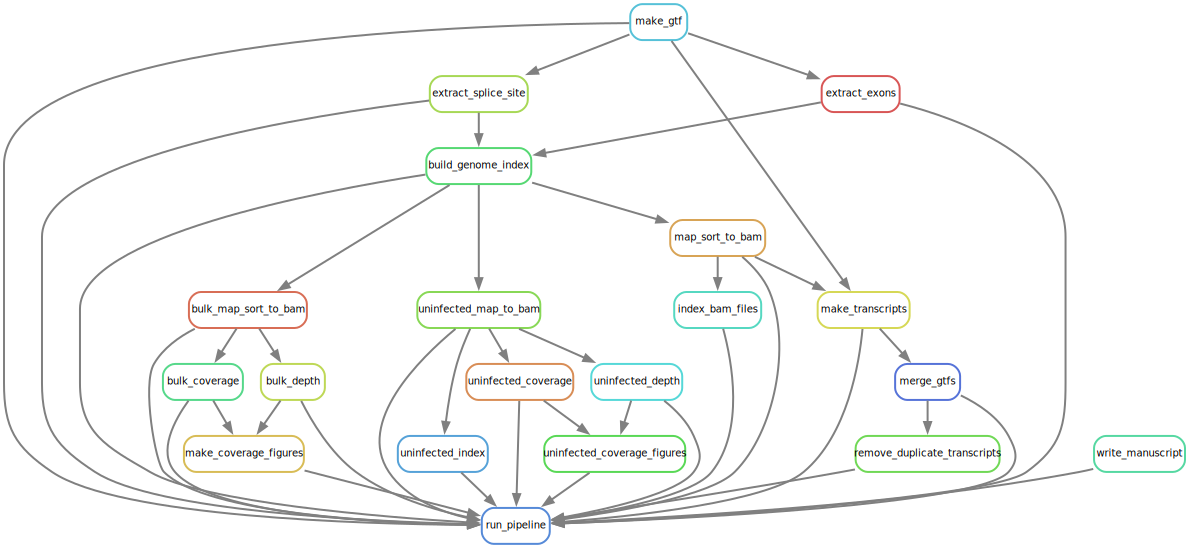
\includegraphics{project_map.png}
\caption{A flowchart of the major steps in the computational analysis
pipeline (\emph{generated with Snakemake})}
\end{figure}

\end{document}
